% This is the Reed College LaTeX thesis template. Most of the work
% for the document class was done by Sam Noble (SN), as well as this
% template. Later comments etc. by Ben Salzberg (BTS). Additional
% restructuring and APA support by Jess Youngberg (JY).
% Your comments and suggestions are more than welcome; please email
% them to cus@reed.edu
%
% See http://web.reed.edu/cis/help/latex.html for help. There are a
% great bunch of help pages there, with notes on
% getting started, bibtex, etc. Go there and read it if you're not
% already familiar with LaTeX.
%
% Any line that starts with a percent symbol is a comment.
% They won't show up in the document, and are useful for notes
% to yourself and explaining commands.
% Commenting also removes a line from the document;
% very handy for troubleshooting problems. -BTS

% As far as I know, this follows the requirements laid out in
% the 2002-2003 Senior Handbook. Ask a librarian to check the
% document before binding. -SN

%%
%% Preamble
%%
% \documentclass{<something>} must begin each LaTeX document
\documentclass[12pt,oneside]{reedthesis}
% Packages are extensions to the basic LaTeX functions. Whatever you
% want to typeset, there is probably a package out there for it.
% Chemistry (chemtex), screenplays, you name it.
% Check out CTAN to see: http://www.ctan.org/
%%
\usepackage{graphicx,latexsym}
\usepackage{amsmath}
\usepackage{amssymb,amsthm}
\usepackage{longtable,booktabs,setspace}
\usepackage{chemarr} %% Useful for one reaction arrow, useless if you're not a chem major
\usepackage[hyphens]{url}
% Added by CII
\usepackage[hidelinks]{hyperref}
\usepackage{lmodern}
\usepackage{float}
\floatplacement{figure}{H}
% End of CII addition
\usepackage{rotating}

% Next line commented out by CII
%%% \usepackage{natbib}
% Comment out the natbib line above and uncomment the following two lines to use the new
% biblatex-chicago style, for Chicago A. Also make some changes at the end where the
% bibliography is included.
%\usepackage{biblatex-chicago}
%\bibliography{thesis}


% Added by CII (Thanks, Hadley!)
% Use ref for internal links
\renewcommand{\hyperref}[2][???]{\autoref{#1}}
\def\chapterautorefname{Chapter}
\def\sectionautorefname{Section}
\def\subsectionautorefname{Subsection}
% End of CII addition

% Added by CII
\usepackage{caption}
\captionsetup{width=5in}
% End of CII addition

% \usepackage{times} % other fonts are available like times, bookman, charter, palatino

% Syntax highlighting #22
  \usepackage{color}
  \usepackage{fancyvrb}
  \newcommand{\VerbBar}{|}
  \newcommand{\VERB}{\Verb[commandchars=\\\{\}]}
  \DefineVerbatimEnvironment{Highlighting}{Verbatim}{commandchars=\\\{\}}
  % Add ',fontsize=\small' for more characters per line
  \usepackage{framed}
  \definecolor{shadecolor}{RGB}{248,248,248}
  \newenvironment{Shaded}{\begin{snugshade}}{\end{snugshade}}
  \newcommand{\KeywordTok}[1]{\textcolor[rgb]{0.13,0.29,0.53}{\textbf{#1}}}
  \newcommand{\DataTypeTok}[1]{\textcolor[rgb]{0.13,0.29,0.53}{#1}}
  \newcommand{\DecValTok}[1]{\textcolor[rgb]{0.00,0.00,0.81}{#1}}
  \newcommand{\BaseNTok}[1]{\textcolor[rgb]{0.00,0.00,0.81}{#1}}
  \newcommand{\FloatTok}[1]{\textcolor[rgb]{0.00,0.00,0.81}{#1}}
  \newcommand{\ConstantTok}[1]{\textcolor[rgb]{0.00,0.00,0.00}{#1}}
  \newcommand{\CharTok}[1]{\textcolor[rgb]{0.31,0.60,0.02}{#1}}
  \newcommand{\SpecialCharTok}[1]{\textcolor[rgb]{0.00,0.00,0.00}{#1}}
  \newcommand{\StringTok}[1]{\textcolor[rgb]{0.31,0.60,0.02}{#1}}
  \newcommand{\VerbatimStringTok}[1]{\textcolor[rgb]{0.31,0.60,0.02}{#1}}
  \newcommand{\SpecialStringTok}[1]{\textcolor[rgb]{0.31,0.60,0.02}{#1}}
  \newcommand{\ImportTok}[1]{#1}
  \newcommand{\CommentTok}[1]{\textcolor[rgb]{0.56,0.35,0.01}{\textit{#1}}}
  \newcommand{\DocumentationTok}[1]{\textcolor[rgb]{0.56,0.35,0.01}{\textbf{\textit{#1}}}}
  \newcommand{\AnnotationTok}[1]{\textcolor[rgb]{0.56,0.35,0.01}{\textbf{\textit{#1}}}}
  \newcommand{\CommentVarTok}[1]{\textcolor[rgb]{0.56,0.35,0.01}{\textbf{\textit{#1}}}}
  \newcommand{\OtherTok}[1]{\textcolor[rgb]{0.56,0.35,0.01}{#1}}
  \newcommand{\FunctionTok}[1]{\textcolor[rgb]{0.00,0.00,0.00}{#1}}
  \newcommand{\VariableTok}[1]{\textcolor[rgb]{0.00,0.00,0.00}{#1}}
  \newcommand{\ControlFlowTok}[1]{\textcolor[rgb]{0.13,0.29,0.53}{\textbf{#1}}}
  \newcommand{\OperatorTok}[1]{\textcolor[rgb]{0.81,0.36,0.00}{\textbf{#1}}}
  \newcommand{\BuiltInTok}[1]{#1}
  \newcommand{\ExtensionTok}[1]{#1}
  \newcommand{\PreprocessorTok}[1]{\textcolor[rgb]{0.56,0.35,0.01}{\textit{#1}}}
  \newcommand{\AttributeTok}[1]{\textcolor[rgb]{0.77,0.63,0.00}{#1}}
  \newcommand{\RegionMarkerTok}[1]{#1}
  \newcommand{\InformationTok}[1]{\textcolor[rgb]{0.56,0.35,0.01}{\textbf{\textit{#1}}}}
  \newcommand{\WarningTok}[1]{\textcolor[rgb]{0.56,0.35,0.01}{\textbf{\textit{#1}}}}
  \newcommand{\AlertTok}[1]{\textcolor[rgb]{0.94,0.16,0.16}{#1}}
  \newcommand{\ErrorTok}[1]{\textcolor[rgb]{0.64,0.00,0.00}{\textbf{#1}}}
  \newcommand{\NormalTok}[1]{#1}

% To pass between YAML and LaTeX the dollar signs are added by CII
\title{Spatio-Temporal Forecasts for Bike Availability in Dockless Bike Sharing
Systems}
\author{Lucas van der Meer}
% The month and year that you submit your FINAL draft TO THE LIBRARY (May or December)
\date{February 25, 2019}
\division{Institue for Geoinformatics}
\advisor{Prof.~Dr.~Edzer Pebesma}
\institution{University of Münster}
\degree{Master of Science}
%If you have two advisors for some reason, you can use the following
% Uncommented out by CII
\altadvisor{Prof.~Dr.~Jorge Mateu}
% End of CII addition

%%% Remember to use the correct department!
\department{}
% if you're writing a thesis in an interdisciplinary major,
% uncomment the line below and change the text as appropriate.
% check the Senior Handbook if unsure.
%\thedivisionof{The Established Interdisciplinary Committee for}
% if you want the approval page to say "Approved for the Committee",
% uncomment the next line
%\approvedforthe{Committee}

% Added by CII
%%% Copied from knitr
%% maxwidth is the original width if it's less than linewidth
%% otherwise use linewidth (to make sure the graphics do not exceed the margin)
\makeatletter
\def\maxwidth{ %
  \ifdim\Gin@nat@width>\linewidth
    \linewidth
  \else
    \Gin@nat@width
  \fi
}
\makeatother

\renewcommand{\contentsname}{Table of Contents}
% End of CII addition

\setlength{\parskip}{0pt}

% Added by CII
  %\setlength{\parskip}{\baselineskip}
  \usepackage[parfill]{parskip}

\providecommand{\tightlist}{%
  \setlength{\itemsep}{0pt}\setlength{\parskip}{0pt}}

\Acknowledgements{
This thesis, and in the broader sense, my whole period as a student,
would not have been possible without the help and support of others. It
still feels somewhat strange, that by writing these words, a seven-year
journey comes to an end. I want to thank my family, and in particular my
parents, for their unconditional support, also in times when I made
wrong decisions. Lorena, thank you for cheering me up whenever I needed
it, and my friends and classmates, thank you for being like a family!\\
I want to thank all my teachers for sharing their knowledge, despite
making me suffer with homework and assignments! In particular, I want to
thank my supervisor, Edzer Pebesma, for providing guidance whenever
necessary, but also constantly encouracing an independent way of working
and thinking, in which own thoughts and ideas are important.
Additionally, I want to thank my co-supervisors, Jorge Mateu and Joel
Silva, for their valuable feedback. Thanks also to the whole r-spatial
community, for providing open source tools, and encouraging involvement
and contributions, within an environment that makes everyone feel
equally valued.\\
Finally, I owe gratitude to JUMP Bikes, and Alexander Tedeschi in
particular, for providing me with very useful data.
}

\Dedication{

}

\Preface{

}

\Abstract{
The preface pretty much says it all. \par

Second paragraph of abstract starts here.
}

	\usepackage{caption}
	\usepackage{array}
	\usepackage{booktabs}
	\usepackage{makecell}
	\usepackage{longtable}
	\usepackage{multirow}
	\usepackage{wrapfig}
	\usepackage{float}
	\usepackage{colortbl}
	\usepackage{pdflscape}
	\usepackage{tabu}
	\usepackage{threeparttable}
	\usepackage{threeparttablex}
	\usepackage[normalem]{ulem}
	\usepackage{xcolor}
	\usepackage{wrapfig}
	\usepackage{graphicx}
	\usepackage{parskip}
	\usepackage[font=footnotesize,labelfont=bf, width=\textwidth]{caption}
	\usepackage[hidelinks]{hyperref}
	\usepackage[T1]{fontenc}
% End of CII addition
%%
%% End Preamble
%%
%
\begin{document}

% Everything below added by CII
  \maketitle

\frontmatter % this stuff will be roman-numbered
\pagestyle{empty} % this removes page numbers from the frontmatter
  \begin{acknowledgements}
    This thesis, and in the broader sense, my whole period as a student,
    would not have been possible without the help and support of others. It
    still feels somewhat strange, that by writing these words, a seven-year
    journey comes to an end. I want to thank my family, and in particular my
    parents, for their unconditional support, also in times when I made
    wrong decisions. Lorena, thank you for cheering me up whenever I needed
    it, and my friends and classmates, thank you for being like a family!\\
    I want to thank all my teachers for sharing their knowledge, despite
    making me suffer with homework and assignments! In particular, I want to
    thank my supervisor, Edzer Pebesma, for providing guidance whenever
    necessary, but also constantly encouracing an independent way of working
    and thinking, in which own thoughts and ideas are important.
    Additionally, I want to thank my co-supervisors, Jorge Mateu and Joel
    Silva, for their valuable feedback. Thanks also to the whole r-spatial
    community, for providing open source tools, and encouraging involvement
    and contributions, within an environment that makes everyone feel
    equally valued.\\
    Finally, I owe gratitude to JUMP Bikes, and Alexander Tedeschi in
    particular, for providing me with very useful data.
  \end{acknowledgements}

  \hypersetup{linkcolor=black}
  \setcounter{tocdepth}{4}
  \tableofcontents

  \listoftables

  \listoffigures
  \begin{abstract}
    The preface pretty much says it all. \par
    
    Second paragraph of abstract starts here.
  \end{abstract}

\mainmatter % here the regular arabic numbering starts
\pagestyle{fancyplain} % turns page numbering back on

\chapter{Introduction}\label{introduction}

\section{Context}\label{context}

Over the past decades, the world has been urbanizing at a rapid pace.
Where in 1950, 30\% of the world's population lived in urban areas, this
grew to 55\% by 2018. It is a development of which the end is not yet in
sight. By 2050, the urban population is projected to have increased to
68\% (United Nations, \protect\hyperlink{ref-un2018}{2018}). Managing
the urban growth in a sustainable manner, balancing economical, social
and environmental factors, forms a tremendous challenge. One of the
cores of this challenge relates to transportation. Nowadays, urban
transport policies still have a strong focus on the private car as
leading transportation mode. However, neither from the economical,
social nor environmental perspective, this is sustainable. Air
pollution, resource depletion, fuel costs, congestion, noise, accidents
and space requirements are among the elements that set limits to a
car-oriented urban environment (Hickman \& Banister,
\protect\hyperlink{ref-hickman2014}{2014}). Therefore, on our way
towards more sustainable cities, with a high quality of life, a drastic
shift of focus is required, which includes the integration of transport
modes that provide feasible alternatives to car usage. Although changing
travel behaviours is a complex and slow process, more and more cities
across the world are acknowledging this need, and start acting upon it.

As argued by Pucher \& Buehler
(\protect\hyperlink{ref-pucher2017}{2017}), the most sustainable and
functional mode of transport in urban areas, is probably the bicycle. It
can be used for short and medium distance trips, that form a large part
of everyday city travel. Since it causes no air pollution, is healthy,
has low usage and infrastructure costs, and requires little space,
cycling is sustainable in both the economical, social and environmental
sense. Not for nothing, it receives increasing attention in cities all
over the world. The share of trips done by bicycle, has risen sharply in
recent years, also in cities without a cycling tradition, and
investments are made to improve the bicycle infrastructure. Furthermore,
urban cycling is becoming a hot topic in academia as well, with a strong
growth in the number of publications related to this topic over the last
few years (Fishman, \protect\hyperlink{ref-fishman2016}{2016}; Pucher \&
Buehler, \protect\hyperlink{ref-pucher2017}{2017}).

Public bike sharing systems (PBSS) form an important part of the shift
towards more cycling-oriented cities. They are build on the concept of a
shared utilization of bicycle fleets, in which individuals can use
bicycles whenever they need them, eliminating the costs and
responsibilities that come with private bike ownership (Shaheen, Guzman,
\& Zhang, \protect\hyperlink{ref-shaheen2010}{2010}). Especially in
cities without a cycling tradition, PBSS can normalize the image of
cycling as a legitimate mode of everyday transport (Goodman, Green, \&
Woodcock, \protect\hyperlink{ref-goodman2014}{2014}). Furthermore, the
flexibility of PBSS make them a suitable way to improve the first and
last mile connection to other transit modes (X.-H. Yang et al.,
\protect\hyperlink{ref-yang2018}{2018}).

The number of PBSS worldwide grew from 5 in 2005 to 1571 in 2018 (C.
Schmidt, \protect\hyperlink{ref-schmidt2018}{2018}). Although this
extraordinary growth is a relatively recent development, PBSS have been
around for much longer. Already in 1965, the first one started in
Amsterdam. This system, known as \emph{Witte Fietsen} (White Bikes),
consisted of fifty permanently unlocked, white painted bikes that were
scattered throughout the city, could be freely used, and left in any
location. However, due to theft and vandalism, the experiment became a
failure, and the system was shut down within days. It took 25 years
before a new generation of PBSS entered the stage, in Denmark, 1991. In
these systems, bikes had to be picked up and dropped off at designated
docking stations, and payments were done with coin deposits. Because of
the anonymity of the users, theft remained an issue. This lead to the
third generation PBSS, which really took hold when Lyon's Velo'v system
was introduced in 2005. Third generation PBSS used more advanced
technologies, including electronic docking stations, information
tracking, and electronic, dynamic payments with smartcards (DeMaio,
\protect\hyperlink{ref-demaio2009}{2009}; Shaheen et al.,
\protect\hyperlink{ref-shaheen2010}{2010}). Over time, this evolved into
the station-based bike sharing systems as we know them now, with the
smartcard being replaced by mobile applications.

The modern, station-based systems are organized and well manageable.
However, the accessibility of docking stations forms a large barrier for
its usage: either there are no docking stations close enough to the
desired trip origin, either there are no docking stations close enough
to the desired trip destination (Fishman, Washington, Haworth, \&
Mazzei, \protect\hyperlink{ref-fishman2014}{2014}). The possibilities of
increasing the number of docking stations are generally limited, due to
high costs and space requirements. As an answer to this inconveniences,
so-called \emph{dockless bike sharing systems}, in some literature also
referred to as \emph{free floating bike sharing sytems} or
\emph{flexible bike sharing systems}, have rapidly gained popularity in
the last few years. In 2018, an estimated 16 to 18 million dockless
shared bikes were in use, compared to 3.7 million station-based shared
bikes (C. Schmidt, \protect\hyperlink{ref-schmidt2018}{2018}).

The dockless systems build on the philosophy behind the first generation
PBSS, with bikes that can be picked up and dropped off at any location
in the city. They are, however, supported by new technologies that limit
the risk of theft and vandalism. The bicycles generally have integrated
GPS tracking and an electronic lock. Usage is simple and convenient.
Users download a mobile application and create a profile, which they
link to their credit card, or charge with money from their bank account.
On the app, they find an available bike, which they can unlock with
their smartphone, usually by scanning a QR code. The ride can be ended
anywhere, and a mobile payment is made, with the price depending on the
travel time (Shen, Zhang, \& Zhao,
\protect\hyperlink{ref-shen2018}{2018}).

The revival of dockless bike sharing systems started in 2015, when two
Chinese start-up companies, Mobike and Ofo, introduced them to several
cities in China (Sun, \protect\hyperlink{ref-sun2018}{2018}). Since that
moment, the expansion evolved extremely fast. Within one year, Mobike
was present in eighteen Chinese cities with more than a million bikes in
total, and other bike sharing start-ups emerged to follow their example
(Van Mead, \protect\hyperlink{ref-guardian1}{2017}). From 2017 on, the
systems spread across the world. In most cases, they were not welcomed
with open arms by the local authorities and inhabitants, since
regulations did not exist, and the companies simply dumped bikes
throughout the cities, fighting for the highest market share, and not
putting any effort into frequently maintaining and rebalancing the
bikes. \emph{BBC} talked about the dockless bikes that are `flooding the
world' (Belton, \protect\hyperlink{ref-bbc}{2018}), \emph{The New York
Times} named it `the bike sharing explosion' (Larmer,
\protect\hyperlink{ref-nytimes}{2017}), and \emph{The Guardian} even
used the term `bike war' (Collinson,
\protect\hyperlink{ref-guardian2}{2018}).

Currently, the peak of the storm seems to have passed, and more and more
cities have defined rules to control the dockless bike sharing
expansion. These include requirements for operators to obtain a permit
before entering the market, designated `system areas' in which the bikes
can be used, limits to the fleet size and restrictions to allowed
parking spots (Deighton-Smith, \protect\hyperlink{ref-itf2018}{2018}).
Thus, cities embrace dockless bike sharing in a well balanced way, take
advantage of its convenience, and make it an important part of the
strive to a more sustainable urban environment.

\section{Objective}\label{objective}

In order to become a serious alternative for motorized transport, PBSS
need to be organized and reliable. For station-based systems, this means
that situations in which a user either can not start a trip at the
desired time and location because of an empty docking station, or can
not end a trip at the desired time and location because of a full
docking station, should be avoided. In dockless bike sharing systems,
the latter is not an issue, since bikes can be left anywhere and
anytime. The first, however, remains a challenge. A user does not have
the certainty of finding an available bike near the desired trip origin,
at the desired time of departure.

Accurate, short-term forecasts of the distribution of available bikes
both over space and time, enable system operators to anticipate on
imbalances between supply and demand, such that the occurrence of
situations as described above is limited to a minimum. Furthermore,
users can take advantage of these forecasts also in a direct way, to
plan their trips effectively, and reduce the time spend on searching for
a bike. Hence, forecasting bike availability is of great importance when
turning the shared bike into a reliable, pleasant and uncomplicated mode
of transport.

Several approaches have been developed to forecast the bike availability
in station-based bike sharing systems. However, dockless bike sharing
systems remain fairly unexplored in that sense, since their rapid
expansion only started very recently, and in contradiction to the
station-based system, large historical data sets are not widely and
openly available.

Furthermore, the spatio-temporal nature of dockless bike sharing data
brings additional challenges to the forecasting task. In station-based
systems, forecasts are only required at fixed spatial locations, and
although some works include spatio-temporal relationships between
stations, they can mostly be treated as distinct entities, with
different forecasting models for each station. In dockless bike sharing
systems, however, available bikes can be at any spatial location inside
the system area. Besides, the bike availability not only has a spatial
dependence, with more bikes being available in certain areas, and a
temporal dependence, with more bikes being available at certain times,
but those dependencies are also linked to each other. That is, temporal
patterns may differ over space, and vice versa.

The objective of this thesis is to deal with those challenges, and
develop a generally applicable methodology for bike availability
forecasting in dockless bike sharing systems.

\section{Related work}\label{related-work}

Pal, Zhang, \& Kwon (\protect\hyperlink{ref-pal2018}{2018}) define two
main categories in which publications related to PBSS can be classified.
The first category involves the studies whose primary objective is to
forecast the system's future bike availability, bike demand, or similar.
The second category involves the studies whose primary objective is to
understand and describe the system, so that either its service level can
be improved or the system can be expanded. Since this thesis aims to
forecast bike availability, publications of the first category are the
ones of interest. In essence, they all deal with time series analysis,
and a wide range of forecasting methods has already been applied,
primarily focused on station-based PBSS. These are covered in section
1.3.1, while the first attempts targeting dockless PBSS are reviewed in
section 1.3.2.

\subsection{Forecasting in station-based
systems}\label{forecasting-in-station-based-systems}

One of the first works on bike availability forecasting was published
ten years ago, by Froehlich, Neumann, \& Oliver
(\protect\hyperlink{ref-froehlich2009}{2009}). The study had an
exploratory approach, focused on gaining a better understanding of the
spatio-temporal patterns in station-based bike sharing systems and the
factors that influence forecasts of those patterns. Some forecasting
models were selected, ranging from very simple (e.g.~a Last Value
Predictor) to slightly more complex (e.g.~a Bayesian Network). The most
accurate forecasts were made at stations with a low usage, where the
variability in the data was small. The Bayesian Network started
outperforming the simpler methods at stations with a higher usage, and a
corresponding large variability in the data. Usage intensity did not
only vary over space, but also over time. The same conclusions were
drawn in this sense, with the most accurate forecasts during the night,
and the highest difference between simple and advanced methods during
peak hours. Furthermore, the length of the forecasting window influenced
forecasts, with higher forecast errors at larger forecasting windows.
Using more historical data generally increased forecast accuracies, but
recent observations were found to have a considerably higher influence
than distant ones. External variables such as weather and special events
were not considered.

Although the conclusions of Froehlich et al.
(\protect\hyperlink{ref-froehlich2009}{2009}) seem obvious now, they
formed an important basis for further research, with more advanced
forecasting methods. Kaltenbrunner, Meza, Grivolla, Codina, \& Banchs
(\protect\hyperlink{ref-kaltenbrunner2010}{2010}) fitted Auto Regressive
Integrated Moving Average (ARIMA) models to the historical bike
availability data of each docking station in Barcelona's \emph{Bicing}
system, incorporated information from neighbouring stations into these
models, and forecasted the amount of available bicycles up to one hour
ahead. Won Yoon, Pinelli, \& Calabrese
(\protect\hyperlink{ref-won2012}{2012}) used a similar approach, but
included recurring seasonal patterns in the ARIMA models. Borgnat et al.
(\protect\hyperlink{ref-borgnat2011}{2011}), instead, split the
forecasting task in two: linear regression, with weather, usage
intensity and specific conditions like holidays as explanatory
variables, was used to forecast a non-stationary amplitude for a given
day, while an autoregressive (AR) model forecasted the hourly
fluctuations in the data.

Rixey (\protect\hyperlink{ref-rixley2013}{2013}) created linear
regression models to forecast the number of monthly rentals per docking
station. Explanatory variables such as demographic and built environment
factors were extracted from a circular buffer with a radius of 400
meters around each station. D. Singhvi et al.
(\protect\hyperlink{ref-singhvi2015}{2015}) did a comparable study, but
on a macroscopic level, arguing that aggregating stations in
neighborhoods can substantially improve predictions.

In 2014, Kaggle, a well-known online community for data scientists,
hosted a machine learning competition, in which participants were asked
to combine historical usage patterns with weather data, and forecast
bike demand in the station-based PBSS of Washington D.C. (Kaggle,
\protect\hyperlink{ref-kaggle}{2014}). The competition increased the
academic interest in bike availability forecasting with machine learning
methods, and new publications on this topic followed rapidly. Giot \&
Cherrier (\protect\hyperlink{ref-giot2014}{2014}) compared Ridge
Regression, Adaboost Regression, Random Forest Regression, Gradient Tree
Boosting Regression and Support Vector Regression by predicting
Washington's city-wide bike sharing usage up to one day ahead, inputting
both recent observations, time features (e.g.~season, day of the week,
hour of the day) and weather features (e.g.~temperature, wind speed).
Ridge Regression and Adaboost Regression turned out to be the best
performing methods. Y. Li, Zheng, Zhang, \& Chen
(\protect\hyperlink{ref-li2015}{2015}) used Gradient Tree Boosting
Regression with time and weather features. However, they first grouped
the docking stations into distinct, spatially contiguous clusters, and
forecasted the bike usage per cluster. Dias, Bellalta, \& Oechsner
(\protect\hyperlink{ref-dias2015}{2015}) attempted to simplify the task,
by using a Random Forest Regressor to forecast only if a docking station
will be either completely full, completely empty, or anything in
between.

Later, spatial relations between individual docking stations were
incorporated into the machine learning approaches, which resulted in
more sophisticated forecasting methods. Z. Yang et al.
(\protect\hyperlink{ref-yang2016}{2016}) proposed a probabilistic
spatio-temporal mobility model that considered previous check-out
records at other stations and expected trip durations to estimate the
future check-ins at each station. Subsequently, check-outs at each
station were estimated with a Random Forest Regressor, that also took
weather forecasts into account. L. Lin, He, \& Peeta
(\protect\hyperlink{ref-lin2018}{2018}) modelled station-based PBSS as a
graph, with each station being a node. Then, they applied a
Convolutional Neural Network in a form generalized for graph-structured
data, to forecast hourly bike demand. Lozano, Paz, Villarrubia, De La
Iglesia, \& Bajo (\protect\hyperlink{ref-lozano2018}{2018}) created an
automated multi-agent bike demand forecasting system for the Salamanca's
\emph{SalenBici} system, with digital `agents' that collect different
types of data, such as calendar events, weather forecasts and historical
usage. These data are then combined, and used to forecast check-ins and
check-outs separately for each station, with a Random Forest Regressor.

The Random Forest and Convolutional Neural Network approaches were
compared by Ruffieux, Spycher, Mugellini, \& Khaled
(\protect\hyperlink{ref-ruffieux2017}{2017}). Furthermore, they
differentiated themselves by forecasting bike availability in six
different cities, instead of only one. The outcomes showed that the
Random Forest Regressor works better for short-term forecasts, while
Convolutional Neural Networks are more suitable for long-term forecasts.
B. Wang \& Kim (\protect\hyperlink{ref-wang2018}{2018}) compared the
Random Forest approach to two of the latest machine learning
innovations, Long Short Term Memory Neural Networks and Gated Recurrent
Units, but found no substantial improvements in the results.

All discussed academic publications related to bike availability
forecasting in station-based PBSS are listed in Table 1.1, in
chronological order. It can be seen that machine learning methods have
received a lot of attention in recent years, compared to traditional
statistical forecasting methods such as ARIMA. The two serve the same
goal, but have a different philosophy and model development process.
Traditional statistical methods assume a functional form in advance,
concern inference and estimation, and aim at providing models that offer
insights on the data. Machine learning methods approximate the
functional form via learning inside a `black box', do not require
specifications of the model and the error distribution, and aim solely
at providing an efficient forecast (Ermagun \& Levinson,
\protect\hyperlink{ref-ermagun2018}{2018}).

Studies in the field of bike availability forecasting that make valuable
comparisons between traditional time series forecasting and machine
learning methods, are scarce. Y. Li et al.
(\protect\hyperlink{ref-li2015}{2015}) and Z. Yang et al.
(\protect\hyperlink{ref-yang2016}{2016}) included ARIMA in their
baseline methods, but only in a form that does not take any seasonal
component into account, while Dias et al.
(\protect\hyperlink{ref-dias2015}{2015}) compared a seasonal ARIMA model
with their proposed Random Forest Regressor, but without using the same
amount of data for both methods. In spatio-temporal transportation
forecasting in general, there is no clear consensus on which method is
`better'. Despite the strong increase in publications that use machine
learning, Ermagun \& Levinson
(\protect\hyperlink{ref-ermagun2018}{2018}) state that ``there is not a
certain superiority when machine learning methods are compared with
advanced statistical methods such as autoregressive integrated moving
average.''
\begin{longtable}{>{\raggedright\arraybackslash}p{3cm}>{\raggedright\arraybackslash}p{1cm}>{\raggedright\arraybackslash}p{4cm}>{\raggedright\arraybackslash}p{3cm}>{\raggedright\arraybackslash}p{3cm}}
\caption{\label{tab:stationforecasts}Publications regarding forecasts in station-based bike sharing systems, known to the author}\\
\toprule
Authors & Year & Main forecasting method & Spatial unit of analysis & Case study\\
\midrule
\endfirsthead
\caption[]{\label{tab:stationforecasts}Publications regarding forecasts in station-based bike sharing systems, known to the author \textit{(continued)}}\\
\toprule
Authors & Year & Main forecasting method & Spatial unit of analysis & Case study\\
\midrule
\endhead
\
\endfoot
\bottomrule
\endlastfoot
\rowcolor{gray!6}  Froehlich, Neumann, and Oliver & 2009 & Bayesian Network & Docking station & Barcelona\\
Kaltenbrunner et al. & 2010 & Spatial ARIMA & Docking station & Barcelona\\
\rowcolor{gray!6}  Borgnat et al. & 2011 & Linear regression and AR & Docking station & Lyon\\
Won Yoon, Pinelli, and Calabrese & 2012 & Spatial, seasonal ARIMA & Docking station & Dublin\\
\rowcolor{gray!6}  Rixey & 2013 & Linear regression & Docking station & Washington DC, Minneapolis and Denver\\
\addlinespace
Giot and Cherrier & 2014 & Ridge regression, Adaboost regression, Random Forest regression, Gradient Tree Boosting regression and Support Vector regression & City & Washington DC\\
\rowcolor{gray!6}  D. Singhvi et al. & 2015 & Linear regression & Neighbourhood & New York\\
Y. Li et al. & 2015 & Gradient Tree Boosting regression & Cluster & Washington DC\\
\rowcolor{gray!6}  Dias, Bellalta, and Oechsner & 2015 & Random Forest regression & Docking station & Barcelona\\
Z. Yang et al. & 2016 & Probabilisitc mobility model and Random Forest regression & Docking station & Hangzhou\\
\addlinespace
\rowcolor{gray!6}  Ruffieux et al. & 2017 & Random Forest regression and Convolutional Neural Network & Docking station & Namur, Essen, Glasgow, Budapest, Vienna and Nice\\
Lin, He, and Peeta & 2018 & Graph Convolutional Neural Network & Docking station & New York\\
\rowcolor{gray!6}  Lozano et al. & 2018 & Random Forest regression & Docking station & Salamanca\\
B. Wang and Kim & 2018 & Long Short Term Memory Neural Networks and Gated Recurrent Units & Docking station & Suzhou\\*
\end{longtable}
\subsection{Forecasting in dockless
systems}\label{forecasting-in-dockless-systems}

Publications regarding bike availability forecasting in dockless PBSS
can be counted on the fingers of one hand. In addition to them, a small
number of similar studies have been done in the field of dockless car
sharing, which is based on the same principles as dockless bike sharing.

Those few attempts can be divided in two groups of approaches, which are
labeled here as the \emph{grid based approach} ad the \emph{distance
based approach}. In the grid based approach, the system's operational
area, i.e.~the `system area', is divided into distinct grid cells, which
may be regularly shaped, but do not have to be. For example, the cell
boundaries may also correspond with administrative boundaries.
Subsequently, each cell is treated as being a docking station. That is,
from the historical data on locations of available vehicles, the number
of vehicles in each cell is counted at several timestamps in the past,
creating a time series of counts. Hence, for a given geographical point,
the forecasted value will be the expected number of vehicles inside the
cell that contains the point.

The distance based approach uses the historical data to calculate the
distance from a given geographical location to the nearest available
vehicle, for several timestamps in the past, creating a time series of
real-valued distances. Hence, the forecasted value will be the expected
distance from the given point to the nearest available vehicle, at a
given timestamp in the future.

The grid based approach was taken by Caggiani, Ottomanelli, Camporeale,
\& Binetti (\protect\hyperlink{ref-caggiani2017}{2017}), who were among
of the first to forecast bike availability in dockless PBSS. They did
not use a regular grid, but defined the outline of the cells with a
spatio-temporal clustering procedure, that worked as follows. Historical
time series containing daily counts of available bikes were obtained for
each zone, and clustered based on temporal patterns. Geographically
connected zones that belonged to the same temporal cluster, were
aggregated. The resulting clusters formed the spatial units of analysis,
and for each of them, the number of available bikes was forecasted one
day ahead with a Nonlinear Autoregressive Neural Network. However, at
that time, they lacked data to test their methodology on. Instead, they
used data from the station-based bike sharing system in London,
pretending each docking station to be a cluster centroid.

Yi et al. (\protect\hyperlink{ref-yi2018}{2018}) did have access to a
dataset of a dockless PBSS, in the Chinese city of Chengu, and laid a
regular grid with square cells over its systems area. Besides historical
count data of available bikes in each grid cell, they included a
categorical variable representing the time of day in their system.
Forecasting was done with a recent machine learning method, named
Convolutional Long Short Term Memory Network. J. Müller \& Bogenberger
(\protect\hyperlink{ref-muller2015}{2015}), in contradiction, used
traditional statistical methods, and focused on forecasting the number
of car bookings in a dockless car sharing system, for each ZIP-code area
in Berlin. They compared a seasonal ARIMA model with a Holt Winters
exponential smoothing model, and found acceptable and similar
forecasting errors for both of them.

The only example of the application of the distance based approach,
known to the author, is the work of Formentin, Bianchessi, \& Savaresi
(\protect\hyperlink{ref-formentin2015}{2015}). Their methodology,
focused on dockless car sharing systems, can be summarized as follows.
For a set of given locations, evenly distributed over the city,
historical location data is pre-processed into a time series of
historical distance data. A strictly linear trend is subtracted from
these time series, and if present, the seasonal component as well, using
the classical time series decomposition method. AR models are fitted to
the data that are left. Then, a model structure that is acceptable for
all time series, is identified, and serves as the general forecasting
model for the complete city. That is, for individual forecast requests,
this general model structure will be used, no matter what the location
of the request is. Only when a forecast request is located inside the
city center, the corresponding historical distance data will be
decomposed before forecasting, assuming a daily seasonal pattern. In
that case, the seasonal component will afterwards be added to the
forecast produced by the general model. The general model is updated
every month.
\begin{table}[H]

\caption{\label{tab:docklessforecasts}Publications regarding forecasts in dockless vehicle sharing systems, known to the author}
\centering
\begin{tabular}{>{\raggedright\arraybackslash}p{3cm}>{\raggedright\arraybackslash}p{1cm}>{\raggedright\arraybackslash}p{4cm}>{\raggedright\arraybackslash}p{3cm}>{\raggedright\arraybackslash}p{2cm}>{\raggedright\arraybackslash}p{1cm}}
\toprule
Authors & Year & Main forecasting method & Approach & Case study & Type\\
\midrule
\rowcolor{gray!6}  Formentin, Bianchessi, and Savares & 2015 & AR & Distance based & Milan & Car\\
Müller and Bogenberger & 2015 & ARIMA and Holt Winters ETS & Grid based & Berlin & Car\\
\rowcolor{gray!6}  Caggiani et al. & 2017 & Nonlinear Autoregressive Neural Network & Grid based & London & Bike\\
Yi et al. & 2018 & Convolutional Long Short Term Memory Network & Grid based & Chengu & Bike\\
\bottomrule
\end{tabular}
\end{table}
\section{Approach}\label{approach}

The bike availability forecasting system as proposed in this thesis
extends the methodology proposed by Formentin et al.
(\protect\hyperlink{ref-formentin2015}{2015}), and uses the distance
based approach, since it has the following advantages over the grid
based approach.
\begin{itemize}
\tightlist
\item
  Forecasts will not be dependent on the chosen spatial resolution of
  the grid.
\item
  Forecasts will not be made with count data, which would have limited
  the choice of suitable forecasting models.
\item
  Forecasts can be interpreted in the same way at every location in
  space. This in contradiction to the grid based approach, where for a
  location at the edge of a grid cell, there might as well be closer
  bikes within the neighboring cell.
\item
  Forecasts give more freedom to the user, who can decide for himself if
  he considers the forecasted distance acceptable or not. In the grid
  based approach, the cell size is fixed, and does not take into account
  that some people are willing to walk further than others.
\end{itemize}
By choosing the distance based approach, the proposed forecasting system
will involve the analysis, modelling and forecasting of time series that
each contain the distances from specific geographical locations to the
nearest available bike, at several timetamps in the past. Hence, the
data of interest are \emph{spatio-temporal} in nature, and require a
methodology that adequately deals with both their spatial and temporal
dimension. In the proposed system, the spatio-temporal nature of the
data is used as an advantage, and an approach is developed in which the
structures of time series forecasting models build at specific locations
and specific timestamps, are inherited by forecast requests for nearby
locations, and future timestamps. In that way, the need for individual
models for each forecast request, is taken out.

Throughout the thesis, the proposed forecasting system will be referred
to as the \textbf{D}ockless \textbf{B}ike \textbf{A}vailability
\textbf{F}orecasting \textbf{S}ystem (DBAFS). The focus will lay on the
design of a general methodology for it, rather than on the creation of a
fully configured, practical application. A forecast can be requested for
any location within the system area of a dockless bike sharing system,
and, theoretically, any timestamp in the future. However, short-term
forecasts, up to one day ahead, form the target, and longer forecasting
horizons will not be handled.

\section{Outline}\label{outline}

The rest of the document is structured as follows. Chapter 2 provides a
theoretical background of the concepts used in this thesis, which are
all linked to the field of time series analysis. In Chapter 3, the
methodology of the proposed forecasting system is described into detail.
Chapter 4 presents the data on which the system is tested, and describes
the experimental setup. In Chapter 5, the results of the experiments are
shown, interpreted, and discussed. Finally, Chapter 6 lists the
conclusions of this thesis.

\chapter{Theoretical background}\label{theoretical-background}

This chapter presents a brief introduction to the theory of time series
analysis. It is meant to serve as a theoretical foundation of the
concepts used in this thesis. Therefore, the focus is clearly on those
specific concepts, and the chapter should to no means be considered a
thorough overview of the complete field of study.

The chapter is divided into five sections. In the first section, a
formal definition of time series is given. The second section discusses
the main characteristics of time series. Section three describes the
different components of time series data and presents methods to split a
time series into these components. The fourth section introduces
statistical models to forecast time series, in particular the
\emph{autoregressive integrated moving average} (ARIMA) class of models.
Finally, the fifth section focuses on a specific niche within time
series analysis that is used in this thesis, namely time series
clustering.

\section{Time series definition}\label{time-series-definition}

According to Woodward, Gray, \& Elliott
(\protect\hyperlink{ref-woodward2017}{2017}), a time series can be
defined as follows:

\textbf{Definition 1} A \emph{time series} is a special type of a
stochastic process. A stochastic process \{\(Y(t); t \in T\)\} is a
collection of random variables, where \(T\) is an index set for which
all of the random variables are defined on the same sample space. When
\(T\) represents time, the stochastic process is referred to as a time
series. \(\blacksquare\)

Typically, observations are made at equally spaced time intervals, such
as every hour, every day or every year. In such cases, \(T\) takes on a
discrete set of values, and we refer to them as \emph{discrete-time time
series}. On the other hand, \emph{continuous-time time series} arise
when \(T\) takes on a continuous range of values (Brockwell \& Davis,
\protect\hyperlink{ref-brockwell2002}{2002}). In this thesis, only
discrete-time time series are analyzed.

An observed realization of the stochastic process described in
Definition 1, is referred to by Woodward et al.
(\protect\hyperlink{ref-woodward2017}{2017}) as a \emph{realization of a
time series}. Other works, such as Brockwell \& Davis
(\protect\hyperlink{ref-brockwell2002}{2002}), Shumway \& Stoffer
(\protect\hyperlink{ref-shumway2011}{2011}) and Hyndman \&
Athanasopoulos (\protect\hyperlink{ref-hyndman2018fpp}{2018}), use the
term \emph{time series} for both the data and the stochastic process of
which it is a realization. In this thesis, for the sake of simplicity,
the latter approach is used, and no notational distinction is made.

\textbf{Definition 2} A \emph{time series} is a set of observed values
\{\(y_{t}\)\} of a stochastic process \{\(Y(t); t \in T\)\}, where \(T\)
represents time. \(\blacksquare\)

From the context it will be clear whether the term time series refers to
the process (Definition 1) or its realization (Definition 2). When
clarification is needed, it is given locally.

\section{Time series characteristics}\label{time-series-characteristics}

\subsection{Autocorrelation}\label{autocorrelation}

Analyzing time series raises unique problems in statistical modelling
and inference. In conventional statistics, methods rely on the
assumptions of independent and identically distributed random variables.
However, in time series analysis, observations made at nearby moments in
time are likely to be related. That is, it is likely that there exist
internal relationships within a time series. If these relationships are
linear, they are called autocorrelation, as defined in Definition 3
(Shumway \& Stoffer, \protect\hyperlink{ref-shumway2011}{2011}).

\textbf{Defintion 3} \emph{Autocorrelation} measures the linear
correlation between two points on the same time series observed at
different times. \(\blacksquare\)

Given a sample \{\(y_{1}, y_{2}, ... , y_{n}\)\} of a time series, the
degree of dependence in the data can be assessed by computing the
\emph{autocorrelation function} (ACF), for each lag \(h\), as defined in
Equation 1 (Brockwell \& Davis,
\protect\hyperlink{ref-brockwell2002}{2002}).

\[ \hat\rho(h) = \frac{\hat\gamma(h)}{\hat\gamma(0)}, \quad -n < h < n \]

Where \(\hat\gamma(h)\) is the autocovariance function of the sample at
lag \(h\), as defined in Equation 2.

\[ \hat\gamma(h) = n^{-1}\sum_{t=1}^{n-|h|}(y_{t+|h|} - \bar{y})(y_{t} - \bar{y}), \quad -n < h < n \]

Where \(n\) is the length of the sample, \(y_{t}\) is the data value at
time \(t\), \(y_{t-|h|}\) is the data value at time \(t\) minus \(|h|\)
time periods, and \(\bar{y}\) is the mean of the sample. Whenever a time
series \{\(Y_{t}\)\} is stationary, a concept that is introduced in the
next section, the ACF of the sample \{\(y_{t}\)\} can be used as an
estimate for the ACF of \{\(Y_{t}\)\}. A time series without
autocorrelation, with zero mean and finite variance, is called
\emph{white noise}.

Conventional statistical methods can not be appropriately applied to
data that exhibit autocorrelation, since the independency assumption is
violated. The primary objective of time series analysis, therefore, is
to develop mathematical models that are appropriate to use for data with
a temporal autocorrelation structure (Shumway \& Stoffer,
\protect\hyperlink{ref-shumway2011}{2011}). Furthermore, autocorrelation
is in some cases an advantage, since an internal dependence structure
implies that past observations can be used adequately to forecast future
values.

\subsection{Stationarity}\label{stationarity}

In time series analysis, a key role is played by time series whose
statistical properties do not vary with time (Brockwell \& Davis,
\protect\hyperlink{ref-brockwell2002}{2002}). Such time series are
referred to as \emph{stationary time series}. The most restrictive form
of stationarity is defined in Definition 4 (Woodward et al.,
\protect\hyperlink{ref-woodward2017}{2017}).

\textbf{Definition 4} A time series \{\(Y(t); t \in T\)\} is
\emph{strictly stationary} if for any \(t_{1}, t_{2}, ..., t_{k} \in T\)
and any \(h \in T\), the joint distribution of
\{\(Y_{t_{1}}, Y_{t_{2}}, ..., Y_{t_{k}}\)\} is identical to that of
\{\(Y_{t_{1+h}}, Y_{t_{2+h}}, ..., Y_{t_{k+h}}\)\}. \(\blacksquare\)

However, it is often too hard to mathematically establish the
requirement of strict stationarity, since the involved distributions are
not known. For most applications, a milder form of stationarity, which
only imposes conditions on the first and second moment of a time series,
is sufficient. This is officially known as \emph{weak stationarity},
but, in time series analysis, usually just called \emph{stationarity}.
It is mathematically defined as in Definition 5 (Woodward et al.,
\protect\hyperlink{ref-woodward2017}{2017}).

\textbf{Definition 5} A time series \{\(Y(t); t \in T\)\} is
\emph{stationary} if

\(\quad \text{1) } E[Y_{t}] = \mu \quad (\text{constant for all }t)\).

\(\quad \text{2) } Var[Y_{t}] = \sigma^{2} \quad (\text{constant for all }t)\).

\(\quad \text{3) } \gamma(t_{1}, t_{2}) \text{ depends only on } t_{2} - t_{1}\).
\(\blacksquare\)

In words, this means that a time series is said to be stationary when
the mean and variance are constant over time, and the autocovariance
function only depends on the difference between two time points, and not
on the time point itself. Note here that each time series that is
strictly stationary (Definition 4), is, by definition, also stationary
(Definition 5).

Stationarity is important, since in real-world problems, it is common
that only one realization of a time series is available. That means that
each random variable in the time series is represented by a single
value. This makes it impossible to get an understanding of the
underlying probability distributions of those random variables, unless
it is assumed that their statistical properties are the same (i.e.~the
time series is stationary). In that case, the statistical properties of
the whole sample can be used to estimate the statistical properties of
each individual probability distribution. An understanding of the
underlying probability distributions, in turn, is especially important
when the goal is to forecast how the time series will behave at future
time points. When the statistical properties of the time series have
been constant over time in the past, one can simply predict that they
will remain constant in the future.

In most practical applications, non-stationary time series are the rule
rather than the exception. Luckily, by applying mathematical
transformations, it often possible to render a non-stationary time
series as, approximately, stationary. This process is referred to as
\emph{stationarizing} a time series (Nau,
\protect\hyperlink{ref-nau2018}{2018}). Stationarizing is used a lot in
statistical forecasting methods, which are discussed in section 2.4.

\subsection{Spectral entropy}\label{spectral-entropy}

Often, two separate approaches to time series analysis are defined. The
first, referred to as the \emph{time domain}, deals primarily with the
internal dependence structure in time series data, where current values
can be explained in terms of a dependence on past values, as discussed
in section 2.2.1. The second, referred to as the \emph{frequency
domain}, works with a spectral representation of the time series, in
which the original data is expressed as a weighted sum of sine and
cosine waveforms, each with their own frequency. Named after the French
mathematician Jean-Baptiste Joseph Fourier, such a representation is
commonly known as a \emph{Fourier representation} or \emph{Fourier
series}, and its corresponding sine and cosine terms as \emph{Fourier
terms}. Forecasting is inherently tied to the time domain of time series
analysis, which will therefore be the focus of this thesis. However,
there is no schism dividing the two approaches. That is, some frequency
domain techniques can be useful even in the time domain, and vice versa
(Shumway \& Stoffer, \protect\hyperlink{ref-shumway2011}{2011}).

One of such techniques is the calculation of the spectral entropy of a
time series, which describes the order and regularity of a time series,
based on its Fourier representation. The spectral entropy of a time
series can be calculated with Equation 2.x.

\[ H = \int_{-\pi}^{\pi} \hat{f}(\lambda)\log \hat{f}(\lambda)d\lambda\]

Where \(\hat{f}_{y}(\lambda)\) is the estimated spectral density
function, which describes the importance of the different frequencies in
the Fourier representation of the time series. Usually, \(H\) is
normalized to the range of values between 0 and 1. For a detailed
description of the calculations, see Goerg
(\protect\hyperlink{ref-goerg2013}{2013}). Spectral entropy is useful in
forecasting, since it can serve as a quantative measure of the
forecastability of a time series. Data that are easy to forecast, will
have a small value of \(H\), while very noisy data will have a large
value of \(H\) (T. S. Talagala, Hyndman, \& Athanasopoulos,
\protect\hyperlink{ref-talagala2018}{2018}).

\section{Time series components}\label{time-series-components}

\subsection{Definitions}\label{definitions}

A time series can consist of various underlying patterns. Each of those
patterns is considered a distinct component of the time series, with its
own properties and behaviour. Splitting a time series into its
components is known as \emph{time series decomposition}. It enables a
separate analysis of all the components, which helps to better
understand the dynamics of a time series, but can also be useful in
forecasting, as is showed later in this chapter.

Hyndman \& Athanasopoulos (\protect\hyperlink{ref-hyndman2018fpp}{2018})
define three main components of a time series: a trend-cycle component,
a seasonal component and a remainder component. For simplicity, the
trend-cycle component is usually called just the trend component, which
is done in this thesis as well.

\textbf{Definition 4} The \emph{trend component} is the combination of
the trend and cyclical pattern of a time series. A trend exists when
there is a long-term, not necessarily linear, increase or decrease in
the data. A cyclical pattern occurs when the data exhibit rises and
falls that are not of a fixed frequency. \(\blacksquare\)

\textbf{Definition 5} The \emph{seasonal component} contains the
seasonal pattern of a time series. A seasonal pattern occurs when a time
series is affected by factors such as the time of the year or the day of
the week. Seasonality is always of a fixed and known frequency.
\(\blacksquare\)

\textbf{Definition 6} The \emph{remainder component} is the remaining
variation in a time series after the trend and seasonal components are
removed. \(\blacksquare\)

There exist several different methods for the decomposition of a time
series. Most of them are based on the classical decomposition method,
which is discussed in the next section. A more sophisticated approach is
known as STL, and is covered in section 2.2.2.3.

\subsection{Classical decomposition}\label{classical-decomposition}

The oldest and simplest method for the decomposition of a time series is
referred to as classical decomposition by Hyndman \& Athanasopoulos
(\protect\hyperlink{ref-hyndman2018fpp}{2018}). They present a stepwise
approach for the use of the method, which is summarized in this section.
Classical decomposition can be applied in two different forms. In the
additive form, a time series is assumed to be the sum of its components,
as shown in Equation 2.

\[ y_{t} = T_{t} + S_{t} + R_{t} \]

In the multiplicative form, a time series is assumed to be the product
of its components, as shown in Equation 3.

\[ y_{t} = T_{t} \times S_{t} \times R_{t} \]

Where, for both Equation 2 and Equation 3, \(y_{t}\) is the data,
\(T_{t}\) is the trend component, \(S_{t}\) is the seasonal component
and \(R_{t}\) is the remainder component.

Additive decomposition is the appropriate form when the amplitude of the
variation around the trend is relatively constant. On the other hand,
when the amplitude of the variation around the trend changes with the
level of the trend, multiplicative decomposition should be used.

In both the additive and multiplicative form of classical decomposition,
the first step is to estimate the trend component. This is done by
smoothing the data with a symmetric moving average filter of order
\(m\), where \(m\) is a non-negative integer. That is, the estimate of
the trend component at time \(t\) is the average of all the data values
within a window of \(m\) time periods centered at \(t\), as shown in
Equation 4. Usually, \(m\) is set to be equal to the seasonal period of
the time series, which, in turn, is the number of observations per
seasonal cycle. For example, when working with daily data that show a
weekly seasonal pattern, the seasonal period is 7.

\[ \hat{T}_{t} = \frac{1}{m}\sum_{j=-k}^{k}y_{t+j} \]

Where \(k = (m-1)/2\). The detrended time series data are then
calculated by removing the estimated trend component from the original
data. In the case of additive decomposition by subtraction,
\(y_{t} - \hat{T}_{t}\), and in the case of multiplicative decomposition
by division, \(y_{t}/\hat{T}_{t}\).

The seasonal component is estimated by averaging the detrended data
values per season, as shown in Equation 5. Using again the example of
daily data with a weekly seasonal pattern, that would mean that the
estimated seasonal component for a specific Monday is the average value
of all Monday observations in the data set, the estimated seasonal
component for a specific Tuesday is the average value of all Tuesday
observations in the data set, and so on.

\[ \hat{S}_{t} = \frac{1}{n_{t}}\sum_{i=1}^{n_{t}}(\omega_{t})_{i} \]

Where \(\omega_{t}\) is a vector containing all the detrended values
belonging to the same season as \(y_{t}\), and \(n_{t}\) is the length
of \(\omega_{t}\). Usually, the estimated seasonal component values for
each season are adjusted such that they add up to 0 in the case of
additive decomposition and 1 in the case of multiplicative
decomposition.

Finally, the remainder component is estimated by removing both the
estimated trend component and the estimated seasonal component from the
original time series. For additive decomposition, this is done by
applying Equation 6.

\[ \hat{R}_{t} = y_{t} - \hat{T}_{t} - \hat{S}_{t} \]

For multiplicative decomposition, Equation 7 is used.

\[ \hat{R}_{t} = \frac{y_{t}}{\hat{T}_{t}\hat{S}_{t}} \]

Classical decomposition is generally praised for its simplicity, but has
several disadvantages compared to some of the more modern decomposition
methods (Hyndman \& Athanasopoulos,
\protect\hyperlink{ref-hyndman2018fpp}{2018}). As a consequence of the
use of a symmetric moving average filter, there are no trend component
estimates available for the first few and last few observations of the
time series. Therefore, also the remainder component estimate lacks
these values. This is mainly problematic when forecasting, as is showed
later in this chapter. Furthermore, the seasonal component stays
constant over all the seasonal cycles, and cannot capture slight changes
over time. Especially when working with longer time series, this may be
an inappropriate representation of the truth. Finally, classical
decomposition is not robust to extreme values in the data.

\subsection{STL decomposition}\label{stl-decomposition}

A widely used method that is based on classical decomposition, but deals
with many of the limitations mentioned above, is known as STL. It stands
for \emph{A Seasonal-Trend decomposition procedure based on Loess}, and
was developed by R. B. Cleveland, Cleveland, McRae, \& Terpenning
(\protect\hyperlink{ref-cleveland1990}{1990}). In this section, their
methodology is summarized. STL estimates all three components for every
observation in a time series, and can also handle missing values in the
data. Both the trend and seasonal component are robust and not distorted
by extreme values. Furthermore, the seasonal component is not fixed, but
can vary slightly over time.

As its name already implies, STL is based on loess, also known as
locally-weighted regression. Loess was developed by Cleveland \& Devlin
(\protect\hyperlink{ref-cleveland1988}{1988}), and is a non-parametric
regression technique, often used for smoothing, that fits weighted least
squares regression curves to local subsets of a data set. Joining them
together forms the loess regression curve \(\hat{g}(x)\). More
specifically, for each value of \(x\), \(\hat{g}(x)\) is computed in the
following way. First, a positive integer \(q\) is chosen, which defines
the neighbourhood width. That is, the \(q\) observations that are
closest to \(x\) are selected as neighbours of \(x\). Each of these
observations is given a weight based on its distance to x, in a way that
the closest observations get the highest weight. Let \(W\) be the
tricube weight function as defined in Equation 8.

\[
W(u) = 
    \begin{cases}
      (1 - u^{3})^{3} &\quad 0 \leq u < 1\\
      0 &\quad u \geq 1\\
    \end{cases}
\]

Then, the neighbourhood weight for each observation \(x_{i}\) is
calculated with Equation 9.

\[ \upsilon_{i} = W\Bigg(\frac{|x_{i} - x|}{\lambda_{q}(x)}\Bigg) \]

Where \(\lambda_{q}(x)\) is the distance of the \(q\)th farthest
observation from \(x\). Then, \(\hat{g}(x)\) is calculated by fitting a
polynomial regression of degree \(d\) to x, using weighted least squares
with the neighbourhood weights \(\upsilon_{i}\). Usually, \(d\) is
either \(1\) or \(2\), corresponding respectively to a locally-linear
regression and a locally-quadratic regression. Since the loess
regression curve is smooth, there is no need to compute \(\hat{g}(x)\)
at all possible values of \(x\). In general, the computation of
\(\hat{g}(x)\) as described above is only performed at a finite set of
locations, and interpolated elsewhere.

STL uses loess for several smoothing operations, that, when performed on
a time series, lead to estimations of the trend, seasonal and remainder
components of the data. The method is build up of two loops: an inner
loop nested inside an outer loop. In the inner loop, the estimates of
the seasonal and trend component are updated once, in a stepwise manner,
which is described below.

\textbf{Step 1.} The inner loop starts with computing the detrended time
series data \(y_{t} - \hat{T}_{t}\) from the original time series data
\(y_{t}\). In the initial pass through the inner loop, there is no
estimation of \(T_{t}\) yet, and \(\hat{T}_{t}\) is set equivalent to
\(0\). That is, it is assumed there is no trend at all. This may be a
rather poor estimate, but inside the loop, it will soon be updated to
something more reasonable. In all successive passes through the loop,
the estimated trend component that resulted from the previous loop is
used.

\textbf{Step 2.} In the second step, the detrended time series is split
up into subsets, with each subset containing all the data belonging to
one specific season. That is, there will be \(n_{p}\) different subsets,
where \(n_{p}\) is the number of observations per seasonal cycle. Each
of those subsets is smoothed by loess, with \(q = n_{s}\) and \(d = 1\).
\(n_{s}\) is referred to as the seasonal smoothing parameter and its
value must be chosen by the analyst. It basically determines how much
the seasonal component is allowed to change over time. High values of
\(n_{s}\) allow little variation, while low values can lead to
overfitting. The smoothed values of all the subsets are then binded back
together into a temporary seasonal component \(C_{t}\). Each end of
\(C_{t}\) is extended \(n_{p}\) positions, such that \(C_{t}\) has
\(2 \times n_{p}\) observations more than the original time series.

\textbf{Step 3.} In the third step, any trend that may have contaminated
\(C_{t}\) is identified. This is done by applying a sequence of
smoothers, called a low-pass filter, to \(C_{t}\). It starts with a
moving average of length \(n_{p}\), followed by another moving average
of length \(n_{p}\), followed by a moving average of length 3, followed
by a loess smoothing with \(q = n_{l}\) and \(d = 1\). Just as earlier
with \(n_{s}\), the low-pass filter smoothing parameter \(n_{l}\) should
be chosen by the analyst. The output of the third step is called
\(L_{t}\). Since moving averages are used, the first \(n_{p}\)
observations and the last \(n_{p}\) observations of \(C_{t}\) will not
have a smoothed value in \(L_{t}\). However, this was already accounted
for by extending \(C_{t}\) in step 2. That is, \(L_{t}\) is again of the
same length as the original time series.

\textbf{Step 4.} In the fourth step, the seasonal component is estimated
by detrending the temporary seasonal component. That is,
\(\hat{S}_{t} = C_{t} - L_{t}\).

\textbf{Step 5.} In the fifth step, the deseasonalized time series data
\(y_{t} - \hat{S}_{t}\) are computed from the original time series data
\(y_{t}\).

\textbf{Step 6.} In the sixth and last step of the inner loop, the
estimation of the trend component, \(\hat{T}_{t}\), is calculated by
loess smoothing the deseasonalized time series with \(q = n_{t}\) and
\(d = 1\). The trend smoothing parameter \(n_{t}\) should be chosen by
the analyst.

The outer loop of STL starts with \(n_{i}\) iterations of the inner
loop. The estimations of the trend and seasonal components that follow
from the passes through the inner loop, are used to estimate the
remainder component with Equation 10.

\[ \hat{R}_{t} = y_{t} - \hat{T}_{t} - \hat{S}_{t} \]

For each observation in the time series, a robustness weight is
calculated. This weight reflects how extreme the value of the remainder
component of that observation is, in a way that a very extreme value is
given a very low, or even zero, weight. Let \(B\) be the bisquare weight
function as defined in Equation 11.

\[
B(u) = 
    \begin{cases}
      (1 - u^{2})^{2} &\quad 0 \leq u < 1\\
      0 &\quad u \geq 1\\
    \end{cases}
\]

Then, the robustness weight at time point \(t\) is calculated with
Equation 12.

\[ \rho_{t} = B\Bigg(\frac{|R_{t}|}{6median(|R_{t}|)}\Bigg) \]

After the first pass of the outer loop, the next iteration starts again
with \(n_{i}\) passes through the inner loop. However, in the loess
smoothing in step 2 and step 6, each neighbourhood weight
\(\upsilon_{t}\) is now multiplied by its corresponding robustness
weight \(\rho_{t}\), such that extreme values have less influence on the
estimates of the trend and seasonal components. Also, the estimated
trend component that resulted from the last inner loop in the previous
outer loop, is now used as first value of \(\hat{T}_{t}\), rather than
\(0\). In total, the outer loop is carried out \(n_{o}\) times.

STL is designed for additive decomposition. However, a multiplicative
version can be obtained by first log transforming the data, and finally
back-transforming the components. This is based on the logarithm product
rule, which states that \(log(a) + log(b)\) is equivalent to
\(log(a \times b)\) (Hyndman \& Athanasopoulos,
\protect\hyperlink{ref-hyndman2018fpp}{2018}).

The complete methodology of STL as described above is summarized in
Figure 1.
\begin{figure}[h]
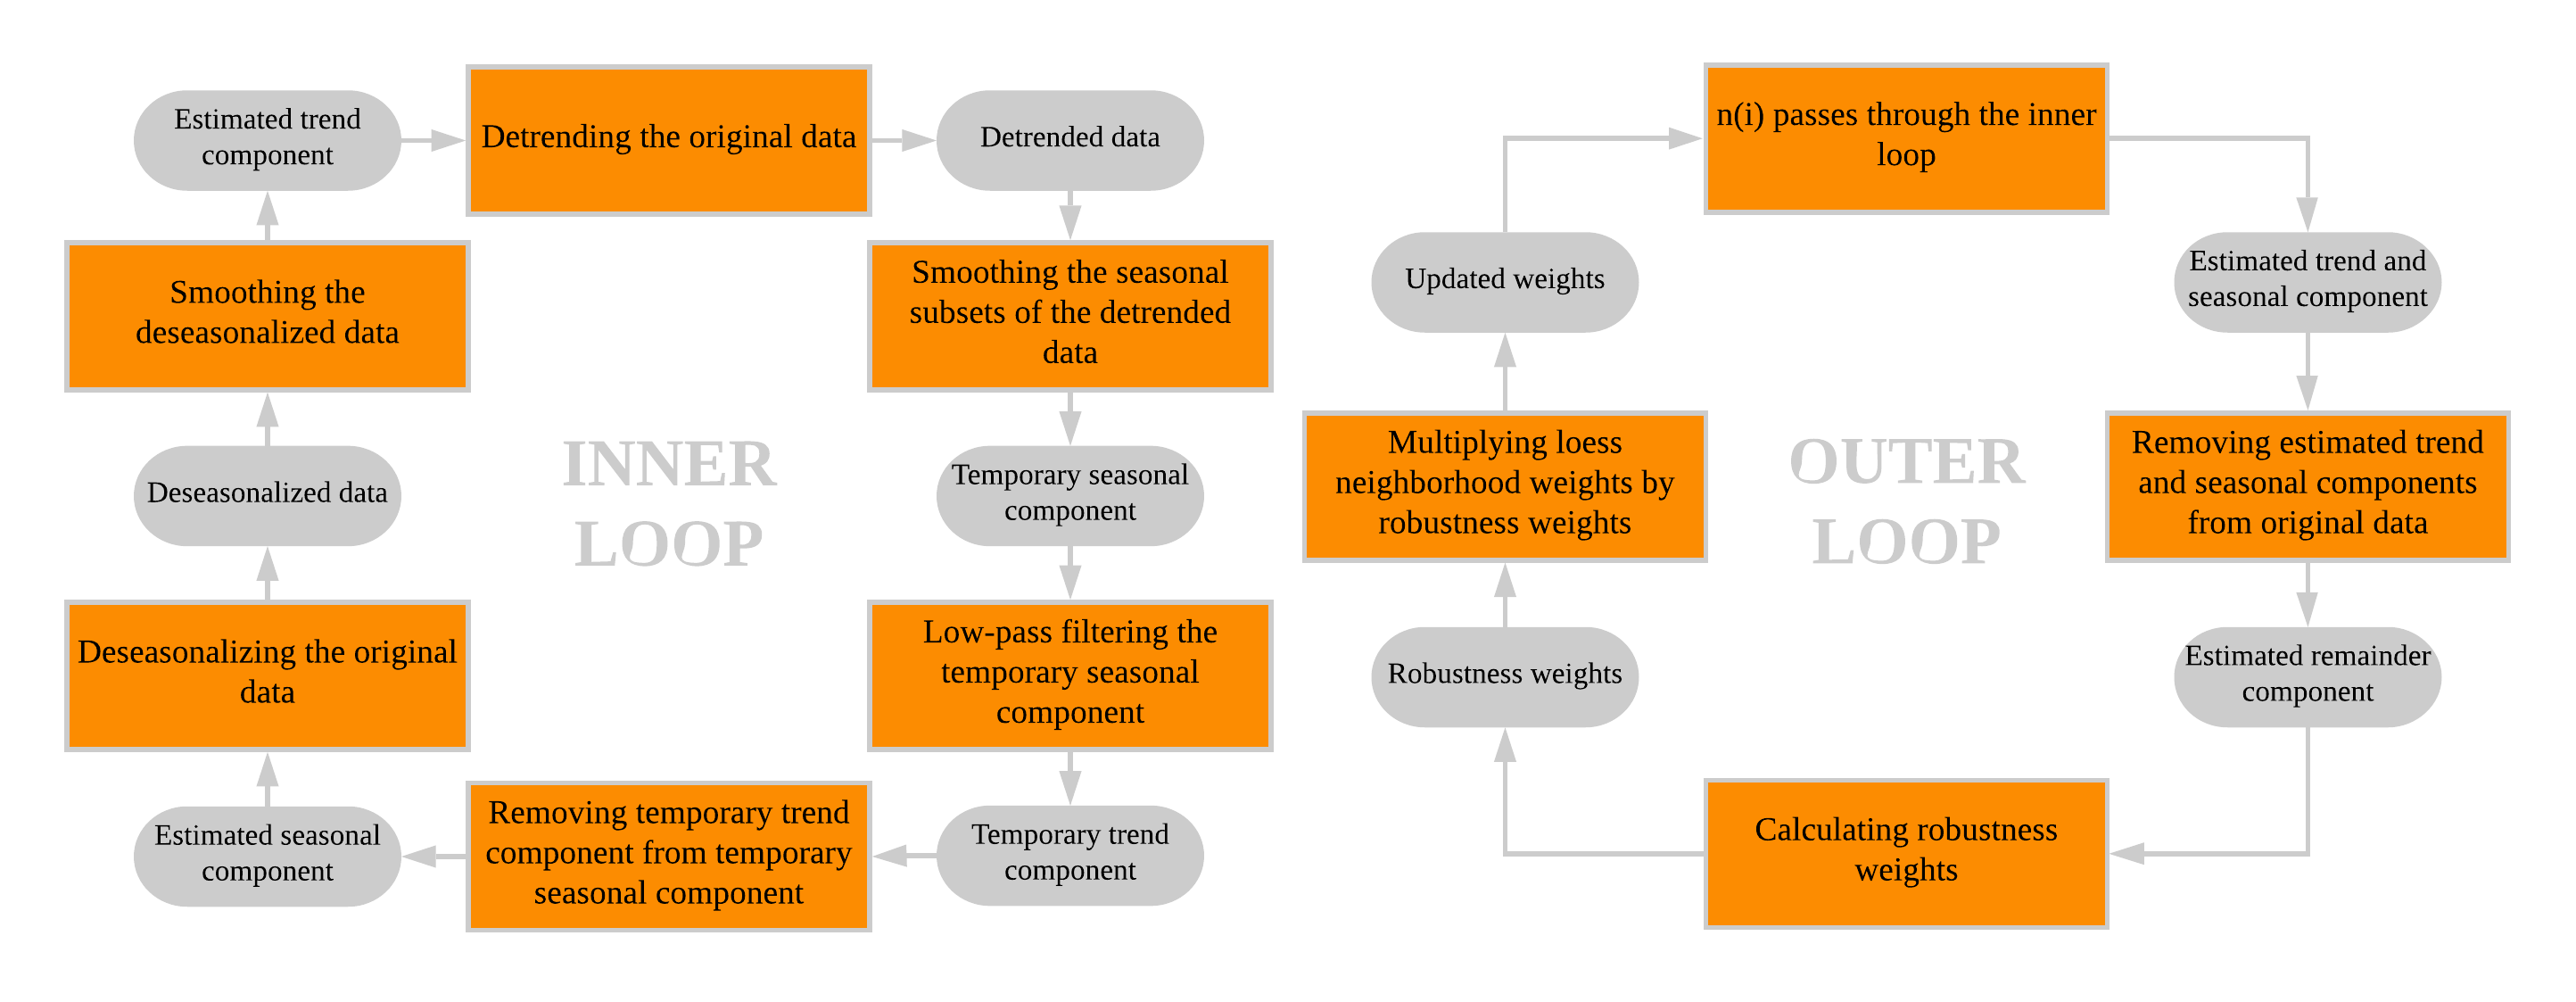
\includegraphics[width=\textwidth]{Figures/STL} \caption{Summary of the STL methodology}\label{fig:stl}
\end{figure}
\section{Time series forecasting}\label{time-series-forecasting}

\subsection{Forecasting models}\label{forecasting-models}

Often, the main aim of time series analysis is to forecast future values
of a time series. In some cases, this can be done by using external
exploratory variables. One could for example try to forecast the profit
of ice cream sales by using air temperature as an exploratory variable
in a linear regression model. However, there are several reasons not to
forecast time series in this way, as summed up by Hyndman \&
Athanasopoulos (\protect\hyperlink{ref-hyndman2018fpp}{2018}). Firstly,
the underlying system of the forecasted time series may not be
sufficiently understood, and even if it is, the relations with
exploratory variables may be too complex. Secondly, when forecasting
future values of a time series, also the future values of the
exploratory variables should be known, which means that each exploratory
variable should be forecasted separately before the response variable
can be forecasted. This may be too difficult to do accurately, and even
when it is possible, it remains a very time consuming task. Especially
when the only aim is to know what will happen, and not why it will
happen, it is not worth the effort. Finally, modelling a time series
with conventional statistical method like linear regression will likely
result in model errors that exhibit autocorrelation, which implies that
such models are not able to capture all the dynamics of the data. Thus,
produced forecast are not as efficient, and, probably, not as accurate
as can be.

Instead, in time series analysis, the internal dependence structure of a
time series is used to forecast future values as a function of the
current and past values (Shumway \& Stoffer,
\protect\hyperlink{ref-shumway2011}{2011}). Obviously, this primarily
requires a good understanding of that structure, which is obtained by
describing the process that generated the data with a time series model,
as defined in Definition 7, adapted from Brockwell \& Davis
(\protect\hyperlink{ref-brockwell2002}{2002}).

\textbf{Definition 7} A \emph{time series model} for an observed
realization \{\(y_{t}\)\} of a time series \{\(Y_{t}\)\} is a
specification of the joint distributions, or possibly only the means,
variances and covariances, of the random variables that \{\(Y_{t}\)\}
comprises. \(\blacksquare\)

One of the most famous and widely used groups of time series models is
known as the \emph{autoregressive integrated moving average} (ARIMA)
class of models, developed by Box \& Jenkins
(\protect\hyperlink{ref-box1970}{1970}). In this thesis, ARIMA is used
as well. The next section gives a summary of its theory, based on
Brockwell \& Davis (\protect\hyperlink{ref-brockwell2002}{2002}),
Chapter 5, Shumway \& Stoffer
(\protect\hyperlink{ref-shumway2011}{2011}), Chapter 3, and Hyndman \&
Athanasopoulos (\protect\hyperlink{ref-hyndman2018fpp}{2018}), Chapter 3
and 8.

\subsection{ARIMA}\label{arima}

\subsubsection{2.4.2.1 Structure}\label{structure}

An ARIMA model is a combination of an \emph{autoregressive} (AR) and
\emph{moving average} (MA) model, preceded by a differencing operation
on the original data. An autoregressive model of order \(p\), commonly
referred to as an AR(\(p\)) model, is based on the assumption that the
current value of a time series is a linear combination of \(p\) previous
values, as showed in Equation 13.

\[ y_{t} = \phi_{1}y_{t-1} + \phi_{2}y_{t-2} + ... + \phi_{p}y_{t-p} + \epsilon_{t} \]

Where \(y_{t}\) is the current value of the time series at time period
\(t\), \(\epsilon_{t}\) is the random error (i.e.~white noise) at time
\(t\), \(\phi_{1},...,\phi_{p}\) are model parameters.

A moving average model of order \(q\), commonly referred to as an
MA(\(q\)) model, is based on the assumption that the current value of a
time series is a linear combination of \(q\) previous errors, as showed
in Equation 14.

\[ y_{t} = \epsilon_{t} + \theta_{1}\epsilon_{t-1} + \theta_{2}\epsilon_{t-2} + ... + \theta_{q}\epsilon_{t-q} \]

Where \(y_{t}\) is the current value of the time series at time period
\(t\), \(\epsilon_{t}\) is the error at time period \(t\), which is
assumed to be white noise, and \(\theta_{1},...,\theta_{q}\) are model
parameters.

AR(\(p\)) and MA(\(q\)) models can be combined into an autoregressive
moving average model of order (\(p\), \(q\)), commonly referred to as
ARMA(\(p\), \(q\)). That is, in such a model, the current value of a
time series is a linear combination of both \(p\) previous values and
\(q\) previous errors, as showed in Equation 15.

\[ 
y_{t} = \phi_{1}y_{t-1} + ... + \phi_{p}y_{t-p} + \theta_{1}\epsilon_{t-1} + ... + \theta_{q}\epsilon_{t-q} + \epsilon_{t} 
\]

ARMA(\(p\), \(q\)) models require the forecasted time series to be
stationary. When working with non-stationary time series, it is often
possible to stationarize the series by differencing it one or more
times. The first order difference of a time series is the series of
changes from one time period to the next, as shown in Equation 16.

\[ \nabla y_{t} = y_{t} - y_{t-1} \]

Where \(\nabla y_{t}\) is the first order difference of \(y_{t}\). When
the first order difference is still non-stationary, the second order
difference \(\nabla^{2}y_{t}\) can be computed by taking again the first
order difference of \(\nabla y_{t}\), and so on. The original
non-stationary time series that needed to be differenced in order to get
stationary, is called an \emph{integrated} version of the stationary
series. That is why a model that first stationarizes the data by
applying a \(d\)-th order difference, before fitting an ARMA(\(p\),
\(q\)) model, is called an autoregressive integrated moving average
model of order (\(p\), \(d\), \(q\)), commonly referred to as
ARIMA(\(p\), \(d\), \(q\)). That is, in such a model, the current value
of the \(d-\)th order difference of a time series is a linear
combination of both \(p\) previous values and \(q\) previous errors, as
showed in Equation 17.

\[ 
\nabla^{d}y_{t} = \phi_{1}\nabla^{d}y_{t-1} + ... + \phi_{p}\nabla^{d}y_{t-p} + \theta_{1}\epsilon_{t-1} + ... + \theta_{q}\epsilon_{t-q} + \epsilon_{t} 
\]

Where \(\nabla^{d}y_{t}\) is the \(d\)-th order difference of \(y_{t}\).
Note here that ARIMA(\(p\), \(d\), \(q\)) is a general form of all the
other models discussed earlier in this section. For example, an AR(1)
model can also be written as ARIMA(1,0,0), an ARMA(2,1) as ARIMA(1,0,2),
and so on.

The process of finding an appropriate ARIMA(\(p\), \(d\), \(q\)) model
that represents a time series is known as the Box-Jenkins modelling
procedure and consists of three stages, named model selection, parameter
estimation and model checking. All these stages are described separately
in the next three subsections.

\subsubsection{2.4.2.2 Model selection}\label{model-selection}

In the model selection stage, \(p\), \(d\) and \(q\) are chosen. In this
process, \(d\) is selected first, such that the choice of \(p\) and
\(q\) will be based on a stationary time series. An appropriate value
for \(d\) can be found by inspecting the plotted data \(y_{t}\), with
time on the x-axis, and define visually if the data are stationary. If
not, then difference the data once, and inspect the plot of
\(\nabla y_{t}\). If \(\nabla y_{t}\) does not seem stationary either,
take the second-order difference \(\nabla^{2} y_{t}\), and so on. In
general, however, it is not recommended to difference more than two
times. As an addition to the time plots, plotting the sample
autocorrelation function of the data can help to identify stationarity.
Non-stationary data show a slow decay in autocorrelation as the time lag
increases, while for stationary data, the autocorrelation will drop to
zero relatively fast.

Once \(d\) has been set, either \(p\) or \(q\) can be selected by
inspecting the autocorrelation function plot and the partial
autocorrelation function plot of the differenced data, which
respectively plot the sample autocorrelation function (ACF), defined in
Equation 2.x, and the sample partial autocorrelation function (PACF),
for several lags \(h\). The PACF is the relationship between an
observation at time \(t\) and and observation at time \(t-k\), removing
the effects of all time lags in between, i.e. \(1, 2, ..., k-1\). Then,
appropriate values for either \(p\) or \(q\) are found with the
following rules of thumb:
\begin{itemize}
\tightlist
\item
  The PACF plot of an ARIMA(\(p\),\(d\),\(0\)) process cuts of after lag
  \(p\), and the ACF plot tails off.
\item
  The ACF plot of an ARIMA(\(0\),\(d\),\(q\)) process cuts of after lag
  \(q\), and the PACF plot tails off.
\end{itemize}
When dealing with ARIMA(\(p\), \(d\), \(q\)) processes where both
\(p > 0\) and \(q > 0\), the ACF plot and PACF plot will both tail off,
and finding appropriate values for \(p\) and \(q\) turns into a
trial-and-error approach, where models with different combinations of
\(p\) and \(q\) are compared.

The methodology as described above is used often, but involves a lot of
manual interventions. This makes it a rather subjective way of working,
that is labour intensive, especially when a large number of time series
needs to be modelled, and requires expert knowledge. Therefore, several
automated approaches to select \(p\), \(d\) and \(q\) have been
proposed. One of them is the Hyndman-Khandakar algorithm, which
methodology is summarized below, in a simplified way. For the full
details, see Hyndman \& Khandakar
(\protect\hyperlink{ref-forecast}{2008}).

\textbf{Step 1.} To define \(d\), the Hyndman-Khandakar algorithm uses
the Kwiatkowski-Phillips-Schmidt-Shin (KPSS) test, which is a
statistical test used to determine stationarity of a time series. Only
if there is enough statistical evidence, the null hypothesis that the
time series is stationary will be rejected, and the time series is
instead considered to be non-stationary. The detailed mathematics
underlying the test can be found in Kwiatkowski, Phillips, Schmidt, \&
Shin (\protect\hyperlink{ref-kwiat1992}{1992}).

Using the KPSS test, first, the original data \(y_{t}\) are tested for
stationarity. When \(y_{t}\) are considered stationary, \(d = 0\), and
when considered non-stationary, the first-order differenced data
\(\nabla y_{t}\) are tested for stationarity. Again, when
\(\nabla y_{t}\) are considered stationary, \(d = 1\), and when
considered non-stationary, the second-order differenced data
\(\nabla^{2} y_{t}\) are tested for stationarity. This process is
repeated until a stationary series is obtained.

\textbf{Step 2.} In the second step, four different models are fitted to
the \(d\)-times differenced data.
\begin{itemize}
\tightlist
\item
  An ARIMA(\(0\), \(d\), \(0\)) model.
\item
  An ARIMA(\(1\), \(d\), \(0\)) model.
\item
  An ARIMA(\(0\), \(d\), \(1\)) model.
\item
  An ARIMA(\(2\), \(d\), \(2\)) model.
\end{itemize}
Then, the model with the lowest AIC is selected. AIC, which stands for
Aikake's Information Criterion, is a measure for the goodness-of-fit of
a model, and can be calculated with Equation 2.x.

\[ AIC = -2 \log(L) + 2k\]

Where \(L\) is the Gaussian likelihood of the data, and \(k\) is the
number of free parameters in the model. In this case,
\(k = p + q + l + 1\), where \(l = 1\) when a non-zero constant is
included, and \(l = 0\) otherwise. The `\(+1\)' term is included, since
the variance of the residuals is also a parameter. To find the best
fitting model, AIC should be minimized. The idea behind AIC is the
following. The likelihood monotonically increases when more parameters
are added to the model, and therefore, only maximizing the likelihood
would favor a model that overfits the data. AIC prevents such
overfitting, by penalizing the likelihood with a term that is
proportional to the number of parameters used in the model.

\textbf{Step 3.} In the third step, several variations of the model that
was selected in step 2, are fitted to the \(d\)-times differenced data.
These variations include:
\begin{itemize}
\tightlist
\item
  Models where either \(p\) or \(q\) vary \(\pm 1\) from the selected
  model, given that \(p, q \ngtr 5\).
\item
  Models where both \(p\) and \(q\) vary \(\pm 1\) from the selected
  model, given that \(p, q \ngtr 5\).
\end{itemize}
From the selected model and all its variations, the model with the
lowest AIC is chosen to be the new selected model, and step 3 is
repeated. The algorithm stops when there are no variations of the
selected model that have a lower AIC. In that case, the selected model
is the optimal model, and forms the output of the Hyndman-Khandakar
algorithm. The complete methodology of the algorithm as described above
is summarized in Figure 2.x.
\begin{figure}[h]
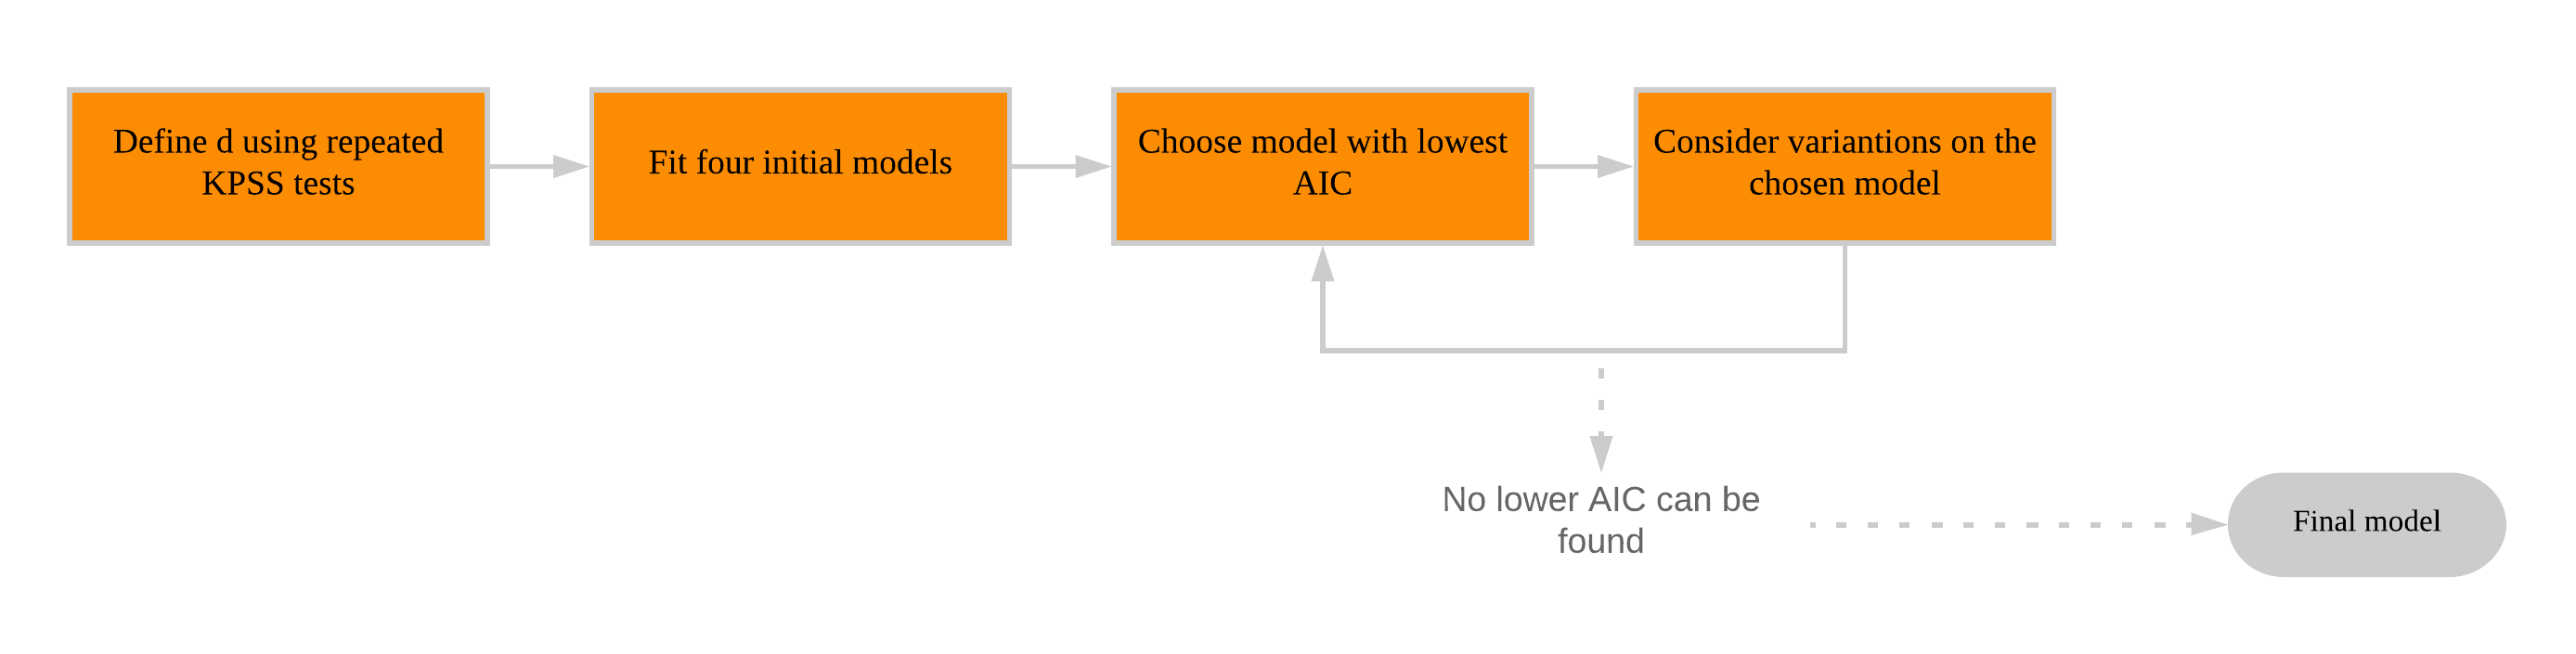
\includegraphics[width=\textwidth]{Figures/hyndman} \caption{Summary of the Hyndman-Khandakar algorithm}\label{fig:hyndman}
\end{figure}
\subsubsection{2.4.2.3 Parameter estimation}\label{parameter-estimation}

When \(p\), \(d\) and \(q\) are defined, the model parameters
\(\phi_{1},...,\phi_{p}\) and \(\theta_{1},...,\theta_{q}\) need to be
estimated. Usually, this is done with \emph{maximum likelihood
estimation} (MLE). The likelihood is the probability of obtaining the
observed data, given the model and specific parameter values. The
parameter values that maximize the likelihood are called the maximum
likelihood estimators of the true parameters, and will be used as the
parameter estimates in the fitted ARIMA(\(p\), \(d\), \(q\)) model,
which then is referred to as the maximum likelihood ARIMA(\(p\), \(d\),
\(q\)) model. The detailed mathematical description of MLE for ARIMA
models can be found in Brockwell \& Davis
(\protect\hyperlink{ref-brockwell2002}{2002}), section 5.2.

Note here that the Hyndman-Khandakar algorithm already produces a fitted
model as output, and the parameter estimation as described in this
section is done inside the algorithm, each time a model is fitted to the
\(d\)-times differenced data.

\subsubsection{2.4.2.4 Model checking}\label{model-checking}

Model checking involves identifying if the fitted model is adequate.
This is done by inspecting its residuals, which are defined as the
difference between the actual observations and the corresponding fitted
values, as shown in Equation 2.x.

\[ \epsilon_{t} = y_{t} - \hat{y}_{t} \]

If the maximum likelihood ARIMA(\(p\), \(d\), \(q\)) model is the true
process that generated the data, the residuals should be completely
white noise. Recall, however, that the model is an estimation of the
true process. Therefore, a good model that fits the data well, should
have residuals with properties that \emph{approximately} reflect those
of white noise, i.e.~a zero mean and no autocorrelation. If
autocorrelation is present in the residuals, this means that there is
still information left in the data, which could be used to create more
accurate forecasts. A non-zero mean will lead to biased forecasts.

Autocorrelation in the residuals can be detected by a visual
interpretation of the residual ACF plot, which will always show some
autocorrelation, due to random variation. Therefore, given that \(n\) is
the length of the modelled time series, and assuming a normal
distribution, the residuals are considered to be uncorrelated when for
at least 95\% of the time lags, the residual ACF lies within the
interval \([-1.96/\sqrt{n}, 1.96/\sqrt{n}]\).

Usually, several computations within the model fitting and forecasting
process build on the assumption that the data come from a normally
distributed population. For example, in MLE and the calculation of AIC,
Gaussian likelihood is commonly used. Furthermore, prediction intervals
of forecasts are in general derived from the normal distribution.
Normally distributed residuals indicate that these assumptions were
valid, and are therefore a valuable property of a model. However, as
stated by Brockwell \& Davis
(\protect\hyperlink{ref-brockwell2002}{2002}), using Gaussian likelihood
is sensible even when the data are not normally distributed.

\subsubsection{2.4.2.5 Forecasting}\label{forecasting}

A fitted ARIMA(\(p\), \(d\), \(q\)) model can then be used to forecast
the future values of a time series. To do so, Equation 2.x is rewritten,
such that the current value of the time series, \(y_{t}\), is replaced
by a future value of the time series, \(y_{t+h}\), as showed in Equation
2.x.

\[ 
\nabla^{d}y_{t+h} = \hat\phi_{1}\nabla^{d}y_{t+h-1} + ... + \hat\phi_{p}\nabla^{d}y_{t+h-p} +\hat\theta_{1}\epsilon_{t+h-1} + ... + \hat\theta_{q}\epsilon_{t+h-q} + \epsilon_{t+1} 
\]

Where \(h\) is the forecast horizon, i.e.~the number of time lags ahead
at which the forecast is made, \(p\), \(d\) and \(q\) are known and
constant, and \(\hat\phi_{1},...,\hat\phi_{p}\) and
\(\hat\theta_{1},...,\hat\theta_{q}\) are the estimated parameter
values, which are also constant.

When \(h > 1\), more than one forecast has to be made. For example, the
forecast of \(\nabla^{d}y_{t+2}\), the value of the time series two time
lags ahead, is based on \(\nabla^{d}y_{t+2-1}\), the value of the time
series one time lag ahead. Therefore, \(\nabla^{d}y_{t+2-1}\) needs to
be forecasted first, before \(\nabla^{d}y_{t+2}\) can be forecasted. In
general, this means that the uncertainty of the forecasts increases as
\(h\) increases. This uncertainty is expressed by means of a prediction
interval. Most often, the 95\% prediction interval is used. Assuming
normally distributed residuals, the lower and upper bound of the 95\%
prediction interval for the \(h\)-step forecast can be calculated with
Equation 2.x and 2.x, respectively.

\[ \ell = \hat{y}_{t+h} - 1.96\hat\sigma_{h}\]
\[ \upsilon = \hat{y}_{t+h} + 1.96\hat\sigma_{h}\]

Where \(\ell\) is the lower bound of the 95\% prediction interval,
\(\upsilon\) is the upper bound of the 95\% prediction interval,
\(\hat{y}_{t+h}\) is the forecasted value \(h\) time lags ahead.
\(\hat\sigma_{h}\) is the estimated standard deviation of the forecast
distribution \(h\) time lags ahead, which is explained below. The 95\%
prediction interval can be interpreted as follows: there is a 95\%
probability that \(\ell \leq {y}_{t+h} \leq \upsilon\).

Recall that in Definition 1, a time series was defined as a collection
of random variables. In fact, to state it statistically correct, it is
the distribution of the random variable \(h\) time lags ahead that is
forecasted, rather than an individual value. This distribution is
referred to as the forecast distribution, and the single forecasted
value, also known as the \emph{point forecast}, is then taken to be the
mean of the forecast distribution. In Equation 2.x and 2.x,
\(\hat\sigma_{h}\) is the estimated standard deviation of the forecasted
distribution, assuming it is a normal distribution with mean
\({y}_{t+h}\) and variance \(\sigma_{h}^{2}\). When \(h = 1\), the
residual standard deviation \(\sigma_{\epsilon}\) is a good estimate for
\(\sigma_{h}\). However, for \(h > 1\), computations get more complex.
For a detailed description, see Shumway \& Stoffer
(\protect\hyperlink{ref-shumway2011}{2011}), section 3.5.

\subsubsection{2.4.2.6 Accuracy evaluation}\label{accuracy-evaluation}

A good model fit, does not necessarily lead to accurate forecasts.
Therefore, when evaluating its performance, the forecasting model should
be used to forecast multiple values of new data that were not included
in the model building process. The error of each individual forecast can
be calculated with Equation 2.x.

\[ e_{t+h} = y_{t+h} - \hat{y}_{t+h} \]

Where \(y_{t+h}\) is the observed data value \(h\) time lags into the
future, and \(\hat{y}_{t+h}\) is the forecasted data value \(h\) time
lags into the future. Obviously, future in this sense is relative to the
model building period.

When making \(k\) different forecasts, the corresponding forecast errors
\(e_{1}, e_{2}, ..., e_{k}\), can be summarized with an error metric.
Several of those metrics exist. Some of them are only applicable to
errors that all have the same units, while others may also be used when
errors with different units are compared. Since all forecasts in this
thesis are distances, the unit-dependent errors are adequate. Most
commonly used are the Mean Absolute Error (MAE), which can be calculated
with Equation 2.x, and the Root Mean Squared Error (RMSE), which can be
calculated with Equation 2.x.

\[ MAE = \frac{\sum_{i = 1}^k |e_{i}|}{k} \]
\[ RMSE = \sqrt{\frac{\sum_{i = 1}^k e_{i}^{2}}{k}} \] Both the MAE and
RMSE return values that are in the same scale as the original data. The
MAE gives the same weight to all errors. The RMSE, however, gives large
errors more weight than small errors, and therefore penalizes a large
error variance. According to Chai \& Draxler
(\protect\hyperlink{ref-chai2014}{2014}), the RMSE usually is better at
revealing differences in model performance.

In some of the works discussed in section 1.3, such as Y. Li et al.
(\protect\hyperlink{ref-li2015}{2015}), Z. Yang et al.
(\protect\hyperlink{ref-yang2016}{2016}) and Lozano et al.
(\protect\hyperlink{ref-lozano2018}{2018}), the Root Mean Squared
Logarithmic Error (RMSLE) is reported instead of the RMSE. Here, the
natural logarithms of the observed and forecasted data values are used
in the forecast error computation. The main reason for doing so, is that
larger errors, usually occuring during peak hours or in areas/stations
with a high usage intensity, do not dominate smaller errors.

\subsubsection{2.4.2.7 Transformations}\label{transformations}

Often, forecasts can be improved by using mathematical transformations,
such that the original data is adjusted for some known patterns causing
non-stationary and/or non-linear behaviour. That is, the data are
transformed in advance, and the modelling and forecasting procedures are
applied to the transformed data. After forecasting the transformed data,
forecasted values on the original scale are obtained based upon the
inverse transformation, a process that is commonly called \emph{back
transforming}. A particularly useful transformation is the \emph{log
transformation}, which suppresses larger fluctuations that occur when
the level of the time series increases. Furthermore, they guarantee
strictly positive forecasted values. The log transformed data
\(\omega_{t}\), is derived by taking the natural logarithm of the
original data \(y_{t}\), as showed in Equation 2.x.

\[ \omega_{t} = \log y_{t} \]

However, care has to be taken when back transforming a log transformed
forecast to the original scale. Intuitively, one would obtain the back
transformed forecast \(\hat{y}_{t+h}\) by setting it equal to
\(e^{\hat{\omega}_{t+h}}\), where \(e\) is Euler's number. However,
assuming that the forecast distribution of \(\omega_{t+h}\),
\(\Omega_{t+h}\), is normal, with mean \(\mu_{\Omega_{t+h}}\) and
variance \(\sigma_{\Omega_{t+h}}^{2}\), then the forecast distribution
of \(y_{t+h}\), \(Y_{t+h}\), follows a log-normal distribution, with
mean \(\mu_{Y_{t+h}}\) as defined in Equation 2.x.

\[ \mu_{Y_{t+h}} = e^{(\mu_{\Omega_{t+h}} + 0.5 \sigma_{\Omega_{t+h}}^{2})} \]

For the proof of this theorem, see Dambolena, Eriksen, \& Kopcso
(\protect\hyperlink{ref-dambolena2009}{2009}). Hyndman \& Athanasopoulos
(\protect\hyperlink{ref-hyndman2018fpp}{2018}) refer to
\(\mu_{Y_{t+h}}\) as the \emph{bias-adjusted point forecast}.

\subsection{Naïve forecasts}\label{naive-forecasts}

It is common practice to compare the errors of forecasts obtained with a
fitted model to those of forecasts obtained with a very simple
forecasting method. Such a simple method, is in that case refered to as
a \emph{baseline method}. If the more sophisticated model does not lead
to considerably better forecast accuracies than the baseline, it can be
dismissed (Hyndman \& Athanasopoulos,
\protect\hyperlink{ref-hyndman2018fpp}{2018}).

One of the simplest forecast methods around, often used as a baseline,
is known as the naïve method. When forecasting with the naïve method,
all forecasted values will be equal to the last observation, no matter
how far the forecasting window \(h\) reaches, as shown in Equation 2.x.

\[ \hat{y}_{t+h} = y_{t} \]

Where \(\hat{y}_{t+h}\) is the forecasted data value \(h\) time lags
into the future, and \(y_{t}\) is the last observed data value.

\subsection{Seasonal forecasts}\label{seasonal-forecasts}

ARIMA models as described in section 2.4.2 are designed for data without
a seasonal component. With some modifications, they can be applied to
seasonal data as well. That works as follows. Instead of an ARIMA(\(p\),
\(d\), \(q\)) model, an ARIMA(\(p\), \(d\), \(q\))(\(P\), \(D\), \(Q\))
model is fitted to the data. The (\(P\), \(D\), \(Q\)) part of the model
works in a similar fashion as the (\(p\), \(d\), \(q\)) part, but
relates to the seasonal component of the data. Hence, \(P\) is the
number of seasonal autoregressive terms in the model, \(D\) is the order
of seasonal differencing, and \(Q\) is the number of seasonal moving
average terms. Where \(p = 1\) means that the past observation
\(y_{t-1}\) is used to model the current value \(y_{t}\), setting
\(P = 1\) means that the past observation \(y_{t-m}\) is used to model
the current value \(y_{t}\), with \(m\) being the number of observations
per seasonal cycle. The same holds for \(Q\): setting \(Q = 1\), means
that the past error \(\epsilon_{t-m}\) is used to model the current
value \(y_{t}\). Regarding the seasonal differencing parameter \(D\),
the first order seasonal difference of a time series is the series of
changes from one seasonal period to the next (Shumway \& Stoffer,
\protect\hyperlink{ref-shumway2011}{2011}).

However, ARIMA(\(p\), \(d\), \(q\))(\(P\), \(D\), \(Q\)), as well as
several other commonly used seasonal models such as Holt Winters
exponential smoothing, have two main limitations which make them
unsuitable for some kind of data. Firstly, they were primarily designed
to work with shorter seasonal periods, such as monthly data with
patterns that repeat every year (i.e. \(m = 12\)). In the case of longer
seasonal periods, which may occur for example in daily and sub-daily
data, modelling becomes inefficient. In the R statistical software, for
example, the \texttt{forecast} package (Hyndman \& Khandakar,
\protect\hyperlink{ref-forecast}{2008}) only allows seasonal periods up
to \(m = 350\) (Hyndman, \protect\hyperlink{ref-hyndmanblog}{2010}).

Secondly, these models can not handle more than one seasonal pattern at
a time. Again, this can be problematic especially for daily data, in
which both a weekly and yearly pattern may exist, and sub-daily data, in
which even a daily, weekly and yearly pattern may exist. One of the
alternative approaches proposed by Hyndman \& Athanasopoulos
(\protect\hyperlink{ref-hyndman2018fpp}{2018}) works as follows. First,
the data is decomposed into a trend, seasonal and remainder component.
Then, the trend and remainder component are together modelled by a
non-seasonal model, such as ARIMA(\(p\), \(d\), \(q\)), and forecasted
accordingly. The seasonal component, in turn, can be forecasted with a
seasonal naïve method, meaning that the forecasted value will be equal
to the last observed value from the same season of the year. That is,
the seasonal forecast for timestamp \(y_{t+h}\) will be equal to the
last observed value in the sequence
\{\(y_{t+h-m \times 1}, y_{t+h-m \times 2}, ...\)\}. Then, the
non-seasonal and seasonal forecasts are added back together, to obtain a
single forecasted value.

\section{Time series clustering}\label{time-series-clustering}

\subsection{Dissimilarity measures}\label{dissimilarity-measures}

Time series clustering is a specific domain within the field of time
series analysis. Given a set of individual time series, its objective is
to group similar time series into the same cluster (Keogh \& Lin,
\protect\hyperlink{ref-keogh2005}{2005}). Logically, this involves the
calculation of a measure that represents the similarity, or
dissimilarity, between two time series. A wide range of such measures
exist, some of them based directly on the observations in the time
series, others on specific features of the time series, and others on
parameters or residual characteristics of models fitted to the time
series.

Whenever the time series are of the same length, and observed at the
same timestamps, a simple dissimilarity measure can be calculated by
summing the ordered point-to-point distances between them. The most used
distance function, in this sense, is the Euclidean distance, as defined
in Equation 2.x (Cassisi, Montalto, Aliotta, Cannata, \& Pulvirenti,
\protect\hyperlink{ref-cassisi2012}{2012}).

\[ d(Y,X) = \sqrt{\sum_{t=1}^{n}(y_{t}-x_{t})^{2}} \]

Where \(d(X,Y)\) is the dissimilarity value between time series \(Y\)
and \(X\), \(y_{t}\) and \(x_{t}\) are the observations in respectively
\(Y\) and \(X\) at time \(t\), and \(n\) is the length of \(Y\) and
\(X\). A higher value of \(d(X,Y)\) implies less similar time series. By
definition, \(d(X,Y) \geq 0\).

Using Euclidean distance as a dissimilarity measure is simple, but has
drawbacks for certain applications. For example, it can not handle time
series of different length, it is sensitive to outliers, and it can not
capture out-of-phase similarities, which occur when two time series show
similar patterns, but shifted over time. To deal with one or more of
these drawbacks, several other dissimilarity measures for time series
were developed, of which the \emph{dynamic time warping distance} is
best known. Dynamic time warping is based on classical algorithms for
comparing discrete sequences with continuous sequences, and basically
replaces the one-to-one comparison of Euclidean distances with a
many-to-one comparison. However, despite its simplicity, the Euclidean
distance approach still turns out to be very competitive with the more
complex methods (Cassisi et al.,
\protect\hyperlink{ref-cassisi2012}{2012}).

Once the dissimilarity values for all possible combinations between the
analyzed time series are calculated, they are stored in an
\(n \times n\) matrix, where \(n\) is the number of analyzed time
series, and the diagonal entries equal zero. Such a matrix is commonly
referred to as a dissimilarity matrix, and can be used to cluster the
time series with conventional clustering algorithms. In time series
analysis, k-means clustering and hierarchical clustering are the most
popular options for this task (X. C. Wang, Smith, \& Hyndman,
\protect\hyperlink{ref-wang2006}{2006}). The latter is used in this
thesis, and its theory is summarized briefly in the next sub-section,
based on G. Gan, Ma, \& Wu (\protect\hyperlink{ref-gan2007}{2007}),
Chapter 7 and Chapter 17.

\subsection{Hierarchical clustering}\label{hierarchical-clustering}

Hierarchical clustering algorithms divide a set of data points into a
sequence of nested partitions, where each partition consists of a
different number of clusters. Two main types are distinguished:
\emph{agglomerative} hierarchical clustering, and \emph{divisive}
hierarchical clustering. In the first, the starting point is a partition
in which all data points form a cluster on their own. Then, the two
closest clusters, based on a pre-defined dissimilarity measure, are
merged. This process is repeated until all data points are in one single
cluster. The divisive method works the other way around: all data points
start in the same cluster, which is split repeatedly, until the number
of clusters equals the number of data points. Agglomerative hierarchical
clustering is the most popular of the two types, and forms the focus of
this section.

Again, defining a suitable dissimilarity measure is a core task in the
process. The simplest way of doing so, is known as the \emph{single link
method}, where the dissimilarity value between two clusters is defined
as the shortest possible distance from a data point in the first
cluster, to a data point in the second cluster. In contradiction, the
\emph{complete link method} calculates the dissimilarity value as being
the longest possible distance between them. Other methods include the
\emph{group average method}, which calculates the average of the
shortest distances between all possible pairs of data points, and the
\emph{centroid method}, which calculates the shortest distance between
the cluster centroids. In all cases, the Euclidean distance is commonly
used as the distance function.

A more general approach is known as the \emph{Ward method}, developed by
Ward Jr. (\protect\hyperlink{ref-ward1963}{1963}). In this method, the
dissimilarity between two clusters is defined as the loss of information
when the clusters are merged. The information loss of a merge between
two clusters is quantified with Equation 2.x.

\[ \Delta I = I(C_{m}) - I(C_{1}) - I(C_{2}) \]

Where \(\Delta I\) is the information loss, \(C_{m}\) is the merge
between clusters \(C_{1}\) and \(C_{2}\), and \(I(C_{m})\), \(I(C_{1})\)
and \(I(C_{2})\) are the information criteria of respectively \(C_{m}\),
\(C_{1}\) and \(C_{2}\). Ward Jr.
(\protect\hyperlink{ref-ward1963}{1963}) did not put a hard restriction
on how such an information criterion should be quantified, but usually,
it is set to be the \emph{error sum of squares}, calculated with
Equation 2.x.

\[ I(C) = \sum_{i = 1}^{n} (c_{i} - \mu(C))^{2} \]

Where \(c_{i}\) are the data points in \(C\), \(\mu(C)\) is the center
of mass of \(C\), and \(n\) is the number of data points in \(C\). In
other words, \(I(C)\) is the sum of the Euclidean distances from all
data points in the cluster, to the center of mass of the cluster.

Since a hierarchical clustering algorithm produces a sequence of
partitions, it is not needed to define the desired number of clusters,
\(k\), in advance. However, if one is interested in obtaining only one
single partition, it is necessary to find a suitable value of \(k\). It
is common practice to do so by visually interpreting the dendrogram of
the hierarchical clustering, which is a diagram representing the output
in a tree structure, but automated approaches have been developed as
well. Most of them are based on the idea that in an ideal situation,
clusters are compact and clearly separated from each other. However,
minimizing the variance within the clusters will always favor the
situation where each data point forms a cluster on its own, while
maximizing the variance between the clusters will always favor the
situation where all data points are together in one cluster. Therefore,
most approaches combine those two operations, in order to find the best
possible partition.

An example of such an approach is the \emph{Dunn Index}, developed by
Dunn (\protect\hyperlink{ref-dunn1974}{1974}). For a specific partition
into \(k\) clusters, it calculates the ratio of the smallest distance
between two data points that are not in the same cluster to the largest
distance between two data points that are in the same cluster. This is
shown in Equation 2.x.

\[ V(\Lambda_{k}) = \min \Bigg\{ \min \Bigg(\frac{D(C_{i}, C_{j})}{\max diam(C_{l})} \Bigg) \Bigg\} \]

Where \(V(\Lambda_{k})\) is the Dunn Index of a partition
\(\Lambda_{k}\) with \(k\) clusters, \(1 \leq i, j, l \leq k\),
\(D(C_{i}, C_{j})\) is the Euclidean distance between a data point in
cluster \(C_{i} \in \Lambda_{k}\) and a data point in cluster
\(C_{j} \in \Lambda_{k}\), given that \(C_{i} \neq C_{j}\), and
\(diam(C_{l})\) is the largest Euclidean distance between two data
points in cluster \(C_{l} \in \Lambda_{k}\). To find the optimal
partition \(\Lambda_{k}^*\), the Dunn Index should be maximized.

\subsection{Spatial time series
clustering}\label{spatial-time-series-clustering}

Spatial time series are time series with a spatial reference, i.e.~time
series that are linked to geographical locations (Kamarianakis \&
Prastacos, \protect\hyperlink{ref-kamarianakis2005}{2005}). With such
series, similarity can not only be expressed in terms of similar data
values, but also in terms of spatial proximity. These two, however, are
likely to be related, given the concept of spatial dependence, which is
similar to the temporal autocorrelation described in section 2.2.1, in
the sense that the structure of the correlation between random variables
is derived from a specific ordering, determined by their relative
position in geographic space (Anselin,
\protect\hyperlink{ref-anselin2010}{2010}). Hence, time series linked to
geographical locations that are close to each other, are likely to show
similar patterns.

When clustering a set of spatial time series, it may be desired that the
clusters are not only similar in data values, but also form spatially
connected sets. In that case, constraints need to be imposed on the
possible outcomes of the clustering process. This can can be done in a
strict way, where the resulting partition is forced to consist of
spatially contiguous clusters. When the spatial dependence between the
series is really strong, this may be a sensible approach. In less
coherent cases, however, this may group time series with different
patterns into the same cluster, just because they are close to each
other in space. Hence, an adequate balance between the data similarity
and the spatial similarity, needs to be found, without artificially
forcing a strong spatial dependence on the time series.

For this, Chavent, Kuentz-Simonet, Labenne, \& Saracco
(\protect\hyperlink{ref-clustgeo}{2018}) developed a variation on the
hierarchical clustering algorithm, called \emph{spatially constrained
hierarchical clustering}, which is summarized in this sub-section. The
algorithm takes two dissimilarity matrices as input. The first one gives
the dissimilarity values in the \emph{feature space}, i.e.~the
dissimilarities of the data values of the observations, while the latter
gives the dissimilarity values in the \emph{constraint space}, i.e.~the
dissimilarities of the geographical locations of the observations.

Spatially constrained hierarchical clustering uses a Ward-like method to
define which clusters will be merged at each step, but with a different
definition of the information criterion of a cluster, as shown in
Equation 2.x.

\[ 
I(C) = 
(1-\alpha)\sum_{i=1}^{n}(c_{i} - \mu(C))^{2} +
\alpha\sum_{i=1}^{n}(c_{i}^{*} - \mu^{*}(C))^{2}
\]

Where \(c_{i}\) are the data points in \(C\), with normalized values
taken from the feature space dissimilarity matrix, and \(\mu(C)\) is the
center of mass of \(C\), computed with those values. \(c_{i}^{*}\) are
the same data points, but with normalized values taken from the
constraint space dissimilarity matrix, and \(\mu^{*}(C)\) is the center
of mass of \(C\), computed with those values. Furthermore, \(n\) is the
number of data points in \(C\) and \(\alpha\) is the mixing parameter,
where \(0 \leq \alpha \leq 1\). Chavent et al.
(\protect\hyperlink{ref-clustgeo}{2018}) also present more general
approaches, in which the calculated distances in Equation 2.x are not
necessarily Euclidean, and where observations can be weighted, but these
are not covered in this thesis.

With the information criterion of a single cluster calculated as in
Equation 2.x, the information loss of a merge between two clusters is
calculated in the same way as in regular Ward hierarchical clustering
(Equation 2.x). Then, at each merging step, two clusters are merged such
that the loss of information is minimized.

The mixing parameter \(\alpha\) plays a key role in spatially
constrained hierarchical clustering. It sets the importance that is
given to the spatial constraint. The higher \(\alpha\), the more the
result of the clustering procedure is influenced by the spatial
locations of the data points. When \(\alpha = 0\), the data are
clustered without any spatial constraint, while \(\alpha = 1\) leads to
a clustering only based on the spatial location of the data points.
Therefore, it is important to determine a suitable value for \(\alpha\).
Chavent et al. (\protect\hyperlink{ref-clustgeo}{2018}) propose the
following approach. First, \(alpha\) is set to zero, and a hierarchical
clustering without spatial constraint is performed. The resulting
sequence of partitions is rendered as a dendrogram, and the optimal
number of clusters \(k^{*}\) is defined visually. Then, several
spatially constrained hierarchical clustering procedures are performed,
each with a different value of \(\alpha\), and \(k = k^{*}\). Since
\(k\) is fixed, the outputs are always single partitions. For each
cluster in such a partition the information criterion regarding the
feature data (i.e.~the first part of Equation 2.x) and the information
criterion regarding the constraint data (i.e.~the second part of
Equation 2.x), are calculated separately, and also summed separately
over all clusters in the partition. These two summed values are then
plotted, with \(\alpha\) on the x-axis. In the end, this lead to a plot
that shows the loss of information in the feature space and the gain of
information in the constraint space, as \(\alpha\) gets larger. With
such a plot, \(\alpha\) can be chosen such that the trade-off between
the loss and gain of information in the two spaces is considered
acceptable.

\chapter{System architecture}\label{system-architecture}

This chapter describes the methodology of DBAFS. It builds on the theory
discussed in Chapter 2, and is structured as follows. In the first
section, a general overview of the complete forecasting system is given.
Section two presents the software that underlies DBAFS. The third,
fourth and fifth section discusses the inputs to the system, including
the computation that are done on the database server of the dockless
bike sharing system. Subsequently, section six, seven and eight cover
the detailed methodologies of all the distinct components of the system
architecture separately.

\section{Overall design}\label{overall-design}

The goal of DBAFS is to forecast the distance to the nearest available
bike for a given location and a given timestamp in the future. It is
meant to be used by both the operators and users of a dockless bike
sharing system, which from now on are referred to as \emph{users} of
DBAFS. A forecast is made every time a user requests one. In intensively
used bike sharing systems, this can mean that several hundreds of
forecasts are required every day, all based on different historical
datasets. All these datasets usually consist of a time series with a
high temporal resolution. Although the data may be complex, it would be
inconvenient for the users if forecasts take a lot of time or need
manual interventions. Taking into consideration the above-mentioned
challenges, DBAFS should be a \emph{fast} and \emph{automated} process
that still produces as \emph{accurate} forecasts as possible. Optimizing
all of them, is a utopia. Faster forecasts, will probably have a
negative affect on the accuracy, and aiming for an automated procedure,
means that models can not be manually updated and finetuned. The goal,
therefore, is to find an acceptable compromise between the three
requirements.

The most time consuming part of the system is the selection of an
appropriate model and the estimation of its parameters. If this had to
be done at every forecast request separately, forecasts would take too
much time. Therefore, in DBAFS, forecasting models are build only once
in a while at a limited number of locations. Each individual forecast
will inherit the structure and parameters of one of those pre-build
models, rather than building a new model on its own.

The approach of building models only at a limited number of locations,
involves the selection of those locations. In DBAFS, this is done by
dividing the system area of the dockless bike sharing system into
spatially contiguous clusters, where each cluster contains the areas
that show similar weekly patterns in the historical data. Then, each
cluster is represented by a single \emph{model point}, which is a
geographical location where a model is build. An individual forecast
takes the model structure and parameters of the model point that is in
the same cluster as the location of the forecast.

The architecture of DBAFS builds on two main assumptions, one regarding
the spatial dependence of the data, and the other regarding the temporal
dependence in the data. Firstly, it is assumed that the processes
generating the historical data are spatially dependent, and moreover,
similar enough at each location in a cluster to be described by the same
model. Secondly, it is assumed that these processes do not change
radically over a short time period, such that a model fitted to a set of
historical data, can still adequately describe new data coming from a
location in the same cluster. Of course, these assumptions will not
always be completely valid, but are made to obtain a reasonable
compromise between fast and accurate forecasts.

The clustering, model building and forecasting processes can be seen as
three distinct processing loops, that together make up DBAFS. The
forecast loop runs every time a user makes a forecast request. The model
loop only runs every \(n_{m}\) weeks, and the cluster loop every
\(n_{c}\) weeks. \(n_{m}\) should be chosen such that new models are
build when the patterns in the historical data have changed
considerably. \(n_{c}\) should be chosen such that new clusters are
defined when the spatial distribution of the weekly patterns in the
historical data has changed considerably, and will, in most cases, be
much larger than \(n_{m}\). The cluster, model and forecast loops are
all completely automated and do not require any manual interventions.
The overall design of DBAFS as described above is summarized in Figure
3.1. The inputs of the system, i.e.~the system area, database and
forecast request, are covered in section 3.3, 3.4 and 3.5, respectively,
while section 3.6, 3.7 and 3.8 describe the detailed designs of the
three processing loops.
\begin{figure}[h]
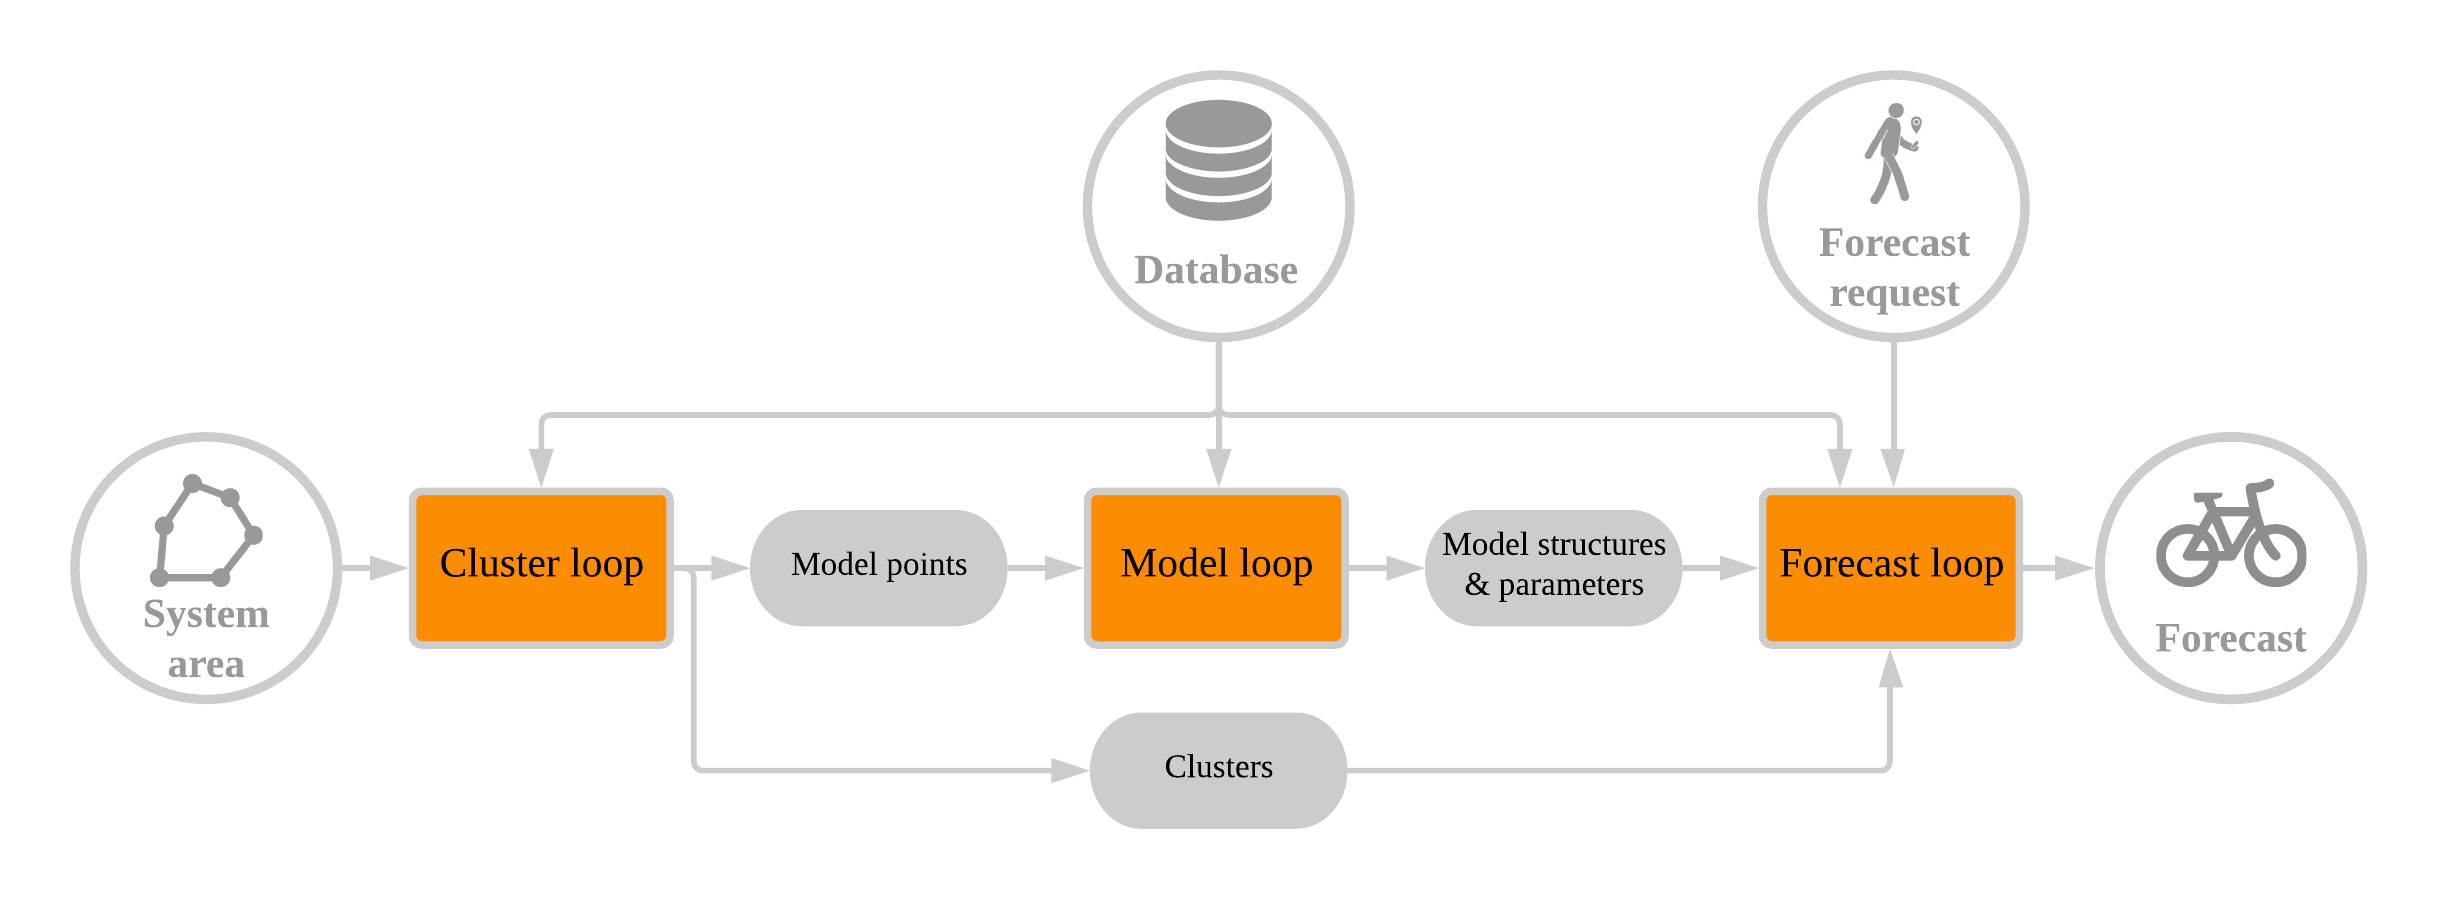
\includegraphics[width=\textwidth]{Figures/Workflow} \caption{Overall design of DBAFS}\label{fig:overalldesign}
\end{figure}
\section{Software}\label{software}

The underlying code of DBAFS (see Appendix A) is written in the R
programming language (R Core Team,
\protect\hyperlink{ref-rlanguage}{2013}). However, Structured Query
Language (SQL) statements are nested within the R code to retrieve data
from a PostgreSQL database (PostgreSQL,
\protect\hyperlink{ref-postgres}{2014}), and to run some of the heavier
data pre-processing computations on the database server. These
computations are discussed in section 3.4.

On top of functions that are included in R by default, DBAFS uses of
several extensions, listed below.
\begin{itemize}
\tightlist
\item
  The \texttt{ClustGeo} package, for spatially constrained clustering
  (Chavent et al., \protect\hyperlink{ref-clustgeo}{2018}).
\item
  The \texttt{clValid} package, for calculating the Dunn Index (Brock,
  Pihur, Datta, \& Datta, \protect\hyperlink{ref-clValid}{2008}).
\item
  The \texttt{forecast} package, for building forecasting models,
  decomposing time series, and forecasting time series (Hyndman \&
  Khandakar, \protect\hyperlink{ref-forecast}{2008}).
\item
  The \texttt{lubridate} package, for processing dates and timestamps
  (Grolemund \& Wickham, \protect\hyperlink{ref-lubridate}{2011}).
\item
  The \texttt{RPostgreSQL} package, for connecting to a PostgreSQL
  database and running SQL code on the database server (Conway,
  Eddelbuettel, Nishiyama, Prayaga, \& Tiffin,
  \protect\hyperlink{ref-RPostgreSQL}{2017}).
\item
  The \texttt{sf} package, for processing spatial data (Pebesma,
  \protect\hyperlink{ref-sf}{2018}).
\item
  The \texttt{tsibble} package, for pre-processing time series datasets
  (E. Wang, Cook, \& Hyndman, \protect\hyperlink{ref-tsibble}{2018}).
\end{itemize}
\section{System area}\label{system-area}

Each dockless bike sharing system has a system area, in which the bikes
can be used. Usually, leaving a bike outside of the system area, will
result in a fine. DBAFS produces forecasts only inside the system area,
and therefore, the geographical outline of this area needs to be
provided. DBAFS accepts all filetypes that can be read with a driver
supported by the \texttt{st\_read} function in the \texttt{sf} package,
given that the included feature is either a polygon or multipolygon. The
accepted filetypes include, among others, ESRI shapefiles, GeoPackage
files and GeoJSON files. It is also possible to retrieve the feature
from a PostgreSQL database.

\section{Database}\label{database}

In a dockless bike sharing system, each bike is equipped with a Global
Positioning System (GPS). Every \(i_{d}\) minutes, the geographical
locations of all bikes are saved into a database, together with the
corresponding timestamp. The locations of the bikes that are not in use
at the current time, and thus available, are usually visible to the
users of the system in a mobile application, and stored separately from
the data regarding bikes that are in use.

The geographical location of a bike is spatial data, and should be
stored as such. An advanced and open source database management system
for spatial data is PostgreSQL in combination with the PostGIS
extension. DBAFS requires the data to be stored in such a database, and
to have a sub-daily temporal resolution. Each feature represents the
location of an available bike at a certain timestamp and should at least
have the following fields.
\begin{itemize}
\tightlist
\item
  A timestamp of data type \texttt{timestamp\ with\ time\ zone}.
\item
  A geographical location of data type \texttt{geometry(Point)}.
\item
  A unique ID of the bike to which the feature belongs.
\end{itemize}
Data are pre-processed on the database server, and only the data that
are needed, are loaded into memory. In DBAFS, this pre-processing step
involves two different procedures. The first one leads to data that
contain information about the distance to the nearest bike for several
timestamps in the past, and is discussed in the next sub-section, while
the latter produces a dataset with all the bicycle pick-ups in the
database, and is discussed in section 3.3.2.

\subsection{Distance data}\label{distance-data}

For a given location, the distance from that location to the nearest
available bike is calculated for each timestamp \(t \in T\), where \(T\)
is a regularly spaced time interval containing timestamps within the
timespan of the historical data. The temporal resolution of \(T\) equals
\(i_{s}\) minutes, where \(i_{s} \geq i_{d}\). The nearest available
bike is found by a nearest neighbour searching process that uses spatial
indices on the geometries. In practice, this means that it is not needed
to first compute the distances to all available bikes, which would slow
down the process vastly. If no bike can be found, for example due to a
server error at that timestamp, or the unlikely event that there are no
bikes available anywhere in the system, the corresponding feature will
be inserted in the data, with a non-available distance value, \(NA\).
That is, after pre-processing, the resulting time series will always be
regular, with all timestamps \(t \in T\) present. This also means that
when data are queried for several locations at the same times, the
resulting time series will always have the same length.

The calculated distances are great-circle distances assuming a spherical
earth a radius equal to the mean radius of the WGS84 ellipsoid, as
showed in Equation 3.1.

\[
L_{AB} = \frac{(2a+b)}{3} \times
\frac{\pi}{180} \times
arccos(sin\phi_{A}sin\phi_{B}+cos\phi_{A}cos\phi_{B}cos\Delta\lambda)
\]

Where \(L_{AB}\) is the great-circle distance between point \(A\) and
point \(B\) in meters, \(\phi_{A}\) and \(\phi_{B}\) are the latitudes
of respectively point \(A\) and \(B\) in degrees on the WGS84 ellipsoid,
and \(\Delta\lambda\) is the difference in longitude between the two
points, i.e. \(\lambda_{B}-\lambda_{A}\), in degrees on the WGS84
ellipsoid. Furthermore, \(a\) is the equatorial radius of the WGS84
ellipsoid in meters, which is defined to be \(6378137\), and \(b\) is
the polar radius of the WGS84 ellipsoid in meters, which is defined to
be \(6378137 \times (1 - 298.257 223 563^{-1}) = 6 356 752.3142\)
(Iliffe \& Lott, \protect\hyperlink{ref-iliffe2008}{2008}).

The sphere is chosen since calculating distances on the ellipsoid itself
slows down computations, and, on the geographical scale of a dockless
bike sharing system, has an accuracy gain that can be neglected. Working
with the shortest distance over the street network might in most cases
be more appropriate, but at the same time involves much more complex
computations, especially when either the given location or the locations
of the bikes are not exactly on the network lines.

The output of this pre-processing operation is a time series with \(T\)
features and a temporal resolution of \(i_{s}\), belonging to one single
location in the system area of the dockless bike sharing system. Each
feature contains a timestamp and the great-circle distance from the
given location to the nearest available bike in meters. Such data are
referred to in this thesis as \emph{distance data}.

\subsection{Usage data}\label{usage-data}

A pick-up is the moment that a user of the dockless bike sharing system
unlocks a bike to make a trip. For the historical database containing
the locations of the available bikes, this means that the bike that is
picked-up will be present in the data at the last timestamp before the
pick-up, but missing at the first timestamp after the pick-up. In DBAFS,
this is used to retrieve all the pick-ups from the database. Historical
data with the highest possible temporal resolution, i.e. \(i_{d}\)
minutes, are queried for one single bike ID. Then, all timestamps that
are missing, are added to the data, but without an available location.
If feature \(j\) has an available location, but feature \(j+1\) has not,
\(j\) is considered a pick-up. This procedure is repeated for all
individual bikes. If more than 20\% of the features within the same
minute are considered pick-ups, it is assumed that this was caused by a
server error, and they are removed from the data.

The output of this pre-processing operation is a data frame with all the
features in the database that are considered pick-ups. Each feature has
at least a timestamp, a geographical location and a bike ID. The number
of pick-ups in an area represents the usage intensity of the bike
sharing system. Such data are therefore referred to in this thesis as
\emph{usage data}.

Obviously, the procedure described in this sub-section has some
deficiencies. The removal of a bike by the system operator, for
redistribution or maintenance purposes, is falsely considered to be a
pick-up. Specific information about redistribution patterns can be
added, but will in many cases be unavailable, and even if available,
those patterns may be too irregular to implement adequately in the
workflow. However, in DBAFS, the usage data are only used to define the
location of the model point in a cluster, and not to analyze usage
patterns into detail. Therefore, fully accurate data are not
indispensable for this purpose, and the current procedure forms a
sufficient basis.

\section{Forecast request}\label{forecast-request}

A forecast request is made by a user. DBAFS assumes such a request to be
composed of the geographical coordinates of the location at which the
forecast should be made. The coordinates can be expressed in any
coordinate reference system that is included in the PROJ library
(PROJ-contributors, \protect\hyperlink{ref-proj}{2018}). The timestamp
can be expressed in any time zone that is included in the Time Zone
database (Eggert \& Olson, \protect\hyperlink{ref-tz}{2018}).

\section{Cluster loop}\label{cluster-loop}

The main purpose of the cluster loop is to find suitable locations for
the model points. The loop starts by laying a grid with square cells of
\(p \times p\) meters over the system area of the dockless bike sharing
system, such that each location in the system area is part of one of
those grid cells. Then, the geographical coordinates of the centroids of
the grid cells are calculated, and \(m_{c}\) weeks of distance data are
queried for each of those centroids.

The result of this query operation is a set of \(n\) time series, where
\(n\) is the number of cells in the overlaying grid. To reduce the
dimensionality of the clustering task, each of those time series is
simplified by averaging its values per hour of the week. This is
followed by a min-max normalization, such that time series that show the
same patterns over time, but with different means, will be considered
similar. The normalized values are calculated with Equation 3.2.

\[ \hat{y_{t}} = \frac{y_{t} - y_{min}}{y_{max} - y_{min}} \]

Where \(\hat{y_{t}}\) is the normalized value of \(y_{t}\), \(y_{min}\)
is the minimum value in the time series, and \(y_{max}\) is the maximum
value in the time series. By definition, \(0 \leq \hat{y_{t}} \leq 1\).

For all possible combinations of the \(n\) averaged, normalized time
series, a dissimilarity value is calculated based on the Euclidean
distance between the two series, as defined in Equation 2.x. Since all
time series have the same length, and observations at the same
timestamps, the Euclidean approach is appropriate, and for the sake of
simplicity, chosen over dynamic time warping. Furthermore, since
out-of-phase similarities are ignored, areas where similar peaks and
valleys in the data occur at different times of the week, will be
grouped into different clusters, which gives a better representation of
the spatio-temporal dynamics of the bike sharing system.

All Euclidean dissimilarity values are stored together in a
\(n \times n\) matrix and form the time series dissimilarity matrix
\(A\). At the same time, a spatial dissimilarity matrix \(B\) is
created. This matrix is equal to \(1-C\), where \(C\) is the adjacency
matrix of the \(n\) grid cells. That is, \(B\) is a \(n \times n\)
matrix in which \(b_{i,j} = 0\) when grid cells \(i\) and \(j\) are
neighbours, and \(b_{i,j} = 1\) otherwise.

\(A\) and \(B\) are used as the dissimilarity matrices of respectively
the feature space and the constraint space in a spatially constrained
hierarchical clustering procedure, which was introduced in section
2.5.3. Before the final clustering procedure can start, the number of
clusters \(k\) and the value of the mixing parameter \(\alpha\) need to
be set. DBAFS does this based on the approach proposed by Chavent et al.
(\protect\hyperlink{ref-clustgeo}{2018}), which was discussed in section
2.5.3, but replaces the manual interpretation of plots by a fully
automated method, as described below.

At first, only the dissimilarity values in the feature space are
clustered, i.e.~a spatially constrained hierarchical clustering with
\(\alpha = 0\) is performed, which results in a sequence of partitions
\{\(\Lambda_{k}\)\}. For each \(k \in K\), where \(K\) is a finite set
of strictly positive integers, the Dunn Index \(V(\Lambda_{k})\) of a
specific partition \(\Lambda_{k}\) is calculated with Equation 2.x.
Then, the value of \(k\) that maximizes \(V(\Lambda_{k})\) is chosen as
the optimal value of \(k\), and is referred to as \(k^{*}\).

Secondly, for each \(\omega \in \Omega\), where \(\Omega =\)
\{\(0, 0.1, 0.2, ..., 1\)\}, a spatially constrained hierarchical
clustering with \(k = k^{*}\) and \(\alpha = \omega\) is performed,
which results in a set of partitions \{\(\Lambda_{\omega}\)\}, of the
same length as \(\Omega\). For each partition \(\Lambda_{\omega}\), the
sum \(\sum I_{f}(C_{i}^{\omega})\) and the sum
\(\sum I_{c}(C_{i}^{\omega})\) are calculated, where \(C_{i}^{\omega}\)
are the clusters in \(\Lambda_{\omega}\), \(I_{f}\) is the information
criterion regarding the feature data (i.e.~the first part of Equation
2.x) and \(I_{c}\) is the information criterion regarding the constraint
data (i.e.~the second part of Equation 2.x). Then, the value of
\(\omega\) that maximizes \(\sum I_{c}(C_{i}^{\omega})\), given that
\(\big((\sum I_{f}(C_{i}^{\omega}) / \sum I_{f}(C_{i}^{0})\big) \geq 0.9\),
is chosen as the optimal value of \(\alpha\), and referred to as
\(\alpha^{*}\). That is, clusters are made as spatially contiguous as
possible, with the restriction that this can never lead to an
information loss in the feature space of more than 10\%.

With \(A\), \(B\), \(k^{*}\) and \(\alpha^{*}\) set, the final spatially
constrained hierarchical clustering is performed. The output of this
procedure is a single partition, in which all time series are grouped
into a cluster. Some extra restrictions are imposed subsequently. Since
the spatial constraint was not strict, it is not guaranteed that all the
clusters in this partition are fully spatially contiguous. Clusters
consisting of more than one set of spatially connected grid cells, can
occur in situations where striving for full spatial contiguity would
lead to a too large information loss in the feature space, and thus,
clusters that would not truly represent areas with similar patterns in
the distance data. In such cases, all spatially contiguous areas in
these clusters, will be treated as seperate clusters, with their own
model point. However, this may lead to a high number of model points
that each represent a very small area. When this area has a high usage
intensity, the described situation is acceptable. When this area has a
very low usage intensity, on the other hand, it is unwanted to have a
seperate model point representing it. Therefore, whenever a cluster has
a usage intensity of less than two bicycle pick-ups per day, it will be
merged with the closest neighbouring cluster. which is found by
minimizing the inter-centroid distance.

Now, each cluster is guaranteed to be spatially contiguous, and gets
assigned one model point. Before the locations for the model points are
chosen, usage data is queried from the database, and the total number of
pick-ups is calculated for each grid cell. This number is assigned as a
variable to the corresponding grid cell centroids. Then, for each
cluster, the arithmetic means of the coordinates of all grid cell
centroids in that cluster, are calculated, weighted by the number of
pick-ups. Equation 3.3 shows the calculation of the weighted average
latitude of a cluster, while Equation 3.4 shows the calculation of the
weighted average longitude of a cluster.

\[ \phi^{*} = \frac{\sum_{i=1}^{m} \phi_{i} \times p_{i}}{\sum_{i=1}^{m} p_{i}} \]
\[ \lambda^{*} = \frac{\sum_{i=1}^{m} \lambda_{i} \times p_{i}}{\sum_{i=1}^{m} p_{i}} \]

Where \(\phi^{*}\) and \(\lambda^{*}\) are respectively the weighted
average latitude and the weighted average longitude of the cluster,
\(\phi_i\) and \(\lambda_{i}\) are respectively the latitude and
longitude of the \(i_{th}\) grid cell centroid in the cluster, \(p_{i}\)
is the number of pick-ups in the \(i_{th}\) grid cell in the cluster,
and \(m\) is the total number of grid cells in the cluster.

The combination \{\(\phi^{*}, \lambda^{*}\)\} forms the coordinate pair
of the weighted centroid of the cluster. This weighted centroid is then
chosen to be the model point of that cluster. In this way, a model point
is a cluster centroid which is dragged towards the areas where the usage
intensity of the bike sharing system is higher, and where accurate
forecasts are thus more important. The model points of all clusters are
send to the model loop. Finally, for each cluster, grid cells are first
dissolved, and then clipped by the system area, to form one geographic
outline of that cluster. The geographic outlines of all clusters, stored
as polygons, are send to the forecast loop. The complete methodology of
the cluster loop as described above is summarized in Figure 3.2.
\begin{figure}[h]
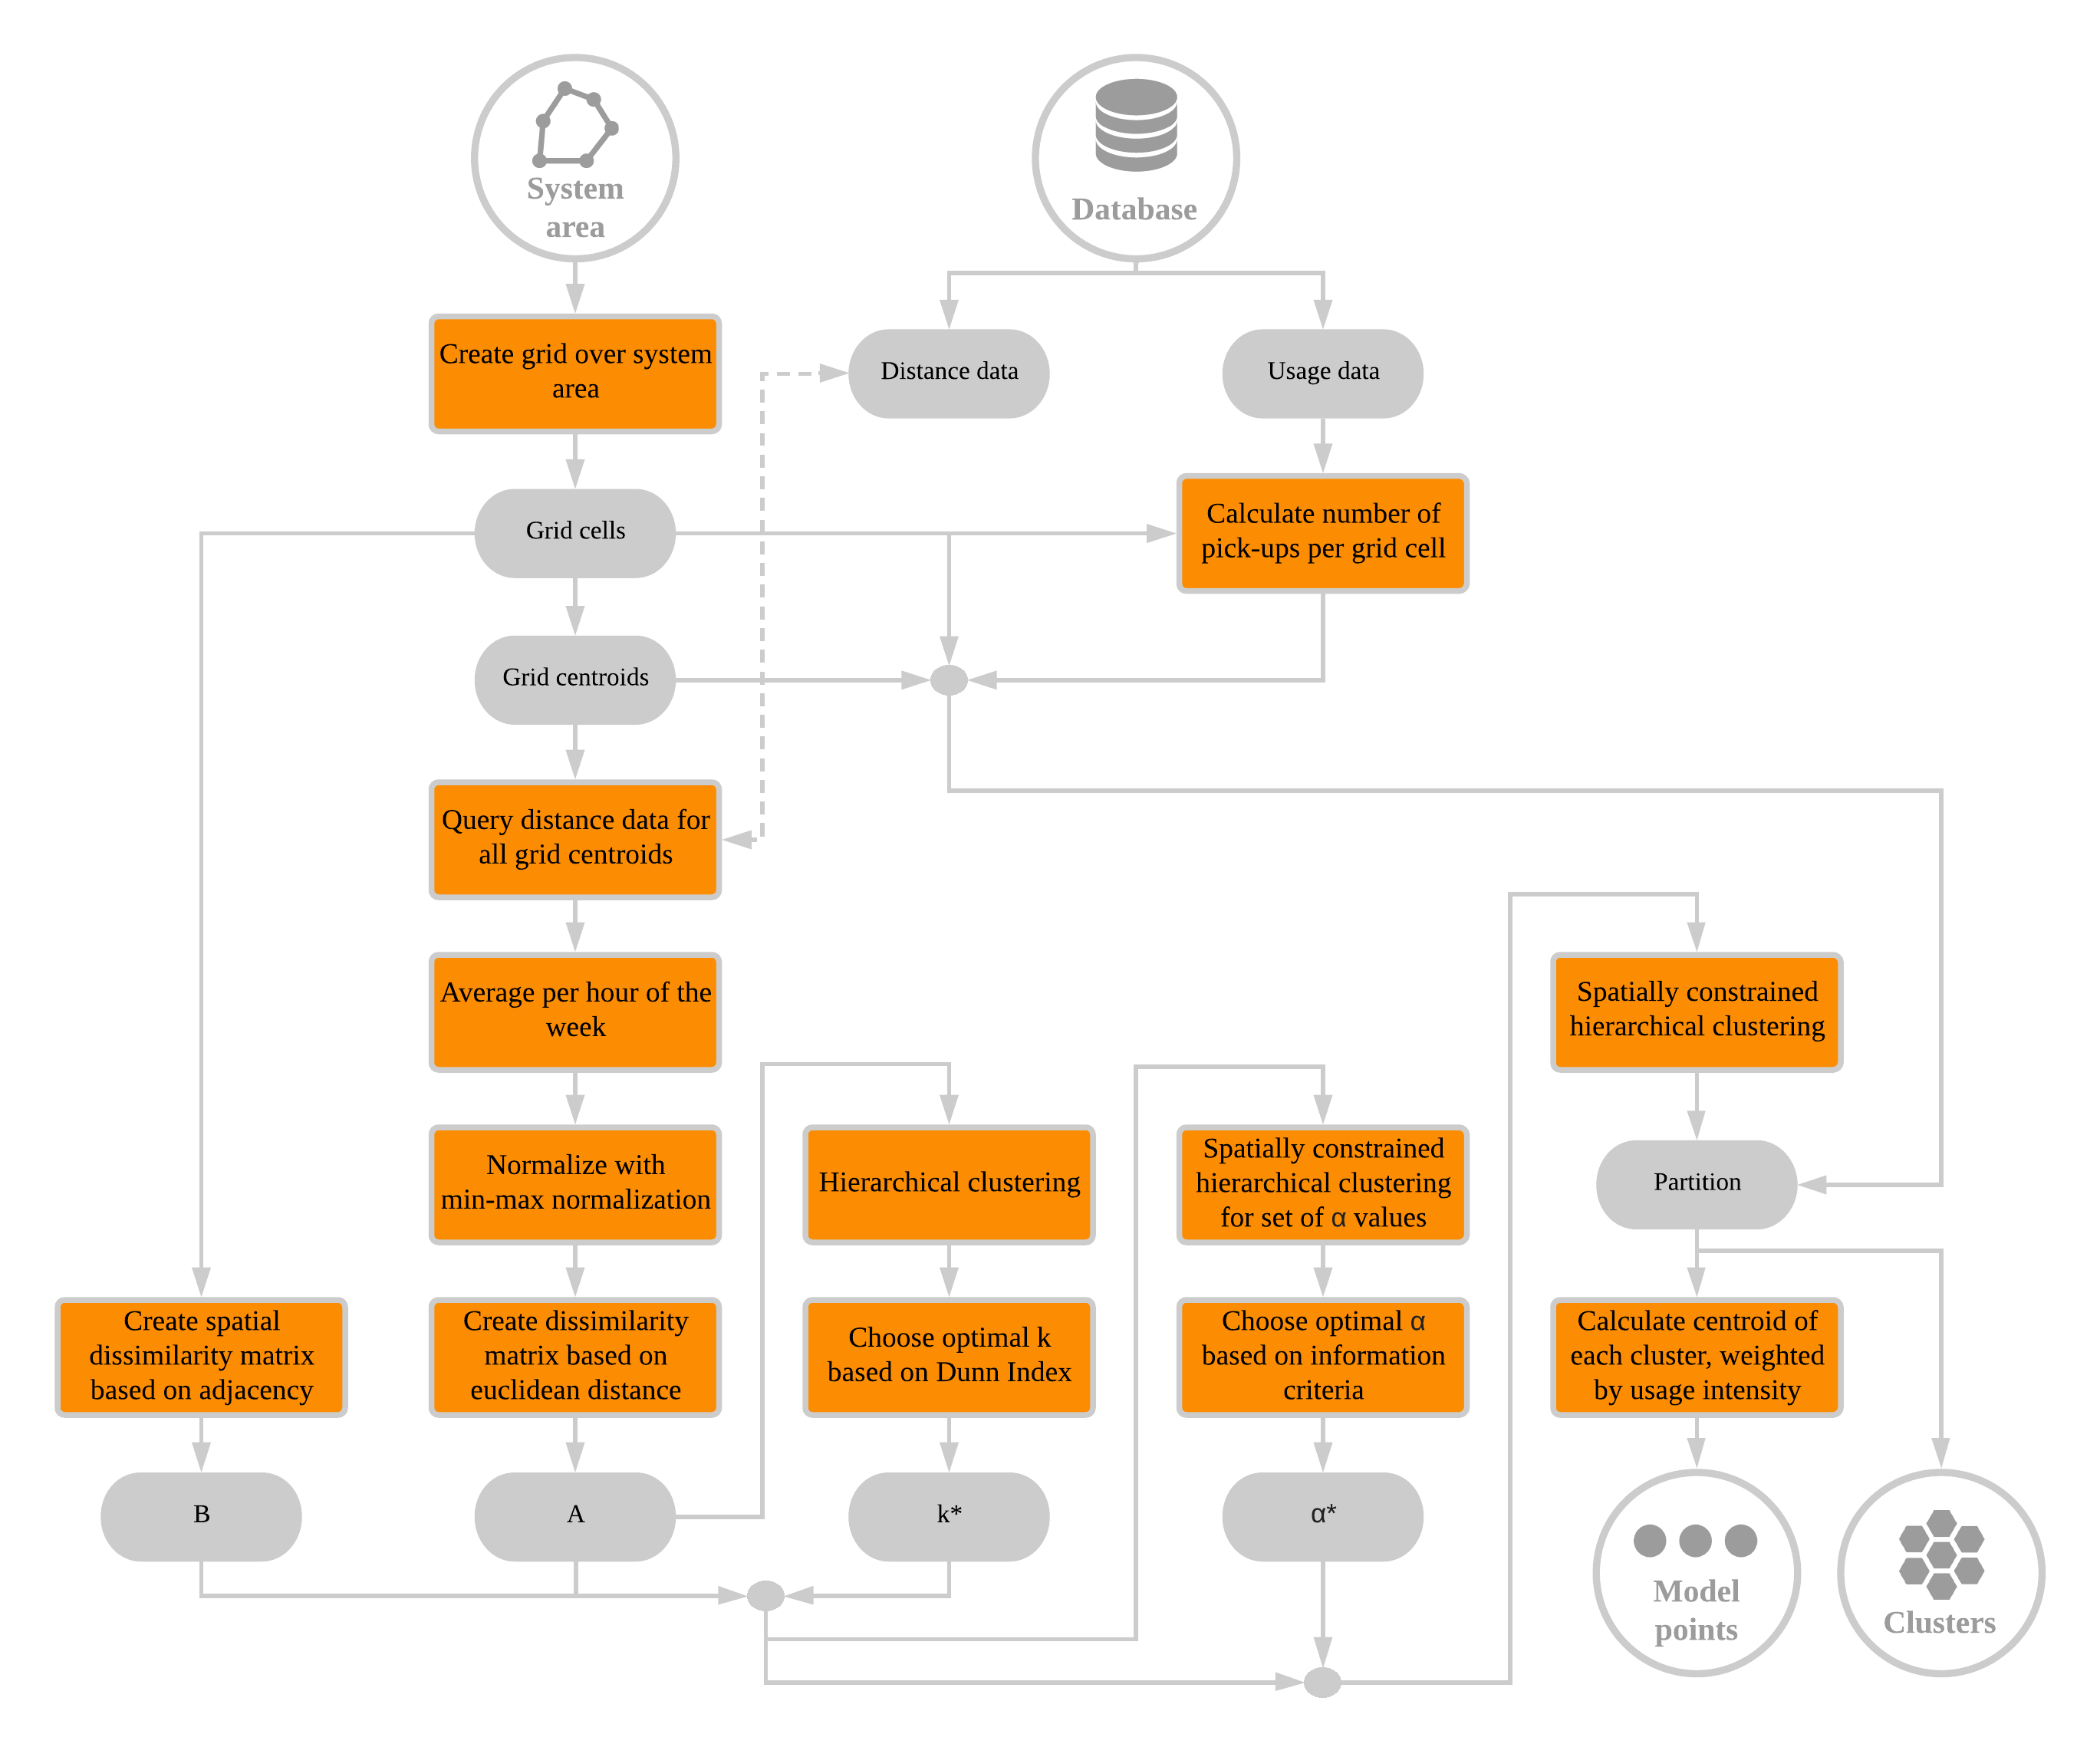
\includegraphics[width=\textwidth]{Figures/Clusterloop} \caption{Methodology of the cluster loop}\label{fig:clusterloop}
\end{figure}
\section{Model loop}\label{model-loop}

The main purpose of the model loop is to fit time series models to the
historical data of a limited set of geographical locations. These
locations are called the \emph{model points}, and result from a previous
pass through the cluster loop. For each model point, \(m_{m}\) weeks of
distance data are queried. All data are log-transformed, to stabilize
the variance, and to make sure that, when using the models for
forecasting, the forecasted distances will always be larger than zero.

If the data are seasonal, they will pass through the decomposition
process sequence. There, they will be decomposed into a trend, seasonal
and remainder component with STL, as introduced in section 2.3.3. Single
seasonal data, with either a daily or a weekly seasonal pattern, will be
decomposed once. Multiple seasonal data, that show both a daily and a
weekly seasonal pattern, will first be decomposed assuming that only
daily seasonality is present, after which the trend and remainder
component are added together, and decomposed again, now assuming weekly
seasonality. Hence, such data are eventually decomposed in a trend,
remainder and two seasonal components. Since STL is performed on the log
transformation of the original data, this indirectly implies that the
original data are decomposed in a multiplicative way, as explained at
the end of section 2.3.3.

STL requires a set of parameters to be defined in advance. For most of
them, there exist clear guidelines for the choice of their values,
indited by R. B. Cleveland et al.
(\protect\hyperlink{ref-cleveland1990}{1990}). Below, all STL parameters
are listed, including their quantification as used in DBAFS.
\begin{itemize}
\tightlist
\item
  \(n_{p}\), the number of observations per seasonal cycle. When
  decomposing assuming daily seasonality,
  \(n_{p} = 60 \times 24 / i_{s}\), and when assuming weekly
  seasonality, \(n_{p} = 60 \times 24 \times 7 / i_{s}\).
\item
  \(n_{i}\), the number of passes through the inner loop within one pass
  through the outer loop. It should be chosen large enough such that the
  updating of the seasonal and trend components converges. R. B.
  Cleveland et al. (\protect\hyperlink{ref-cleveland1990}{1990}) show
  that this convergence happens very fast, and that, inside a pass
  through the outer loop, only one pass through the inner loop is
  already sufficient. Hence, in DBAFS, \(n_{i} = 1\).
\item
  \(n_{o}\), the number of passes through the outer loop. To have near
  certainty of convergence, R. B. Cleveland et al.
  (\protect\hyperlink{ref-cleveland1990}{1990}) recommend ten passes
  through the outer loop. In R, to be extra safe, the default is set to
  fifteen passes. This will not be changed in DBAFS, hence
  \(n_{o} = 15\).
\item
  \(n_{s}\), the seasonal smoothing parameter. It should be chosen large
  enough to avoid overfitting, but small enough to allow slight
  variations over time. The choice of \(n_{s}\) is the only one where R.
  B. Cleveland et al. (\protect\hyperlink{ref-cleveland1990}{1990})
  propose a manual approach, that involves a visual interpretation of
  the time series plot. For an automated process that decomposes several
  time series, this is problematic. Hyndman \& Athanasopoulos
  (\protect\hyperlink{ref-hyndman2018fpp}{2018}), however, argue that a
  value of thirteen usually gives a good balance between overfitting and
  allowing slight variations. In DBAFS, their recommendation is used.
  Hence, \(n_{s} = 13\).
\item
  \(n_{l}\), the low-pass filter smoothing parameter. R. B. Cleveland et
  al. (\protect\hyperlink{ref-cleveland1990}{1990}) show that \(n_{l}\)
  always can be set equal to the least odd integer greater than or equal
  to \(n_{p}\), which is done in DBAFS as well.
\item
  \(n_{t}\), the trend smoothing parameter. It should be chosen large
  enough such that seasonal variation does not end up in the trend
  component, but small enough such that low-frequency effects do not end
  up in the remainder component. To achieve this goals, R. B. Cleveland
  et al. (\protect\hyperlink{ref-cleveland1990}{1990}) show that
  \(n_{t}\) should be chosen to be the smallest odd integer that
  satisfies the inequality \(n_{t} \geq 1.5n_{p} / (1-1.5n_{s}^{-1})\).
  In DBAFS, this is done as well.
\end{itemize}
Once the data are decomposed in a trend component, a remainder component
and one or two seasonal components, the trend and remainder are added
together, and send to the ARIMA process sequence. This part of the data
can be seen as the log-transformed, deseasonalized original data, and
should not contain seasonal patterns anymore. Data that were originally
already non-seasonal, skip the decomposition process sequence
completely, and are send to the ARIMA process sequence directly after
the log transformation. Both types are from now on referred to as the
\emph{non-seasonal data}.

In the ARIMA process sequence, an ARIMA(\(p\), \(d\), \(q\)) model is
fitted to the non-seasonal data, by applying the Hyndman-Khandakar
algorithm, as described in section 2.4.2.2. In R, the Hyndman-Khandakar
algorithm is implemented in the \texttt{auto.arima} function from the
\texttt{forecast} package, with the extra restriction that the order of
differencing \(d\) is not allowed to be larger than two. It also allows
missing values, by handling them exactly. This is an important
characteristic, since it means that models will be fitted even if some
observations are missing due to server errors.

To determine if the data of a model point should pass through the
decomposition process sequence, and if yes, how many seasonal components
should be subtracted, it is necessary to first identify the seasonal
patterns in the data. This is done with a variation on what Hyndman \&
Athanasopoulos (\protect\hyperlink{ref-hyndman2018fpp}{2018}) refer to
as \emph{time series cross-validation}, and works as follows. Four
different seasonality options are considered: no seasonality, only daily
seasonality, only weekly seasonality, and both daily and weekly
seasonality.

Then, the first two of the \(n_{w}\) weeks of data are selected and
log-transformed. Four different models are fitted to these data, each
assuming a different seasonality option. That is, when the option of no
seasonality is considered, the data are directly inputted into the ARIMA
process sequence. When one of the other options is considered, the data
first pass through the decomposition process sequence, and then, the
deseasonalized data are inputted into the ARIMA process sequence.
Subsequently, each day in the first week following the `model building
weeks', is forecasted separately. For the first day, this simply means
that the non-seasonal data on which the ARIMA(\(p\), \(d\), \(q\)) model
is build, are forecasted \(60 \times 24 / i_{s}\) time lags ahead. If
present, the seasonal component is forecasted in a naïve way, and added
to each result. For the second day, however, one extra day of data is
added, and the same ARIMA(\(p\),\(d\),\(q\)) model is used to forecast
the non-seasonal part of this extended data \(60 \times 24 / i_{s}\)
time lags ahead, and if present, the naïve seasonal forecasts are added
to the results. This process repeats for all seven days, each time using
one extra day of data.

Once all days in this `forecasting week' are forecasted, the two weeks
of data on which the models were build, are now extended by one week of
new data. On this three-week dataset, new models are build for each of
the four seasonality options, and again, each day in the next week is
forecasted separately. This shifting of the model building period keeps
repeating, until there are no more weeks left to forecast. Then, for
each of the seasonality options, the total RMSE of all forecasts is
calculated. The option with the lowest RMSE, is the identified seasonal
pattern of the data.

After the log-transformation, seasonality detection, possible
decomposition, and model building, the following output is obtained. All
model points have an ARIMA(\(p\), \(d\), \(q\)) model that describes the
non-seasonal part of their data. Additionally, the length of the
seasonal period in their data is known. This can either be a single
non-zero integer, in the case of only a daily or weekly seasonality, a
vector of two non-zero integers, in the case of both a daily and a
weekly seasonality, or zero, in the case of no seasonality. The chosen
values \(p\), \(d\) and \(q\) of the ARIMA model, the estimated
parameter values \(\hat\phi_{1},...,\hat\phi_{p}\) and
\(\hat\theta_{1},...,\hat\theta_{q}\) of the ARIMA model, and the
identified length of the seasonal period, \(L_{s}\), are all send to the
forecast loop. The complete methodology of the model loop as described
above is summarized in Figure 3.4.
\begin{figure}[H]
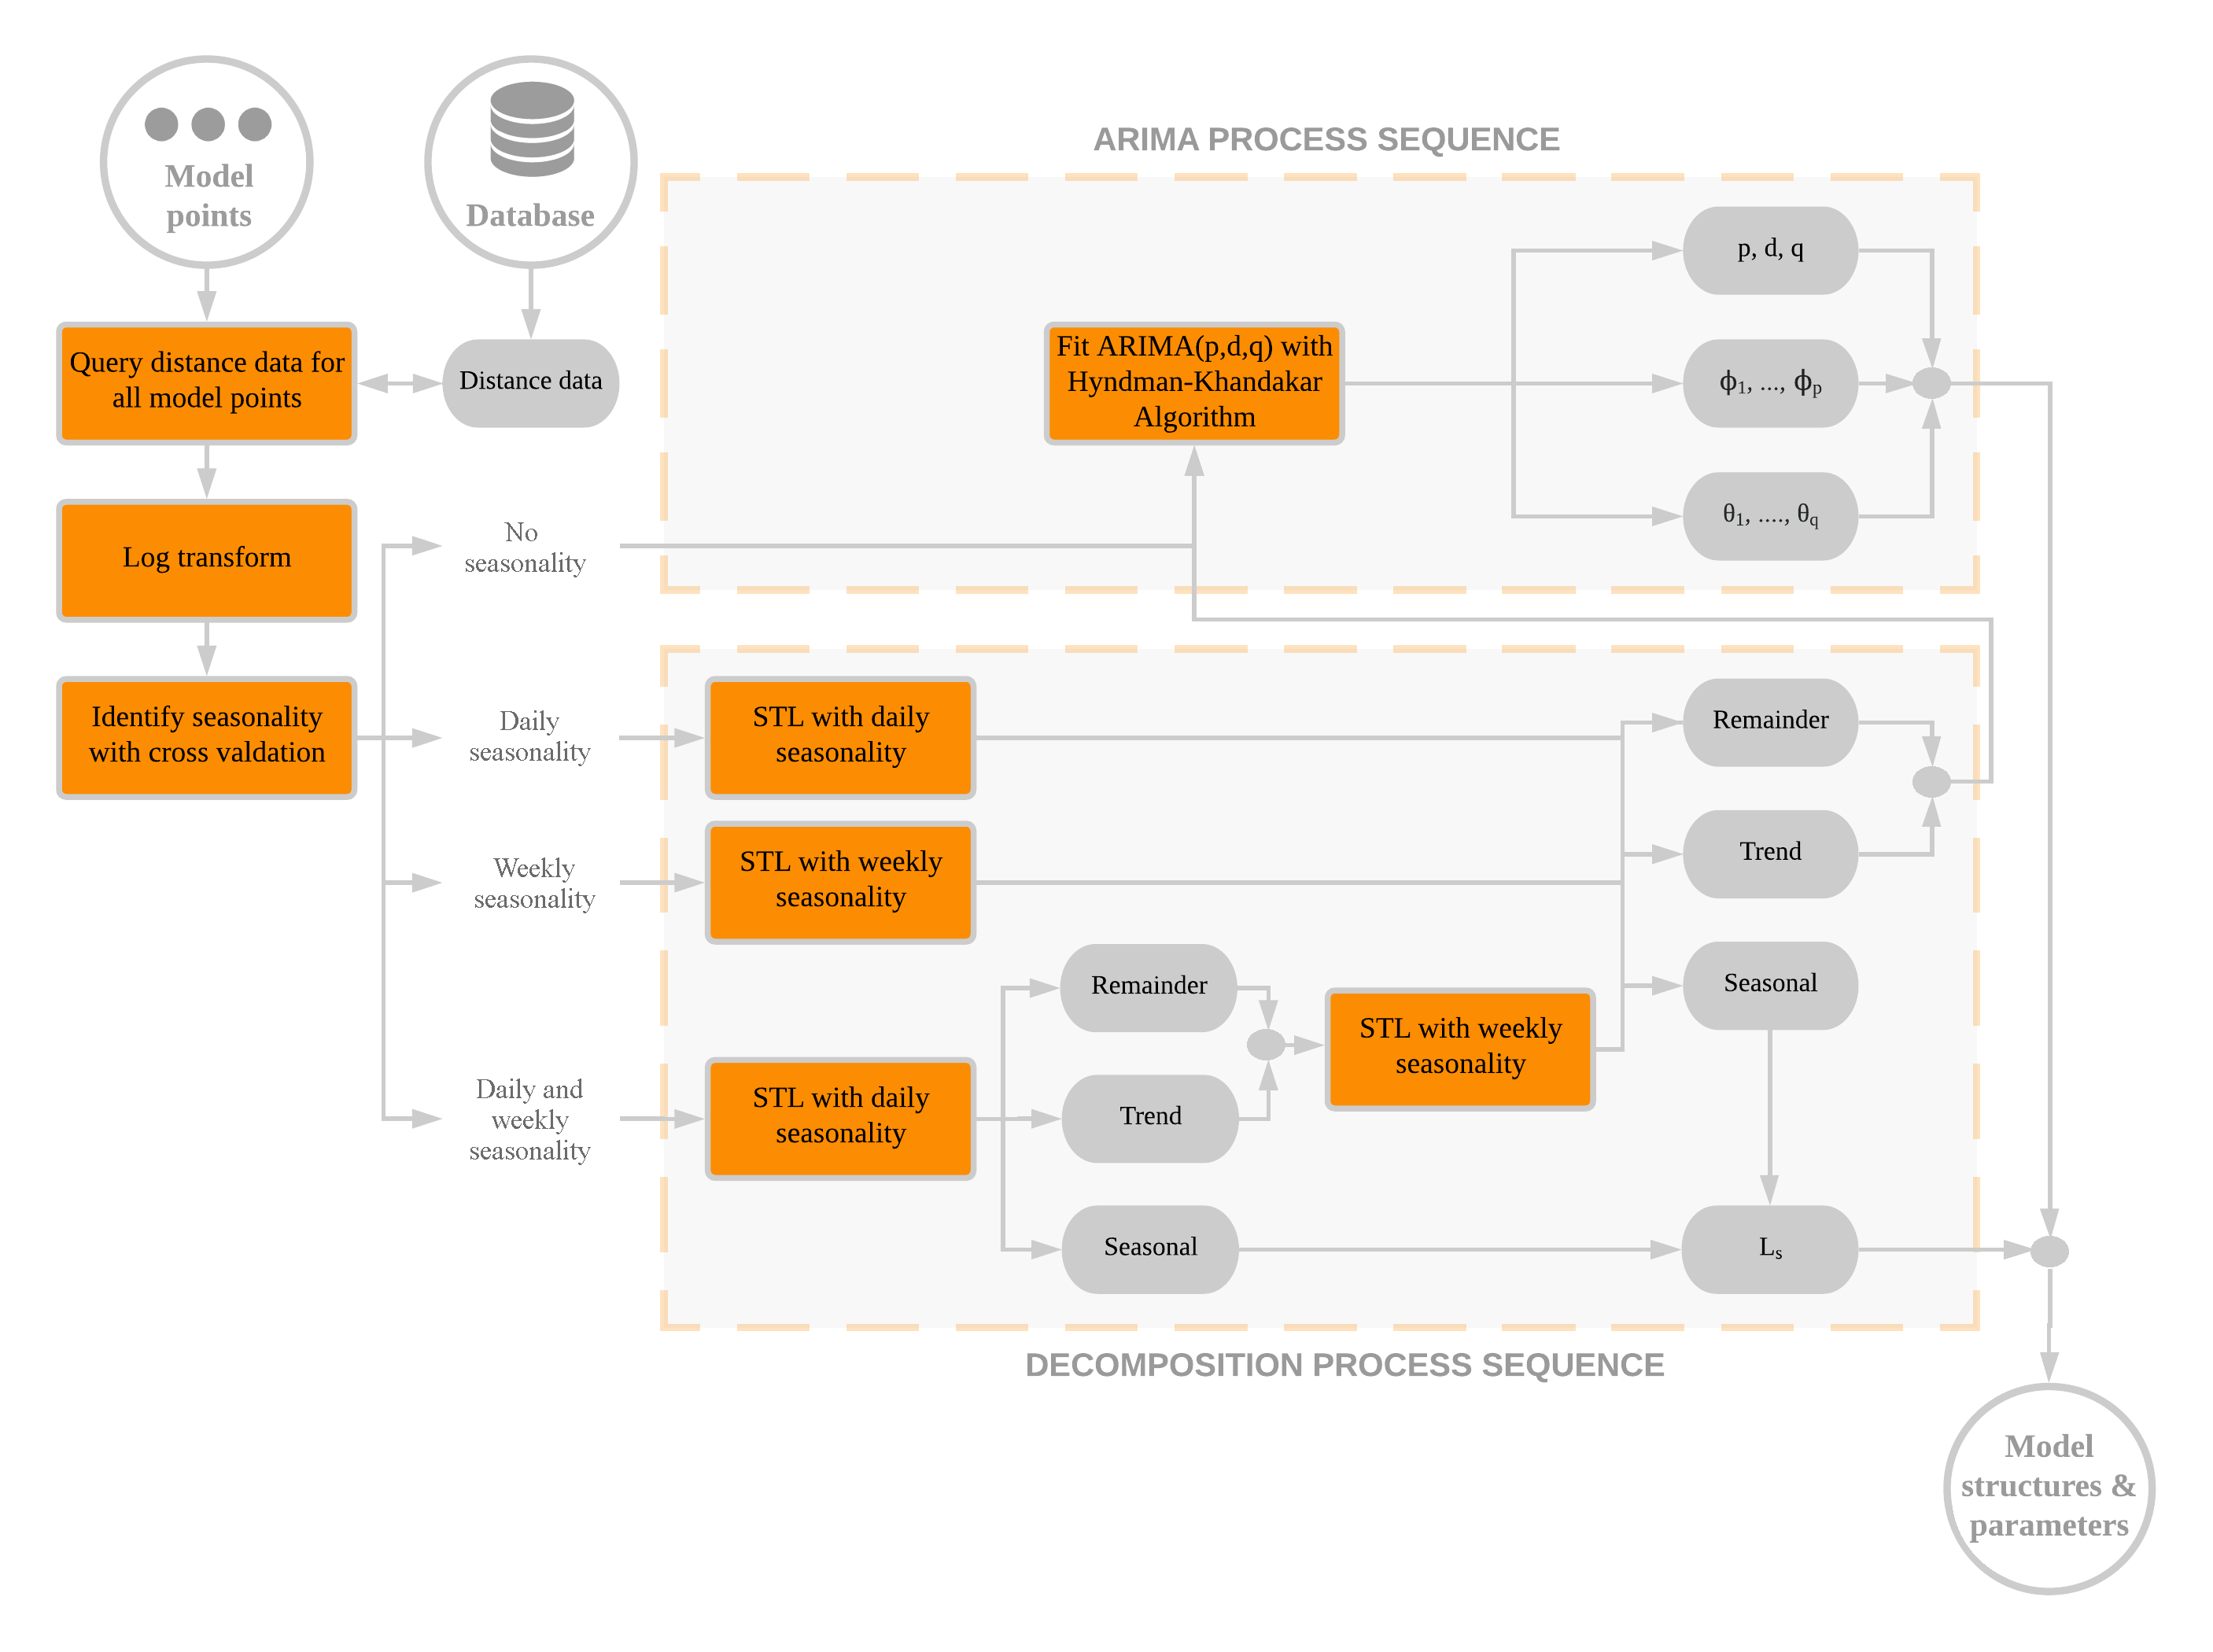
\includegraphics[width=\textwidth]{Figures/Modelloop} \caption{Methodology of the model loop}\label{fig:modelloop}
\end{figure}
\section{Forecast loop}\label{forecast-loop}

The main purpose of the forecast loop is to produce a forecast whenever
it is requested by a user. The forecasting task is split in two:
seasonal forecasts capture the seasonal patterns in the data, while an
ARIMA(\(p\), \(d\), \(q\)) model takes care of the short-term dynamics.
The geographical location that comes with such a forecast request, is
intersected with the clusters that resulted from a previous pass through
the cluster loop. This process returns the cluster in which the
requested forecast location lies. Subsequently, the model structure and
parameters from the model that belongs to this specific cluster, are
taken from a previous pass through the model loop. Since the clusters
represent areas with similar patterns in the data, but not necessarily
with similar means, the inherited model structure only provides the
length of the seasonal patterns, and not the values corresponding to
each season. Therefore, for the location of the forecast request,
\(m_{f}\) weeks of distance data are queried, which will be used for
seasonal decomposition, whenever the inherited model structure has an
identified seasonality. The length of these data should be at least
twice the length of the longest seasonal pattern, plus one observation.
For example, when a weekly seasonality is present in hourly data, the
data needed for forecasting should at least contain
\(24 \times 7 \times 2 + 1 = 337\) observations.

The queried distance data are log-transformed. Then, they are decomposed
by STL, using the identified seasonal period length(s) \(L_{s}\), which
is stored in the provided model structure. When \(L_{s} = 0\), this
decomposition step is skipped, and the data are treated in the same way
as the combination of trend and remainder that outputs from STL. Both
types are referred to as the \emph{non-seasonal data}. With the
ARIMA(\(p\), \(d\), \(q\)) model that was taken from the model loop, the
non-seasonal data are forecasted \(h\) time lags ahead.
\(h = (T_{f} - T_{c}) / i_{s}\), where \(i_{s}\) is the temporal
resolution of the pre-processed distance data, \(T_{c}\) is the
timestamp in the distance data that is closest to the time at which the
forecast request was send and \(T_{f}\) is the last timestamp in the
interval
\{\(T_{c}, T_{c} + i_{s}, T_{c} + 2i_{s}, T_{c} + 3i_{s}, ..., T_{c} + ki_{s} | T_{c} + ki_{s} \leq T_{r}\)\},
where \(T_{r}\), in turn, is the time for which the forecast is
requested. For example, the distance data contains values for each
quarter of an hour, the forecast request was send at 15:48, and the
forecast is requested for 16:40. Then, \(T_{c}\) will be 15:45, the last
timestamp in the queried distance data, and \(T_{f}\) will be 16:30, the
last quarterly hour timestamp before the requested forecast time. Hence,
\(h = 3\). That is, a forecast meant for 16:40, will in that case
effectively be a forecast for 16:30. The values of \(p\), \(d\), and
\(q\) in the ARIMA model are inherited from the model structure provided
by the model loop, just as the estimated parameter values
\(\hat\phi_{1},...,\hat\phi_{p}\) and
\(\hat\theta_{1},...,\hat\theta_{q}\).

For the data that were decomposed, the seasonal component is forecasted
separately. This is done with a seasonal naïve forecasting method, as
described in section 2.x. Then, the point forecast of the seasonal
component is added to the point forecast of the non-seasonal data, to
construct reseasonalized point forecast. The seasonal point forecast is
also added to the upper and lower bounds of the prediction intervals, to
construct reseasonalized prediction intervals. That is, the prediction
intervals of the non-seasonal data are shifted in line with the point
forecast, but do not get wider. Hence, the uncertainty of the seasonal
forecasts is not included in the final prediction intervals. This keeps
calculations simple, and is a reasonable approach, according to Hyndman
\& Athanasopoulos (\protect\hyperlink{ref-hyndman2018fpp}{2018}).

The forecasted distance to the nearest available bike, for the requested
time and location, together with the corresponding 95\% prediction
interval, forms the output of DBAFS, and is send back to the user. The
complete methodology of the forecast loop as described above is
summarized in Figure 3.5.
\begin{figure}[h]
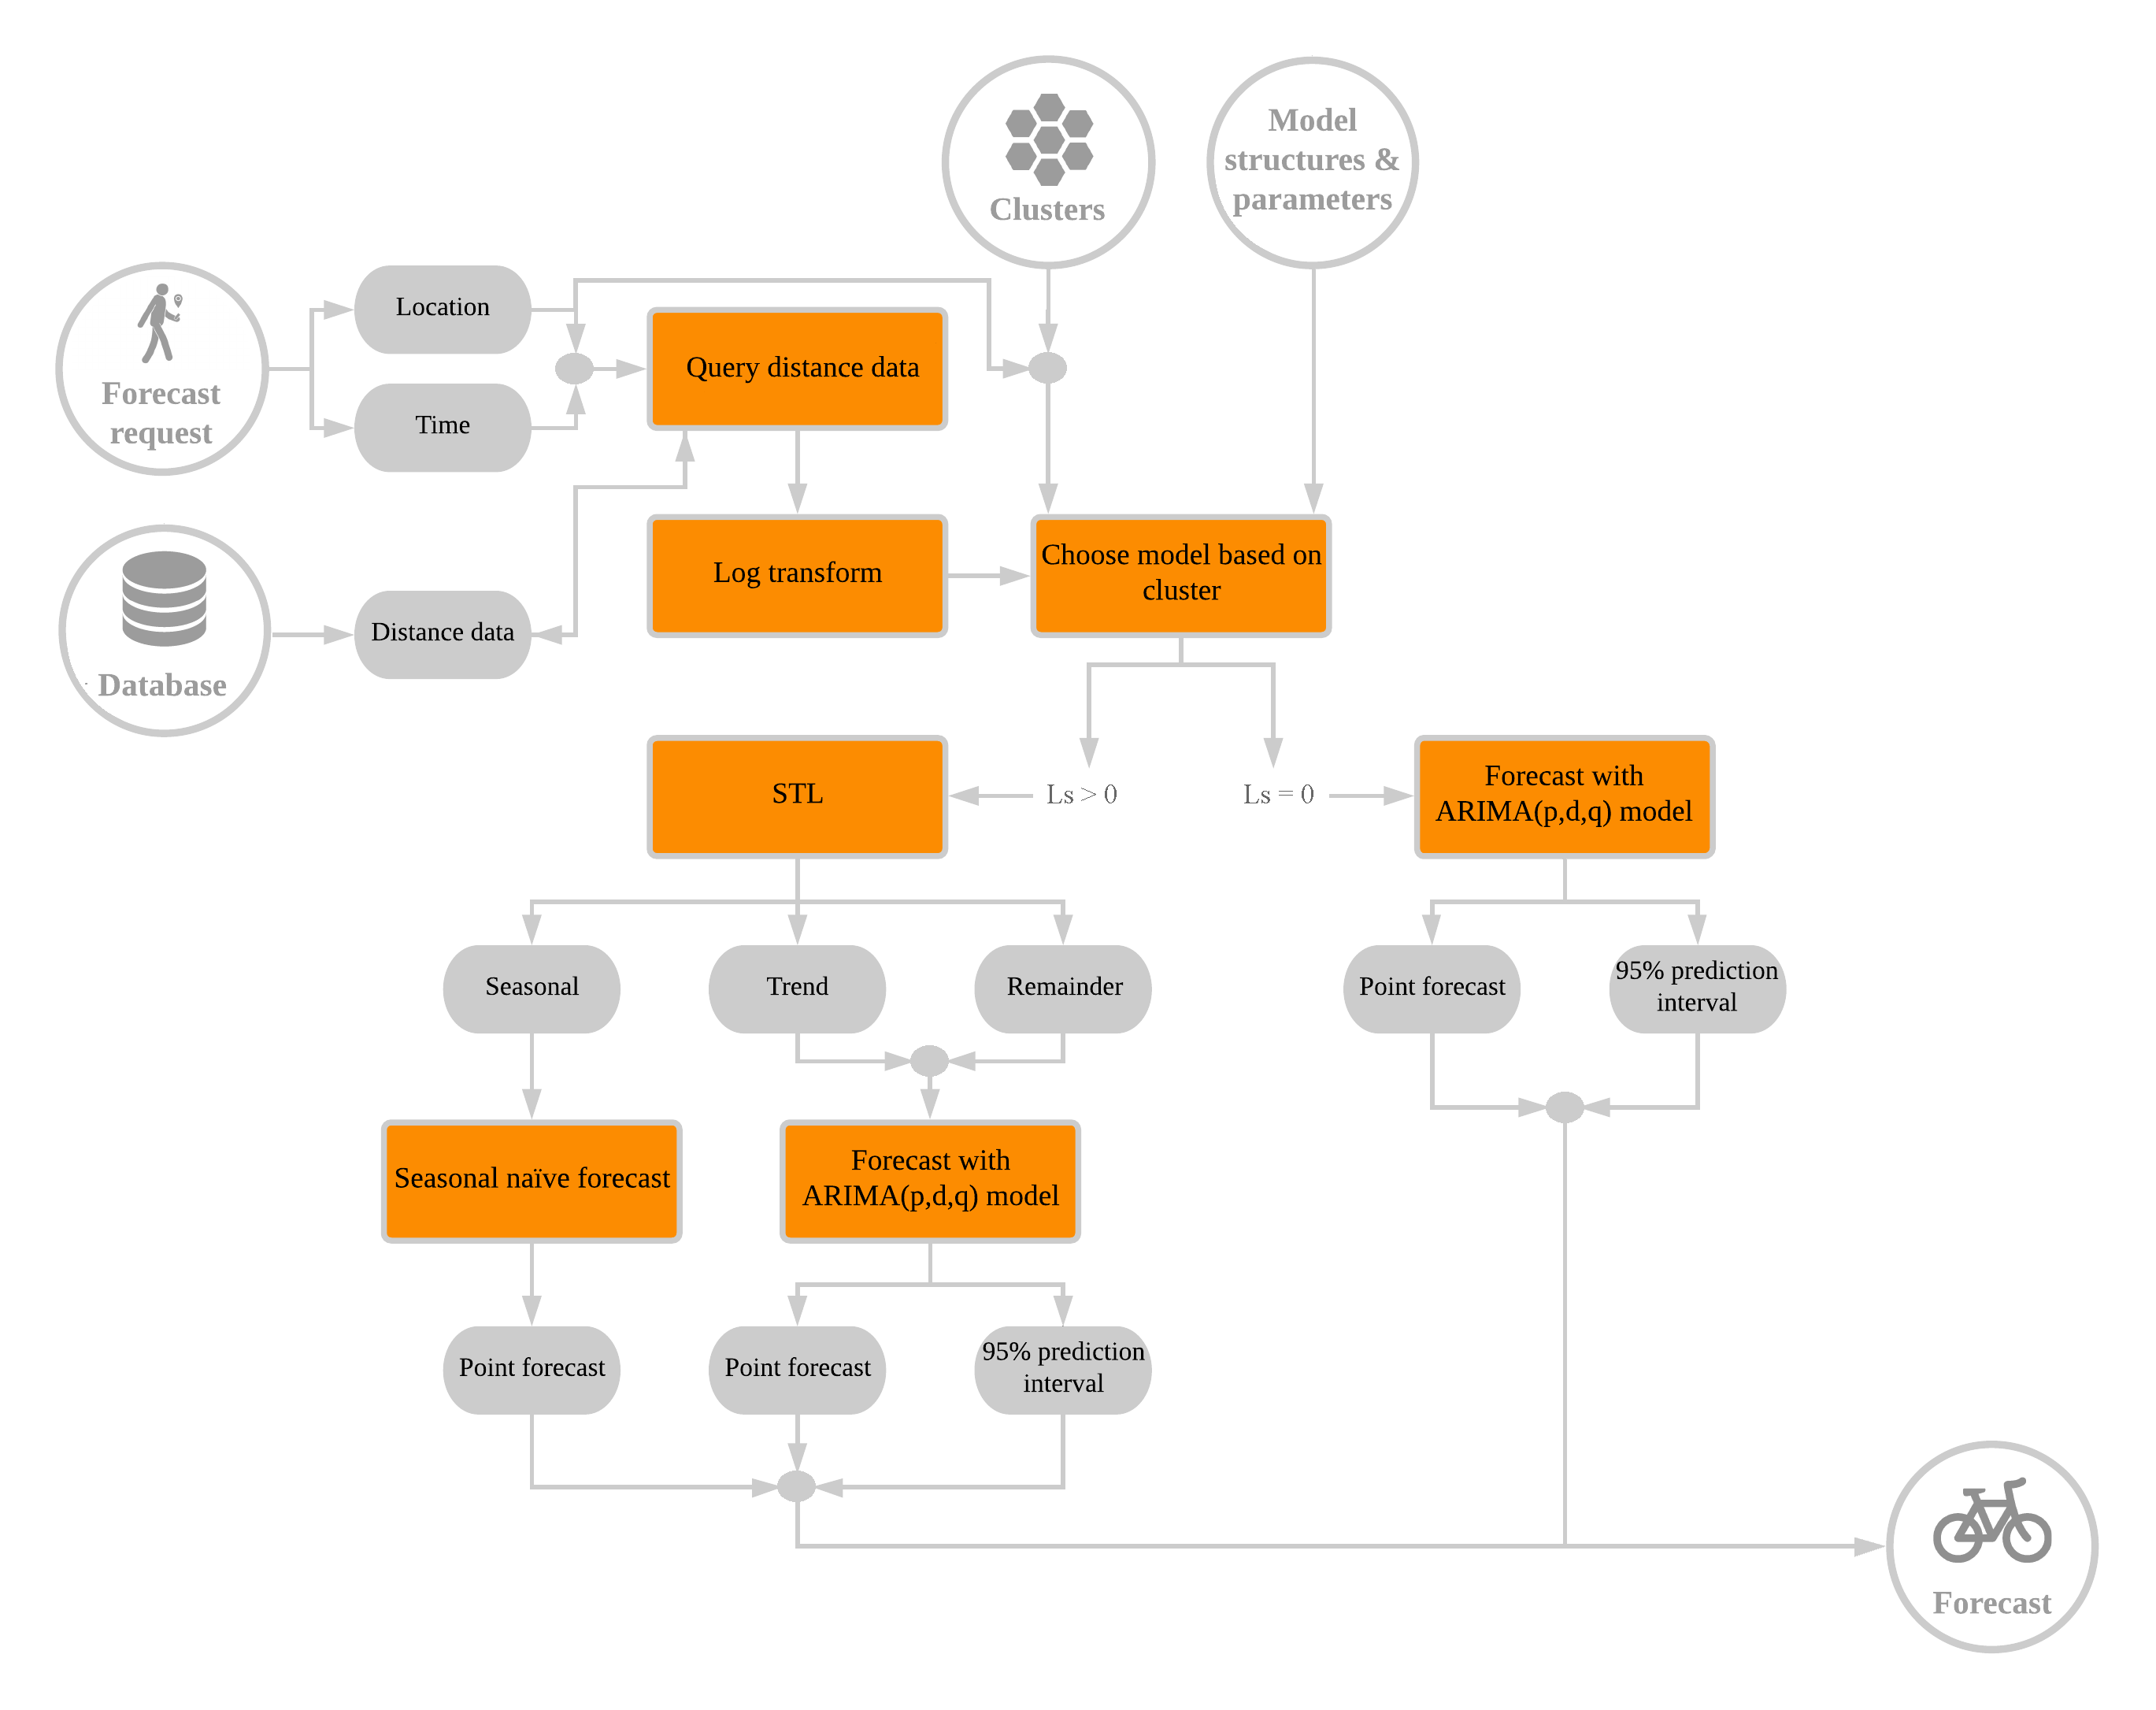
\includegraphics[width=\textwidth]{Figures/Forecastloop} \caption{Methodology of the forecast loop}\label{fig:forecastloop}
\end{figure}
\chapter{Data and experimental
design}\label{data-and-experimental-design}

This chapter describes the case study that was done to test the
performance of DBAFS. It is structured as follows. First, the
characteristics of the bike sharing system that served as a data source
for the experiment, are presented. The data retrieval process is
described in section two. Finally, the third section explains into
detail the methodology of the experiment itself.

\section{Data source}\label{data-source}

DBAFS' forecasting power was evaluated with data from the dockless PBSS
of San Francisco, California. The system there is exploited by JUMP
Bikes (\url{https://jump.com/}), an American company founded in 2010,
that went through a rapid development after being acquired by ride
hailing giant Uber in April 2018 (Khosrowshahi,
\protect\hyperlink{ref-uber2018}{2018}). In February 2019, JUMP was
active in 16 cities in the United States, as well as in Berlin, Germany.
All provided bicycles have electric pedal assistance, up to a maximum
speed of 32 km per hour.

In January 2018, the San Francisco Municipal Transportation Agency
(SFMTA) offered JUMP Bikes the city's first offical, exclusive permit to
operate a dockless PBSS, for an 18 month trial period, in order to
``evaluate, collect data, and assess whether further increases would
serve the public interest'' (Jose,
\protect\hyperlink{ref-sfmta2018one}{2018}\protect\hyperlink{ref-sfmta2018one}{a}).
SFMTA allowed up to 250 bikes in a system area of approximately 47
km\(^2\), which is shown in Figure 4.1. After nine months, a mid-point
evaluation lead to the allowance of expanding the fleet to 500 bikes
(Jose,
\protect\hyperlink{ref-sfmta2018two}{2018}\protect\hyperlink{ref-sfmta2018two}{b}).

The JUMP Bikes system in San Francisco, works as follows. A user needs
to download the JUMP mobile application and create an account. The app
shows the real-time locations of all available bikes. An available bike
can be unlocked with a unique code that is send to the user account. A
single trip costs \$2 for a total time of 30 minutes. For every minute
that exceeds the 30 minute timeframe, \$0.07 will be charged. Options
for subscription pricing, with a fixed amount per month or year, are not
available.

It is possible to reserve a bike up to 30 minutes before unlocking it.
In that case, the bike will not be labeled as available anymore, and can
not be taken by another user. However, the trip clock starts ticking
from the moment of reservation. When a user wants to stop somewhere
during a ride, the bike can be put `on-hold' for maximum an hour,
meaning that the bike stays inavailable during the stop. Also in this
case, the regular fee will be charged. When ending the ride, the bike
needs to be locked legally to a fixed object. Not doing so, will result
in a fee of \$25. Additionally, leaving the bike outside of the system
area, results in a \$25 fee as well (Harris,
\protect\hyperlink{ref-harris2018}{2018}).

Since all JUMP bikes are electric, battery life forms an important
issue. A fully charged bike can travel 48 to 64 kilometers with the
pedal assist. Bikes with a batterly level of less than 25\% are
collected, and charged. Furthermore, other bikes are regularly charged
during nightime. Charging takes in most cases about four to six hours,
and is done in a JUMP Bikes depot. Some of the charged bikes are placed
outside of the depot, where they can be picked up, while others are
redistributed over the system area. In the near future, this process
will change considerably, since the newly produced bikes, which will be
introduced in the first months of this year, have swappable batteries,
such that there is no need anymore to bring low-battery bikes to the
depot (Foley, \protect\hyperlink{ref-foley2018}{2018}).

In the first year of the trial period, 63000 users took over 625000
trips. On average, trips were 4.2 kilometers long, while around 1\% of
the trips, exceeded 24 kilometers. Each individual bike, was on average
used seven times per day. In september 2018, this was over eight times
per day. Even when the size of the fleet doubled in October 2018, the
utilization remained consistent until the first half of November, when
it started to decrease slightly, due to cold weather (Rzepecki,
\protect\hyperlink{ref-jump2019}{2019}). While the demand is high, the
supply is still restricted by SFTMA, putting extra emphasis on the need
for efficient rebalancing, and accurate bike availability forecasts.
\begin{figure}[h]
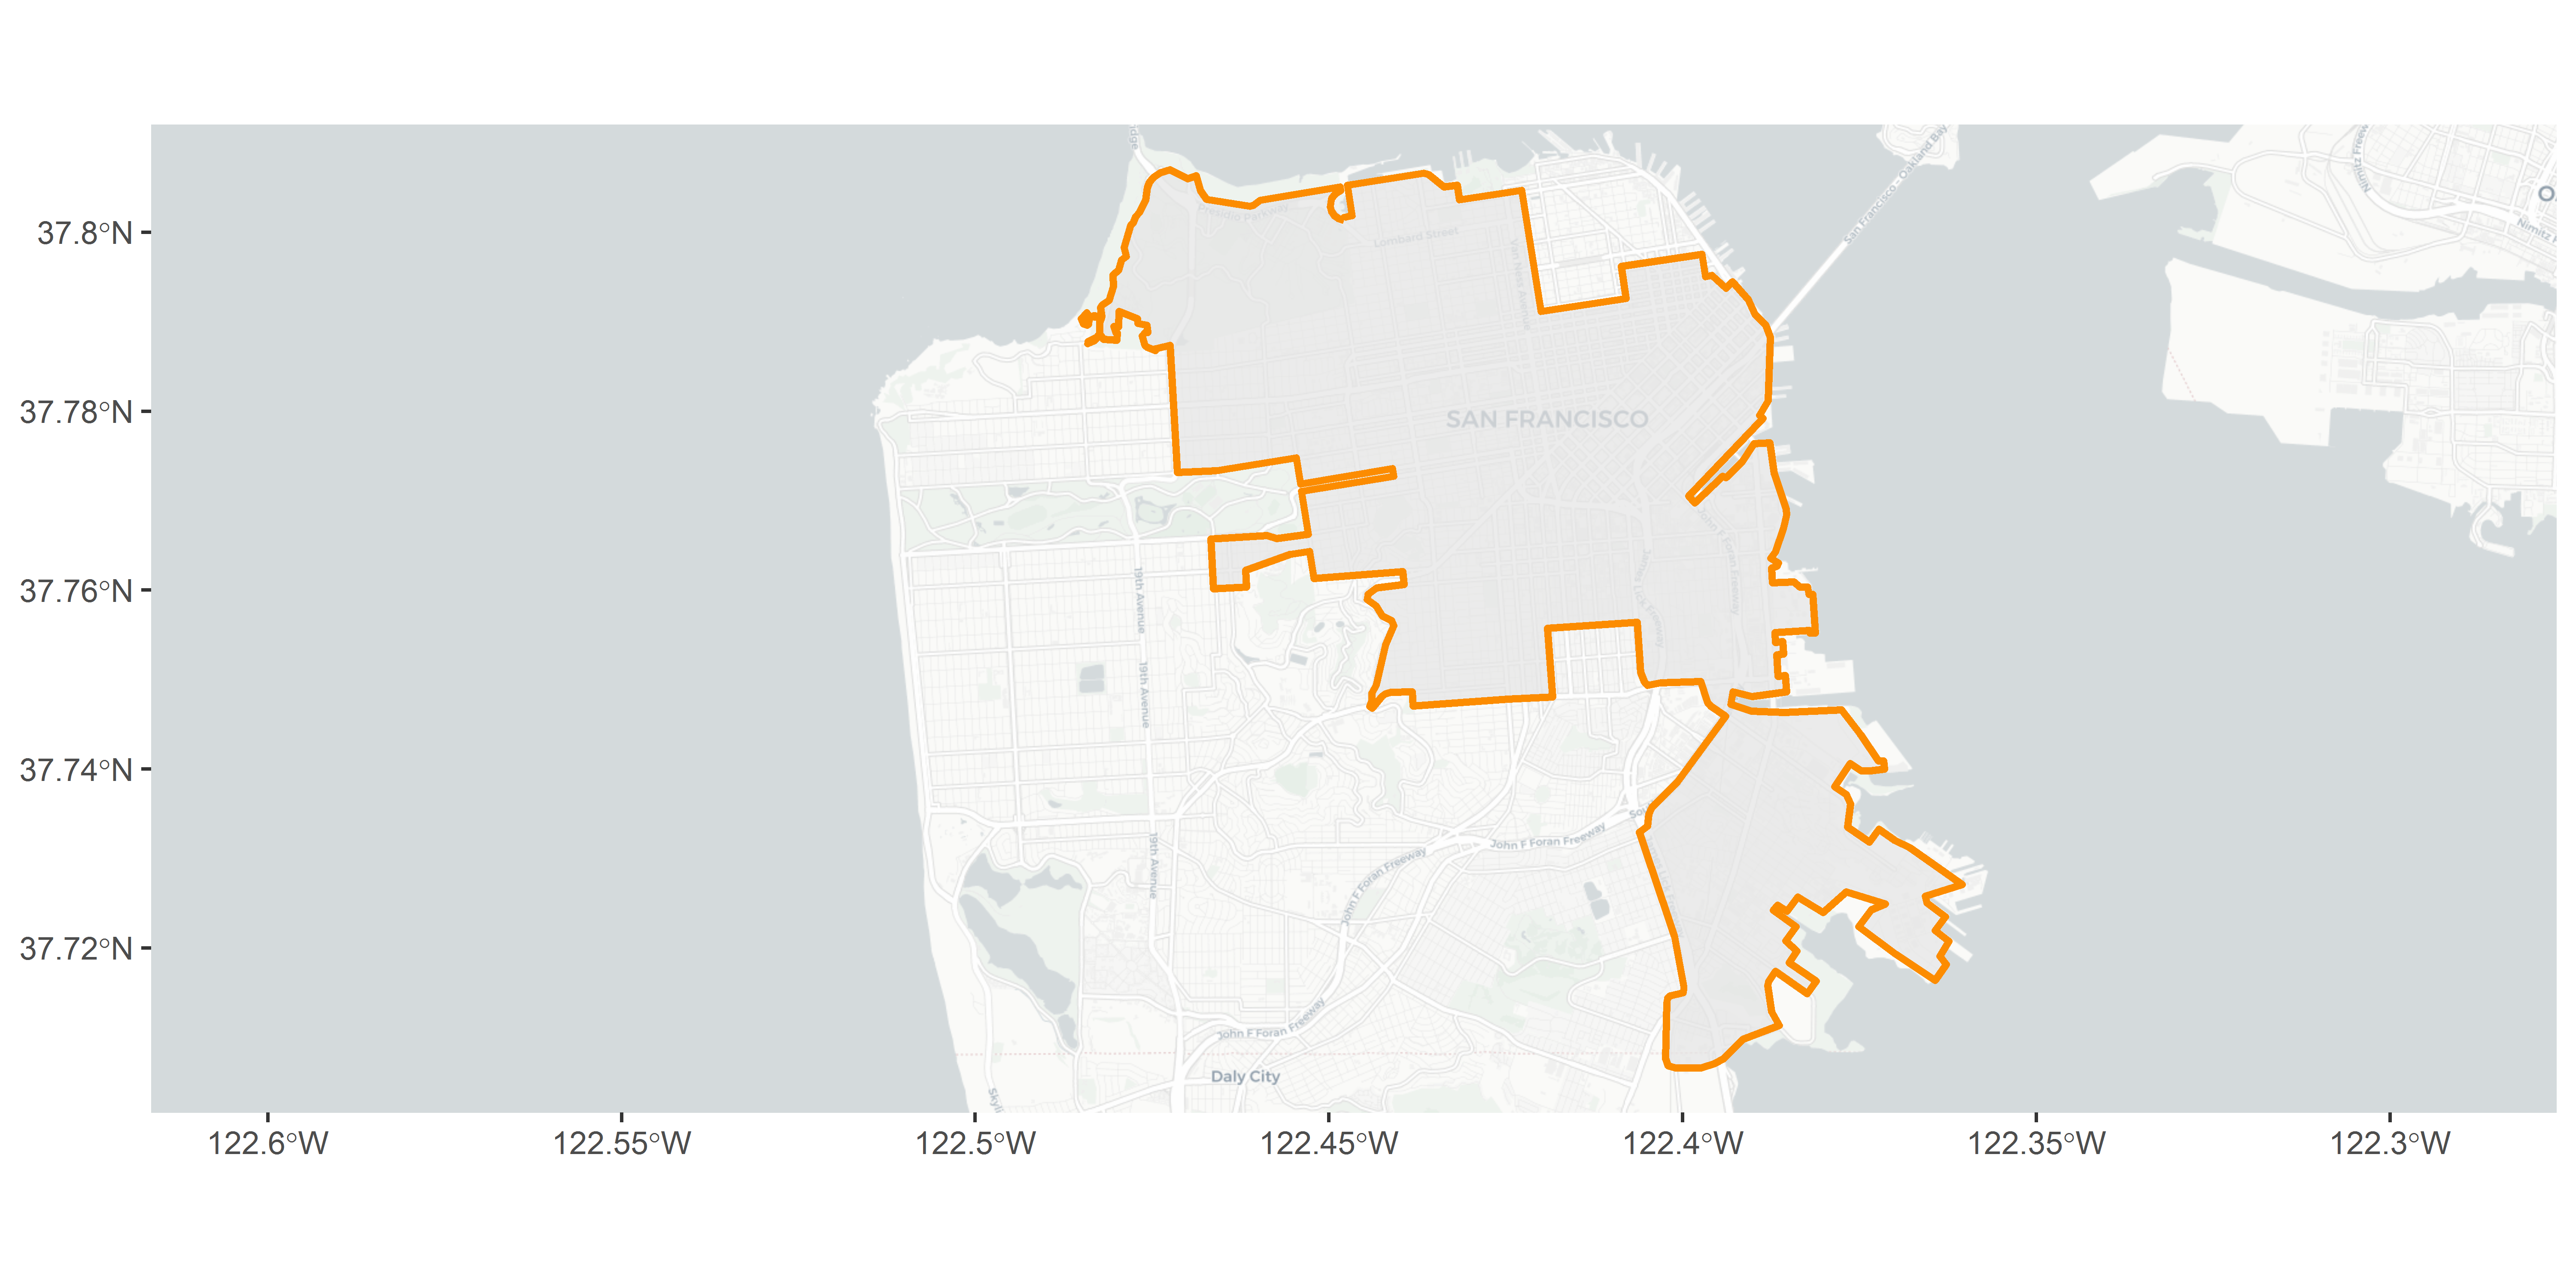
\includegraphics[width=\textwidth]{Figures/systemarea} \caption{System area of JUMP Bikes in San Francisco}\label{fig:systemarea}
\end{figure}
\section{Data retrieval}\label{data-retrieval}

JUMP Bikes provided access to a database containing the geographical
locations of their available bikes in San Francisco. The database
fulfilled all DBAFS requirements described in section 3.4. Data
collection started at September 9th, 2018, 15:41:08, Pacific Daylight
Saving Time (PDT). The data had a temporal resolution of one minute,
meaning that every minute, the location of each available bike in the
system was recorded. Timestamps were stored with six-digit precision.
Because of that, the time of recording was not exactly the same for each
available bike, but could vary up to a few seconds. Therefore, before
using the data in DBAFS, all timestamps were truncated to minute
precision.

\subsection{Distance data}\label{distance-data-1}

When calculating distances, only the historical data at every quarter of
an hour were used in the experiment. Hence, \(i_{s}\) was set equal to
fifteen minutes. There were several reasons for this choice. Firstly, it
is not expected that the data change drastically from minute to minute.
That is, using data with a temporal resolution of one minute will
probably not contain a lot more information than using data with a
temporal resolution of fifteen minutes. Consequently, if a forecast for
a specific timestamp is in practice a forecast for a few minutes
earlier, this will not be problematic. On the other hand, using only
data every fifteen minutes will decrease the size of the data with a
factor fifteen, and speed up computations considerably. Furthermore, a
lower order ARIMA(\(p\), \(d\), \(q\)) model can be used to capture the
same patterns in the data. This is important, since lower order models
will result in lower errors arising from parameter estimation (Brockwell
\& Davis, \protect\hyperlink{ref-brockwell2002}{2002}). After defining
\(i_{s}\), distance data pre-processing steps on the JUMP Bikes database
server were taken as described in section 3.4.1.

\subsection{Usage data}\label{usage-data-1}

Based on the specific knowledge of the JUMP Bikes system presented in
section 4.1, an extra restriction was added to the in section 3.4.2
described process of retrieving pick-ups from the original data. If a
feature that was initially considered to be a pick-up, was not followed
by a drop-off within a two hour timeframe, the feature was removed from
the usage data. Taking into account the average trip length of only 4.6
kilometers, the fact that trips become more expensive after half an
hour, the maximum allowed reservation time of 30 minutes, and the
maximum allowed `on-hold'-time of one hour, the threshold of two hours
was considered to be a safe border. In this way, pick-ups that occur
because the system operator is collecting bikes to be charged
(i.e.~pick-ups that do not reflect the usage intensity of the system),
were taken out.

Of course, there may have been some real trips that were longer than two
hours. However, given that during the first year of the trial period
only 1\% of the trips exceeded a distance of 24 kilometers, and the
electric pedal assitance allows a speed of more than 30 kilometers per
hours, this was assumed to be a negligible share of the total number of
trips.

\section{Experimental design}\label{experimental-design}

\subsection{Training and test periods}\label{training-and-test-periods}

As mentioned in section 4.1, usage of the JUMP Bikes system in San
Francisco remained rather constant in September, October, and the start
of November. An exploratory analysis on the distance data at several
locations in the system area enabled to draw similar conclusions, with a
sudden change in temporal patterns after mid-November. Recall that in
DBAFS, parameter \(n_{w}\), the number of weeks between two passes
through the model loop, should be chosen such that an `old' model is not
used anymore when the patterns in the historical data have changed
considerably. Therefore, to test the performance of DBAFS in an adequate
way, both the period used for model building, called the \emph{training
period}, and the period used for forecasting, called the \emph{test
period}, should preferably fall within a timeframe where no large
changes in the data patterns occur. However, they should not overlap
each other either, since the forecasting performance of a model can only
be truly evaluated when forecasts are made for data that the model has
not seen yet.

The training period, used to query data for both the cluster and model
loop, spanned the first four full weeks (i.e.~2688 observations) in the
data collection period, from Monday September 17th, 2018, 00:00:00 PDT,
up to and including Sunday 13th, 2018, 23:45:00 PDT, as shown in Figure
4.2. Hence, a situation was simulated in which the weeks of data used
for clustering \(m_{c}\), and the weeks of data used for model building,
\(m_{m}\) were both set to be four weeks. Taking into account the size
and shape of the system area, along with some exploratory research on
the demographic characteristics of San Francisco, \(K\), the set of
integers containing all values considered as the number of desired
clusters \(k\), was chosen to be \{\(3, 4, 5, ..., 10\)\}.

The obtained model structures and parameters resulting from the model
loop, were used to make several forecasts during a test period of one
week. For each forecast, two weeks of distance data were retrieved from
the database, such that in the case of a weekly seasonality, a
sufficient amount of data would be present for decomposition. Hence,
\(m_{f} = 2\). To make sure that in no case the data used for
forecasting would overlap with the data used for model building, a two
week period seperated the training and test period. That is, the test
week ranged from Monday October 29th, 00:00:00 PDT, up to and including
Sunday November 4th, 2018, 23:45:00 Pacific Standard Time (PST), as
shown in Figure 4.2.

Defining where and when to forecasts, was done by simulating real-world
forecast requests, and sending them to the forecast loop. To do this in
a realistic way, the following requirements had to be fulfilled.
\begin{itemize}
\tightlist
\item
  More forecast requests should occur at locations where the usage
  intensity of the system is higher.
\item
  More forecast requests should occur at times when the usage intensity
  of the system is higher.
\item
  It should be accounted for, that the times when the usage intensity is
  higher, can vary per location, and vice versa.
\end{itemize}
Bearing these requirements in mind, the following approach was
developed. All pick-ups during the test week were retrieved from the
database. Ten pick-ups per cluster where randomly sampled, guaranteeing
that each cluster was represented in the sample. Subsequently,
\(500-10 \times k\) pick-ups were randomly sampled from the remaining
ones, regardless to which cluster they belonged. This lead to a dataset
of 500 pick-ups in total, from which the location-timestamp combinations
were retrieved. Pick-ups reflect the usage of the bike sharing system.
That is, a random sample of them will contain more locations in areas
where the usage intensity is high, and more timestamps at times when the
usage intensity is high. Furthermore, the location and timestamp come as
a combination, rather than as separate entities. In this way, the
approach fulfills all three requirements mentioned above. The
location-timestamp combinations in the sample will from now on be
referred to as the \emph{test points}.

Starting from the timestamp of the test point, all time lags up to one
day ahead, i.e.~96 time lags in total, were forecasted. Having 500 test
points, in total, 48000 forecasts were made. To evaluate their
performance, historical distance data for all forecasted time lags were
retrieved from the database, and the forecast RMSE (see section 2.4.2.6)
was calculated for each test point seperately.

By using the approach described above, the reported overall forecast
errors will be dominated by those made during peak hours, when obtaining
accurate forecasts is generally harder, and in crowded areas, where
obtaining accurate forecasts is generally harder. However, this is
intended, because reporting a large amount of forecast errors made
during off-peak hours, and in non-crowded areas, or, alternatively,
using adjusted error metrics such as the RMSLE, may give results that
look nicer, but do not reflect the real usefulness of the forecasting
system.

To examine the forecasting power of DBAFS in a relative manner, all test
points were also forecasted 96 time lags ahead with a simple baseline
method. The naïve method, as described in section 2.4.3, was chosen for
this task. Therefore, the baseline forecasting system will from now on
be referred to as the Naïve Forecasting System (NFS). For each test
point, the RMSE's of the forecasts of NFS were calculated, and compared
to those of DBAFS.
\begin{figure}[h]
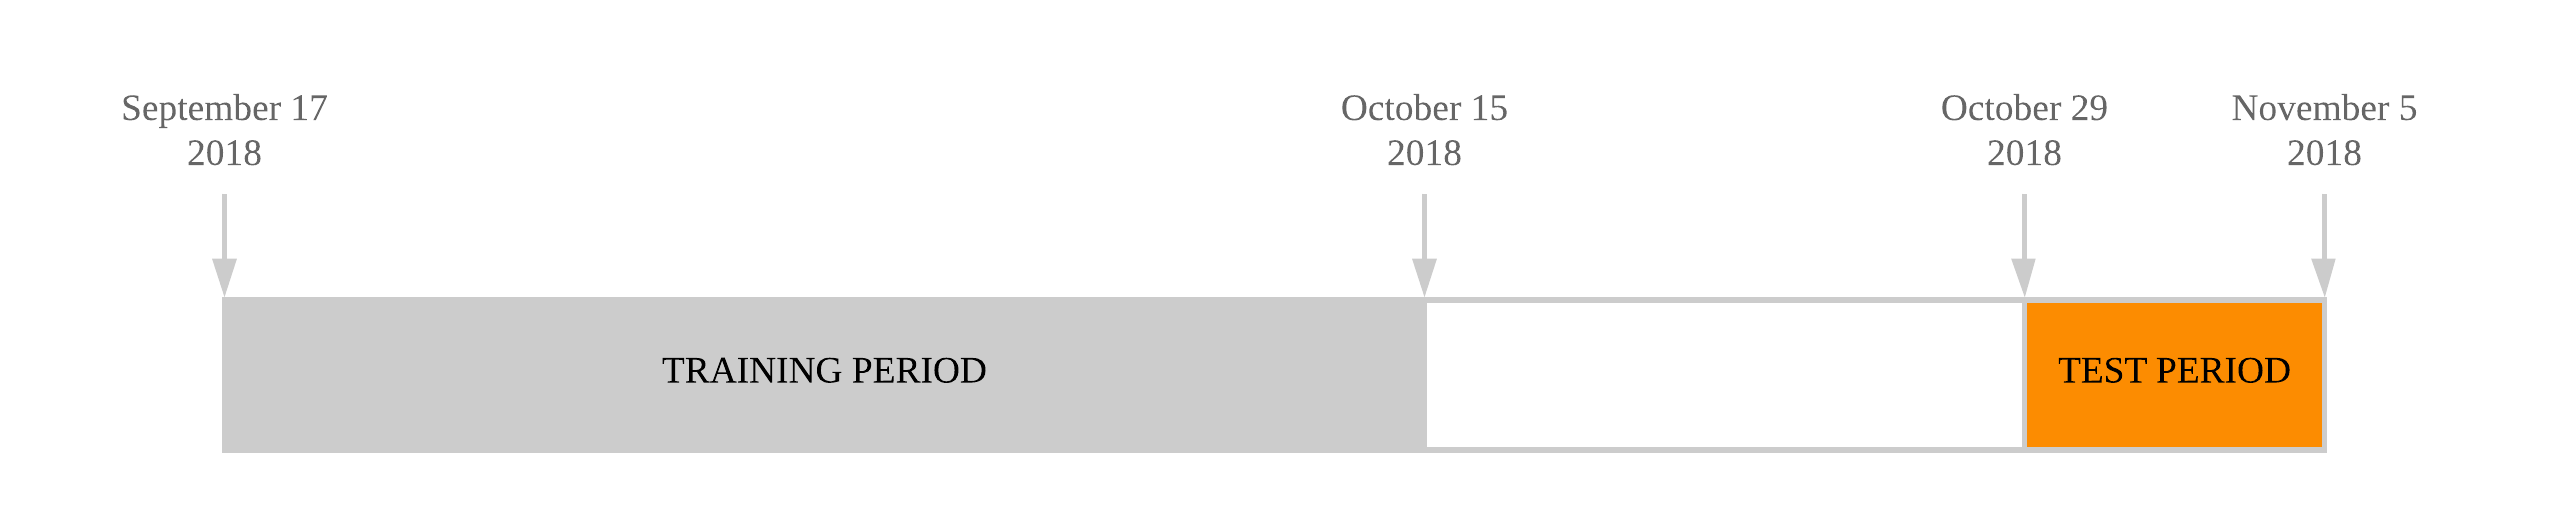
\includegraphics[width=\textwidth]{Figures/traintest} \caption{Training and test period}\label{fig:traintest}
\end{figure}
\subsection{Additional software}\label{additional-software}

On top of those mentioned in section 3.2, some additional R packages
were used for reporting the results of the experiment, as listed below.
\begin{itemize}
\tightlist
\item
  The \texttt{tsibblestats} package (Hyndman, O'Hara-Wild, \& Wang,
  \protect\hyperlink{ref-tsibblestats}{2018}) was used to estimate the
  ACF (see section 2.2.1) of time series.
\item
  The \texttt{tsfeatures} package (Hyndman, Kang, Talagala, Wang, \&
  Yang, \protect\hyperlink{ref-tsfeatures}{2019}) was used to calculate
  the spectral entropy (see section 2.2.3) of time series.
\item
  Data and results were visualized graphically with the \texttt{ggplot2}
  package (Wickham, \protect\hyperlink{ref-ggplot}{2016}). Additionally,
  the packages \texttt{tidyr} (Wickham \& Henry,
  \protect\hyperlink{ref-tidyr}{2018}), \texttt{dplyr} (Wickham,
  François, Henry, \& Müller, \protect\hyperlink{ref-dplyr}{2019}) and
  \texttt{tibble} (Müller \& Wickham,
  \protect\hyperlink{ref-tibble}{2019}) were used to transform some data
  into formats that are compatible with \texttt{ggplot2}.
\item
  Maps were created with the \texttt{ggspatial} package (Dunnington,
  \protect\hyperlink{ref-ggspatial}{2018}). Besides, with the
  \texttt{rosm} package (Dunnington,
  \protect\hyperlink{ref-rosm}{2017}), all basemap tiles were retrieved
  from CARTO (CARTO, \protect\hyperlink{ref-carto}{2018}).
\item
  For maps with a continuous color scheme, the \texttt{orange\_material}
  color scheme from the \texttt{ggsci} package (Xiao,
  \protect\hyperlink{ref-ggsci}{2018}) was used.
\end{itemize}
For the R code used in the experiment, see Appendix A.

\chapter{Results and discussion}\label{results-and-discussion}

This chapter presents and discusses the results of the experiment
described in Chapter 4. It is structured as follows. The first section
shows the clusters that resulted from the cluster loop, along with their
main characteristics, and the chosen locations of the model points.
Section two presents the structure of the models that were build in the
model loop, and the residual diagnostics for each them. Then, the third
section focuses on the accuracies of the forecasts, and their patterns
in both space and time. Finally, in the fourth section, the limitations
of DBAFS are discussed, and recommendations for possible improvements
are given.

\section{Clustering}\label{clustering}

Figure 5.1a shows the grid overlaying the JUMP Bikes system area in San
Francisco, including the centroid of each grid cell. In total, the grid
contains 249 cells, each 500 meter high and 500 meter wide.

Figure 5.1b shows the calculated number of pick-ups per grid cell,
during the training period. On average, there were 218 pick-ups per grid
cell, wich corresponds to approximately eight pick-ups per day. The
maximum number of pick-ups in a grid cell was 1985 (i.e.~71 per day on
average), while in 25 of the 249 grid cells, there were no pick-ups at
all. It can be seen that high counts of pick-ups occured in the grid
cells along the diagonal axis from south-west to north-east. Mainly in
the south-eastern corner of the system area, the usage intensity was
very low.

Figure 5.2 shows the temporal patterns of the usage data, with the
pick-ups per day of the week, and per hour of the day. Friday was the
day with on average the most pick-ups, while Saturday and Sunday had the
least. The busiest hours of the day, where 8:00 and 9:00, during morning
rush hours, and 16:00 and 17:00, during afternoon rush hours. The lowest
numbers of hourly pick-ups, as expected, occured during the night.
\begin{figure}[H]
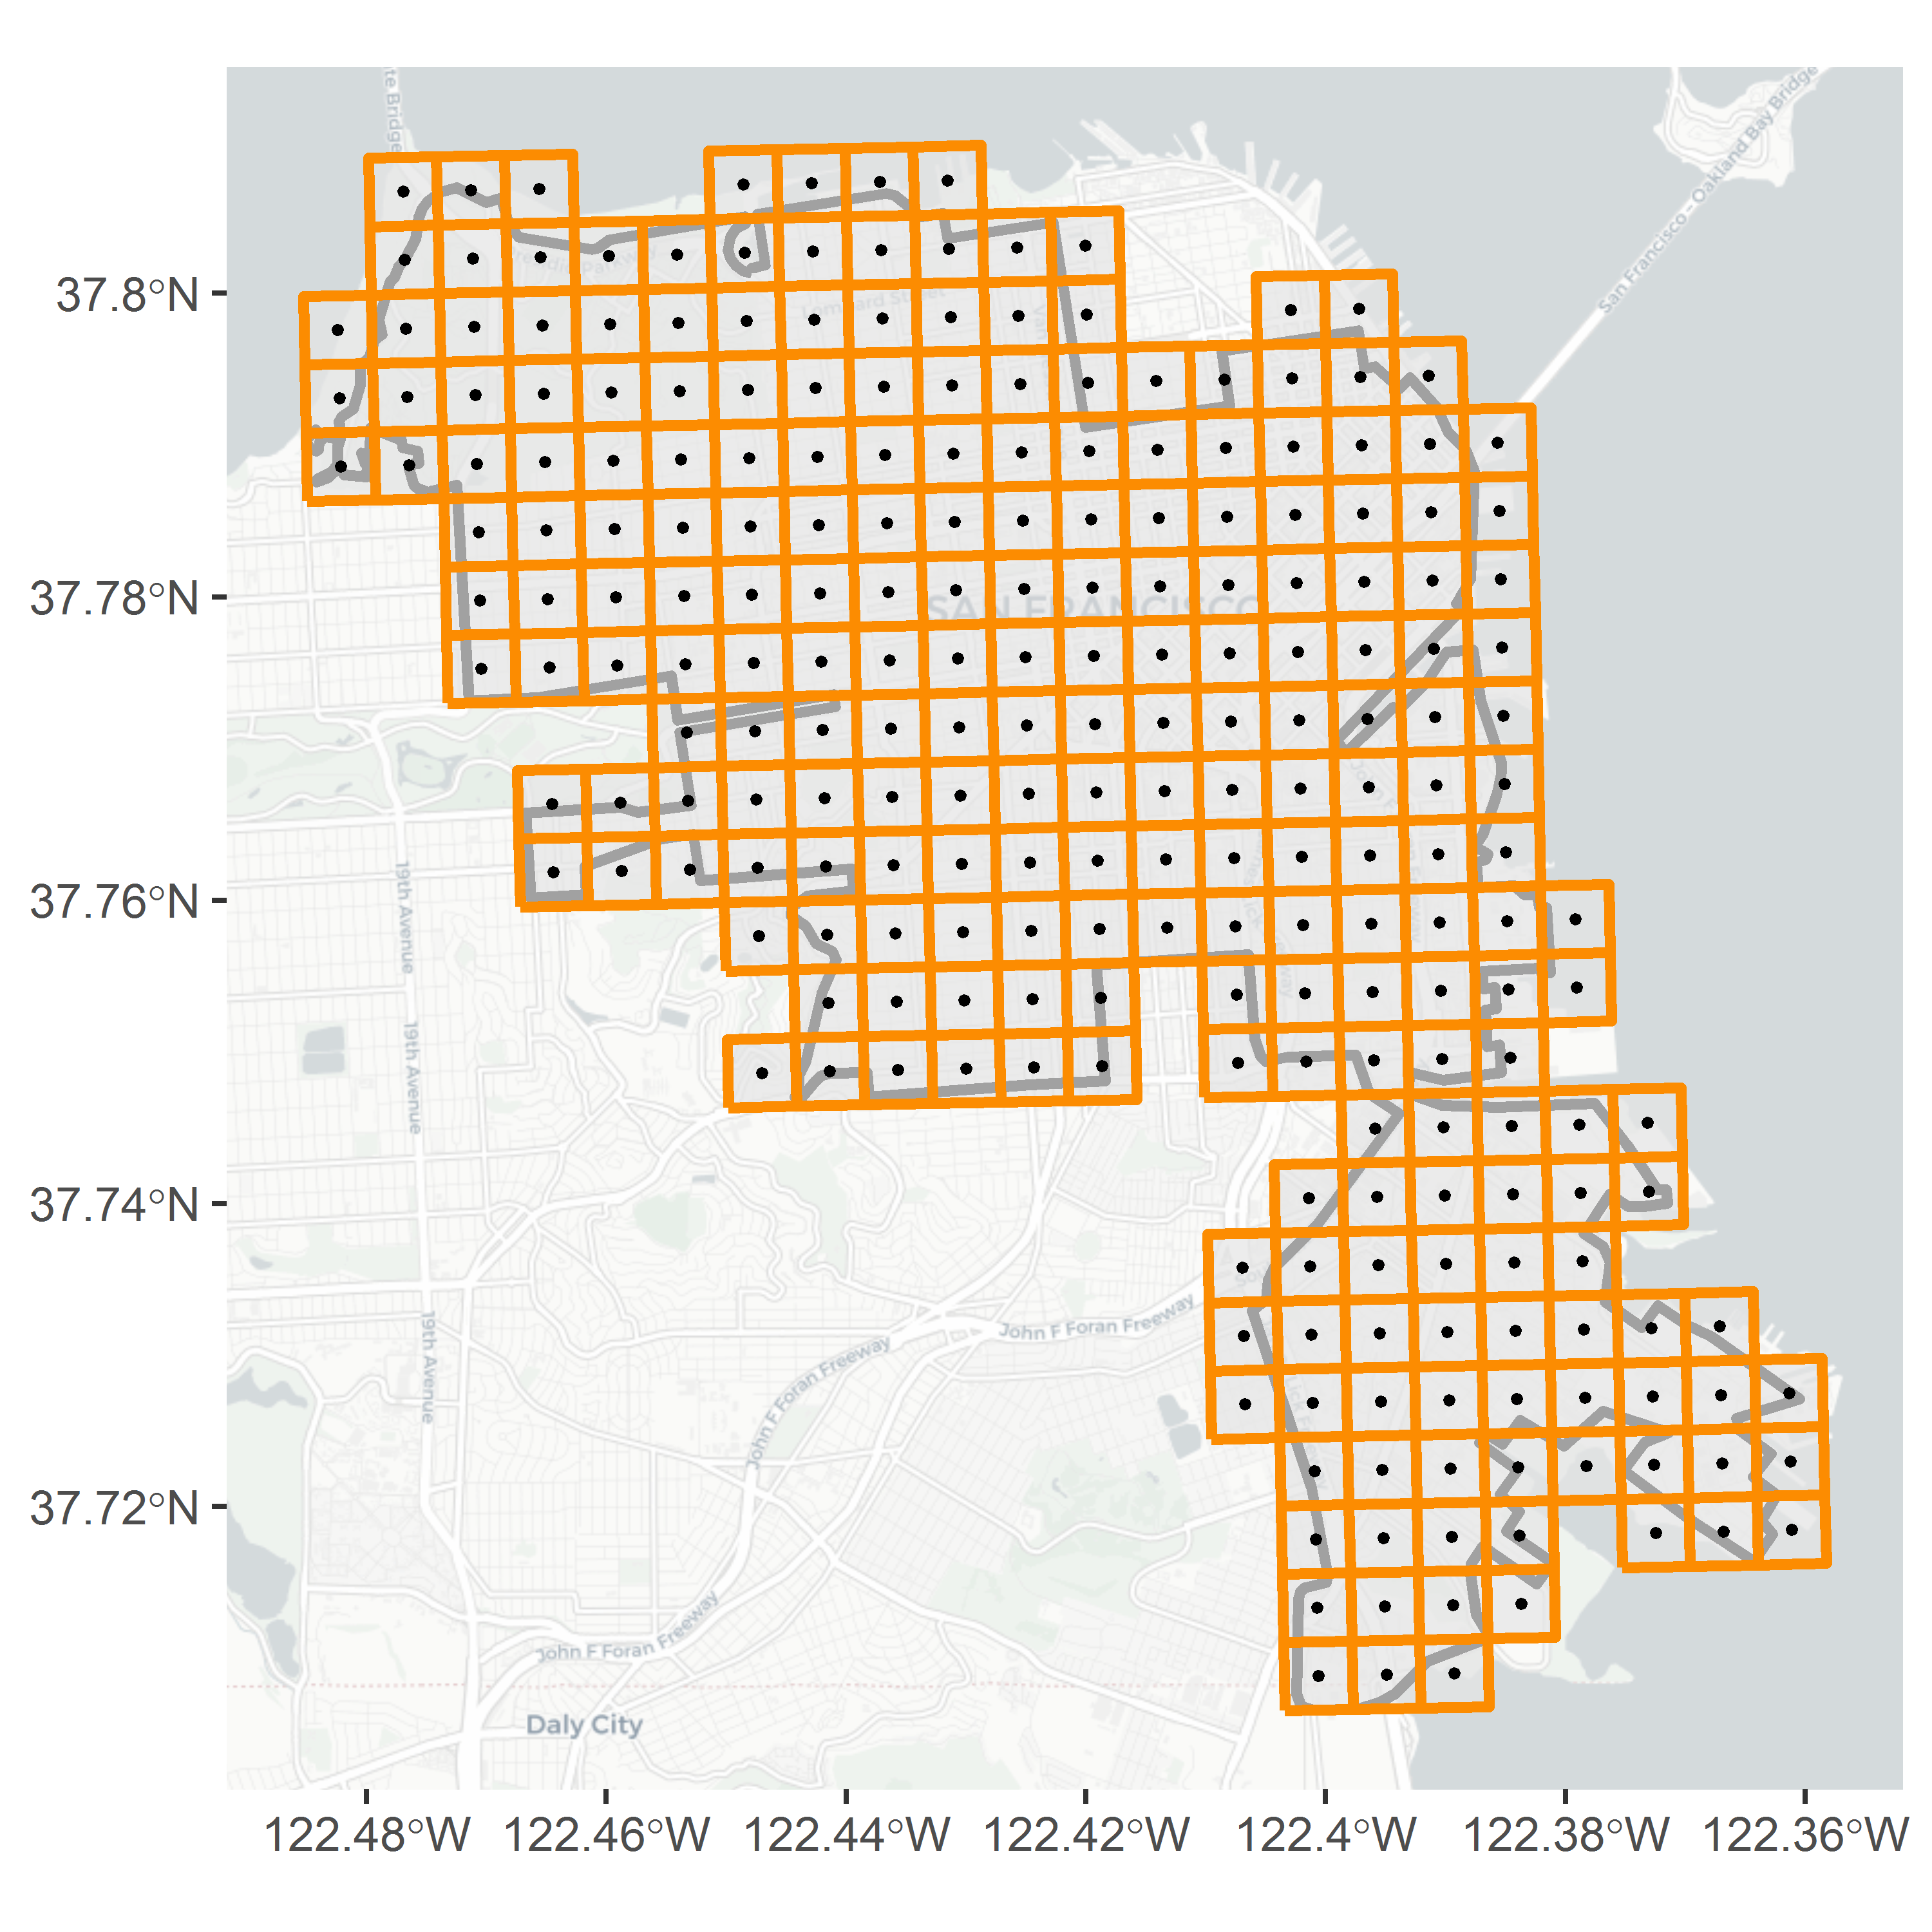
\includegraphics[width=0.5\linewidth]{Figures/grid} 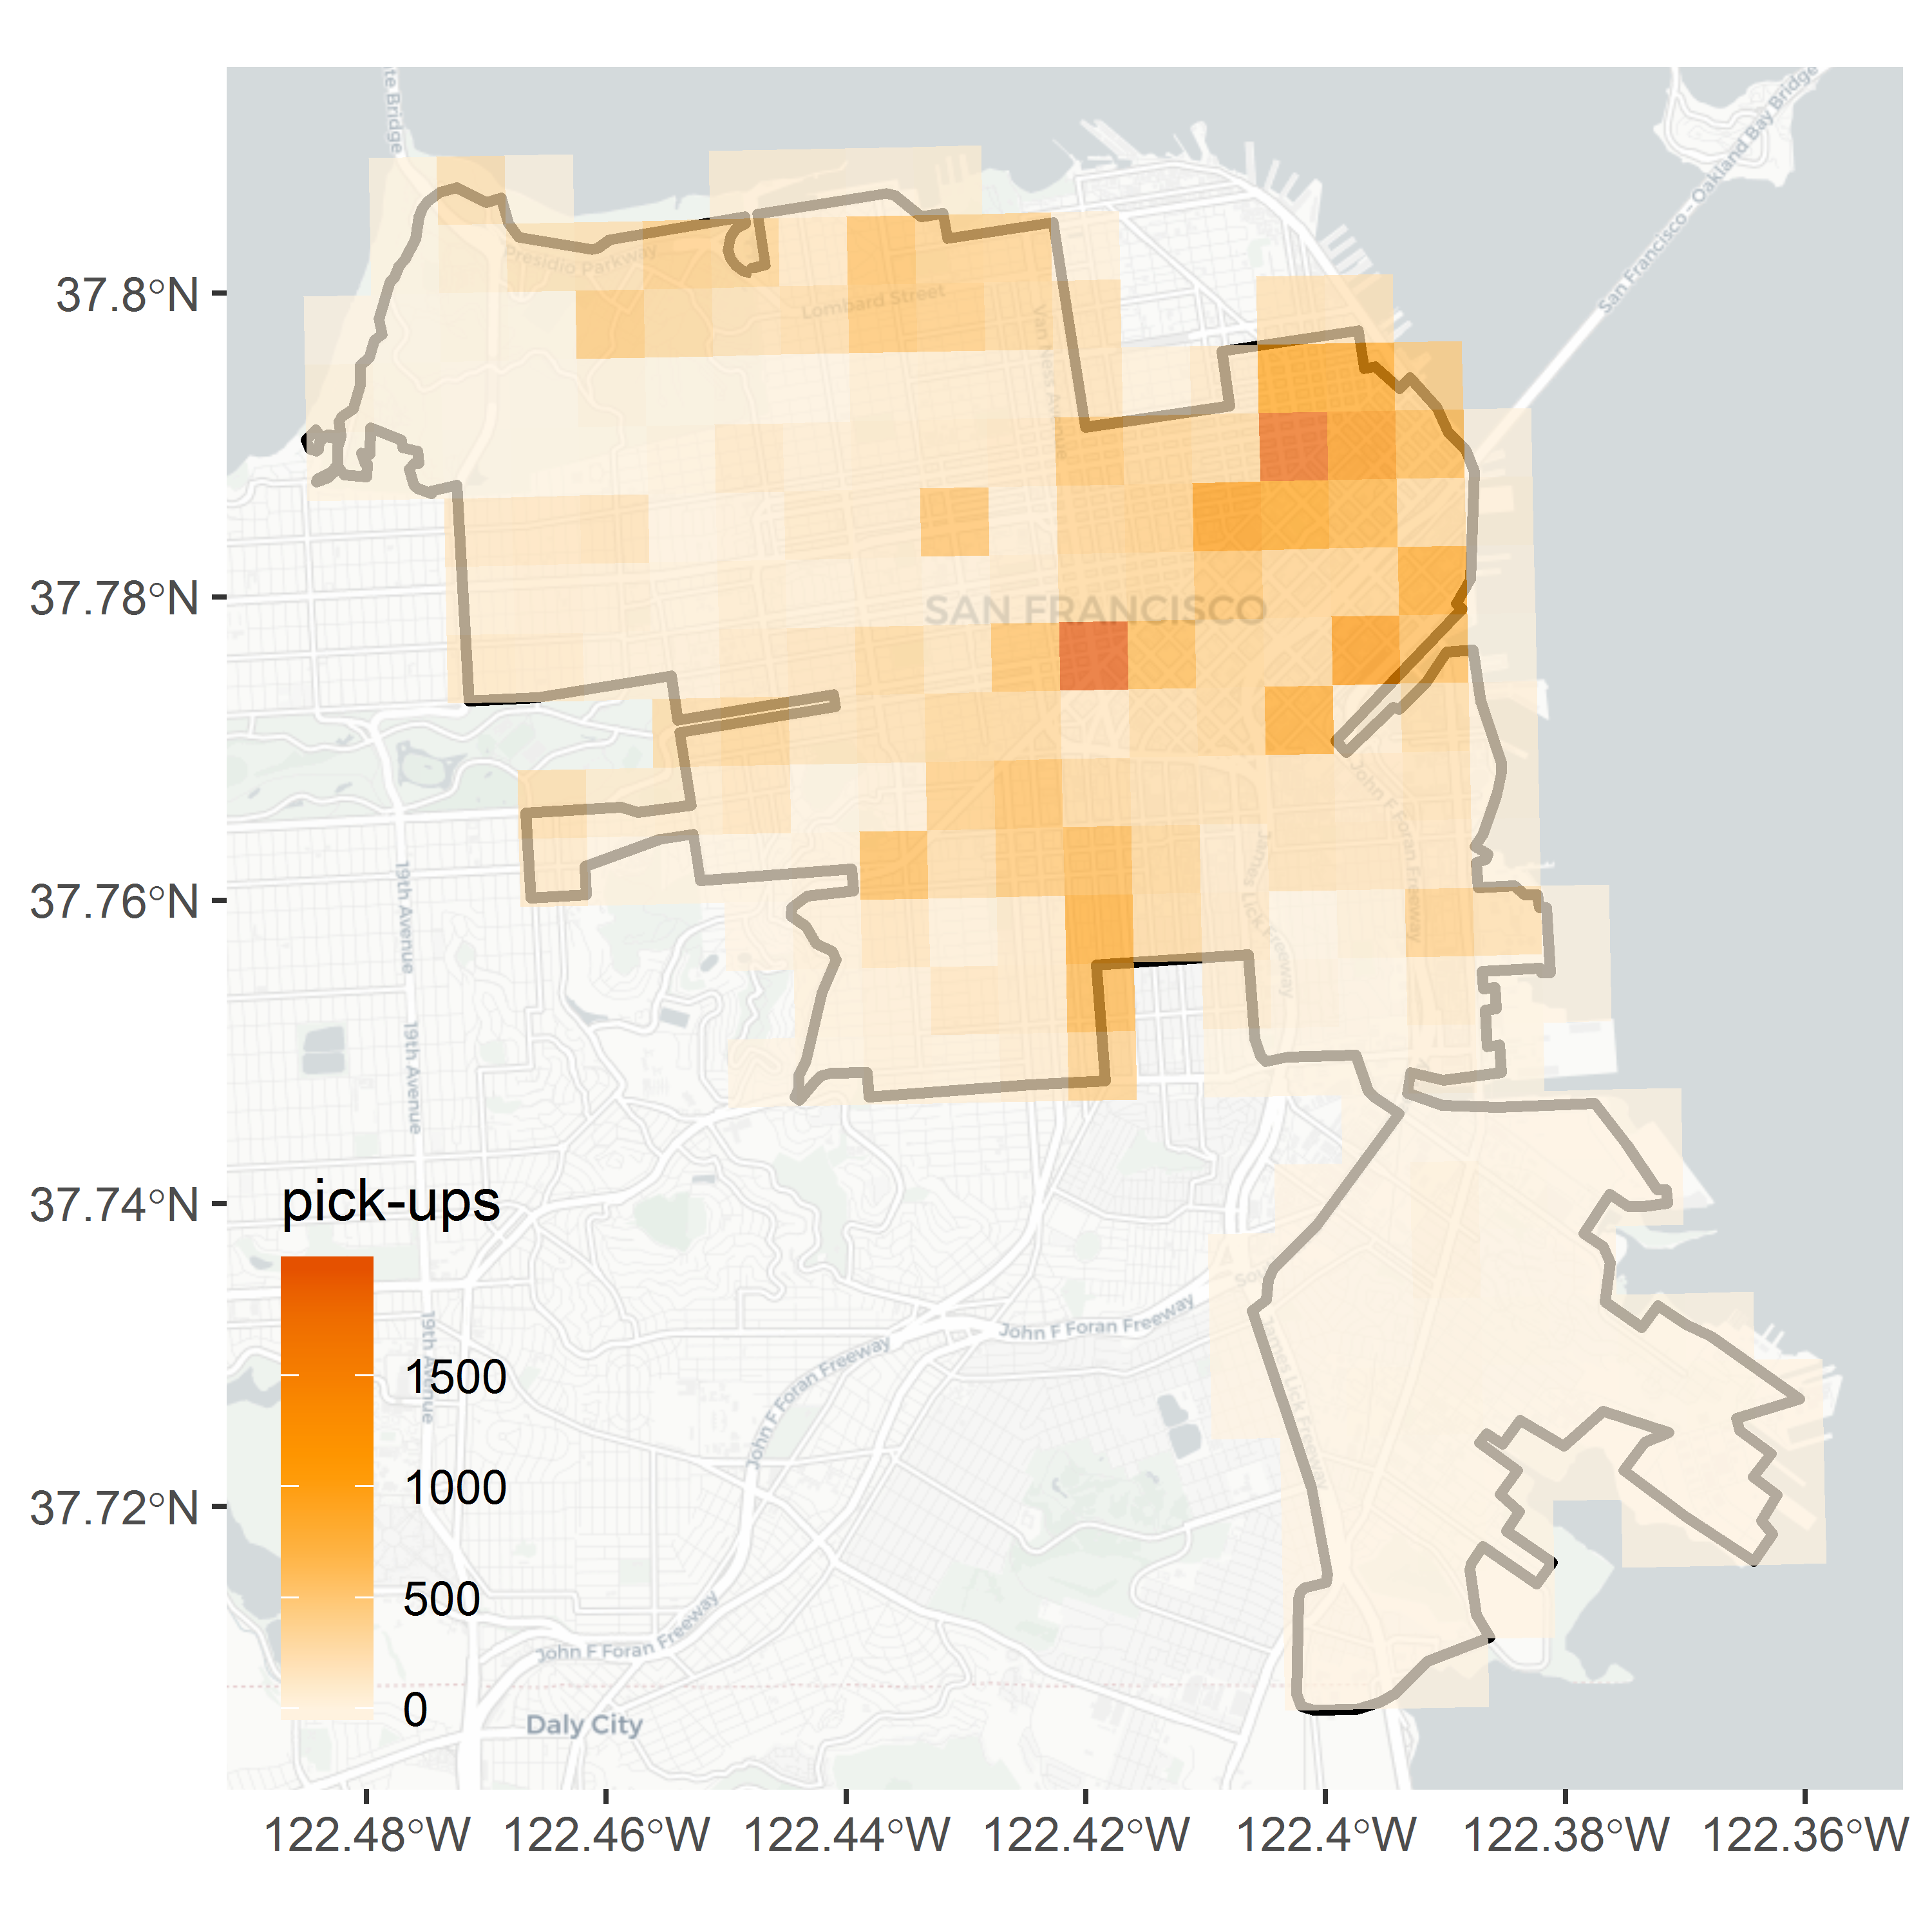
\includegraphics[width=0.5\linewidth]{Figures/pickups} \caption{a) grid overlaying the system area; b) number of pick-ups per grid cell}\label{fig:mapandgrid}
\end{figure}\begin{figure}[H]
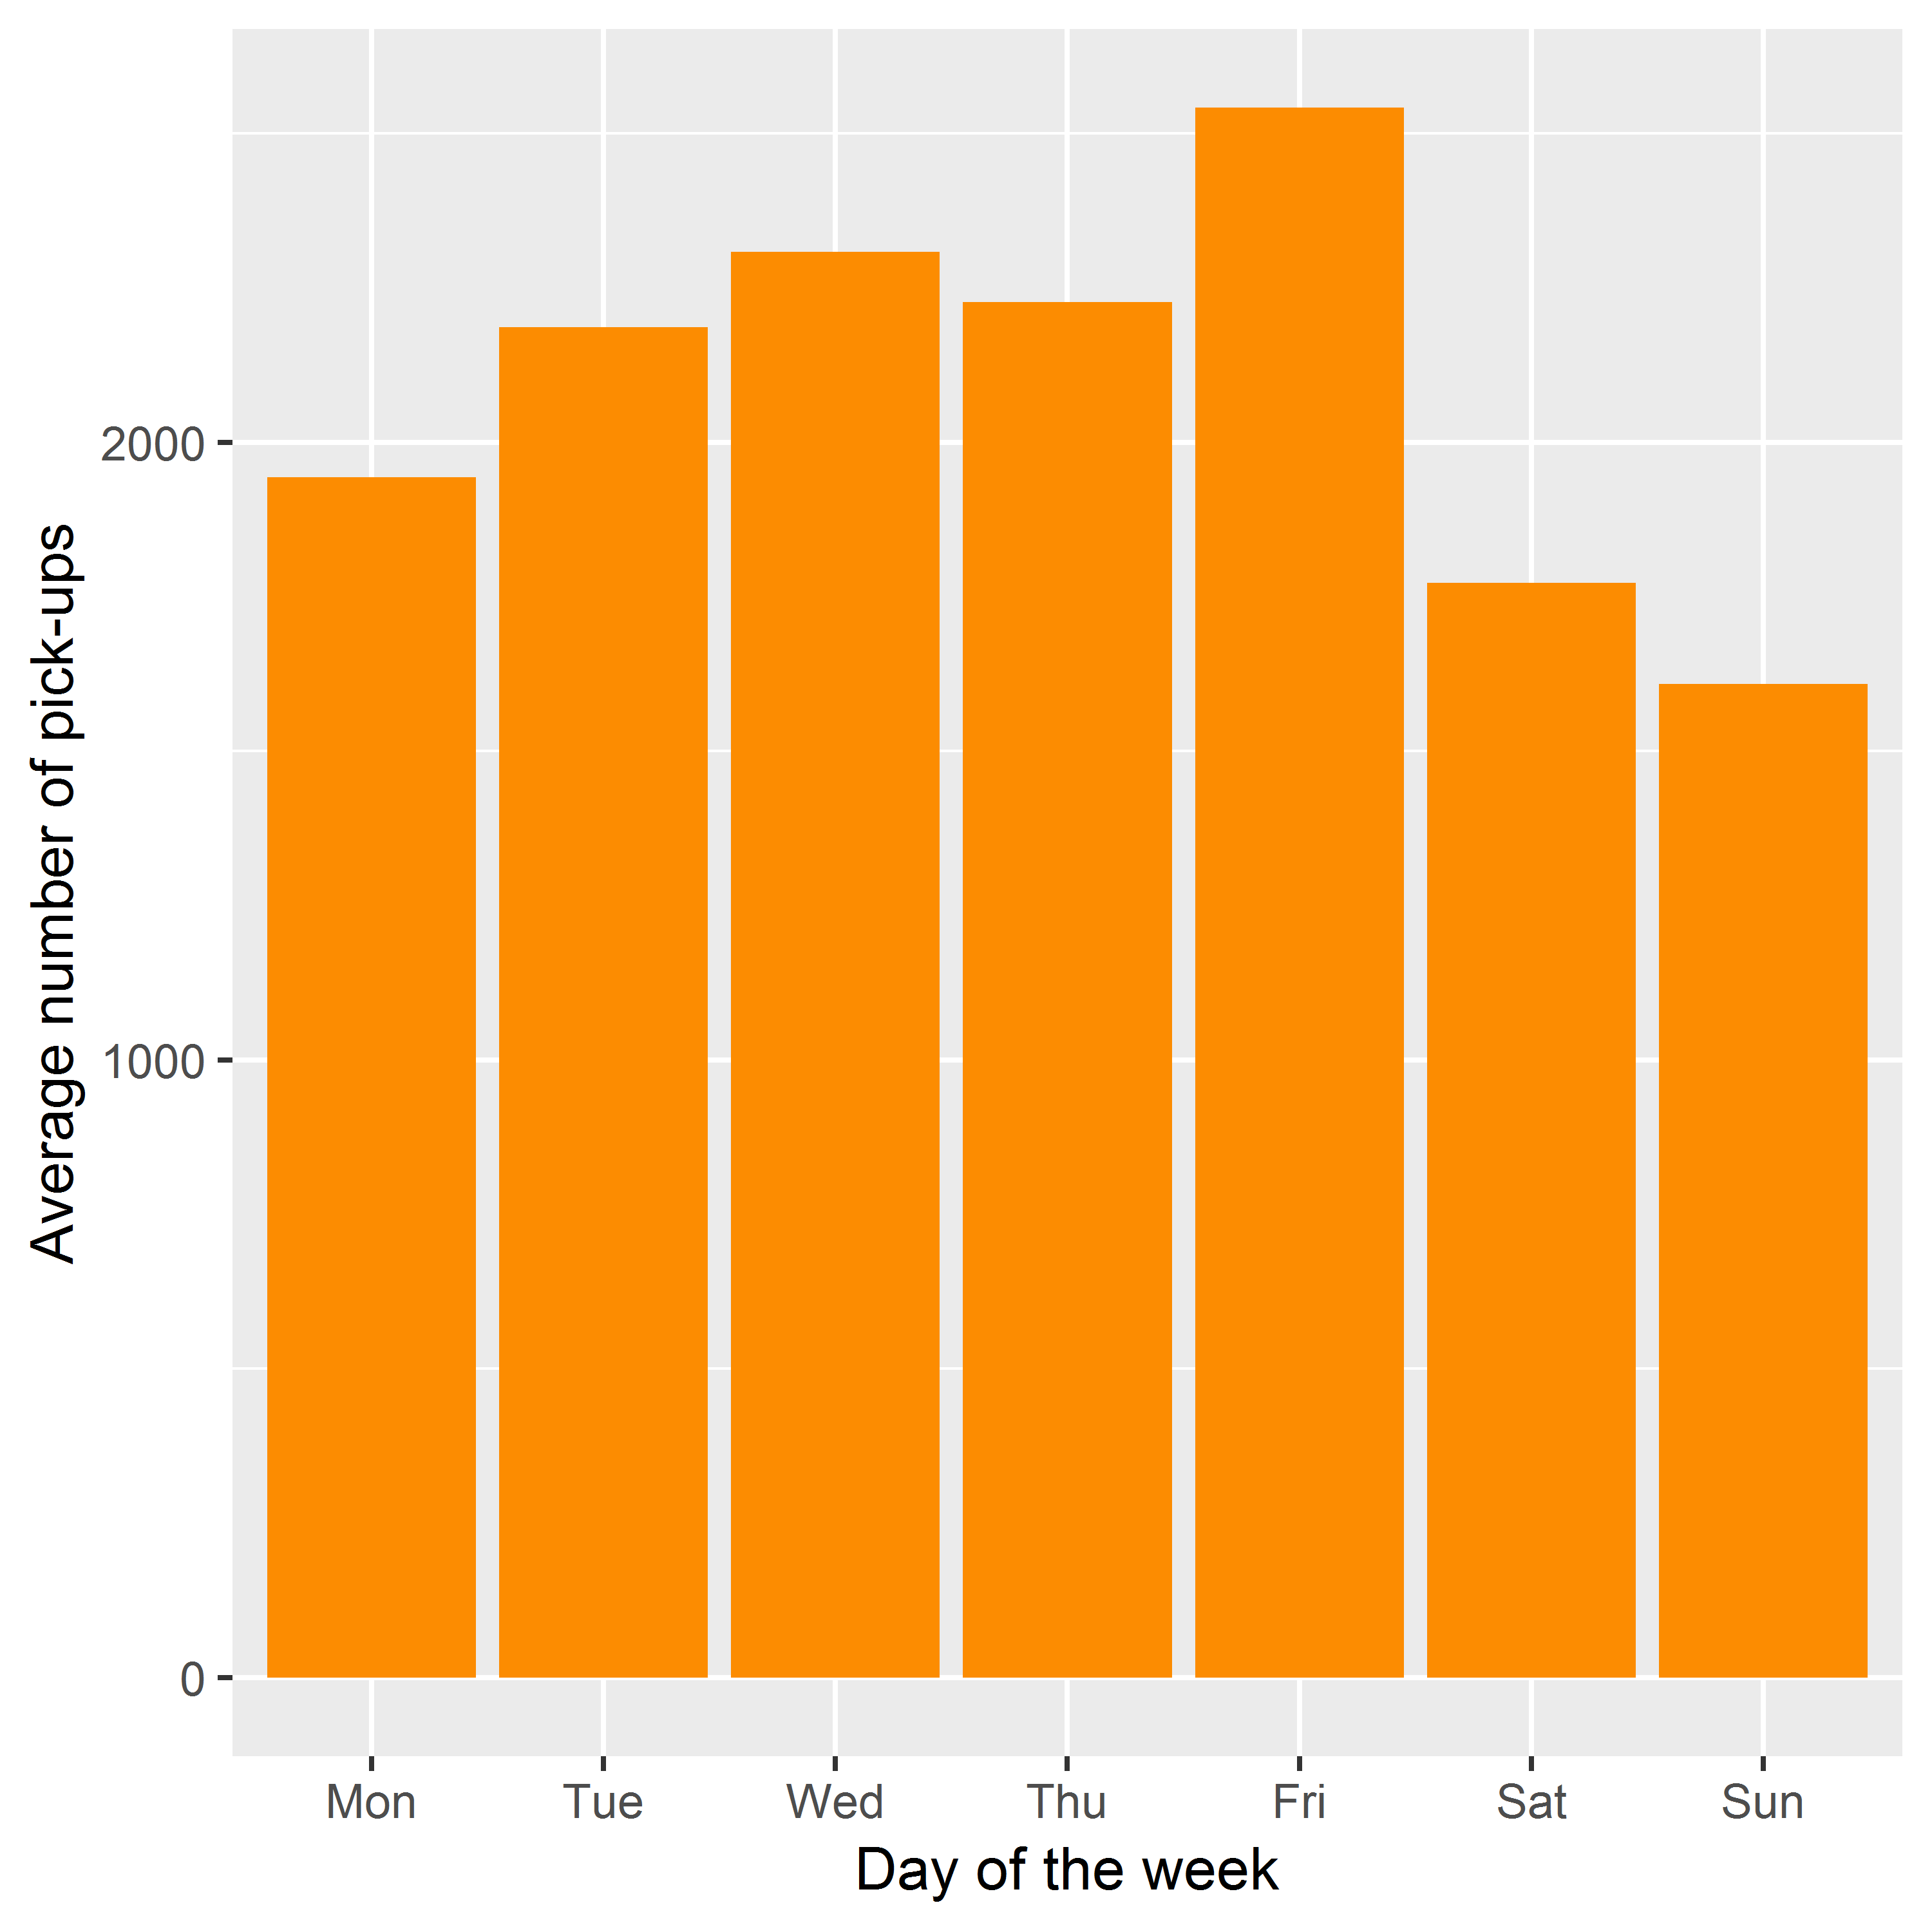
\includegraphics[width=0.5\linewidth]{Figures/usageday} 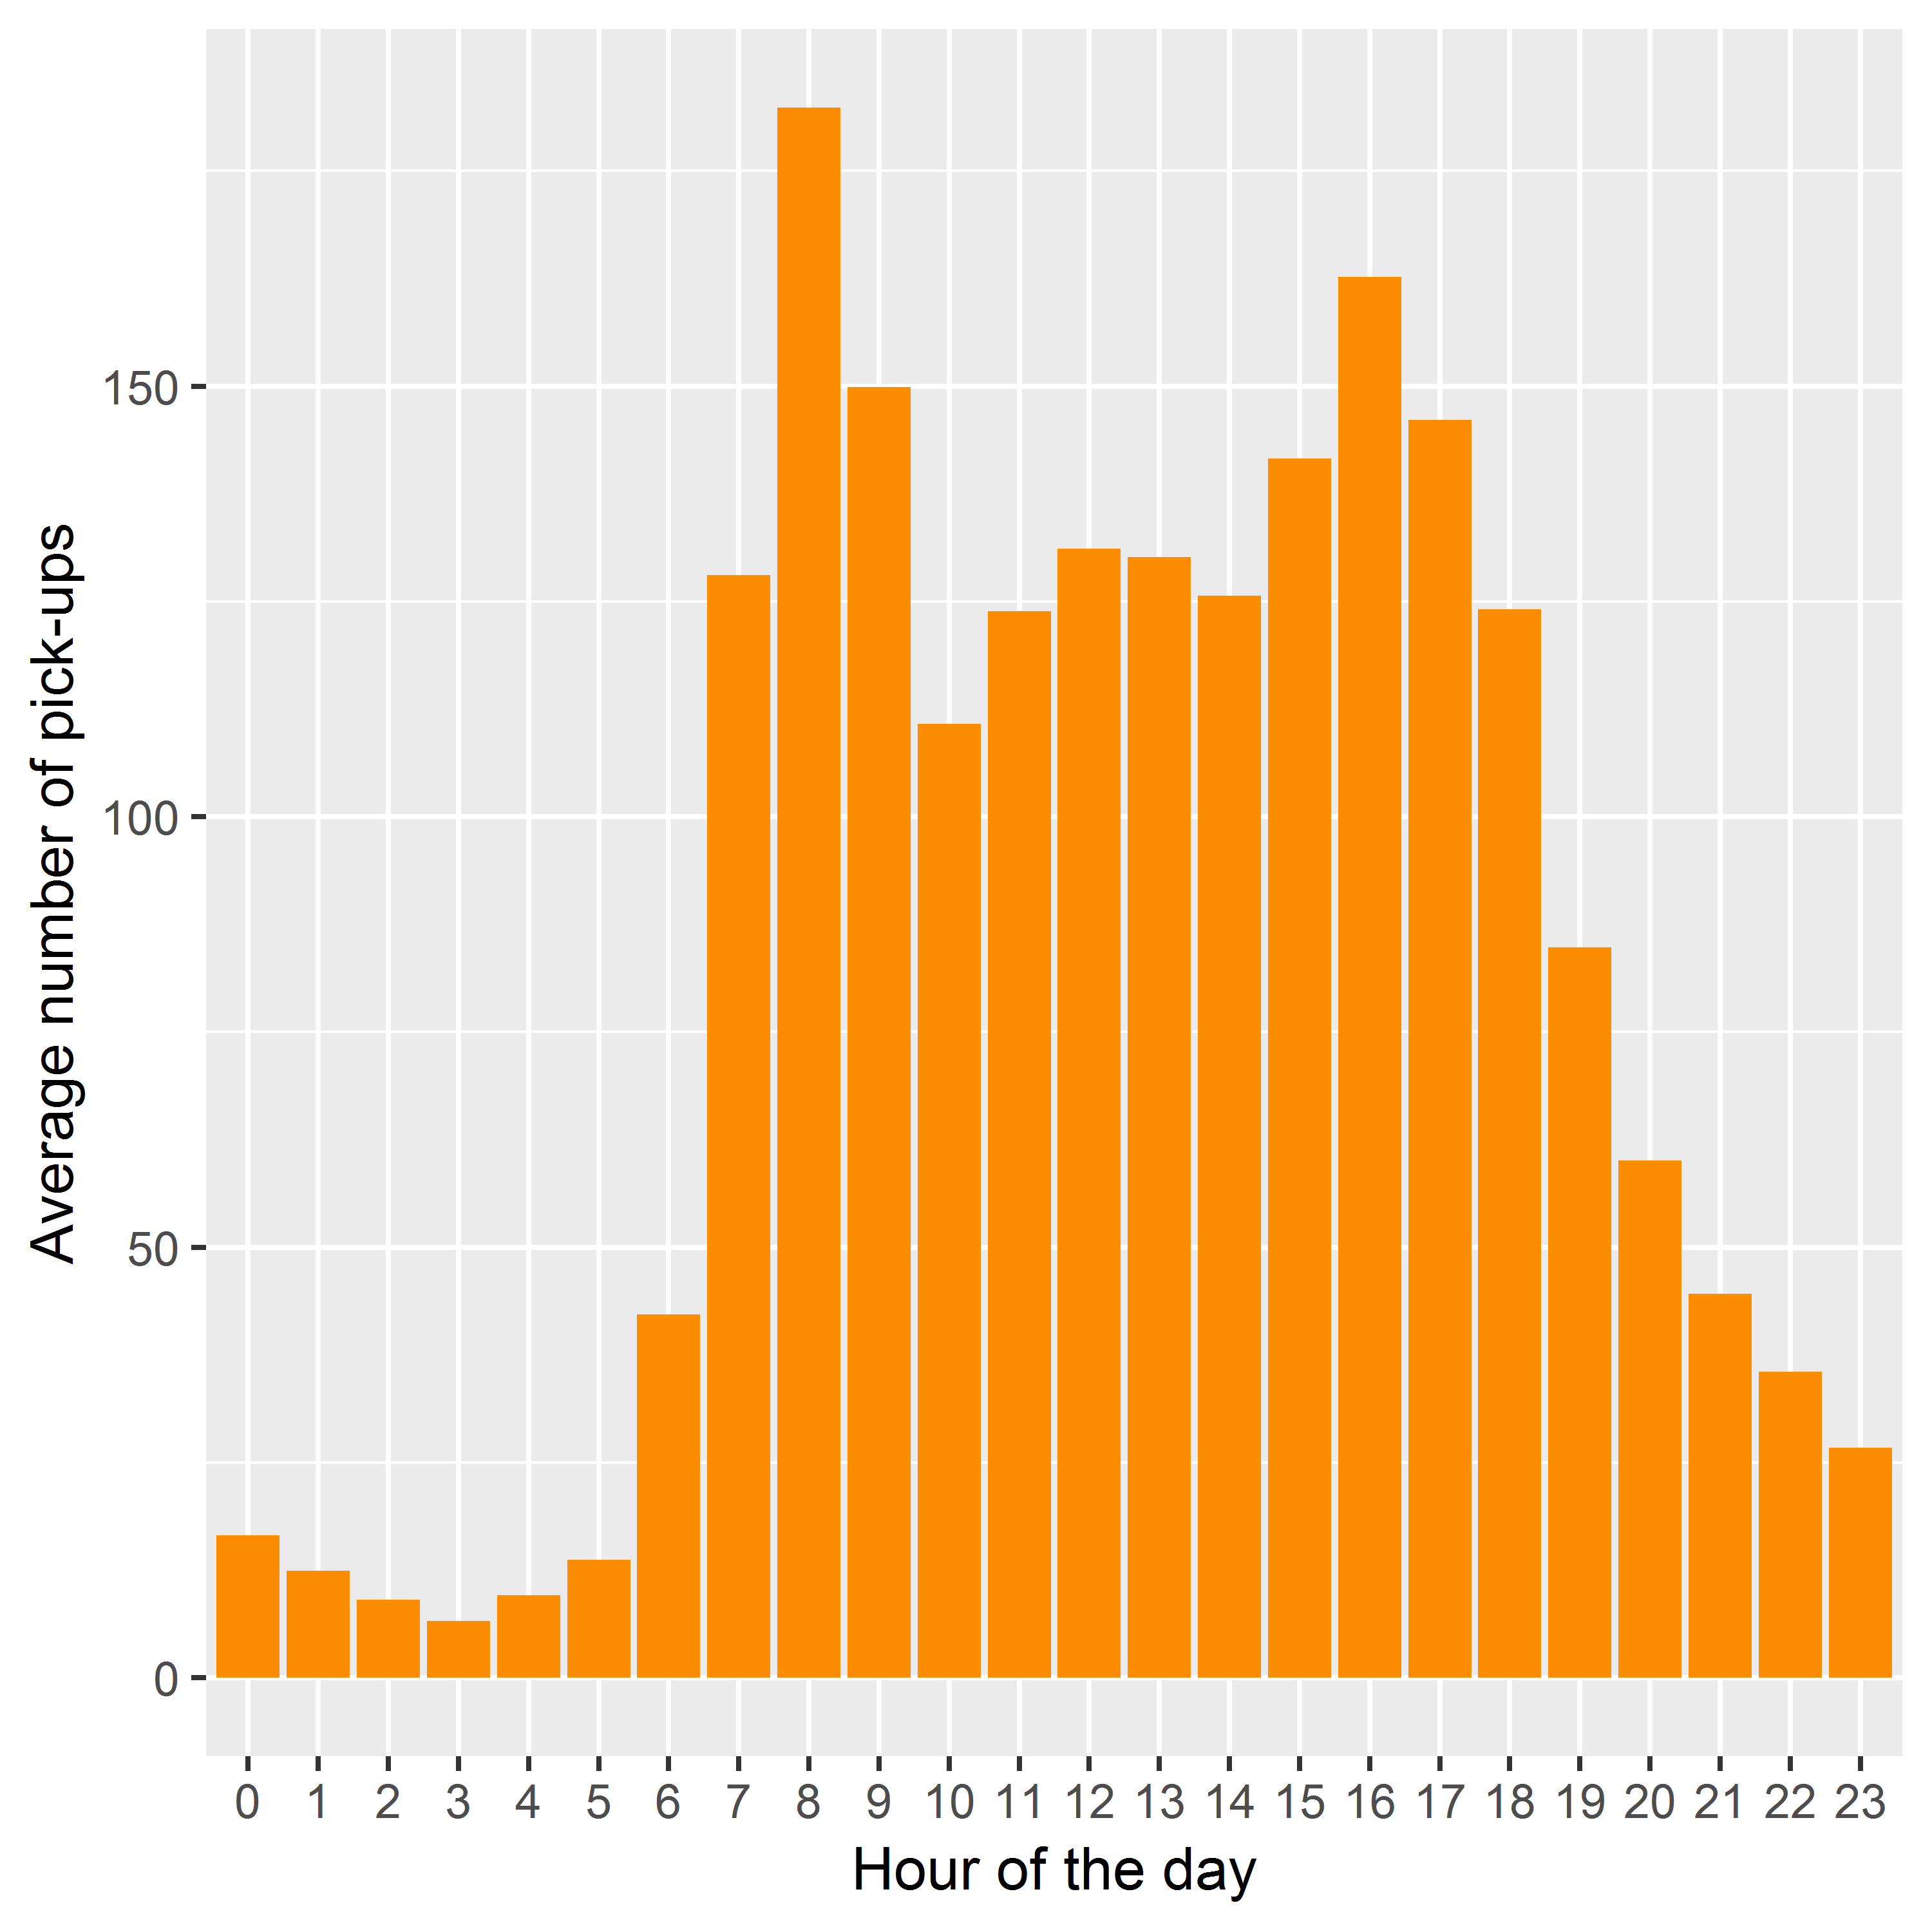
\includegraphics[width=0.5\linewidth]{Figures/usagehour} \caption{a) pick-ups per day of the week; b) pick-ups per hour of the day}\label{fig:usageplots}
\end{figure}
Recall that for each grid cell centroid, a time series of historical
distance data was queried, and that the normalized, average weekly
patterns in these data were clustered using spatially constrained
hierarchical clustering. The automatic procedure of defining the number
of clusters \(k\) and the mixing parameter \(\alpha\), lead to a
definition of \(k = 4\) and \(\alpha = 0.6\). This resulted in a
partition containing four fully spatial contiguous clusters. The
geographical outlines of these clusters are shown in Figure 5.2a. The
centroid of each cluster, weighted by the number of pick-ups in the
corresponding grid cells, are shown in Figure 5.2b. These weighted
centroids serve as the model points in DBAFS.
\begin{figure}[H]
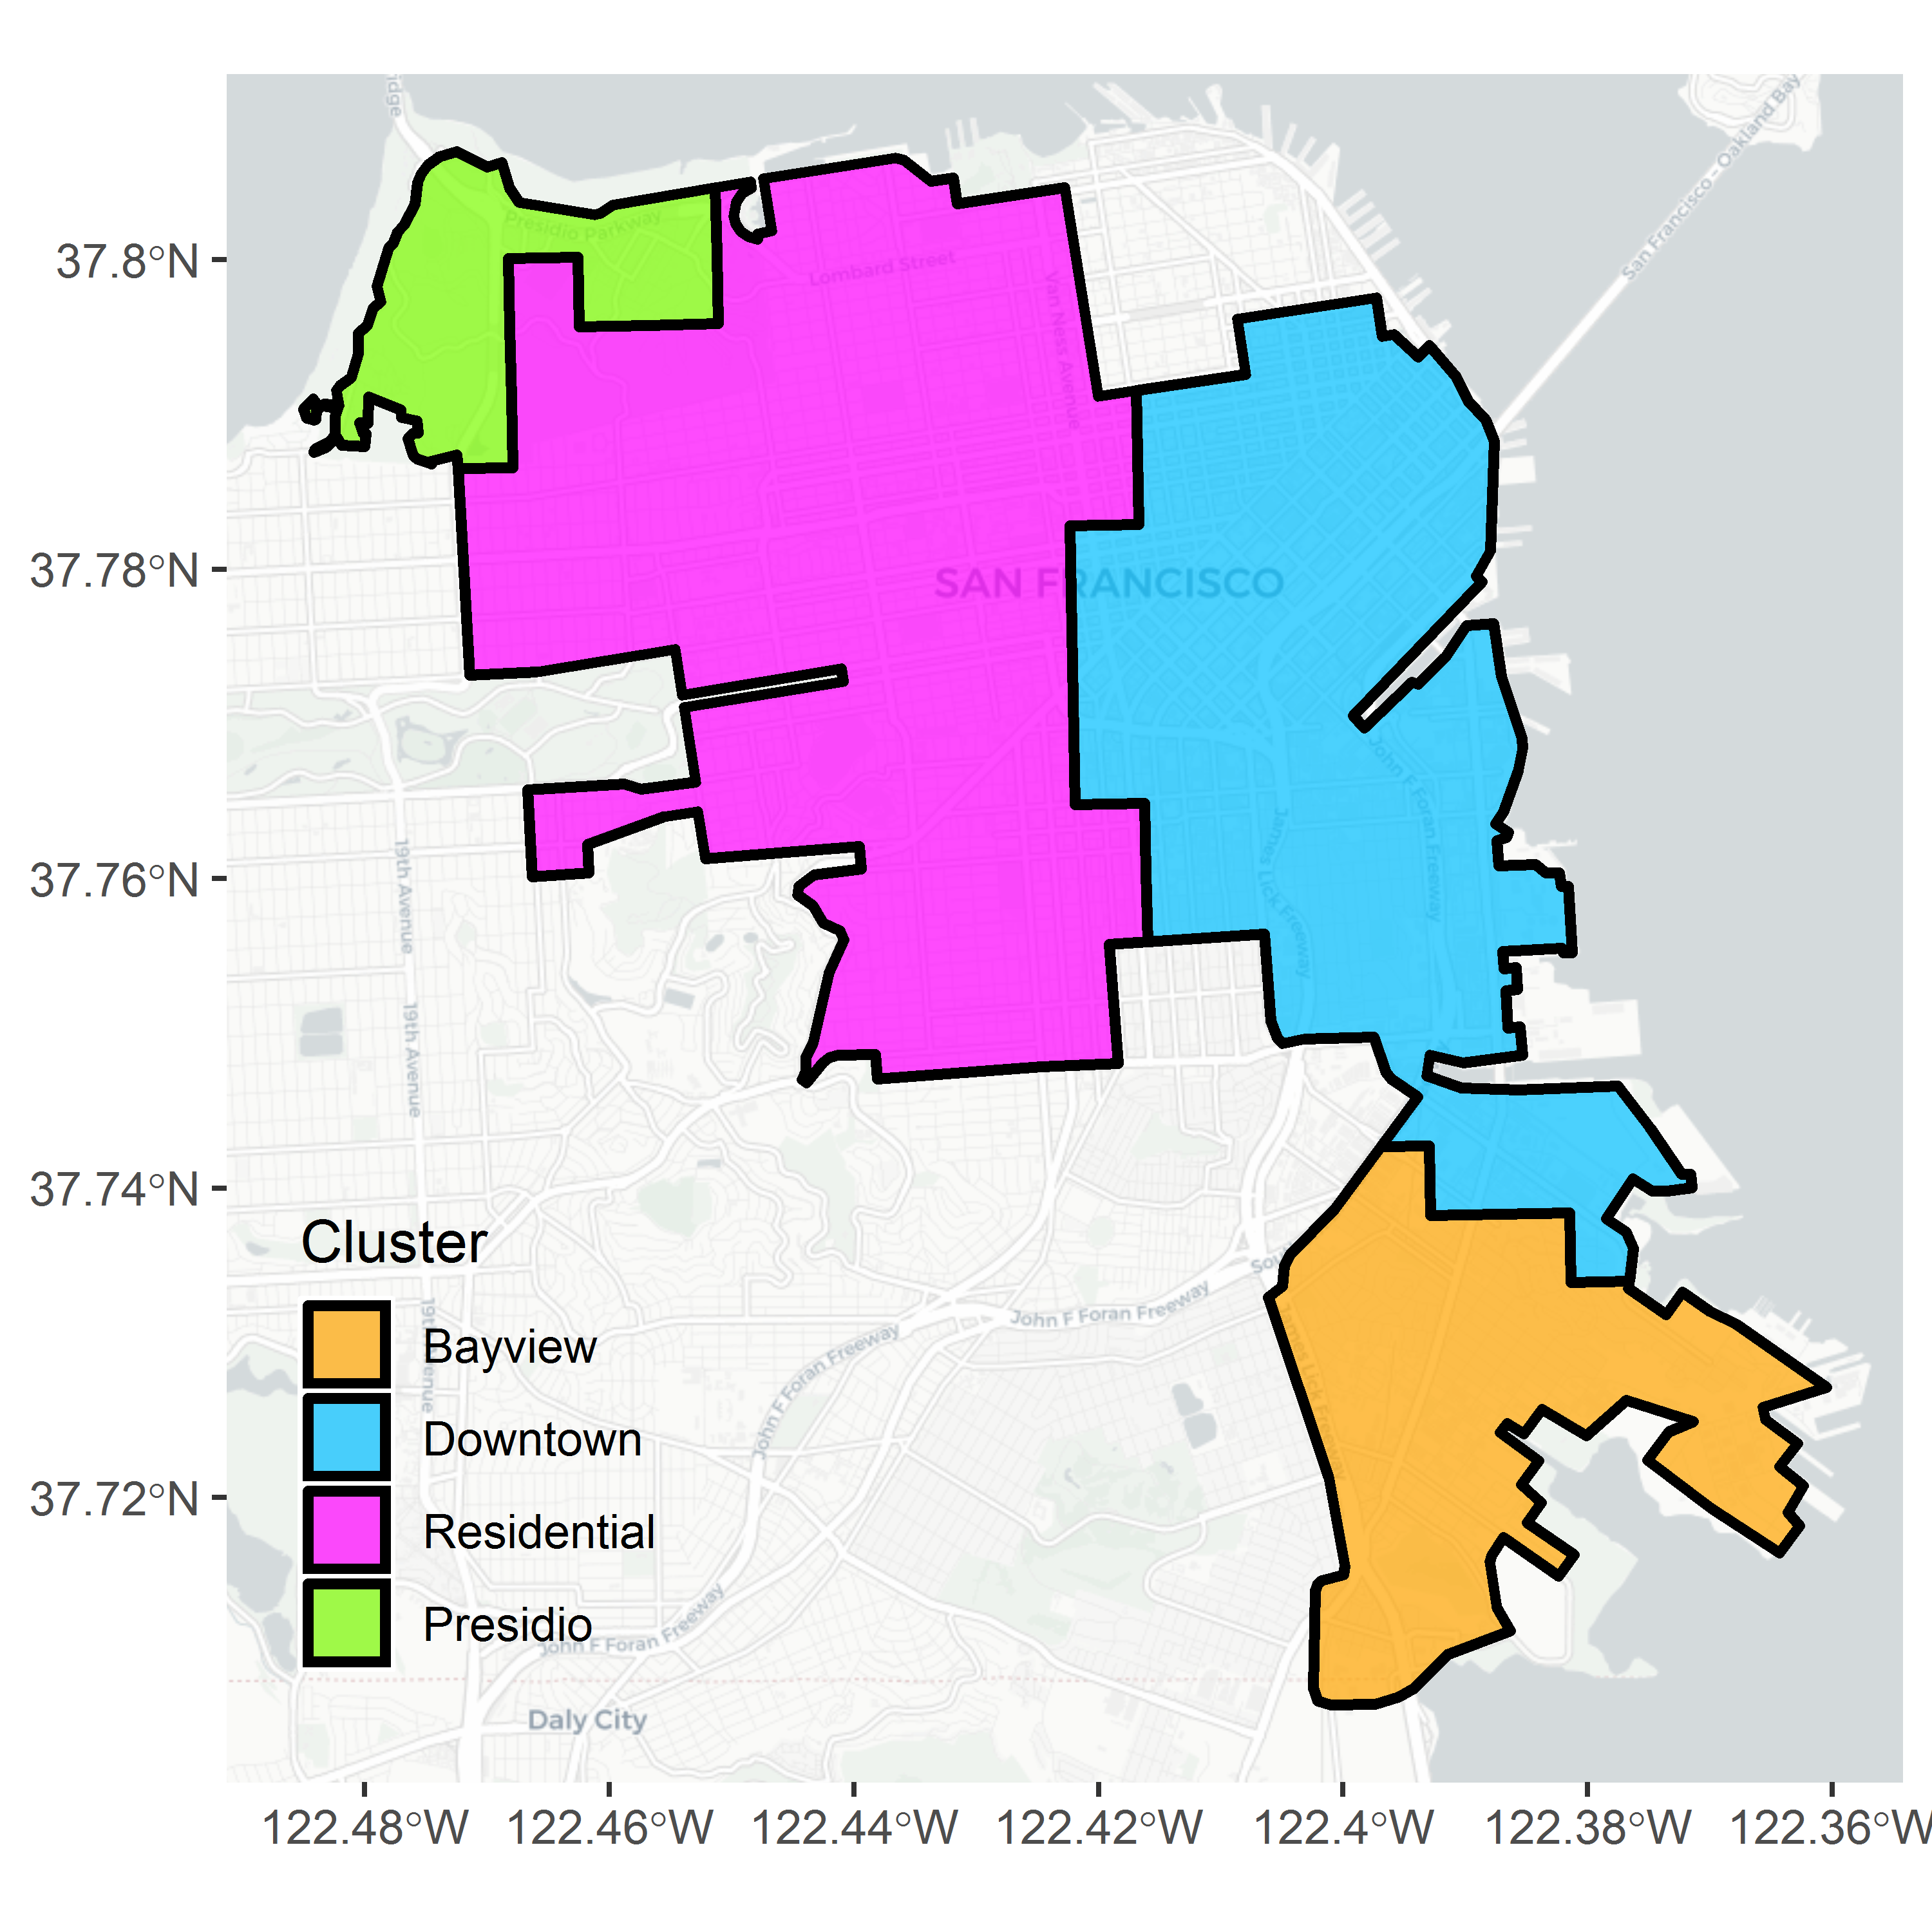
\includegraphics[width=0.5\linewidth]{Figures/clusters} 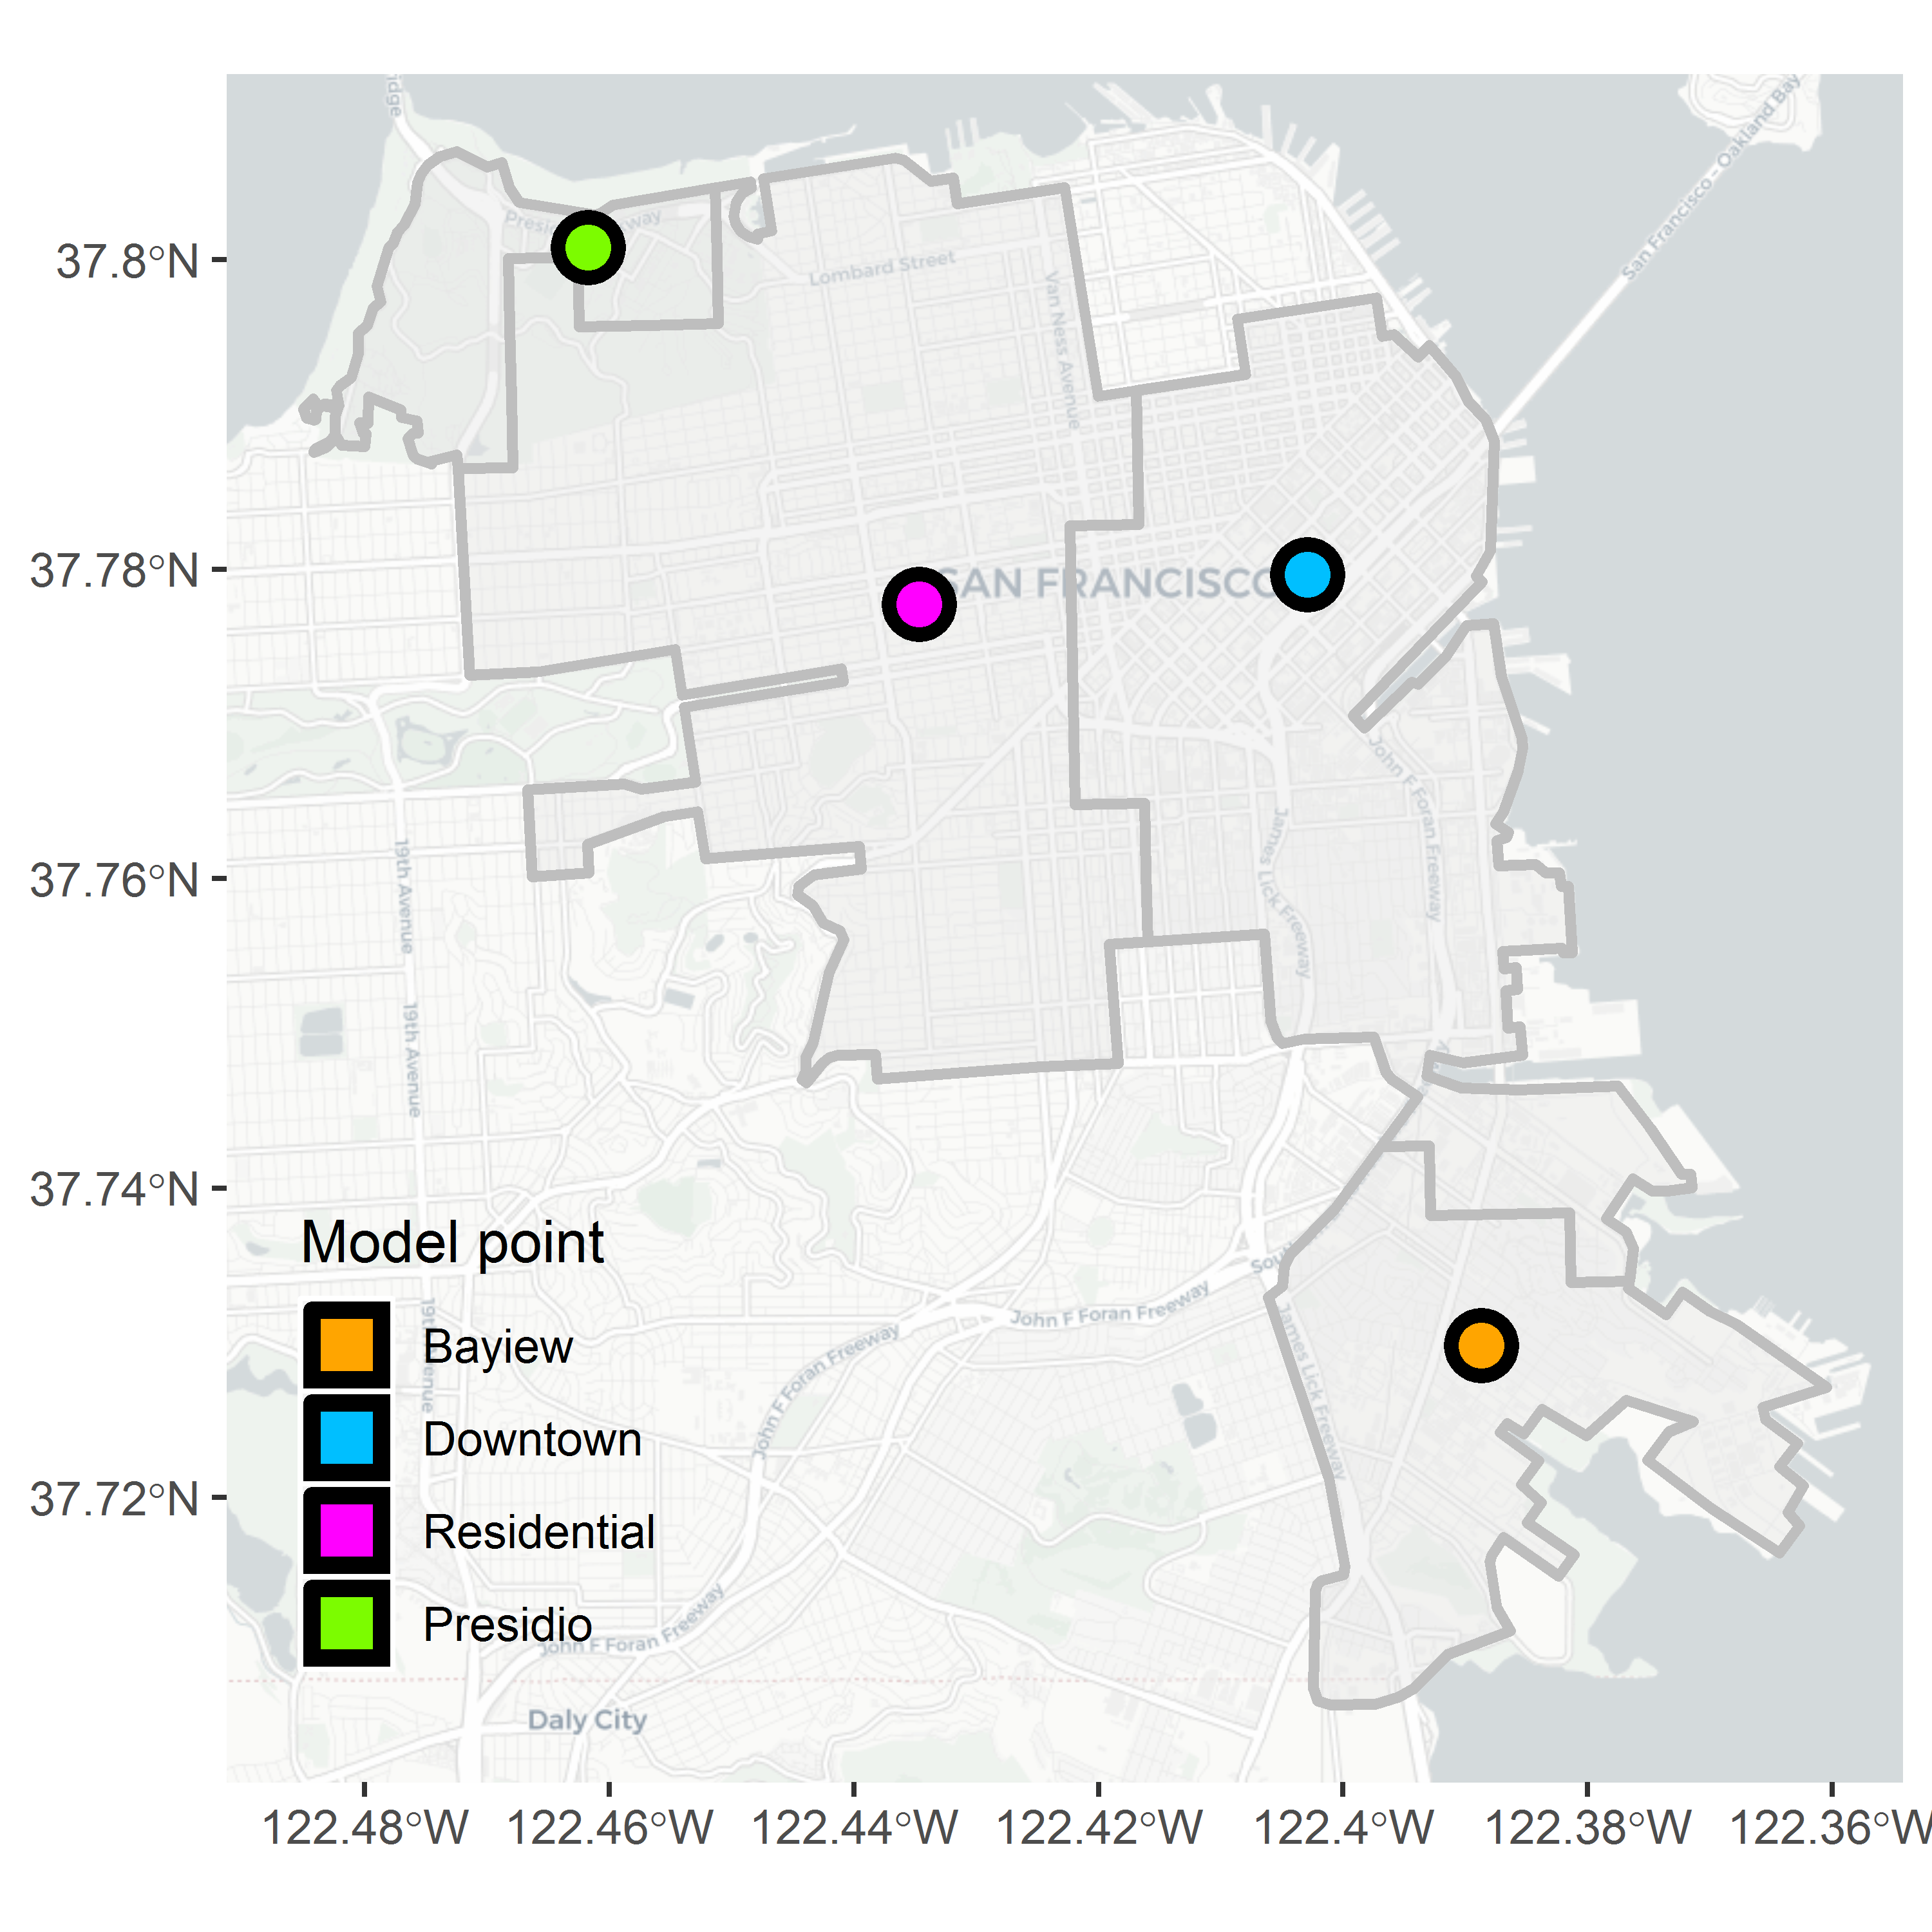
\includegraphics[width=0.5\linewidth]{Figures/modelpoints} \caption{a) cluster outlines; b) model point locations}\label{fig:clusters}
\end{figure}
Roughly speaking, and based on a large study of neighbourhood indicators
in San Francisco (San Francisco Department of Public Health,
\protect\hyperlink{ref-sfindicator}{2014}), the four clusters can be
characterized as follows. The orange cluster covers the Bayview/Hunters
Point neighbourhood, which is a rather isolated area, with a high
percentage of low-income households and relatively high crime rates. The
blue cluster forms the city center of San Francisco, containing the
neighbourhoods with the highest population densities, but also with a
relatively high job density compared to the residential density, and
large areas zoned for commercial usage. The purple cluster mainly
contains neighbourhoods where the residential density is high compared
to the job density, and the area zoned for commercial usage is
relatively small. Finally, the green cluster covers the Presidio Park, a
recreational area with few inhabitants, and a relatively high number of
bike lanes. For the sake of clarity, the orange, blue, purple and green
clusters are from now on referred to as the \emph{Bayview},
\emph{Downtown}, \emph{Residential} and \emph{Presidio} clusters,
respectively. Consistently, the four corresponding model points will be
called the \emph{Bayview}, \emph{Downtown}, \emph{Residential} and
\emph{Presidio} model points, respectively.

Table 1 presents some descriptive statistics of the time series,
averaged per cluster, and averaged over the whole system area. From the
249 grid cells, more than a hundred are located within the Residential
cluster, while the Presidio cluster is by far the smallest of the four.
During the training period, the nearest available bike was on average
located 619 meters from the grid cell centroids. In the Bayview cluster,
however, this was more than one kilometer, a difference of almost a
factor two compared to the Downtown cluster, and even more compared to
the Residential and Presidio clusters. The Bayview cluster also showed
the largest variation in the data, with a high average standard
deviation compared to the other clusters, and an average range that
spanned more than four kilometers. This can possibly be explained by the
low usage intensity of the bike sharing system in this part of the
system area. When the number of bikes in an area is low, the nearest
available bike and the second nearest available bike are more likely to
be far away from each other. In that case, when the closest of them gets
picked-up, the distance to the nearest available bike will suddenly
increase substantially. The other way around, when all available bikes
are far away, and one bike gets dropped-off inside the area, the
distance to the nearest available bike will suddenly decrease
substantially.

Although not as extreme as the Bayview cluster, also the other clusters
had on average high ranges when compared to the mean and standard
deviation. However, the standard deviation itself turned out to be
rather small relative to the range. This implies either the presence of
outliers, or population distributions with thin, but wide tails.

The first order autocorrelation measures the average dependency between
data values at time \(t\) and corresponding data values at time \(t-1\).
In the whole system area, this dependency was strong, especially in the
Bayview and Presidio clusters. These high autocorrelation values are
important, since they imply that it is reasonable to use past
observations when forecasting future ones. However, the calculated
spectral entropy values show that in general, the data are also very
complex, and the forecastability is low. This mainly concerns the
Downtown and Residential clusters, which contain, as could be seen in
Figure 5.1b, the areas where the pick-up density is high. In such areas,
the data are more dynamic, since bikes get picked-up and dropped off
constantly, and the location of the nearest available bike will change
often. In most cases, the more dynamic the data, the harder to forecast.
\begin{table}[H]

\caption{\label{tab:clusterstats}Descriptive statistics of the grid cell centroids distance data}
\centering
\begin{tabular}{>{\bfseries\raggedright\arraybackslash}p{4cm}>{\raggedright\arraybackslash}p{1.5cm}>{\raggedright\arraybackslash}p{1.5cm}>{\raggedright\arraybackslash}p{1.5cm}>{\raggedright\arraybackslash}p{1.5cm}>{\raggedright\arraybackslash}p{1.5cm}>{\raggedright\arraybackslash}p{1.5cm}}
\toprule
  & $N$ & $\mu$ & $range$ & $\sigma$ & $\rho(1)$ & $H$\\
\midrule
\rowcolor{gray!6}  Total & 249 & 619 & 2726 & 422 & 0.82 & 0.77\\
Bayview & 46 & 1080 & 4021 & 631 & 0.95 & 0.67\\
\rowcolor{gray!6}  Downtown & 81 & 557 & 2551 & 352 & 0.77 & 0.81\\
Residential & 103 & 490 & 2410 & 371 & 0.79 & 0.81\\
\rowcolor{gray!6}  Presido & 19 & 462 & 2057 & 310 & 0.92 & 0.68\\
\bottomrule
\multicolumn{7}{l}{\textit{\scriptsize{Except $N$, all metrics are calculated for each time series seperately, and averaged afterwards.}}}\\
\multicolumn{7}{l}{\textsuperscript{1} \scriptsize{$N$ is the total number of grid cell centroids}}\\
\multicolumn{7}{l}{\textsuperscript{2} \scriptsize{$\mu$ is the mean of the data, in meters}}\\
\multicolumn{7}{l}{\textsuperscript{3} \scriptsize{$range$ is the difference between the maximum and minimum data value, in meters}}\\
\multicolumn{7}{l}{\textsuperscript{4} \scriptsize{$\sigma$ is the standard deviation of the data, in meters}}\\
\multicolumn{7}{l}{\textsuperscript{5} \scriptsize{$\rho(1)$ is the first order autocorrelation, see section 2.2.1}}\\
\multicolumn{7}{l}{\textsuperscript{6} \scriptsize{$H$ is the normalized spectral entropy, see section 2.2.3}}\\
\end{tabular}
\end{table}
Figure 5.3 shows the normalized, average weekly patterns of the time
series, averaged once again per cluster. The patterns can be explained
intuitively. The Bayview cluster has a low usage intensity, and although
there are peaks in the data every day, a clear and consistent pattern is
absent. The Downtown cluster has a high density of jobs and commercial
activities. During working hours, the demand for bikes is low, which
leads to a high number of available bikes, and consequently, short
distances to the nearest available bike. In the afternoon, just after
working hours, the demand starts increasing, and it gets harder to find
an available bike nearby. This peak in the data continues during the
evening, when the activity in the commericial zones is high. Later in
the evening, the demand decreases again. However, the data lacks a clear
peak during morning peak hours, as well as a clear difference between
weekdays and weekends, indicating that there is a substantial share of
non-commute related usage.

The Residential cluster shows the exact opposite pattern. In the morning
rush hours, commuters use the bike to get to work, and not many
available bikes are left in the residential areas. Hence, in those
areas, the distance to the nearest available bike is higher during
working hours. In the afternoon, commuters come back from work, and
leave the bikes in the residential areas, causing a decrease in distance
to the nearest available bike. Hence, the distance data peaks during
working hours. In the weekends, the peaks seem to be slightly lower, but
this difference is not as large as might have been expected. They do
happen later on the day, corresponding to the same periods as the
Downtown cluster.

Finally, the Presidio cluster is mainly a recreational area. There are a
lot of bikes, but during weekdays, they are used less, leading to small
and relatively constant distances to the nearest available bike. In
weekends, and mainly on Sunday afternoon, the usage intensity is high,
and it takes longer to find an available bike.
\begin{figure}[H]
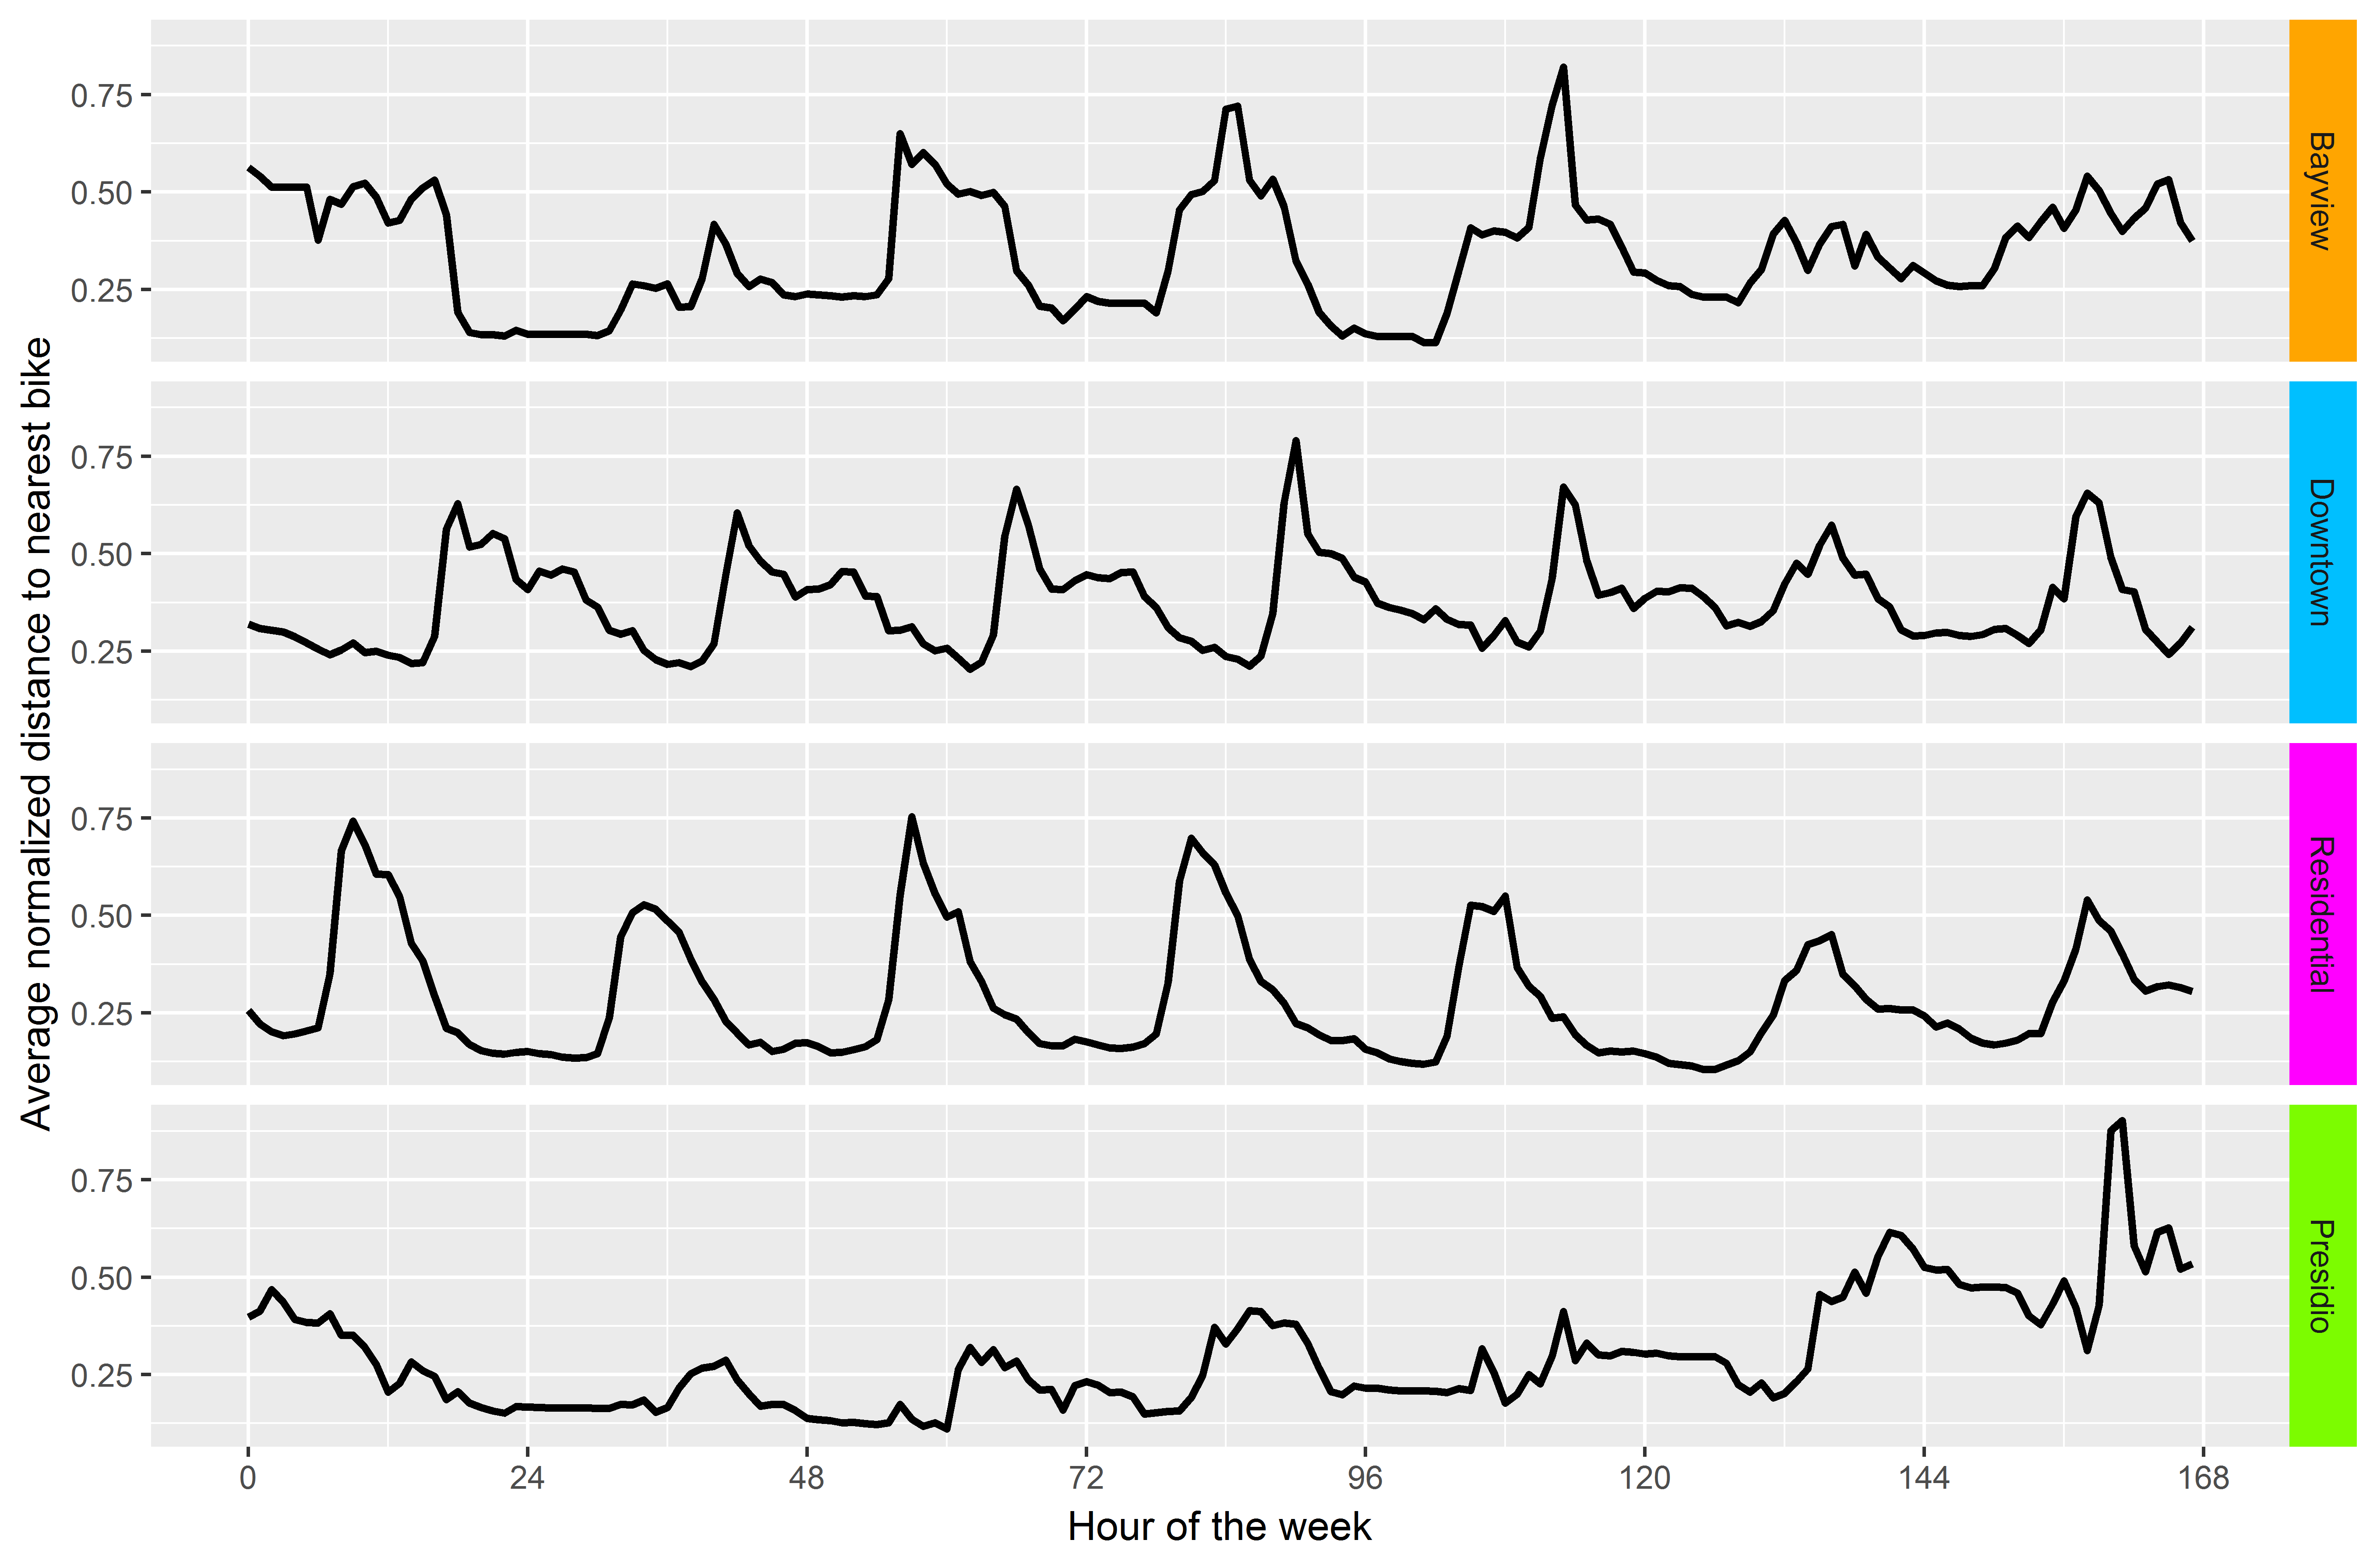
\includegraphics[width=\textwidth]{Figures/clusterplots} \caption{Patterns of the distance data for the grid centroids, per cluster}\label{fig:patterns}
\end{figure}
\section{Model building}\label{model-building}

Figure 5.4 shows the time plots of the distance data that were queried
for each of the model points in Figure 5.2b, with the dark grey shaded
areas representing weekends. The plots endorse the findings in the
previous sections. The data corresponding to the Bayview model point
show large variation, interspersed with flat sections, and lack a clear
repeating pattern. The data corresponding to the Downtown and
Residential model points are most dynamic. A daily pattern shows for
both of them. However, in both datasets, this pattern is far from
smooth, and the daily peaks vary considerably in height from day to day.
This underlines the high spectral entropies that were found for these
clusters. A clear difference between weekdays and weekends, can not be
seen. The Presidio model point shows the most constant data, with a low
mean and long flat sections. Sunday afternoons stand out clearly in most
of the weeks, but not in all of them. The last sunday, for example,
shows only a minor peak in the data. In less extent, this also applies
to the other clusters, with lower peaks than normal, in the last
weekend. Finally, none of the datasets contain missing values, and clear
evidence for non-constant variances is not present.
\begin{figure}[H]
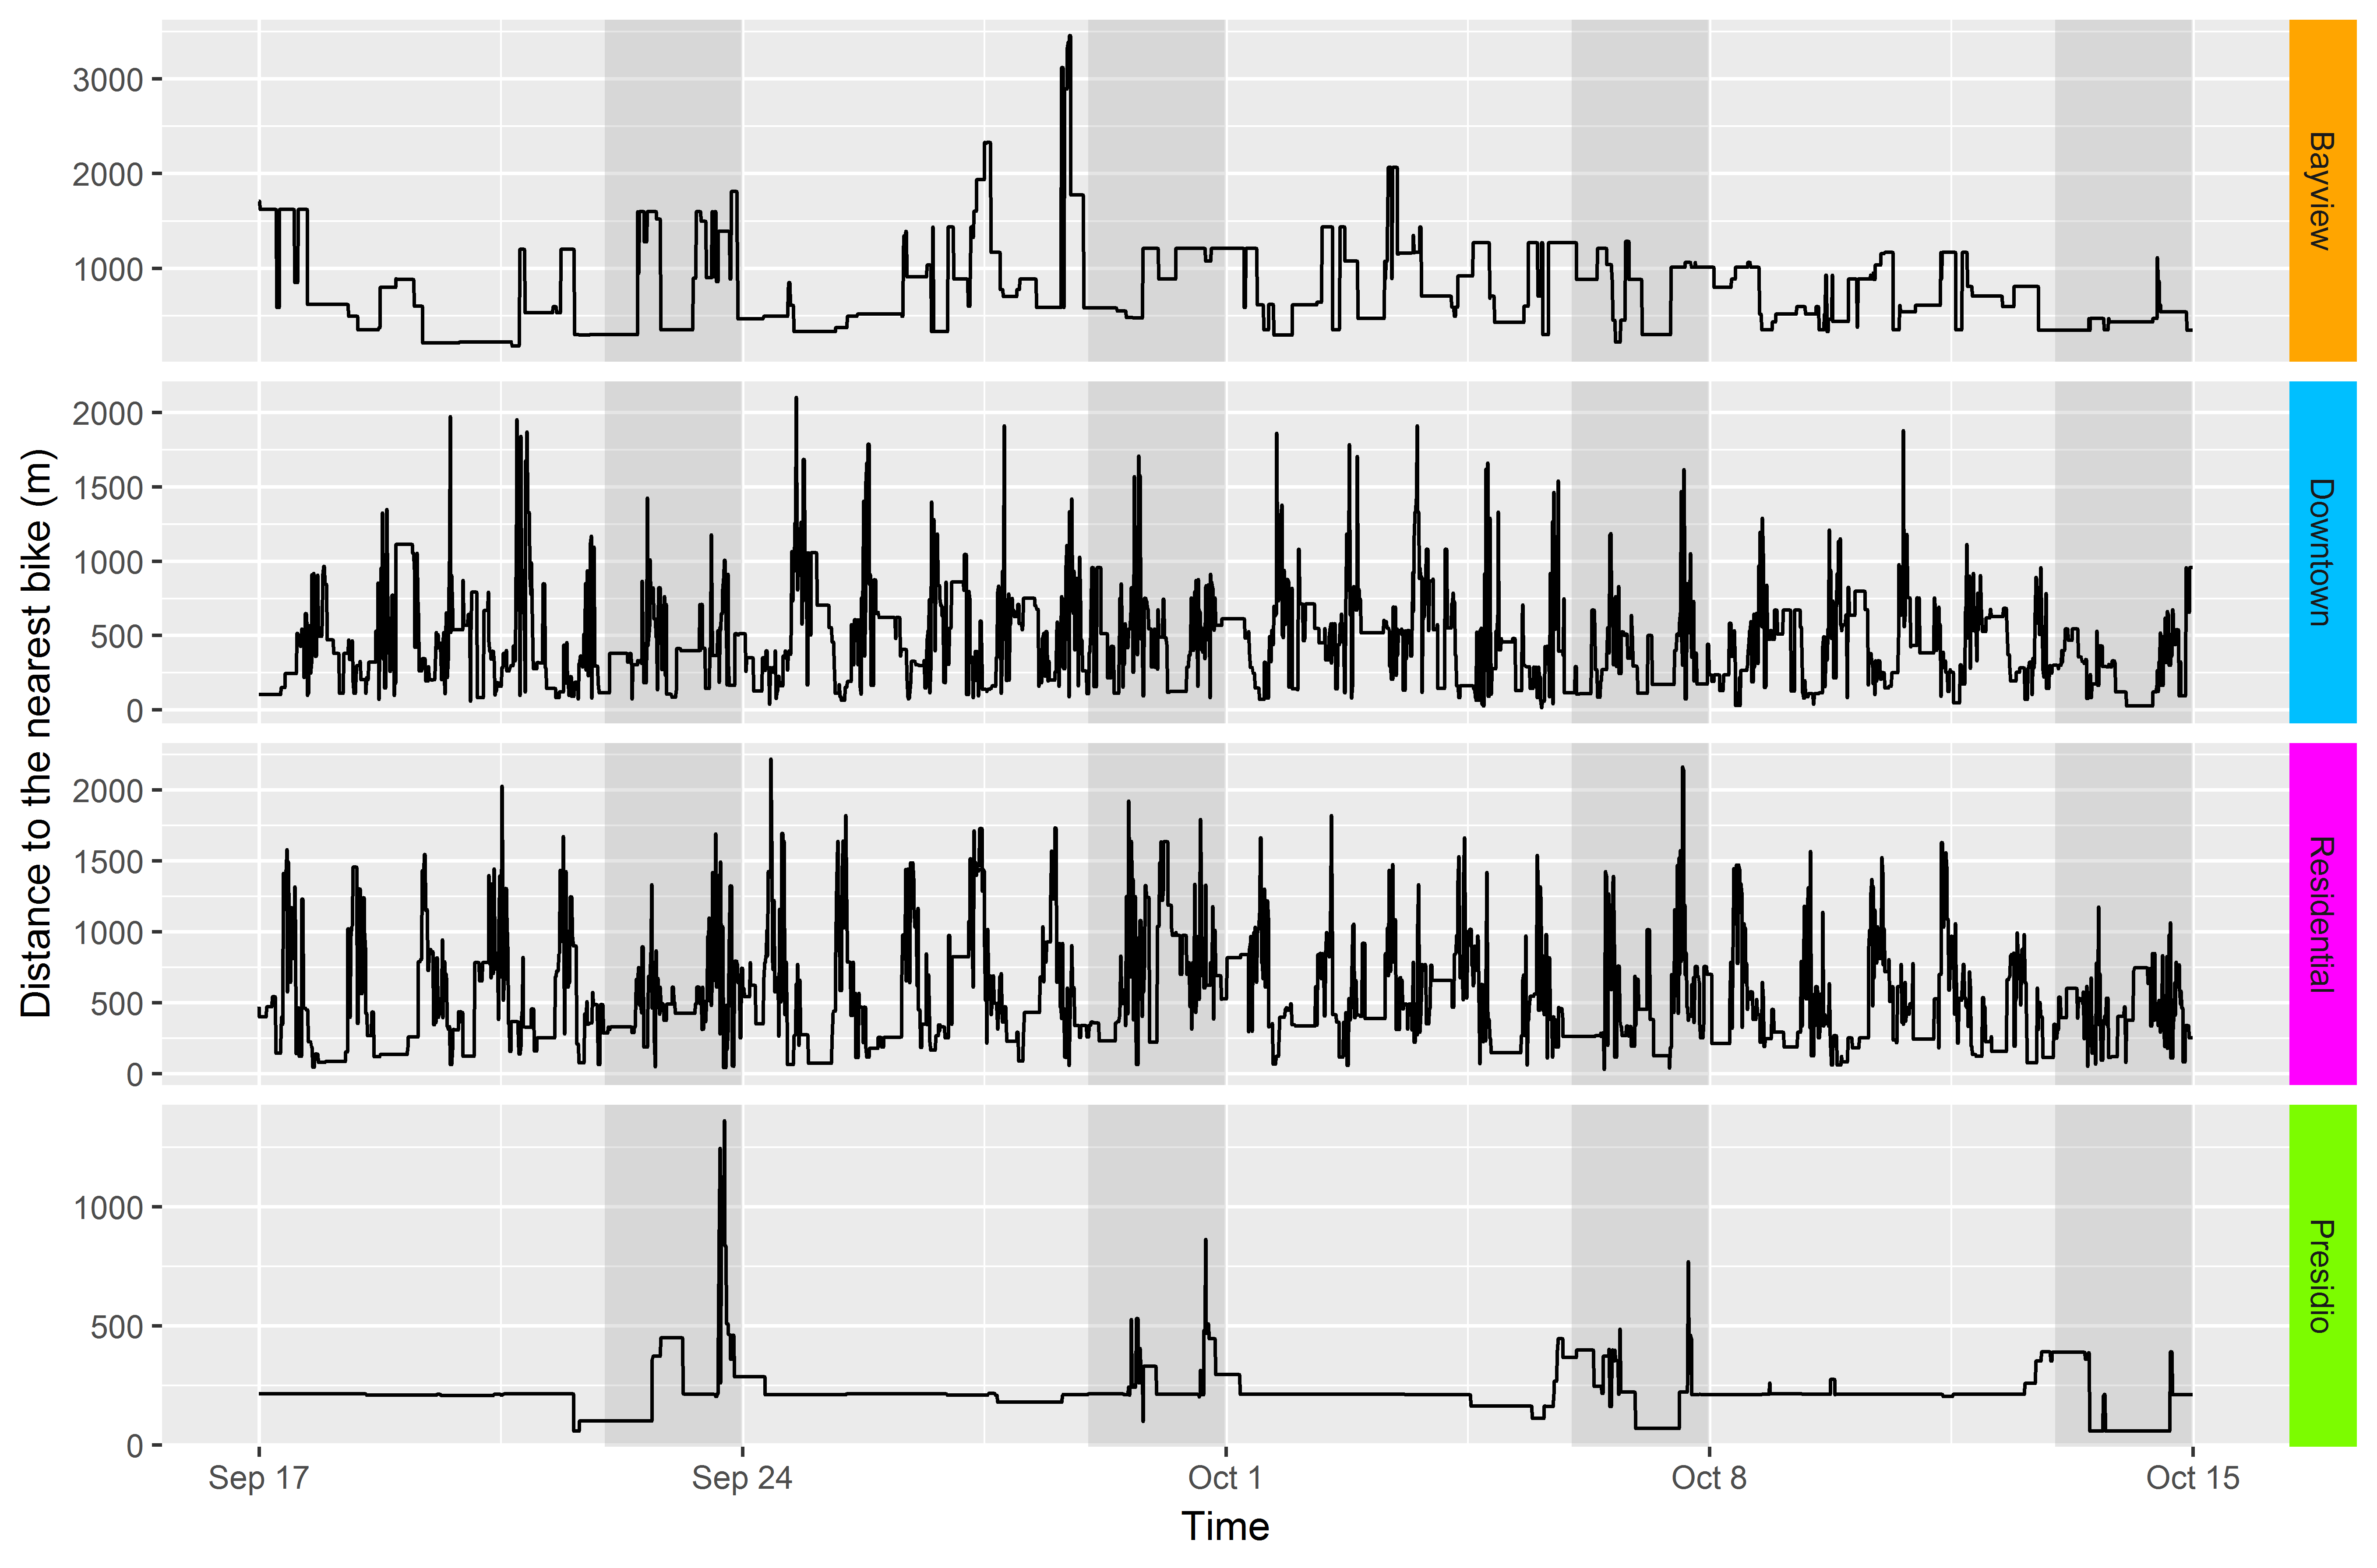
\includegraphics[width=\textwidth]{Figures/timeplots} \caption{Time plots of the distance data for the model points}\label{fig:timeplots}
\end{figure}
The structures of the fitted models are shown in Table 5.2. The
automatic seasonality detection resulted in a daily seasonal pattern for
both the Downtown and the Residential model point. As expected, a weekly
seasonal pattern was found for the Presidio model point, an no
seasonality for the Bayview model point. The ARIMA(\(p\), \(d\), \(q\))
models for the Bayview and Downtown model points, have a relatively high
number of autoregressive terms, while for the Presidio model point, the
number of moving average terms is high. For the Residential model point,
the best fit was obtained by only including one autoregressive and one
moving average term. All datasets passed the KPSS test for stationarity
after one differencing operation. The full details of the components and
fitted models, including parameter estimates and decomposition plots,
can be found in Appendix B.
\begin{table}[H]

\caption{\label{tab:modelstructure}Model structures}
\centering
\begin{tabular}{>{\bfseries\raggedright\arraybackslash}p{4cm}>{\centering\arraybackslash}p{3cm}>{\centering\arraybackslash}p{1.5cm}>{\centering\arraybackslash}p{1.5cm}>{\centering\arraybackslash}p{1.5cm}}
\toprule
  & seasonality & $p$ & $d$ & $q$\\
\midrule
\rowcolor{gray!6}  Bayview & none & 3 & 1 & 1\\
Downtown & daily & 3 & 1 & 2\\
\rowcolor{gray!6}  Residential & daily & 1 & 1 & 1\\
Presidio & weekly & 1 & 1 & 4\\
\bottomrule
\end{tabular}
\end{table}
Figure 5.5 shows the residuals of each model, plotted over time. All
models have residuals with an approximately zero mean, and the variances
look approximately constant. Comparing Figure 5.5 with Figure 5.4, it
can be seen that for the less dynamic data in Bayview and Presidio, the
models struggle to find a good fit for the peaks and valleys in the
data, while the flat sections are explained accurately.
\begin{figure}[H]
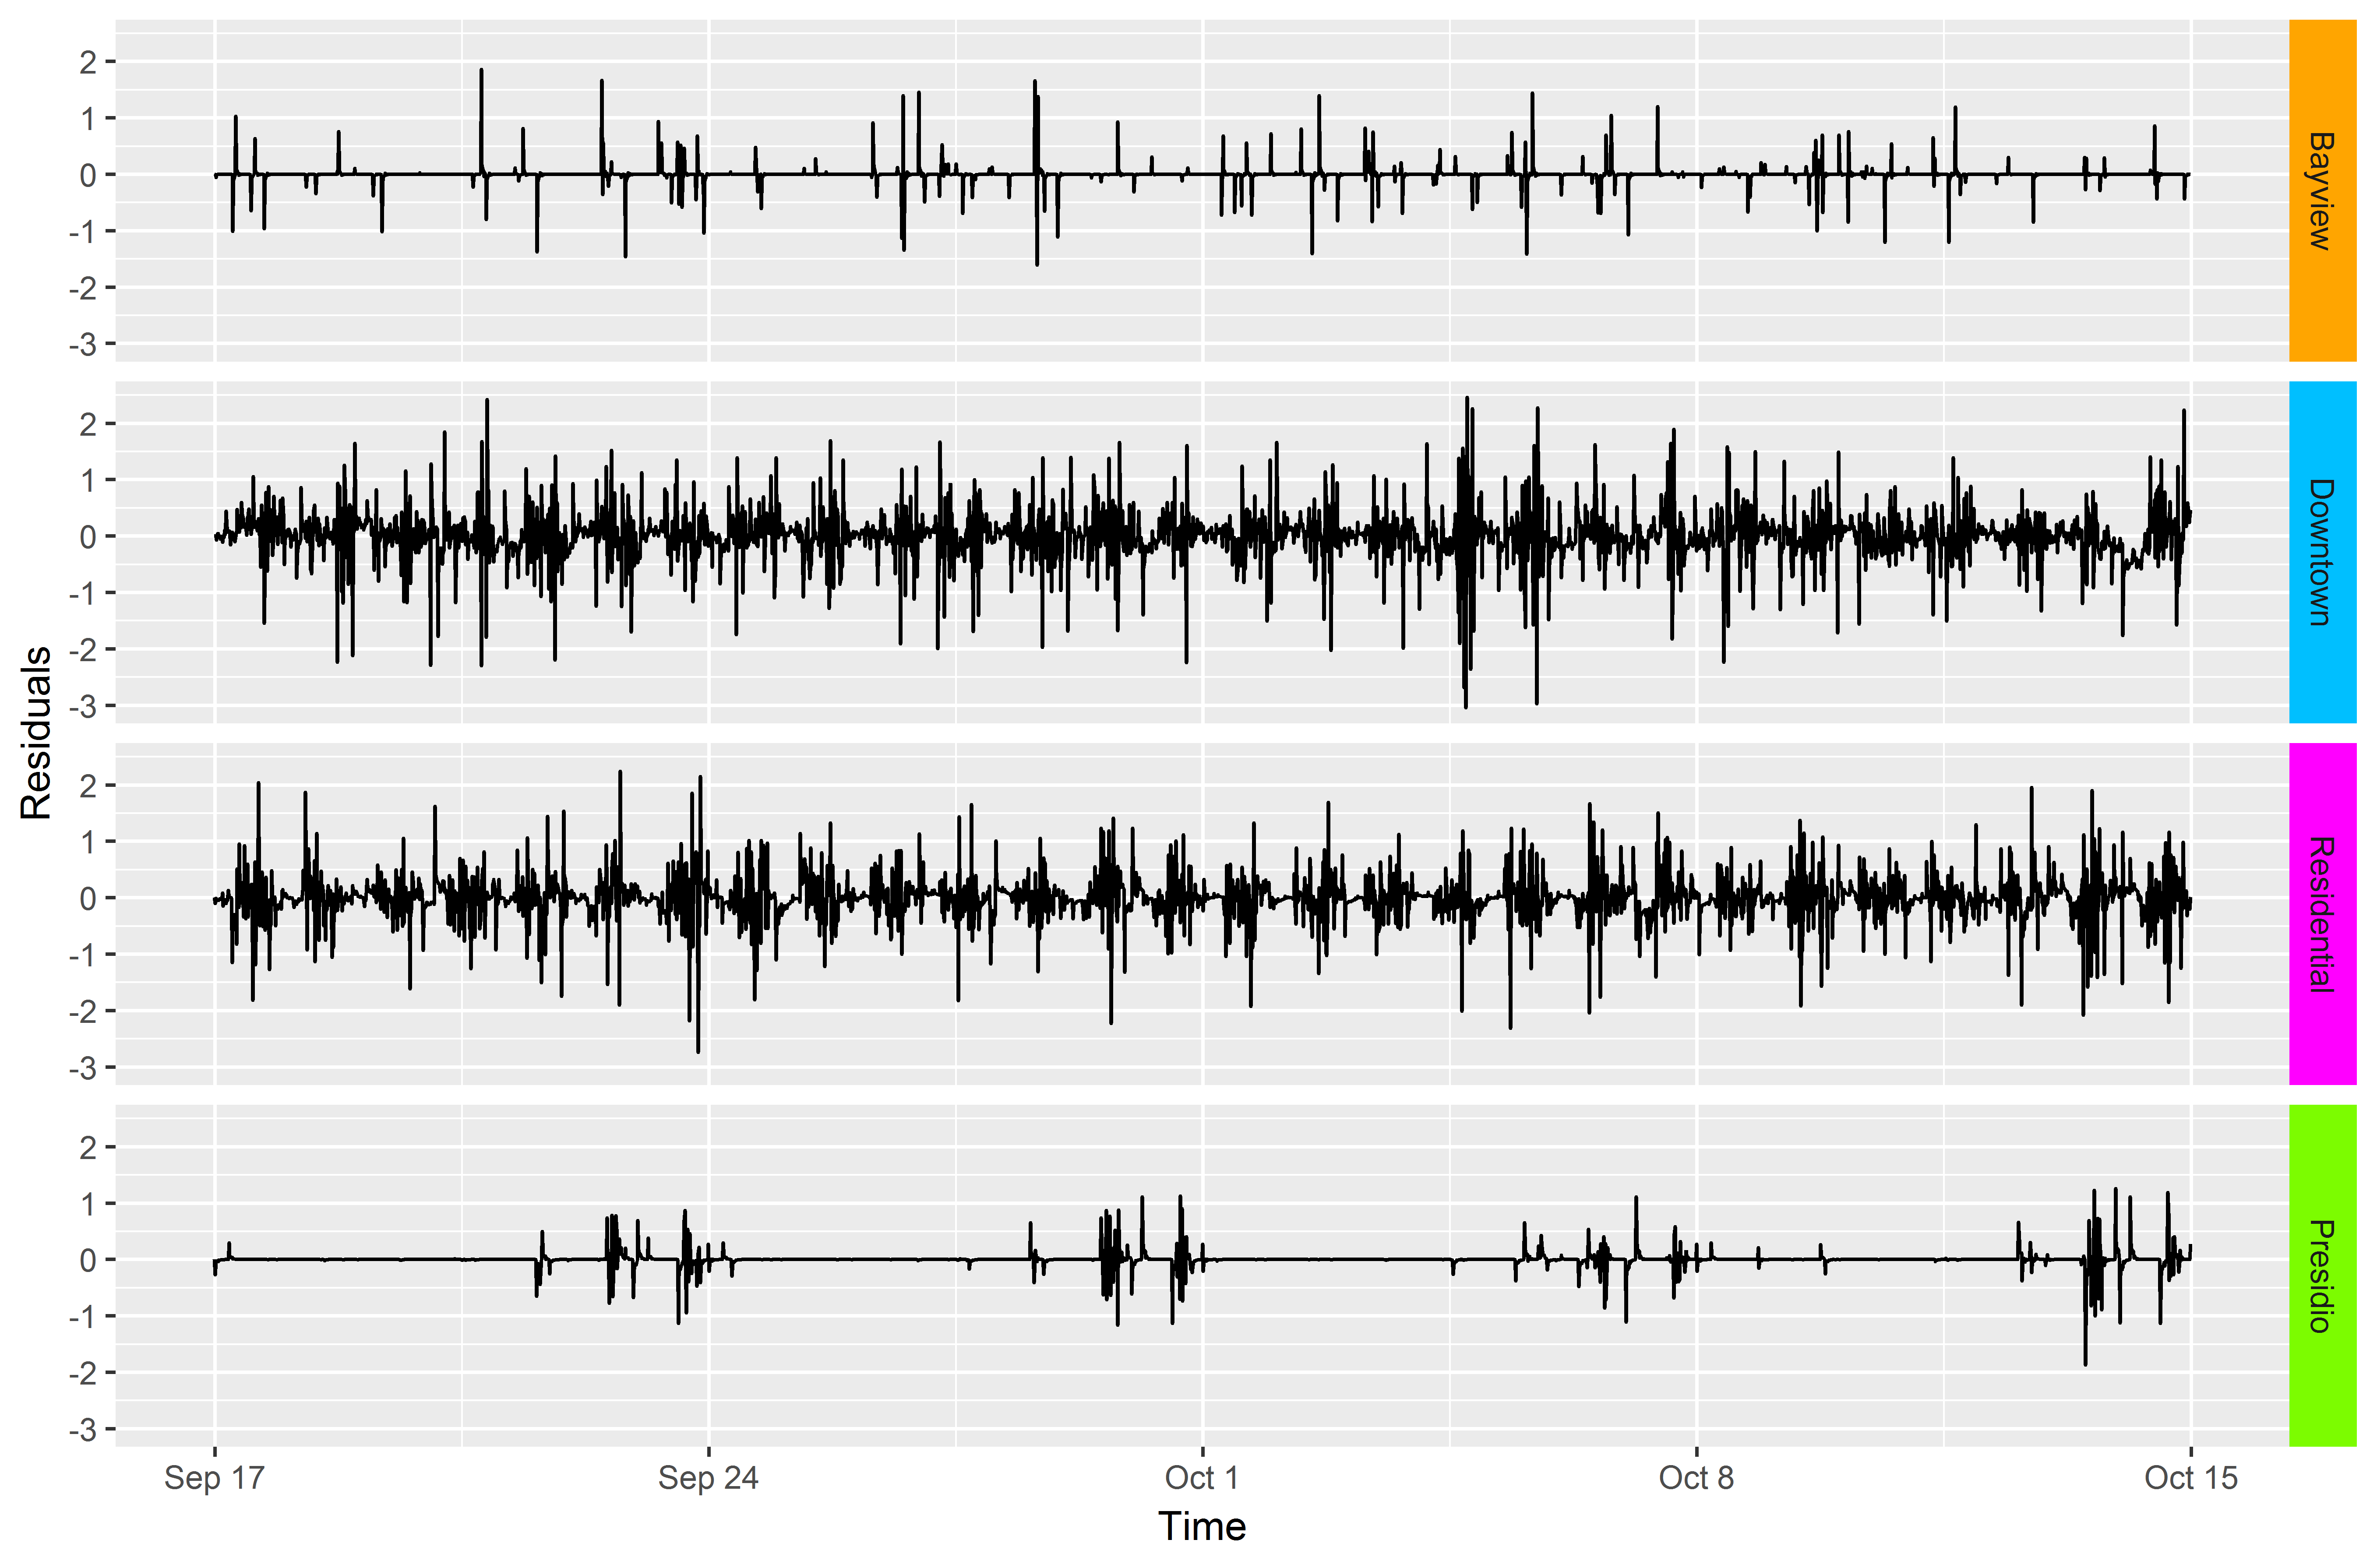
\includegraphics[width=\textwidth]{Figures/residual_timeplots} \caption{Time plots of the model residuals}\label{fig:residualtimeplots}
\end{figure}
The autocorrelations at several time lags in the residuals are shown in
Figure 5.6. Since the data have a temporal resolution of 15 minutes, 96
time lags correspond to one day, and 672 time lags, the total span of
the x-axis in the figure, to one week. The dotted orange lines form the
lower and upper 95\% confidence bounds, assuming a normal distribution.
This means that the residuals are considered to be a realization of a
white noise process when at least 95\% of the autocorrelation values
fall within these bounds. It is important to note here that when working
with real-world data, finding perfectly random model residuals is an
exception, especially when the data have a high entropy. Taking that
into account, the autocorrelation plot of the Bayview, Downtown and
Residential models look good, and their residuals seem to approximate
white noise.

However, for the Presidio cluster, the residual autocorrelation has a
strong peak at lag 672, corresponding to one week. Recall that the data
of the Presidio model point was relatively flat during the weekdays, and
spiky in the weekends. These spikes, however, varied considerably in
amplitude from week to week. The weekly seasonal component that was
substracted from the data, accounts for the recurring patterns, but can
not completely capture the differences from week to week. Therefore,
errors during the `spiky' weekends, will still be higher than during the
`flat' weekdays, causing autocorrelation in the residuals. With just a
stochastic time series model, it is hard to solve this. Including
external variables that explain the variation, could be an option, and
will be discussed in section 5.4.2.
\begin{figure}[H]
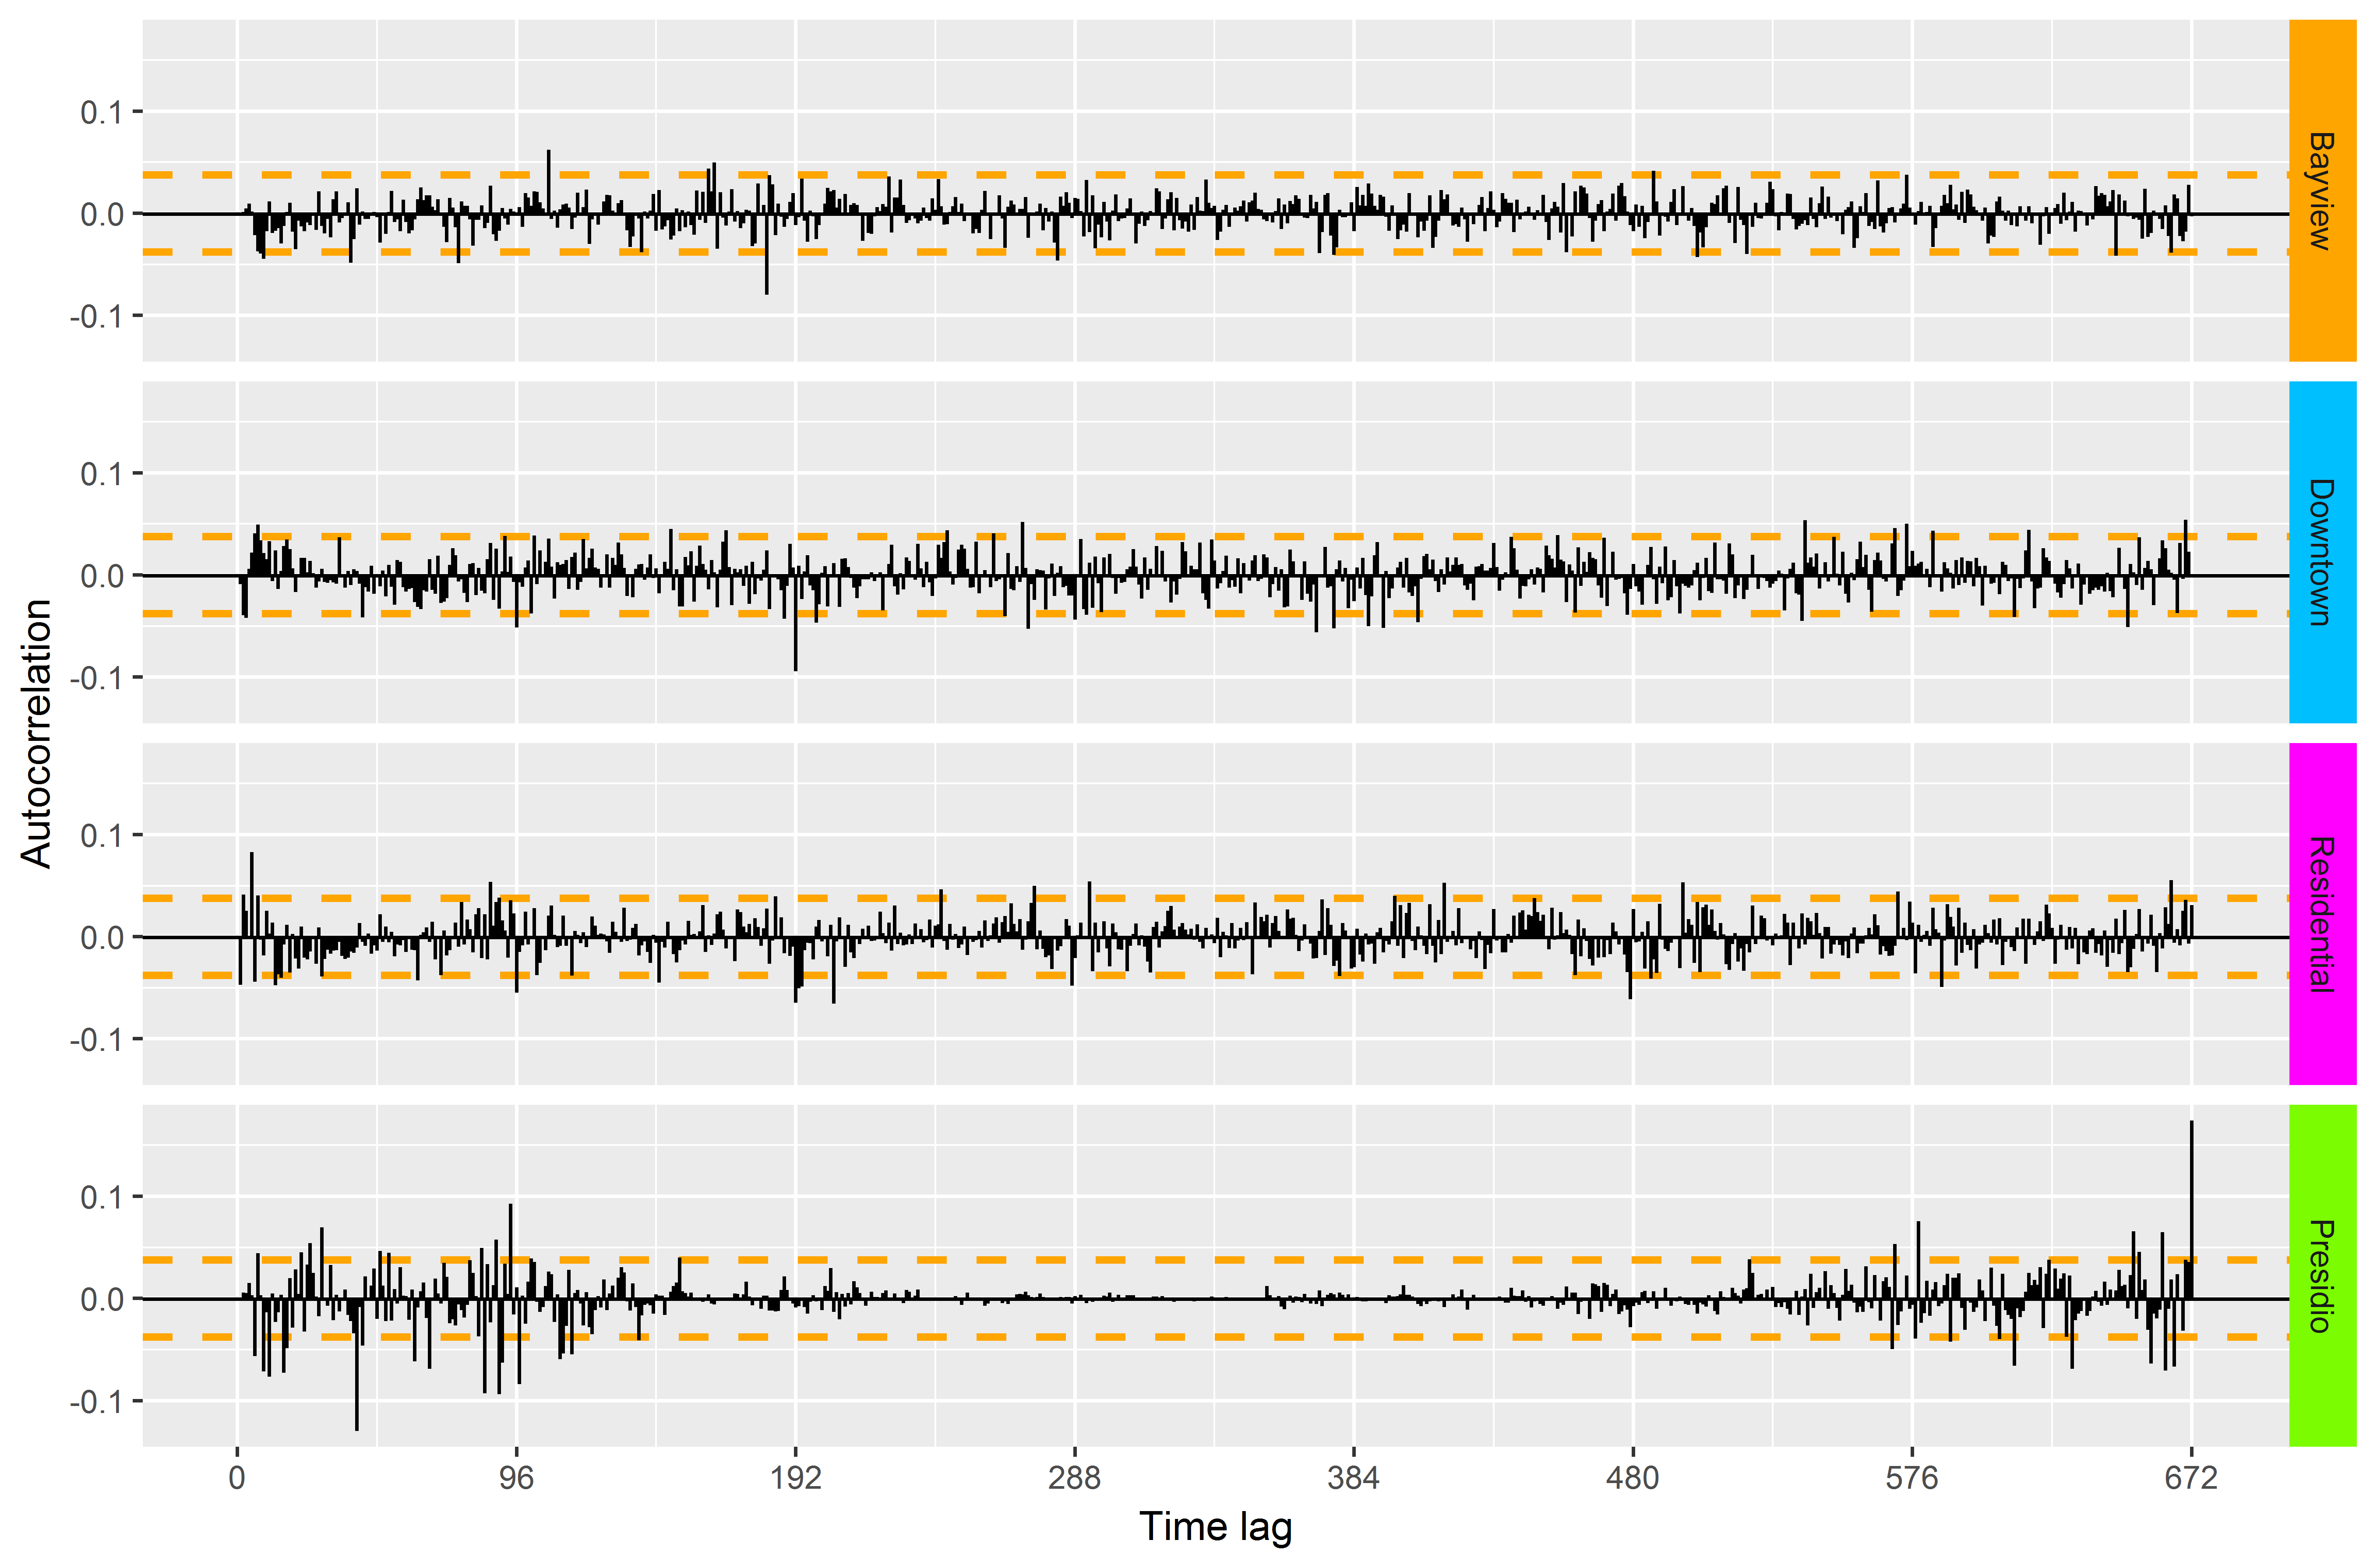
\includegraphics[width=\textwidth]{Figures/residual_acfplots} \caption{ACF plot of the model residuals}\label{fig:residualacf}
\end{figure}
Finally, Figure 5.7 shows the histograms of the model residual
distributions. As expected, for the Bayview and Presidio models, most
values are clustered closely around the zero mean, with the tails being
extremely thin and long, especially for the Bayview model. The residuals
of the Downtown and Residential models follow a distribution that comes
closer to a normal one, but also here, the tails are wide.
\begin{figure}[H]
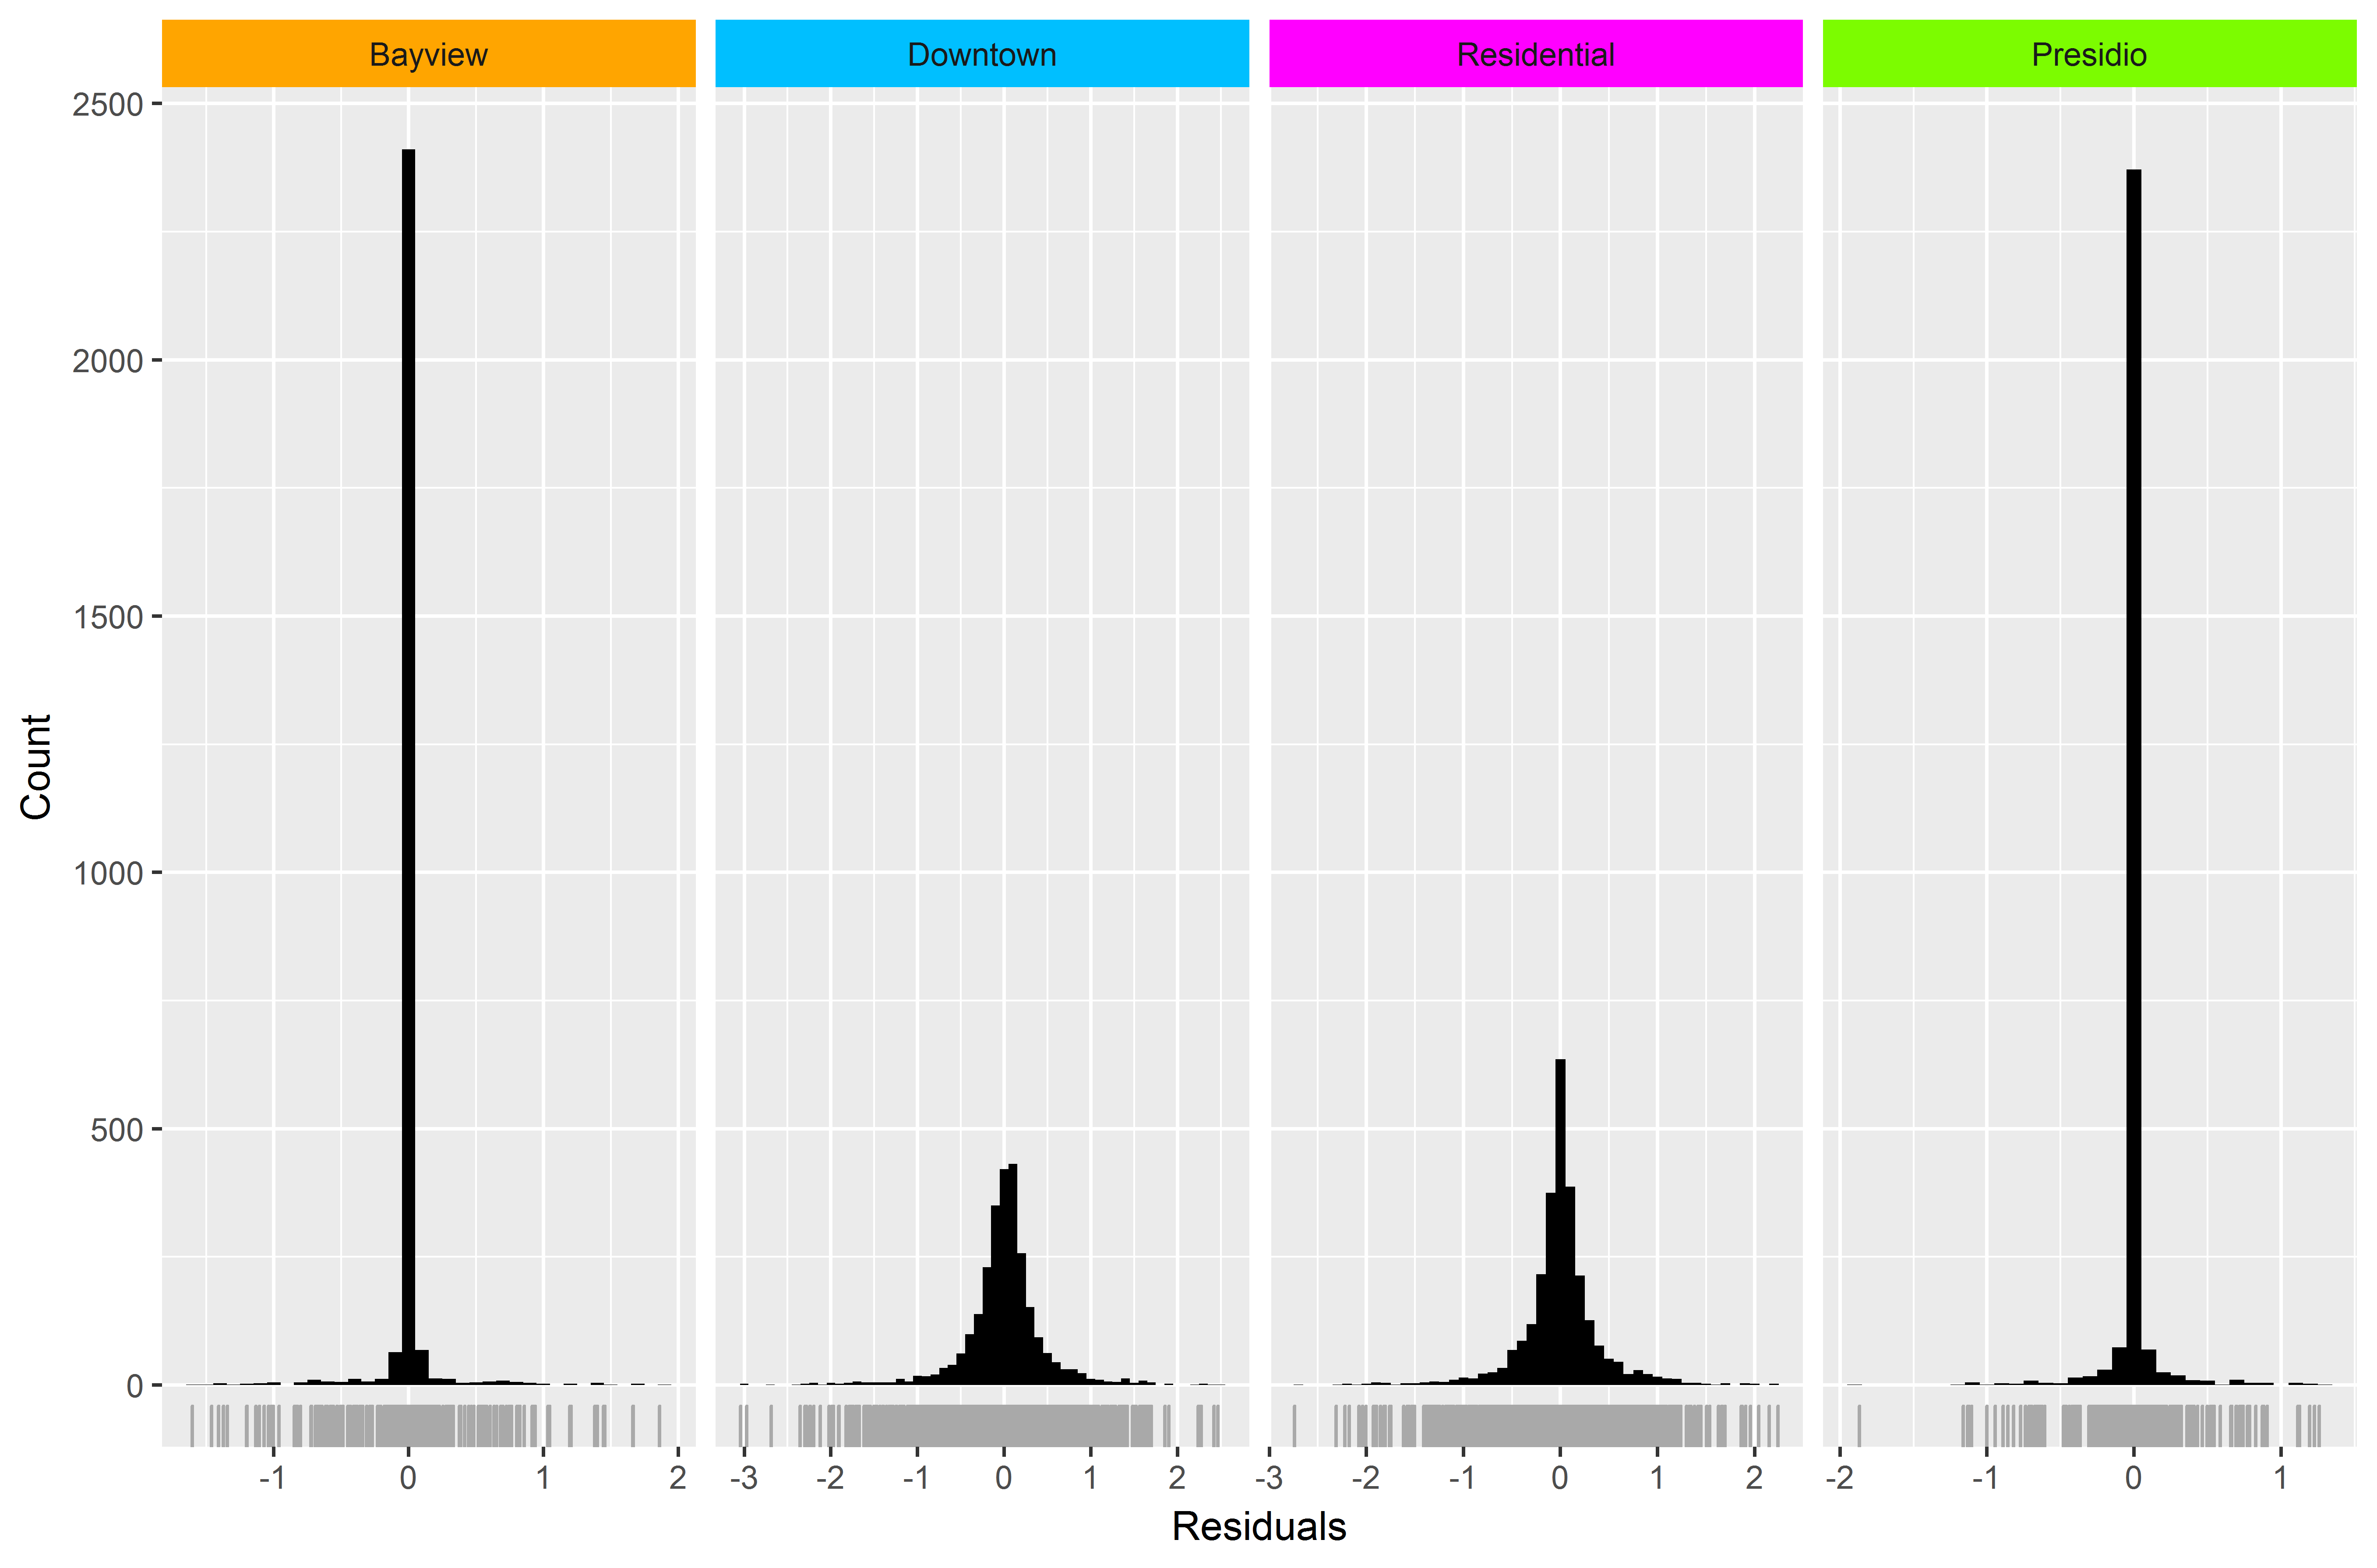
\includegraphics[width=\textwidth]{Figures/residual_histograms} \caption{Histograms of the model residuals}\label{fig:residualhist}
\end{figure}
\section{Forecasting}\label{forecasting-1}

Figure 5.8a shows the spatial distribution of the 500 test points. As
planned, areas with high usage intensity have more test points, with
94\% located in the Downtown and Residential clusters,and only the
minimum of ten test points in the Bayview cluster. Figure 5.8b shows the
temporal distribution test points. All days in the test week are well
covered, with less test points during working times and in the night,
and more during the morning rush hours and in the evening. On weekend
days, there is only one strong peak, around noon. Furthermore, it can be
seen that the morning peak on November 1st is somewhat lower compared to
the other weekdays. This may be, because it is the morning of All
Saint's Day, following the Halloween night. For the full information on
the test points, with all unique location-time combinations, see
Appendix A.
\begin{figure}[H]
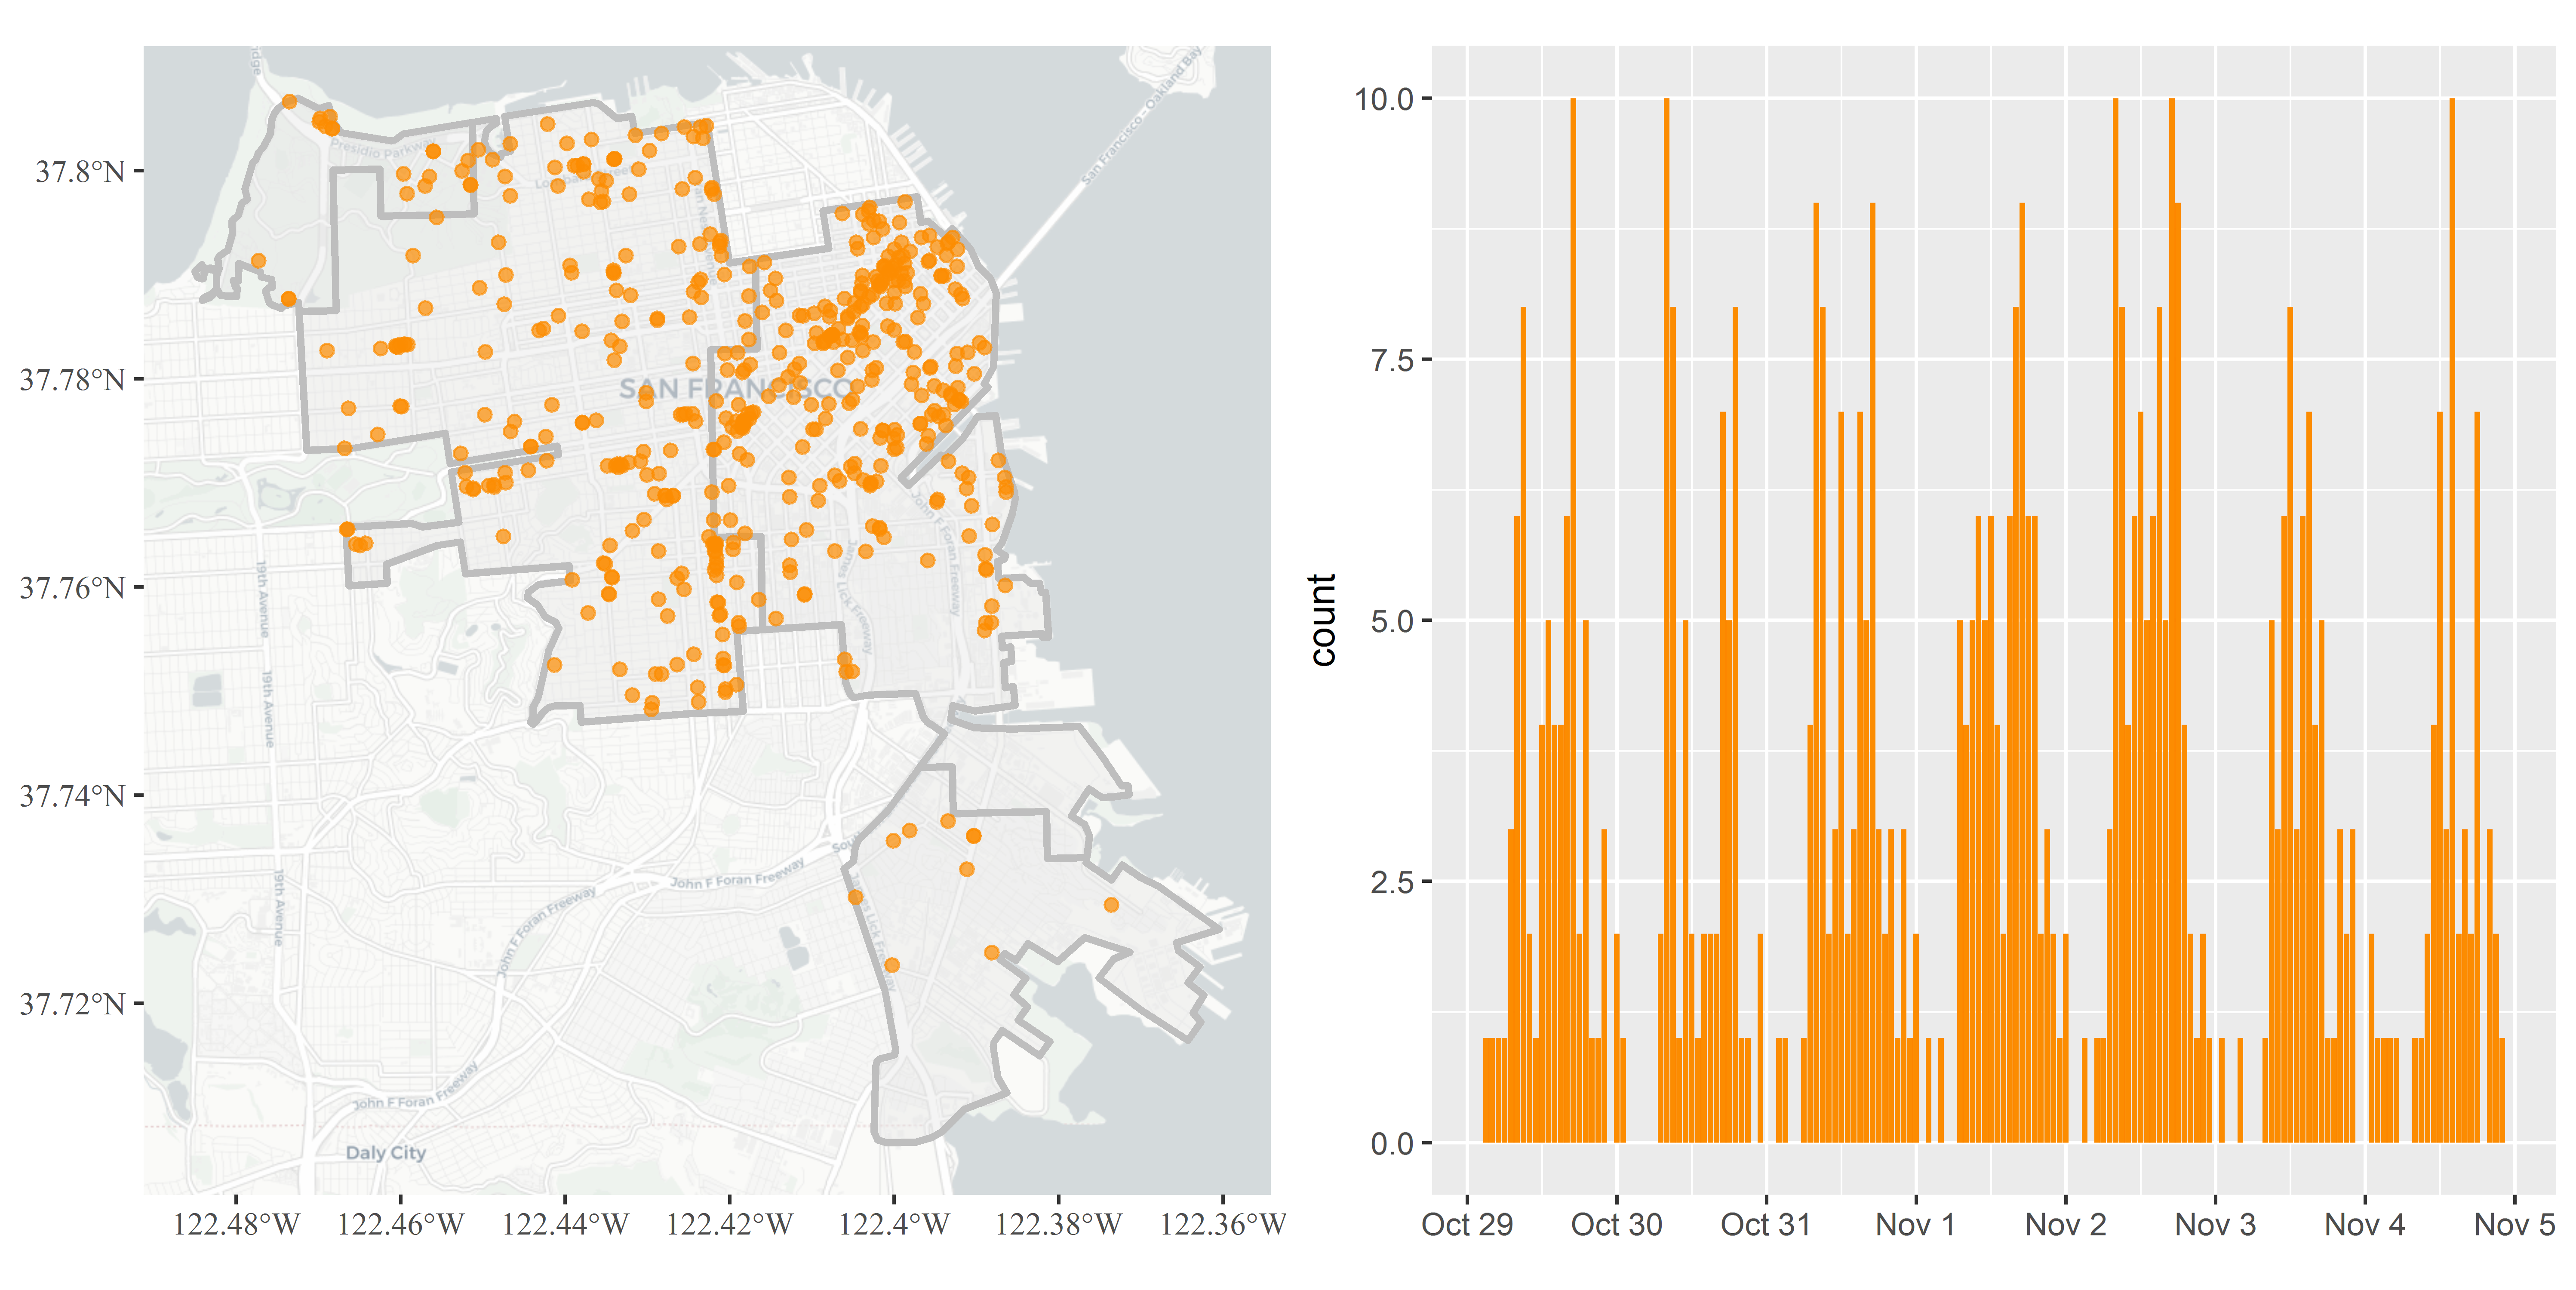
\includegraphics[width=\textwidth]{Figures/testpoints} \caption{a) test points locations; b) test point timestamps, counted per hour}\label{fig:testpoints}
\end{figure}
The first row of Table 5.3 lists the RMSE's, averaged over the whole
system area, of the forecasts produced by DBAFS, and of the forecasts
produced by the baseline system, NFS. DBAFS clearly outperforms NFS, by
producing forecasts with errors that are on average 31\% lower.
Furthermore, the range of error values is much lower for DBAFS, than for
NFS. The minima are comparable, but NFS produces forecasts with error
values up to 1644 meters, while DBAFS never exceeds 1004 meters.
\begin{table}[H]

\caption{\label{tab:forecastresults}Forecast RMSE's, in meters}
\centering
\begin{tabular}{>{\bfseries\raggedright\arraybackslash}p{2cm}>{\raggedleft\arraybackslash}p{1.5cm}>{\raggedleft\arraybackslash}p{1.5cm}>{\raggedleft\arraybackslash}p{1.5cm}>{\raggedleft\arraybackslash}p{1.5cm}>{\raggedleft\arraybackslash}p{1.5cm}>{\raggedleft\arraybackslash}p{1.5cm}r}
\toprule
\multicolumn{2}{c}{ } & \multicolumn{3}{c}{DBAFS} & \multicolumn{3}{c}{NFS} \\
\cmidrule(l{3pt}r{3pt}){3-5} \cmidrule(l{3pt}r{3pt}){6-8}
  & n & mean & min & max & mean & min & max\\
\midrule
\rowcolor{gray!6}  Total & 500 & 282 & 38 & 1004 & 408 & 37 & 1644\\
Bayview & 10 & 389 & 38 & 1004 & 389 & 38 & 1004\\
\rowcolor{gray!6}  Downtown & 259 & 248 & 122 & 523 & 414 & 116 & 927\\
Residential & 211 & 317 & 97 & 705 & 411 & 37 & 1644\\
\rowcolor{gray!6}  Presidio & 20 & 299 & 80 & 577 & 320 & 175 & 699\\
\bottomrule
\end{tabular}
\end{table}
Regarding the spatial patterns of the forecast errors, the remaining
rows of Table 5.3 show the RMSE's averaged per spatial cluster. With
NFS, the lowest errors are obtained in the Bayview and Presidio
clusters, where the data are less dynamic. In the Bayview cluster, NFS
gives the same results as DBAFS, and in the Presidio cluster, DBAFS
performs only slightly better than NFS. For DBAFS, however, the lowest
errors are not found in those clusters, but in the highly dynamic
Downtown cluster. Here, DBAFS gives errors that are 40\% lower than
those of NFS. In the Residential cluster, there are larger errors than
in the Downtown cluster, but also here, DBAFS outperforms NFS with
errors that are 23\% lower. It shows the strength of DBAFS in
forecasting dynamic data, when compared to NFS.

Regarding the temporal patterns of the forecast errors, Figure 5.10
shows the RMSE's averaged per hour of the day, and per forecast lag. The
lowest forecast errors occur during the night, when the usage intensity
of the system is low. During the day, higher errors occur, with peaks at
the morning peak hour, around noon (i.e.~the peak hour in the weekend)
and after working hours. This patterns are similar for NFS, but with
higher RMSE's at each hour. The forecast errors of both methods rise
steeply directly after the first forecast lag, but for NFS, this
increase is much larger than for DBAFS.

What strikes, is that the RMSE does not increase constantly when the
forecast horizon gets larger. From the forecasting lag of 12 hours, the
errors for both DBAFS and NFS decrease again. Moreover, at a forecasting
lag of approximately 18 hours, the RMSE of the DBAFS forecasts is, on
average, back at almost the same level as the one at a forecasting lag
of just 15 minutes. This conspicuousness can be explained as follows.
Most of the simulated forecast requests are made at times with a high
usage intensity, that are hard to forecast. The first forecast lags,
will still correspond to high usage times, but after a while, forecasts
will be made during night time. As could be seen in Figure 5.10a, these
night time forecasts have much lower errors. Therefore, it can happen
that, despite the length of the forecasting window, `far-ahead'
forecasts have lower errors than `close-by' forecasts.
\begin{figure}[h]
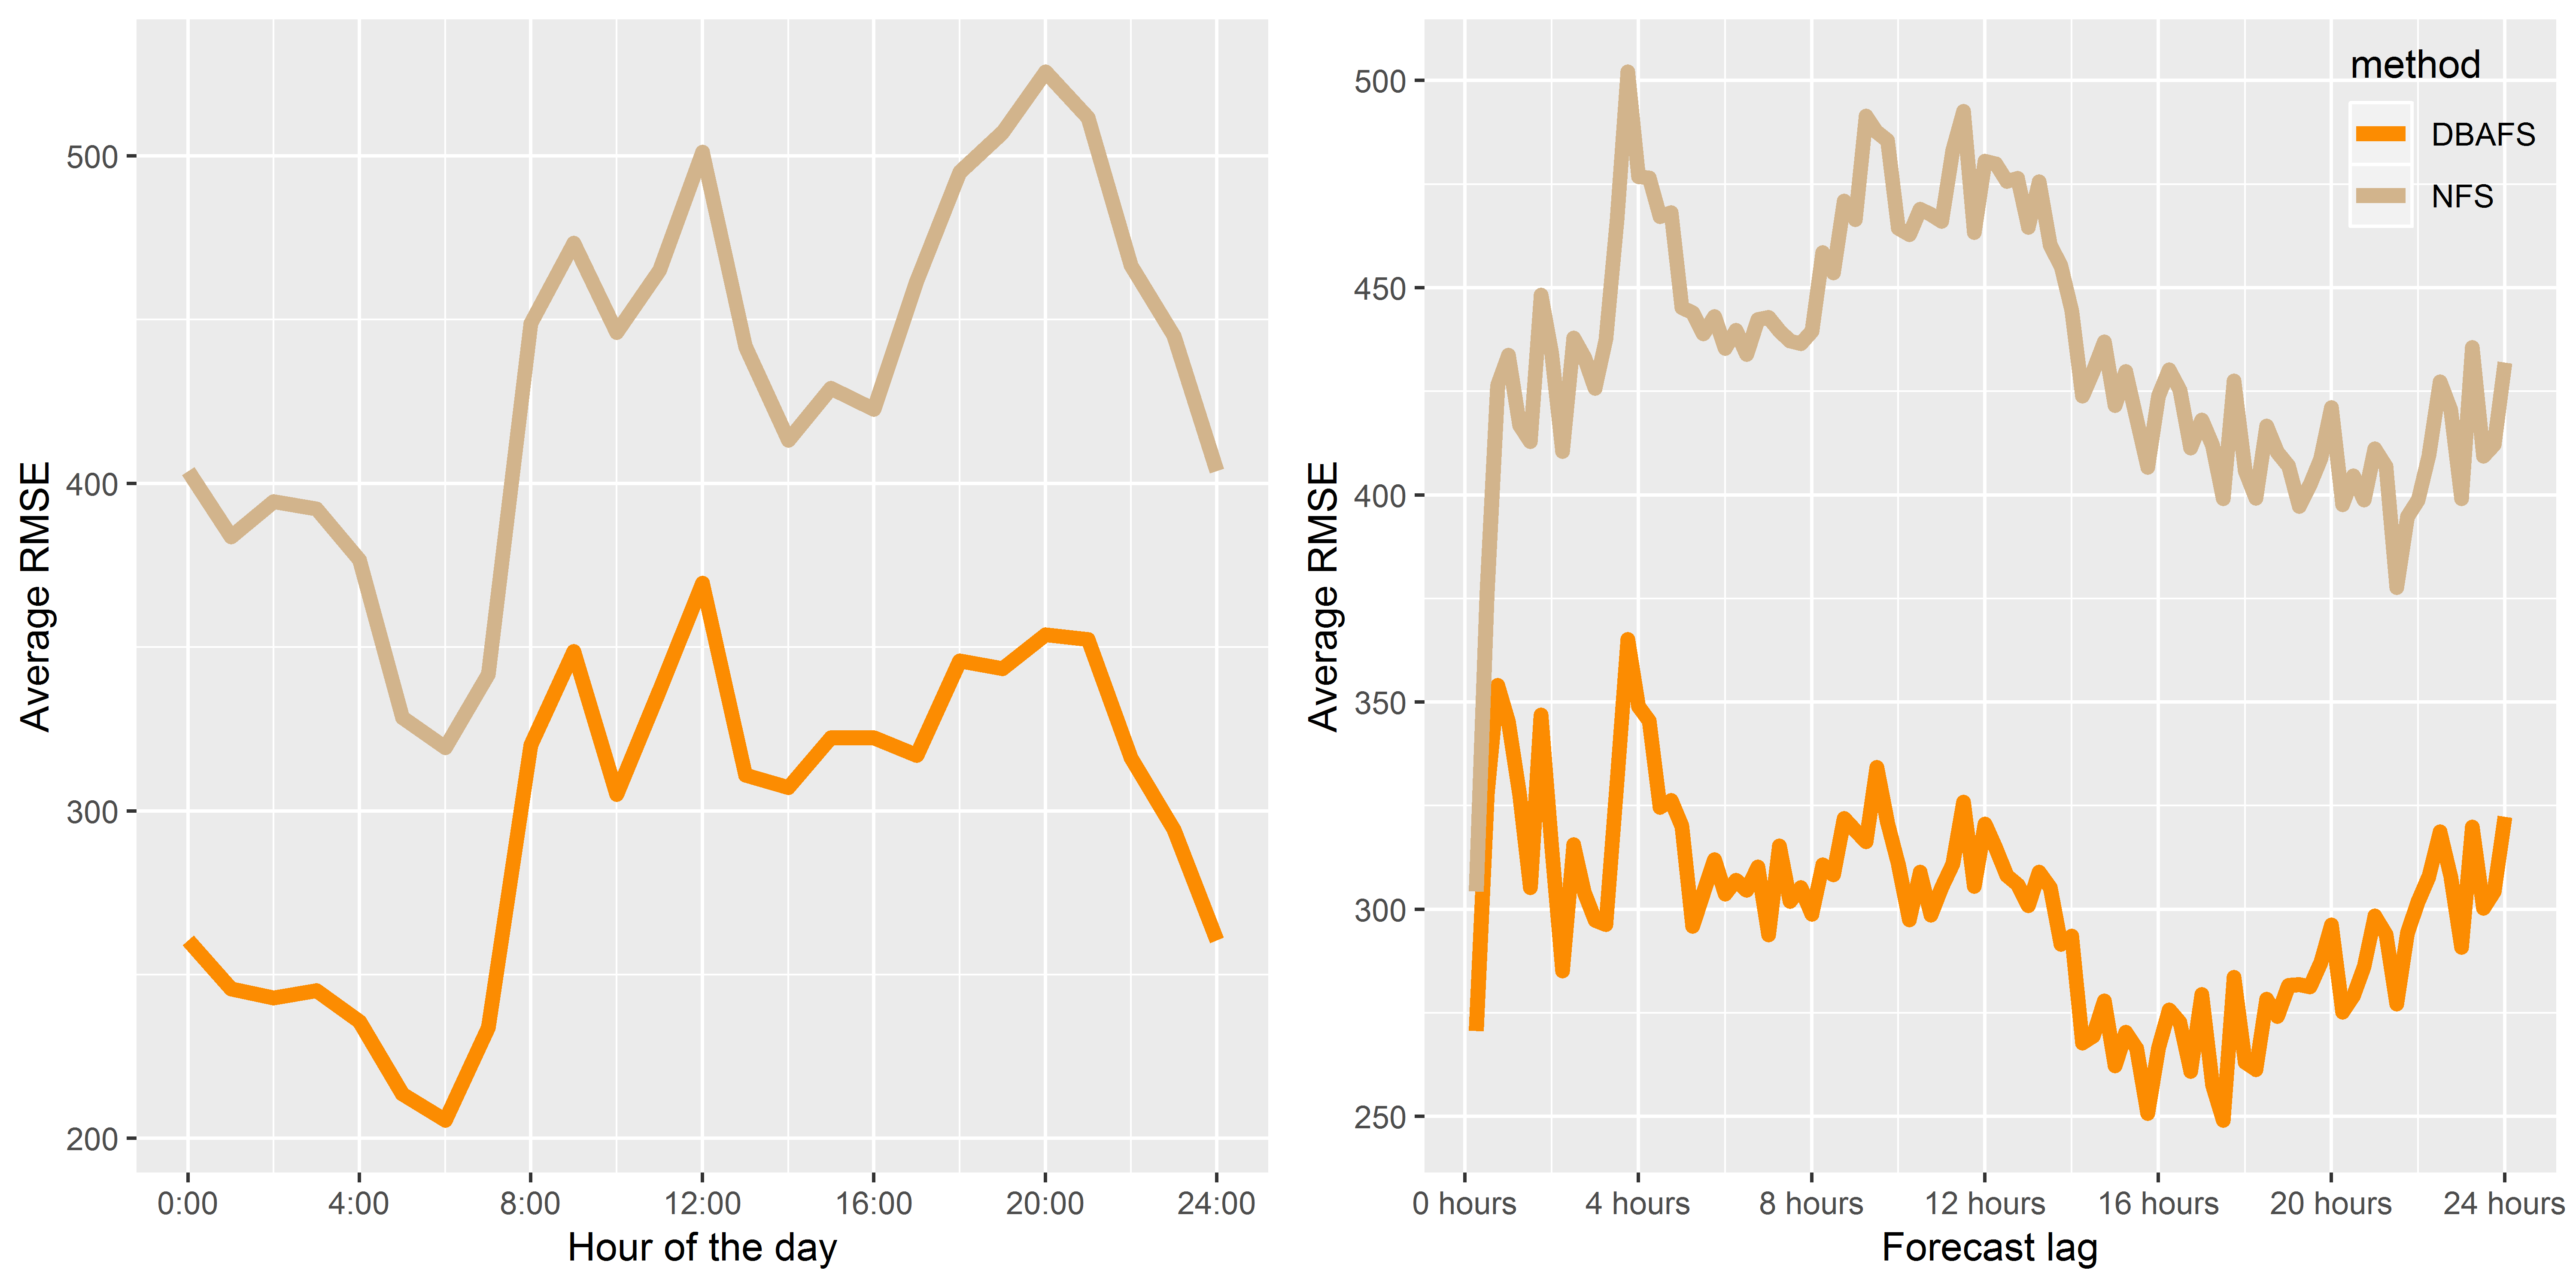
\includegraphics[width=\textwidth]{Figures/hourlag} \caption{a) RMSE averaged per hour of the day; b) RMSE averaged per forecast lag}\label{fig:timeandlag}
\end{figure}
\section{Limitations and
recommendations}\label{limitations-and-recommendations}

\subsection{Limits of forecastability}\label{limits-of-forecastability}

Although DBAFS outperforms the baseline, the average forecast RMSE of
almost 300 meters can be considered high when looking at it from an
absolute perspective. To get a more detailed understanding of the
performance of DBAFS, it may be benefitial to look at some individual
forecast results, rather than at general, averaged metrics. Therefore,
Figure 5.11 shows the forecasts at the four model point locations, for
the whole test period. Each day is forecasted seperately, with two weeks
of historical data.

As already pointed out earlier in this chapter, the forecasts in the
Bayview cluster act in a similar way as naïve forecasts, with straight
lines every day. Peaks in the true data occur randomly, and can not be
captured well by the fitted model. In the Downtown and Residential
clusters, the ones of primary interest, DBAFS performs very well in
forecasting when peaks are going to occur, but fails to accurately
capture the variation in the height of these peaks from day to day.
Equivalently, in the Presidio cluster, the varying amplitude of the
Sunday afternoon peak, is problematic for the forecasts. When this peak
has been relatively low in the two weeks before, DBAFS will expect it to
stay low, and never forecast the reoccurence of a higer peak.
\begin{figure}[H]
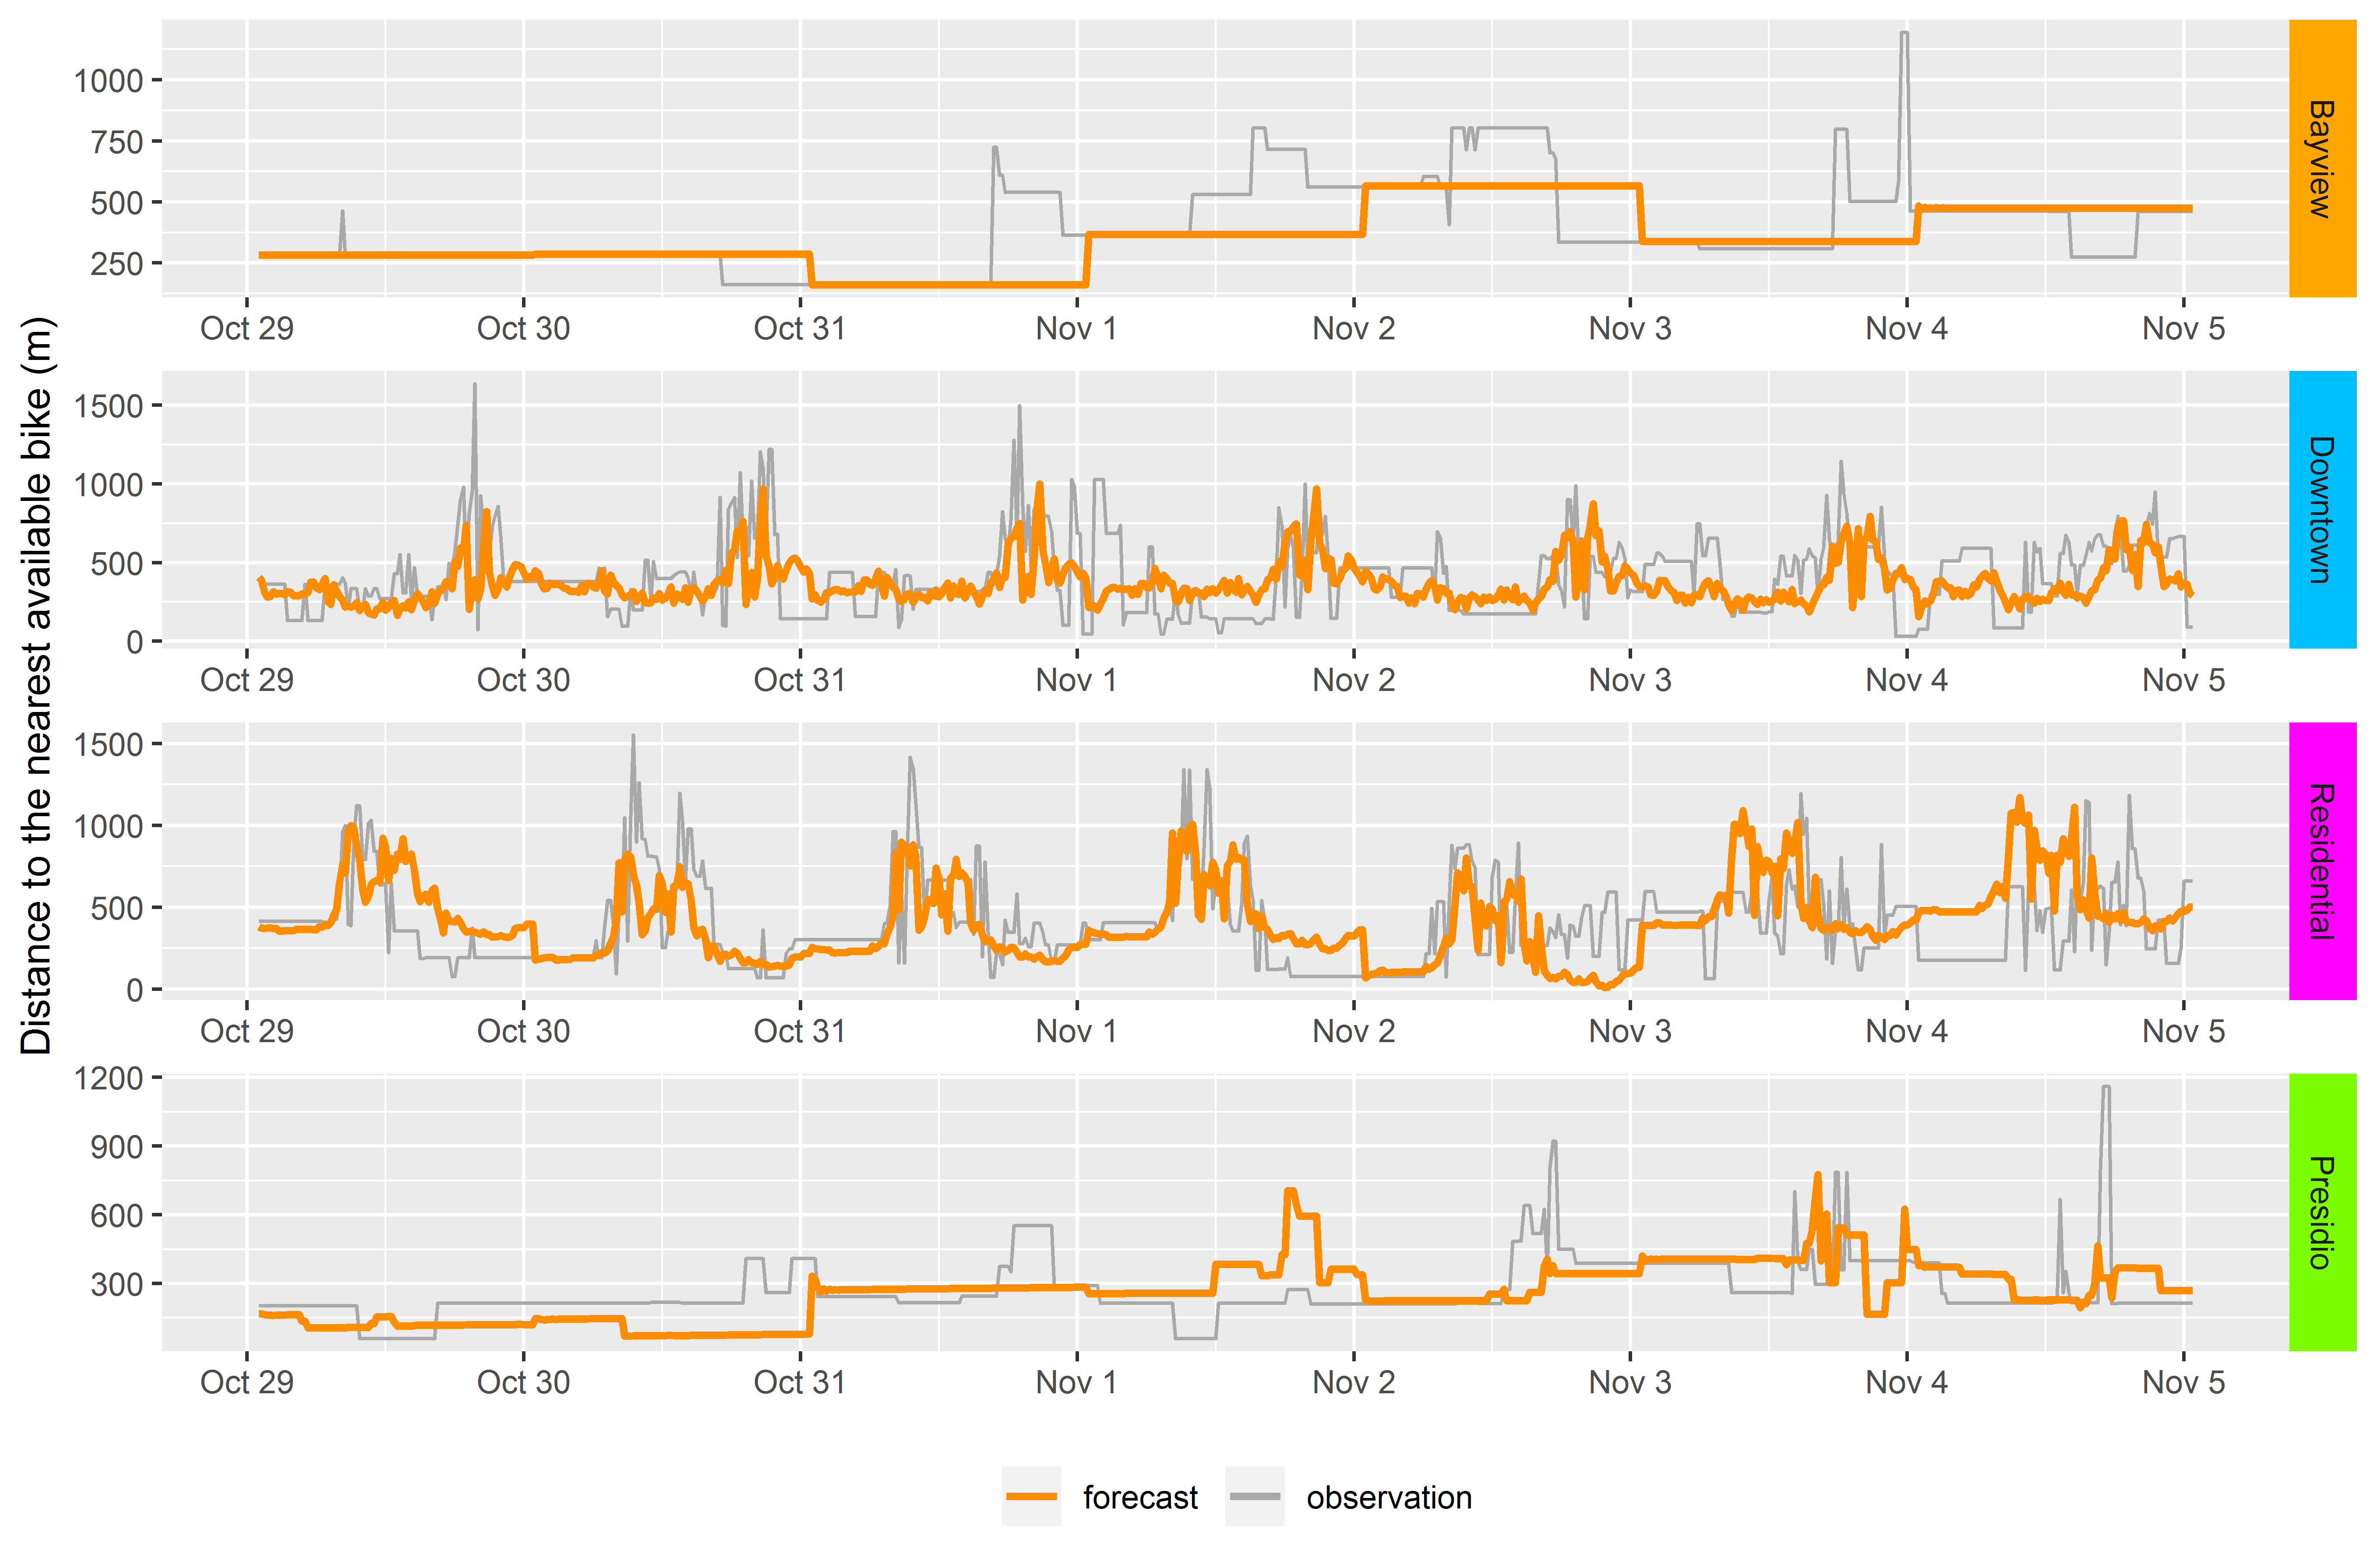
\includegraphics[width=\textwidth]{Figures/forecastplot} \caption{Detailed forecasts for the model point locations}\label{fig:forecastplot}
\end{figure}
The irregularity of the patterns in the data, and consequently, their
high entropy, can be linked to the flexible and dynamic nature of
dockless PBSS. Users can pick up bikes spontaneously, whenever they see
one around. This in contradiction to station-based PBSS, which have a
more organized structure, where trips are usually planned in advance, at
regular moments in time. Some studies in the United States already
explored these differences between dockless and station-based systems. A
report of the National Association of City Transportation Officials
showed that the usage in station-based systems follows typical commuting
patterns, while in dockless systems, it is more dispersed (NACTO,
\protect\hyperlink{ref-nacto2018}{2018}). This is in line with the
conclusions drawn from Figure 5.4, earlier in this chapter. Moreover,
Mckenzie (\protect\hyperlink{ref-mckenzie2018}{2018}) found similar
results in Washington DC.

In San Francisco, the differences between station-based and dockless
systems may even be stronger, for the following reason. For
single-trips, JUMP Bikes is cheaper than the station-based Ford GoBike
system. However, in contradiction to GoBike, JUMP Bikes has no
subscription pricing. That is, for irregular usage, JUMP Bikes is the
better option, but when using a JUMP Bike every working day for two
trips of half an hour (\$2 each), this will cost around \$1040 per year,
compared to only \$149 for a yearly subscription on GoBike (Harris,
\protect\hyperlink{ref-harris2018}{2018}).

To strenghten the findings discussed above, Figure 5.12 is adapted from
the mid-point evaluation of JUMP Bikes in San Francisco, performed by
SFMTA, and shows the number of trips per bike per day, for both JUMP
Bikes and GoBike, during five months in 2018 (SFMTA Board of Directors,
\protect\hyperlink{ref-sfmta2018three}{2018}). It clearly confirms the
expected differences between the two. The course of the GoBike line is
very regular, with peaks during weekdays, and valleys during weekends.
JUMP Bikes, in contradiction, follows a highly irregular pattern. Such
irregularity, obviously, sets limits on the ability of models to
forecast the data accurately.

\subsection{Exogeneous variables}\label{exogeneous-variables}

That the forecastability of dockless bike sharing data is limited, does
not mean that the forecasts produced by DBAFS can not be improved in any
way. There may be exogeneous variables that can explain at least a part
of the variation in peak height from day to day. The most relevant of
those, probably relate to weather conditions. Several studies addressed
the relationship between cycling activity in PBSS and weather conditions
already (Campbell, Cherry, Ryerson, \& Yang,
\protect\hyperlink{ref-campbell2016}{2016}; Corcoran, Li, Rohde,
Charles-Edwards, \& Mateo-Babiano,
\protect\hyperlink{ref-corcoran2014}{2014}; Faghih-Imani, Eluru,
El-Geneidy, Rabbat, \& Haq, \protect\hyperlink{ref-faghih2014}{2014};
Shen et al., \protect\hyperlink{ref-shen2018}{2018}). Most notably,
heavy rain or snowfall, high humidity, strong winds, extremely low
temperatures, and extremely high temperatures, all have a negative
impact on PBSS usage, both for recreational and commuting trips. It must
be noted, that DBAFS already deals with long-term weather variations,
since models are updated regularly, and moreover, STL allows the
seasonal pattern to change slightly over time. The short-term weather
variation, however, may be an important factor influencing the
variability in the data, which DBAFS is not able to account for.
Therefore, including weather condition variables in the forecasting
system, can possibly decrease the forecast errors substantially.
\begin{figure}[H]
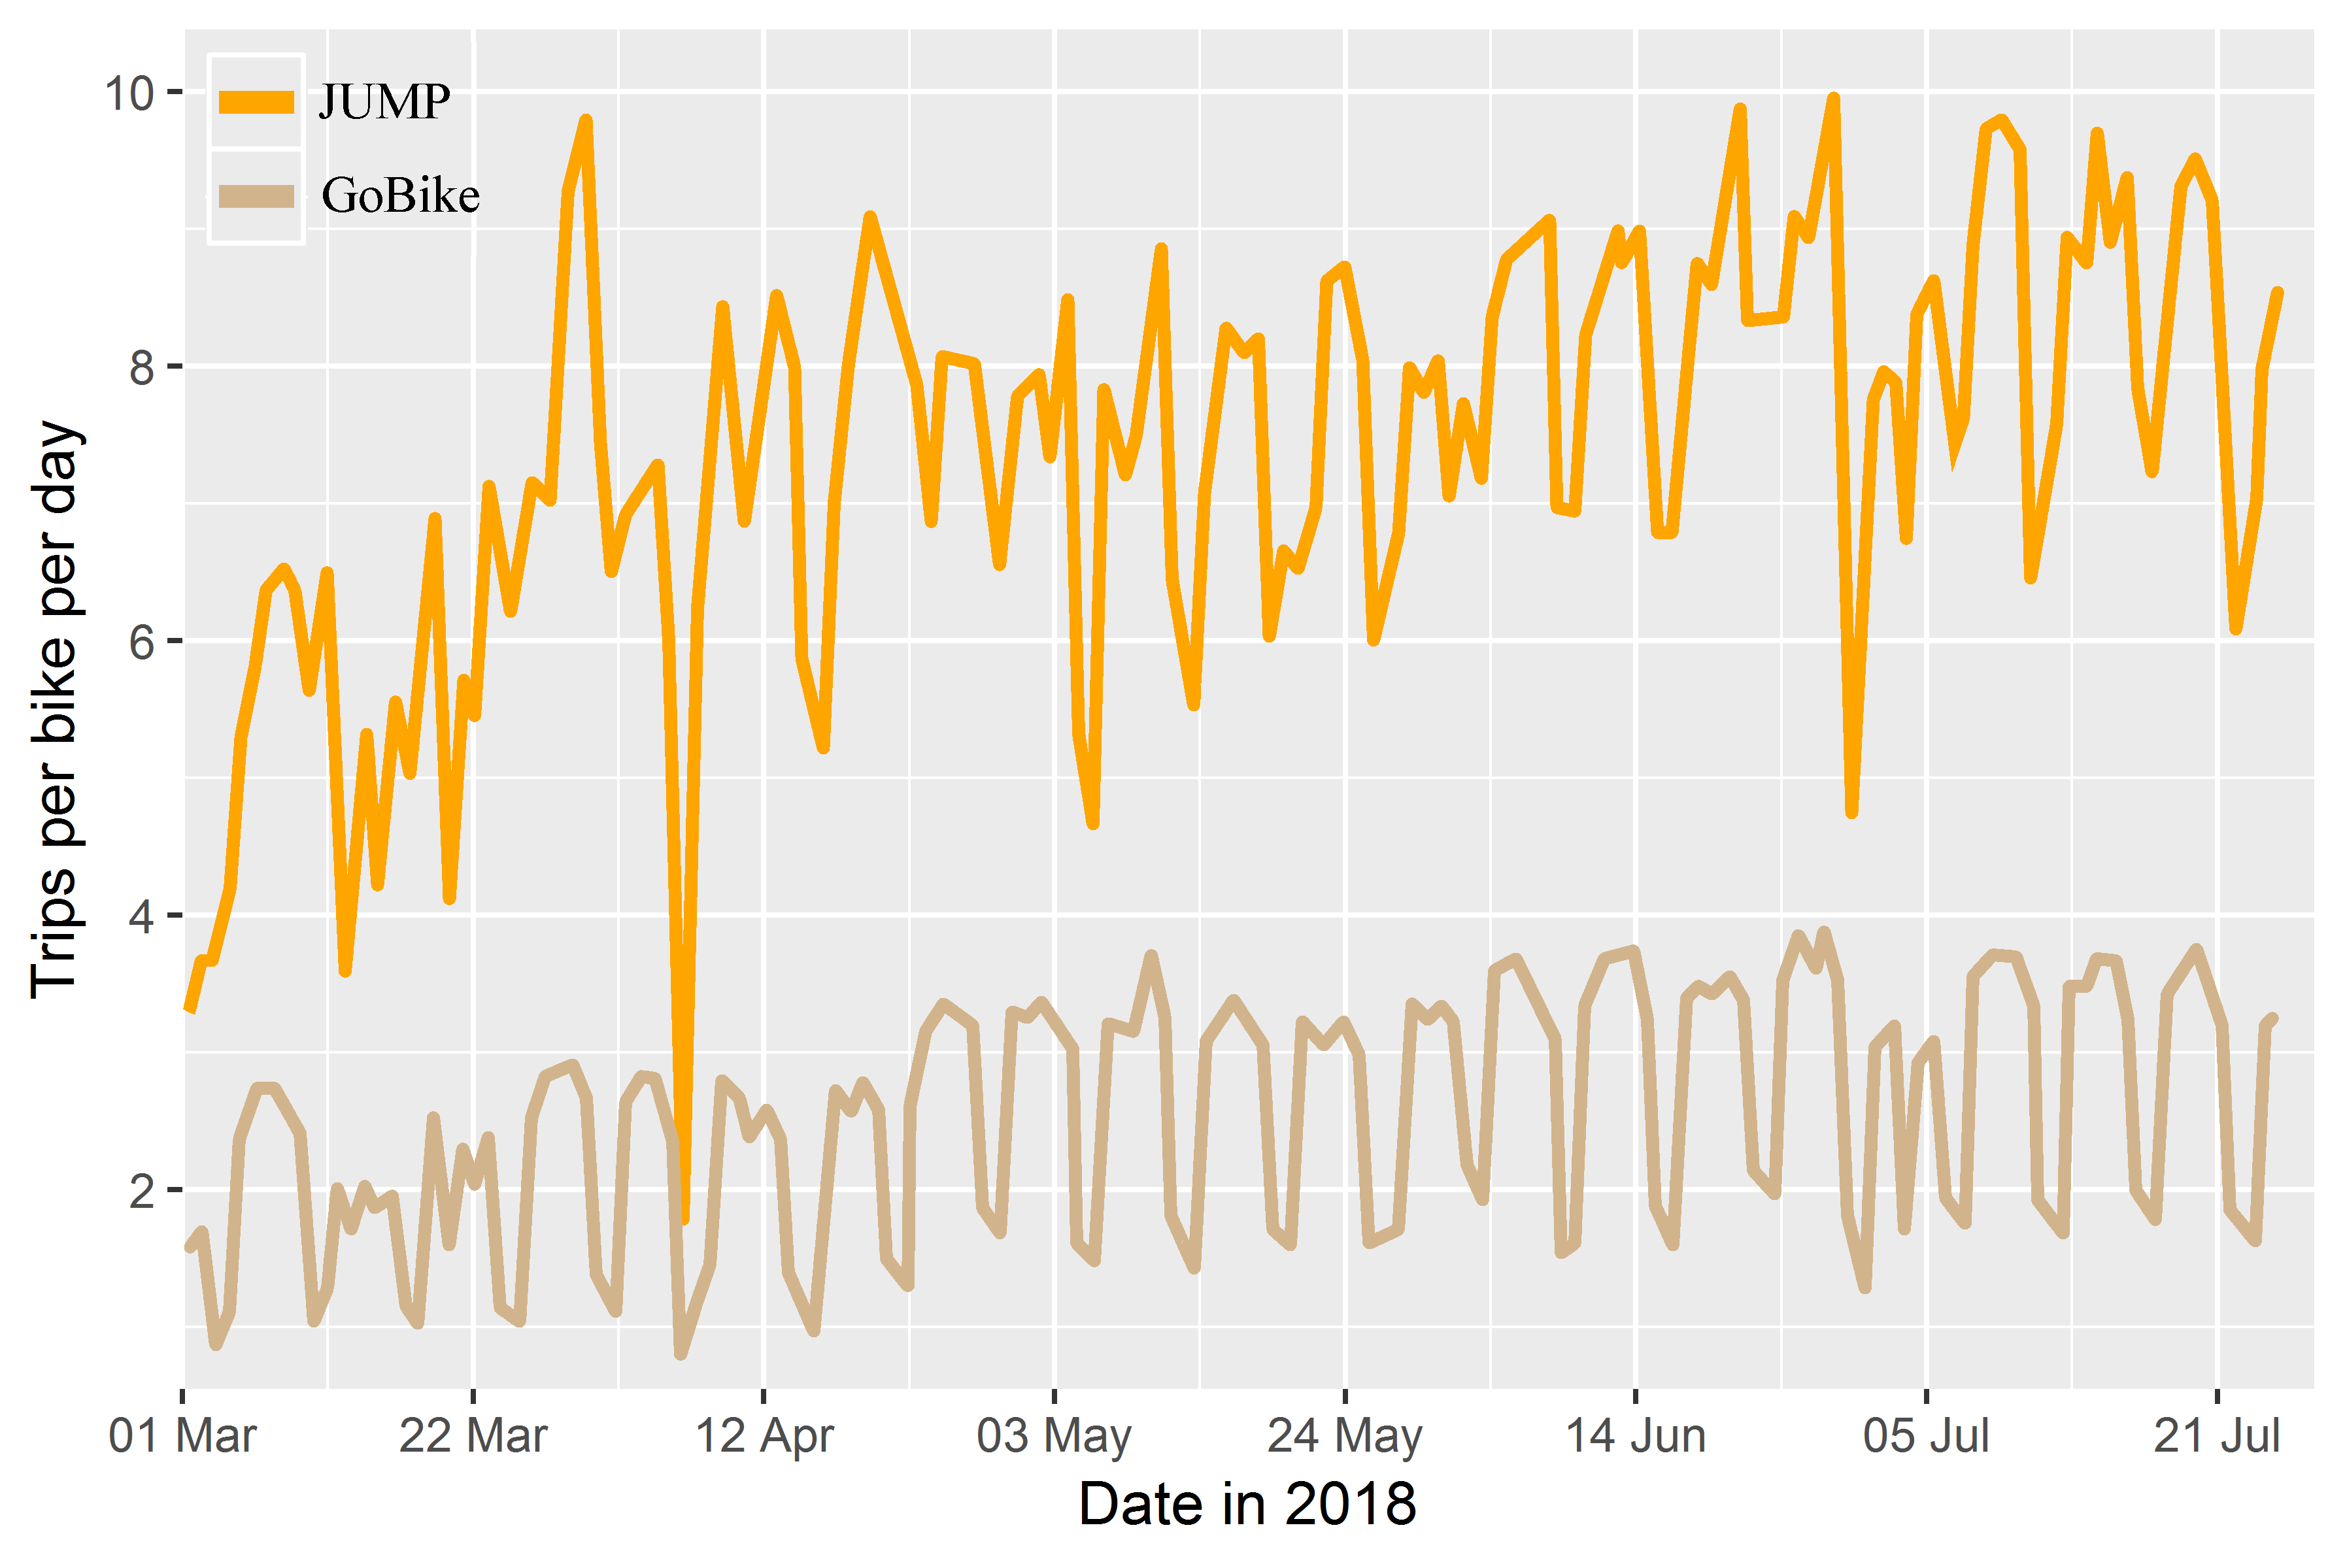
\includegraphics[width=\textwidth]{Figures/jumpgo} \caption{Dockless versus station-based, adapted from SFMTA}\label{fig:jumpgo}
\end{figure}
Above average peaks in the data may occur when special events, such as
sport matches, concerts or conferences, take place. Furthermore, public
holidays may cause abnormal data patterns (Corcoran et al.,
\protect\hyperlink{ref-corcoran2014}{2014}). These are also factors that
are not considered by DBAFS. Modelling their relationship with PBSS
usage is complicated, especially for the events, since the influence
will not be the same at all locations within each cluster. However, they
will contain information that can explain a part of the variability in
the data, as well.

As explained in section 2.4.1, time series forecasting models relate
future patterns to past patterns in the same data. That is, in essence,
they do not allow for exogeneous variables. However, several methods
have been developed to overcome this issue. For example, Hyndman \&
Athanasopoulos (\protect\hyperlink{ref-hyndman2018fpp}{2018}) recommend
dynamic regression models, in which the exogeneous variables are
included in a linear regression, with an ARIMA(\(p\), \(d\), \(q\))
model fitted to the autocorrelated errors. Optionially, seasonal
patterns can be captured by including Fourier terms in the regression as
well. Another option is the \texttt{fasster} package in R (O'Hara-Wild,
\protect\hyperlink{ref-fasster}{2018}), which is, at the time of
writing, still under development. Fasster stands for `Forecasting with
Additive Switching of Seasonality, Trend and Exogenous Regressors', and
is a model is designed to capture both the influence of exogeneous
regressors as multiple seasonal patterns in a state space framework, by
using state switching. Finally, machine learning regression methods are
widely used in forecasting, and allow the use of exogeneous variables as
well. It is recommended to test these approaches with the exogeneous
variables described above, and examine the accuracy gain compared to the
current approach of DBAFS.

\subsection{Residual distributions and prediction
intervals}\label{residual-distributions-and-prediction-intervals}

Another point of concern regards the non-normality of the models'
residual distributions, which showed clearly in Figure 5.8. Both in the
calculation of the AIC, for model selection, and in the estimation of
the model parameters, Gaussian likelihood is used, assuming a normal
distribution. In the literature, approaches have been developed to use
different likelihood functions, such as the Laplace Likelihood and
Student's t likelihood, that may be more appropriate to use for models
with widely tailed residual distributions such as those identified in
Figure 5.8 (Huang \& Pawitan, \protect\hyperlink{ref-huang2000}{2000};
Lehr \& Lii, \protect\hyperlink{ref-lehr1998}{1998}; W. K. Li \& McLeod,
\protect\hyperlink{ref-li1988}{1988}). However, such approaches will
increase the complexity of the system. Moreover, the accuracy gain will
probably be of minor extent, since, as discussed in section 2.4.2.4,
using Gaussian likelihood is sensible even for models with non-normally
distributed residuals, especially when sample sizes are large. It should
also be noted that in the \texttt{forecast} package, Gaussian likelihood
is the only available option.

The non-normality of the residuals does have an important effect on the
validity of the prediction intervals, however. When 95\% prediction
intervals are calculated, assuming normality of the forecast
distribution, they can not be interpreted as such. To emphasize this,
Table 5.4 shows the percentage of true observations that fall within the
calculated 95\% prediction interval of the forecasts. As can be seen,
for all clusters, and especially those where seasonality was detected,
this percentage is extremely low. That is, the calculated prediction
intervals are far to narrow, making them not useful in any sense.
\begin{table}[H]

\caption{\label{tab:intervalcheck}Interpretation of the calculated prediction intervals}
\centering
\begin{tabular}{>{\bfseries\raggedright\arraybackslash}p{4cm}r}
\toprule
  & Percentage of observations within 95\% prediction interval\\
\midrule
\rowcolor{gray!6}  Total & 0.9\\
Bayview & 17.5\\
\rowcolor{gray!6}  Downtown & 0.5\\
Residential & 0.6\\
\rowcolor{gray!6}  Presidio & 0.1\\
\bottomrule
\end{tabular}
\end{table}
As proposed by Hyndman \& Athanasopoulos
(\protect\hyperlink{ref-hyndman2018fpp}{2018}), in the case of
non-normally distrubuted model residuals, a technique called
bootstrapping is a useful alternative for calculating prediction
intervals. It does not make assumptions about the distribution of the
residuals, and only requires them to be uncorrelated. Many possible
futures for each forecasted time lag are obtained by repeatingly
sampling from the model residuals, and replacing the error terms of the
forecasts (see Equation 2.x) by these sampled values. Then, the 95\%
prediction interval for each forecast is equal to the interval that
contains 95\% of the calculated `possible futures'. A detailed
description of this technique is given in McCullough
(\protect\hyperlink{ref-mccullough1994}{1994}).

Another important reason for the extremely narrow prediction intervals,
is that not all sources of uncertainty are included in its calculation.
In DBAFS, there are at least six different sources of uncertainty.
\begin{itemize}
\tightlist
\item
  The random error component of the ARIMA(\(p\), \(d\), \(q\)) model.
\item
  The parameter estimates of the ARIMA(\(p\), \(d\), \(q\)) model.
\item
  The choice of the model.
\item
  The continuation of the data generating process into the future.
\item
  The continuation of the seasonal patterns into future.
\item
  The use of a model fitted on the model point's data, for other
  locations within the same cluster.
\end{itemize}
In the \texttt{forecast} package, only the first of these sources is
taken into account when calculating prediction intervals (Hyndman \&
Athanasopoulos, \protect\hyperlink{ref-hyndman2018fpp}{2018}). In most
cases, this leads to acceptable estimates. Even when an ARIMA forecast
is combined with a seasonal naïve forecast, this is often true, since
seasonal patterns are expected to be constant. However, as already
noticed earlier in this chapter, in dockless bike sharing data, there
may be a large variation from season to season, and simply ignoring the
seasonal uncertainty, is not valid anymore. Bootstrapping can help to
partly overcome this issue as well. However, that is a time consuming
process, and therefore not suitable to perform at every individual
forecast. That is, it still does not account for the last source of
uncertainty, which influence is expected to be large. Hence, to provide
sensible prediction intervals, an adequate methodology that captures all
sources of uncertainty to an acceptable extent, should be developed.

\subsection{GPS accuracy}\label{gps-accuracy}

\chapter{Conclusion}\label{conclusion}

This thesis presented a fully automated forecasting system for bike
availability in dockless bike sharing systems. To balance speed and
accuracy, the system took advantage of the spatio-temporal nature of the
data, and used an approach in which the structures of forecasting models
build at specific locations and specific timestamps, were inherited by
forecast requests for nearby locations, and future timestamps.

The proposed system was tested through a case study in San Francisco,
California. The results showed that time series forecasting models,
nested inside the proposed structure of model inheritance, can produce
forecasts that outperform simple baseline methods. However, they also
highlighted the limited forecastability of dockless bike sharing data,
especially when compared to conventional station-based systems.

In future studies that adress the same problem, the forecast accuracy
may be improved by incuding exogeneous variables, related to weather
conditions and special events, which can explain some of the uncaptured
variation. Furthermore, methodolgies to provide sensible prediction
intervals, need to be developed.

Results are believed to be of direct, practical interest for operators
of dockless bike sharing systems. In the broader picture, the most
important contribution of this thesis is that it is one of the first
works that aimed to get a deeper, scientific understanding of the
spatio-temporal dynamics of dockless bike sharing systems, and the
forecastability of their data. As such, it took a new step on the way to
reliable, convenient bike sharing systems, that can provide a serious
alternative to motorized transport, and increase the liveability in
urban environments.

\appendix

\chapter{Code}\label{code}
\begin{wrapfigure}{R}{.35\textwidth}  
 \begin{center}
    
\includegraphics[width=.3\textwidth]{Figures/hexagon.png}  
\end{center}
\end{wrapfigure}
All the R code used in this thesis, as well as the nested SQL code, is
bundled in the \texttt{dockless} package (Van der Meer,
\protect\hyperlink{ref-dockless}{2019}). Its source code, including
documentation for each function, can be found on GitHub, through the
following link: \url{https://github.com/luukvdmeer/dockless}. An R
version of at least 2.10 is required. The package is optimized for the
case study in San Francisco, but can easily be adapted to other systems.

The JUMP Bikes database is not openly accessible. Therefore, to query
the data, and pre-process them on the database server, database
credentials are needed. Please contact the author for more information.
However, to enable reproducibility, all necessary pre-processed datasets
have been included in the package. These are the following:
\begin{itemize}
\tightlist
\item
  \texttt{distancedata\_centroids}: an object of class
  \texttt{dockless\_dfc} containing the distance data for all 249 grid
  cell centroids, during the training period.
\item
  \texttt{distancedata\_modelpoints}: an object of class
  \texttt{dockless\_dfc} containing the distance data for all 4 model
  points, during the training period.
\item
  \texttt{distancedata\_testpoints}: an object of class
  \texttt{dockless\_dfc} containing the distance data for all 500 test
  points, during the test period, and the two weeks before.
\item
  \texttt{usagedata\_train}: an object of class \texttt{sf} with POINT
  geometry, containing all calculated pick-ups during the training
  period.
\item
  \texttt{usagedata\_test}: an object of class \texttt{sf} with POINT
  geometry, containing all calculated pick-ups during the test period.
\item
  \texttt{testpoints}: an object of class \texttt{sf} with POINT
  geometry, containing all location-timestamp combinations of the 500
  test points.
\item
  \texttt{systemarea}: an object of class \texttt{sf} with POLYGON
  geometry, containing the geographical outline of the JUMP Bikes system
  area in San Francisco.
\end{itemize}
The \texttt{dockless} package can be downloaded from github with the
following code. Please make sure that the \texttt{devtools} package is
installed in advance.\\
\begin{Shaded}
\begin{Highlighting}[]
\NormalTok{devtools}\OperatorTok{::}\KeywordTok{install_github}\NormalTok{(}\StringTok{'luukvdmeer/dockless'}\NormalTok{)}
\end{Highlighting}
\end{Shaded}
Then, the complete analysis can be reproduced as follows. Furthermore,
reproducible scripts for all tables and figures in chapter 5 can be
found through the following link:
\url{https://github.com/luukvdmeer/dockless/tree/master/scripts}\\
\begin{Shaded}
\begin{Highlighting}[]
\KeywordTok{require}\NormalTok{(dockless)}
\KeywordTok{require}\NormalTok{(sf)}

\NormalTok{## ----------------------- CLUSTER LOOP --------------------------}
\CommentTok{# Create grid}
\NormalTok{gridcells =}\StringTok{ }\NormalTok{dockless}\OperatorTok{::}\KeywordTok{create_grid}\NormalTok{(}
  \DataTypeTok{area =}\NormalTok{ systemarea,}
  \DataTypeTok{cellsize =} \KeywordTok{c}\NormalTok{(}\DecValTok{500}\NormalTok{, }\DecValTok{500}\NormalTok{)}
\NormalTok{)}

\CommentTok{# Calculate grid cell centroids}
\NormalTok{gridcentroids =}\StringTok{ }\NormalTok{gridcells }\OperatorTok
\StringTok{  }\NormalTok{dockless}\OperatorTok{::}\KeywordTok{project_sf}\NormalTok{() }\OperatorTok
\StringTok{  }\NormalTok{sf}\OperatorTok{::}\KeywordTok{st_centroid}\NormalTok{() }\OperatorTok
\StringTok{  }\NormalTok{sf}\OperatorTok{::}\KeywordTok{st_transform}\NormalTok{(}\DataTypeTok{crs =} \DecValTok{4326}\NormalTok{)}

\CommentTok{# Usage intensity per grid cell}
\NormalTok{gridcells}\OperatorTok{$}\NormalTok{intensity =}\StringTok{ }\NormalTok{dockless}\OperatorTok{::}\KeywordTok{usage_intensity}\NormalTok{(}
  \DataTypeTok{usage =}\NormalTok{ usagedata_train,}
  \DataTypeTok{grid =}\NormalTok{ gridcells}
\NormalTok{)}

\CommentTok{# Add intensity information to grid cell centroids}
\NormalTok{gridcentroids}\OperatorTok{$}\NormalTok{intensity =}\StringTok{ }\NormalTok{gridcells}\OperatorTok{$}\NormalTok{intensity}

\CommentTok{# Cluster}
\NormalTok{clusters =}\StringTok{ }\NormalTok{dockless}\OperatorTok{::}\KeywordTok{spatial_cluster}\NormalTok{(}
  \DataTypeTok{data =}\NormalTok{ distancedata_centroids,}
  \DataTypeTok{grid =}\NormalTok{ gridcells,}
  \DataTypeTok{area =}\NormalTok{ systemarea,}
  \DataTypeTok{K =} \KeywordTok{c}\NormalTok{(}\DecValTok{3}\OperatorTok{:}\DecValTok{10}\NormalTok{),}
  \DataTypeTok{omega =} \KeywordTok{seq}\NormalTok{(}\DecValTok{0}\NormalTok{, }\DecValTok{1}\NormalTok{, }\FloatTok{0.1}\NormalTok{)}
\NormalTok{)}


\CommentTok{# Add cluster information to grid cells and grid cell centroids}
\NormalTok{gridcells}\OperatorTok{$}\NormalTok{cluster     =}\StringTok{ }\NormalTok{clusters}\OperatorTok{$}\NormalTok{indices}
\NormalTok{gridcentroids}\OperatorTok{$}\NormalTok{cluster =}\StringTok{ }\NormalTok{clusters}\OperatorTok{$}\NormalTok{indices}

\CommentTok{# Create model points}
\NormalTok{modelpoints =}\StringTok{ }\NormalTok{dockless}\OperatorTok{::}\KeywordTok{create_modelpoints}\NormalTok{(}
  \DataTypeTok{centroids =}\NormalTok{ gridcentroids}
\NormalTok{)}

\NormalTok{## ------------------------ MODEL LOOP ---------------------------}
\CommentTok{# Build models}
\NormalTok{models =}\StringTok{ }\NormalTok{dockless}\OperatorTok{::}\KeywordTok{build_models}\NormalTok{(}
  \DataTypeTok{data =}\NormalTok{ distancedata_modelpoints,}
  \DataTypeTok{auto_seasonality =} \OtherTok{TRUE}\NormalTok{,}
  \DataTypeTok{seasons =} \KeywordTok{list}\NormalTok{(}\OtherTok{NULL}\NormalTok{, }\DecValTok{96}\NormalTok{, }\DecValTok{672}\NormalTok{, }\KeywordTok{c}\NormalTok{(}\DecValTok{96}\NormalTok{, }\DecValTok{672}\NormalTok{))}
\NormalTok{)}

\NormalTok{## ---------------------- FORECAST LOOP --------------------------}
\CommentTok{# Forecast test points with DBAFS and NFS}
\NormalTok{forecasts_dbafs =}\StringTok{ }\NormalTok{dockless}\OperatorTok{::}\KeywordTok{forecast_multiple}\NormalTok{(}
  \DataTypeTok{data =}\NormalTok{ distancedata_testpoints,}
  \DataTypeTok{method =} \StringTok{'DBAFS'}\NormalTok{,}
  \DataTypeTok{points =}\NormalTok{ testpoints,}
  \DataTypeTok{models =}\NormalTok{ models}
\NormalTok{)}

\NormalTok{forecasts_nfs =}\StringTok{ }\NormalTok{dockless}\OperatorTok{::}\KeywordTok{forecast_multiple}\NormalTok{(}
  \DataTypeTok{data =}\NormalTok{ distancedata_testpoints,}
  \DataTypeTok{method =} \StringTok{'NFS'}\NormalTok{,}
  \DataTypeTok{points =}\NormalTok{ testpoints}
\NormalTok{)}

\CommentTok{# Calculate RMSE's}
\NormalTok{errors_dbafs =}\StringTok{ }\NormalTok{dockless}\OperatorTok{::}\KeywordTok{evaluate}\NormalTok{(}
\NormalTok{  forecasts_dbafs,}
  \DataTypeTok{type =} \StringTok{'RMSE'}\NormalTok{,}
  \DataTypeTok{clusters =}\NormalTok{ testpoints}\OperatorTok{$}\NormalTok{cluster}
\NormalTok{)}

\NormalTok{errors_nfs   =}\StringTok{ }\NormalTok{dockless}\OperatorTok{::}\KeywordTok{evaluate}\NormalTok{(}
\NormalTok{  forecasts_nfs,}
  \DataTypeTok{type =} \StringTok{'RMSE'}\NormalTok{,}
  \DataTypeTok{clusters =}\NormalTok{ testpoints}\OperatorTok{$}\NormalTok{cluster}
\NormalTok{)}
\end{Highlighting}
\end{Shaded}
\chapter{Models}\label{models}

This appendix provides more detailed information about the models that
were fitted to the non-seasonal historical data of each model point.
This information includes parameter estimates, error variance, Gaussian
log-likelihood, and information criteria such as AIC. For those model
points where seasonality was detected, the decomposition plots are
provided as well.

\section{Bayview model point}\label{bayview-model-point}

\textbf{Model}
\begin{verbatim}
Series: x 
ARIMA(3,1,1) 
Box Cox transformation: lambda= 0 

Coefficients:
          ar1      ar2      ar3     ma1
      -0.7636  -0.1269  -0.0724  0.6610
s.e.   0.2148   0.0320   0.0195  0.2148

sigma^2 estimated as 0.03032:  log likelihood=886.22
AIC=-1762.45   AICc=-1762.42   BIC=-1732.96
\end{verbatim}
\newpage

\section{Downtown model point}\label{downtown-model-point}

\textbf{Decomposition plot}

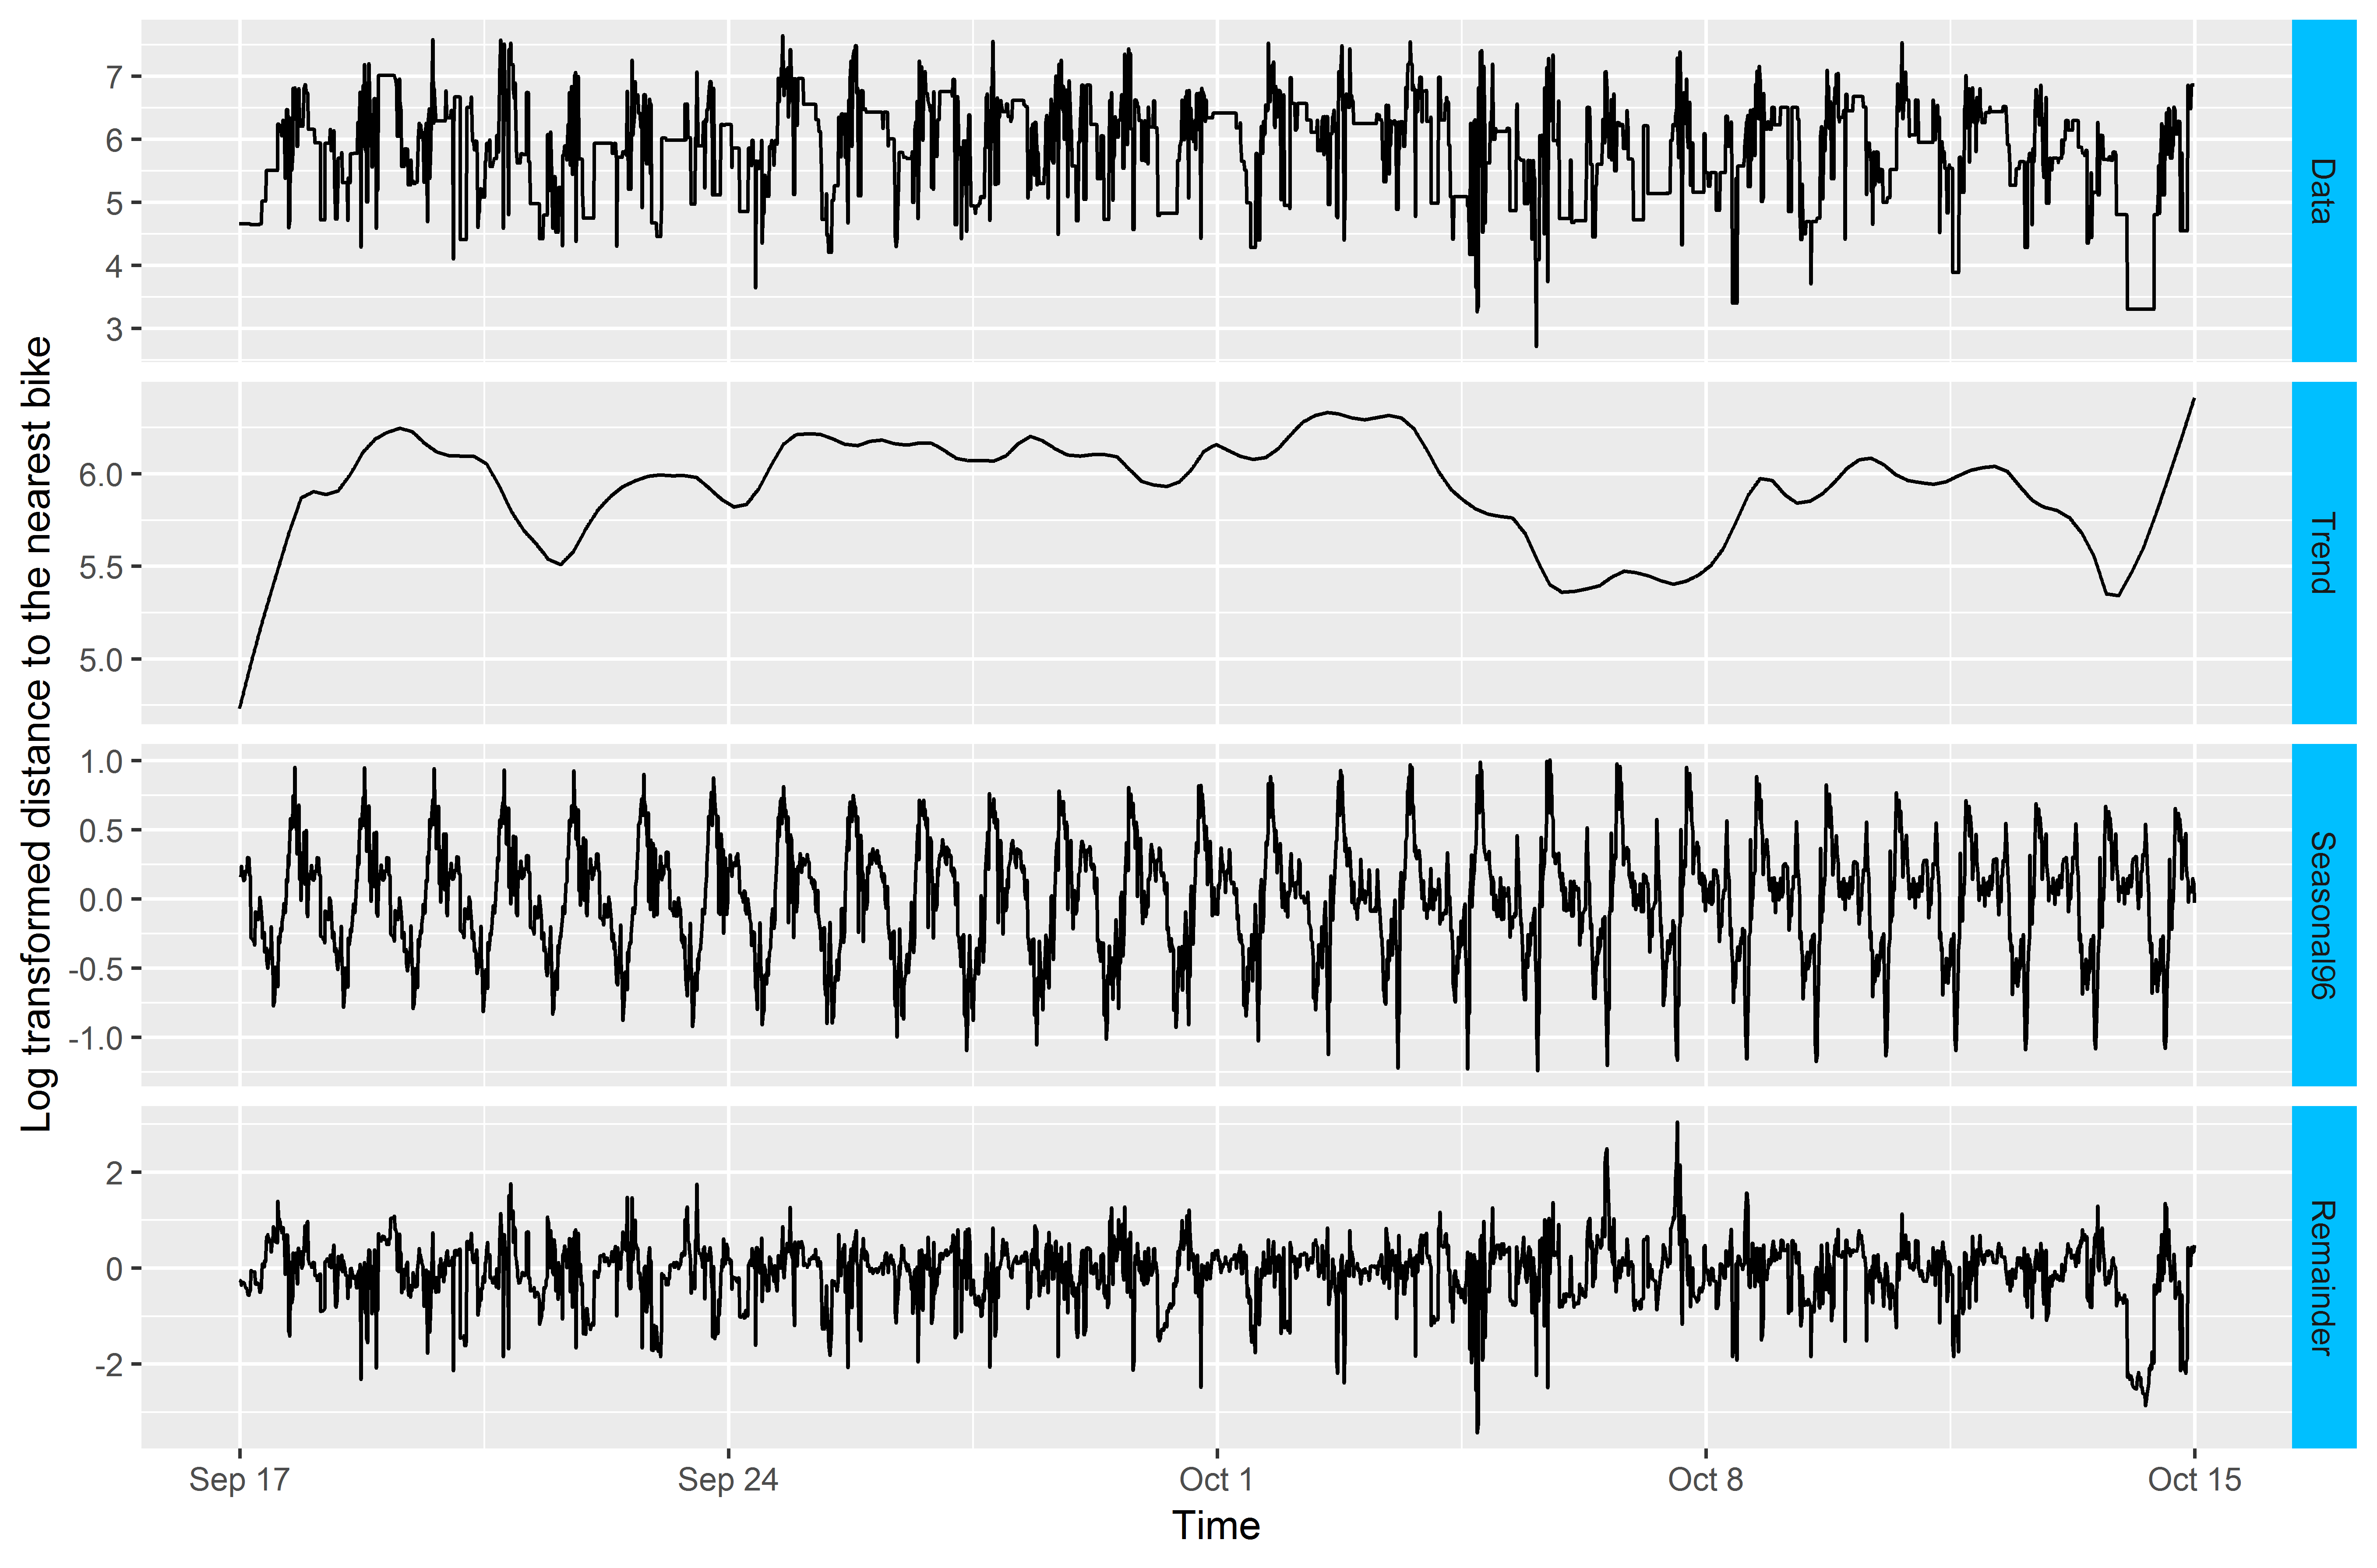
\includegraphics[width=\textwidth]{Figures/stlplot_model2}

\textbf{Model}
\begin{verbatim}
Series: x 
ARIMA(3,1,2) 

Coefficients:
          ar1     ar2     ar3      ma1     ma2
      -0.1423  0.5707  0.1873  -0.2605  -0.719
s.e.   0.3526  0.2258  0.0351   0.3600   0.352

sigma^2 estimated as 0.2219:  log likelihood=-1788.92
AIC=3589.84   AICc=3589.87   BIC=3625.22
\end{verbatim}
\newpage

\section{Residential model point}\label{residential-model-point}

\textbf{Decomposition plot}

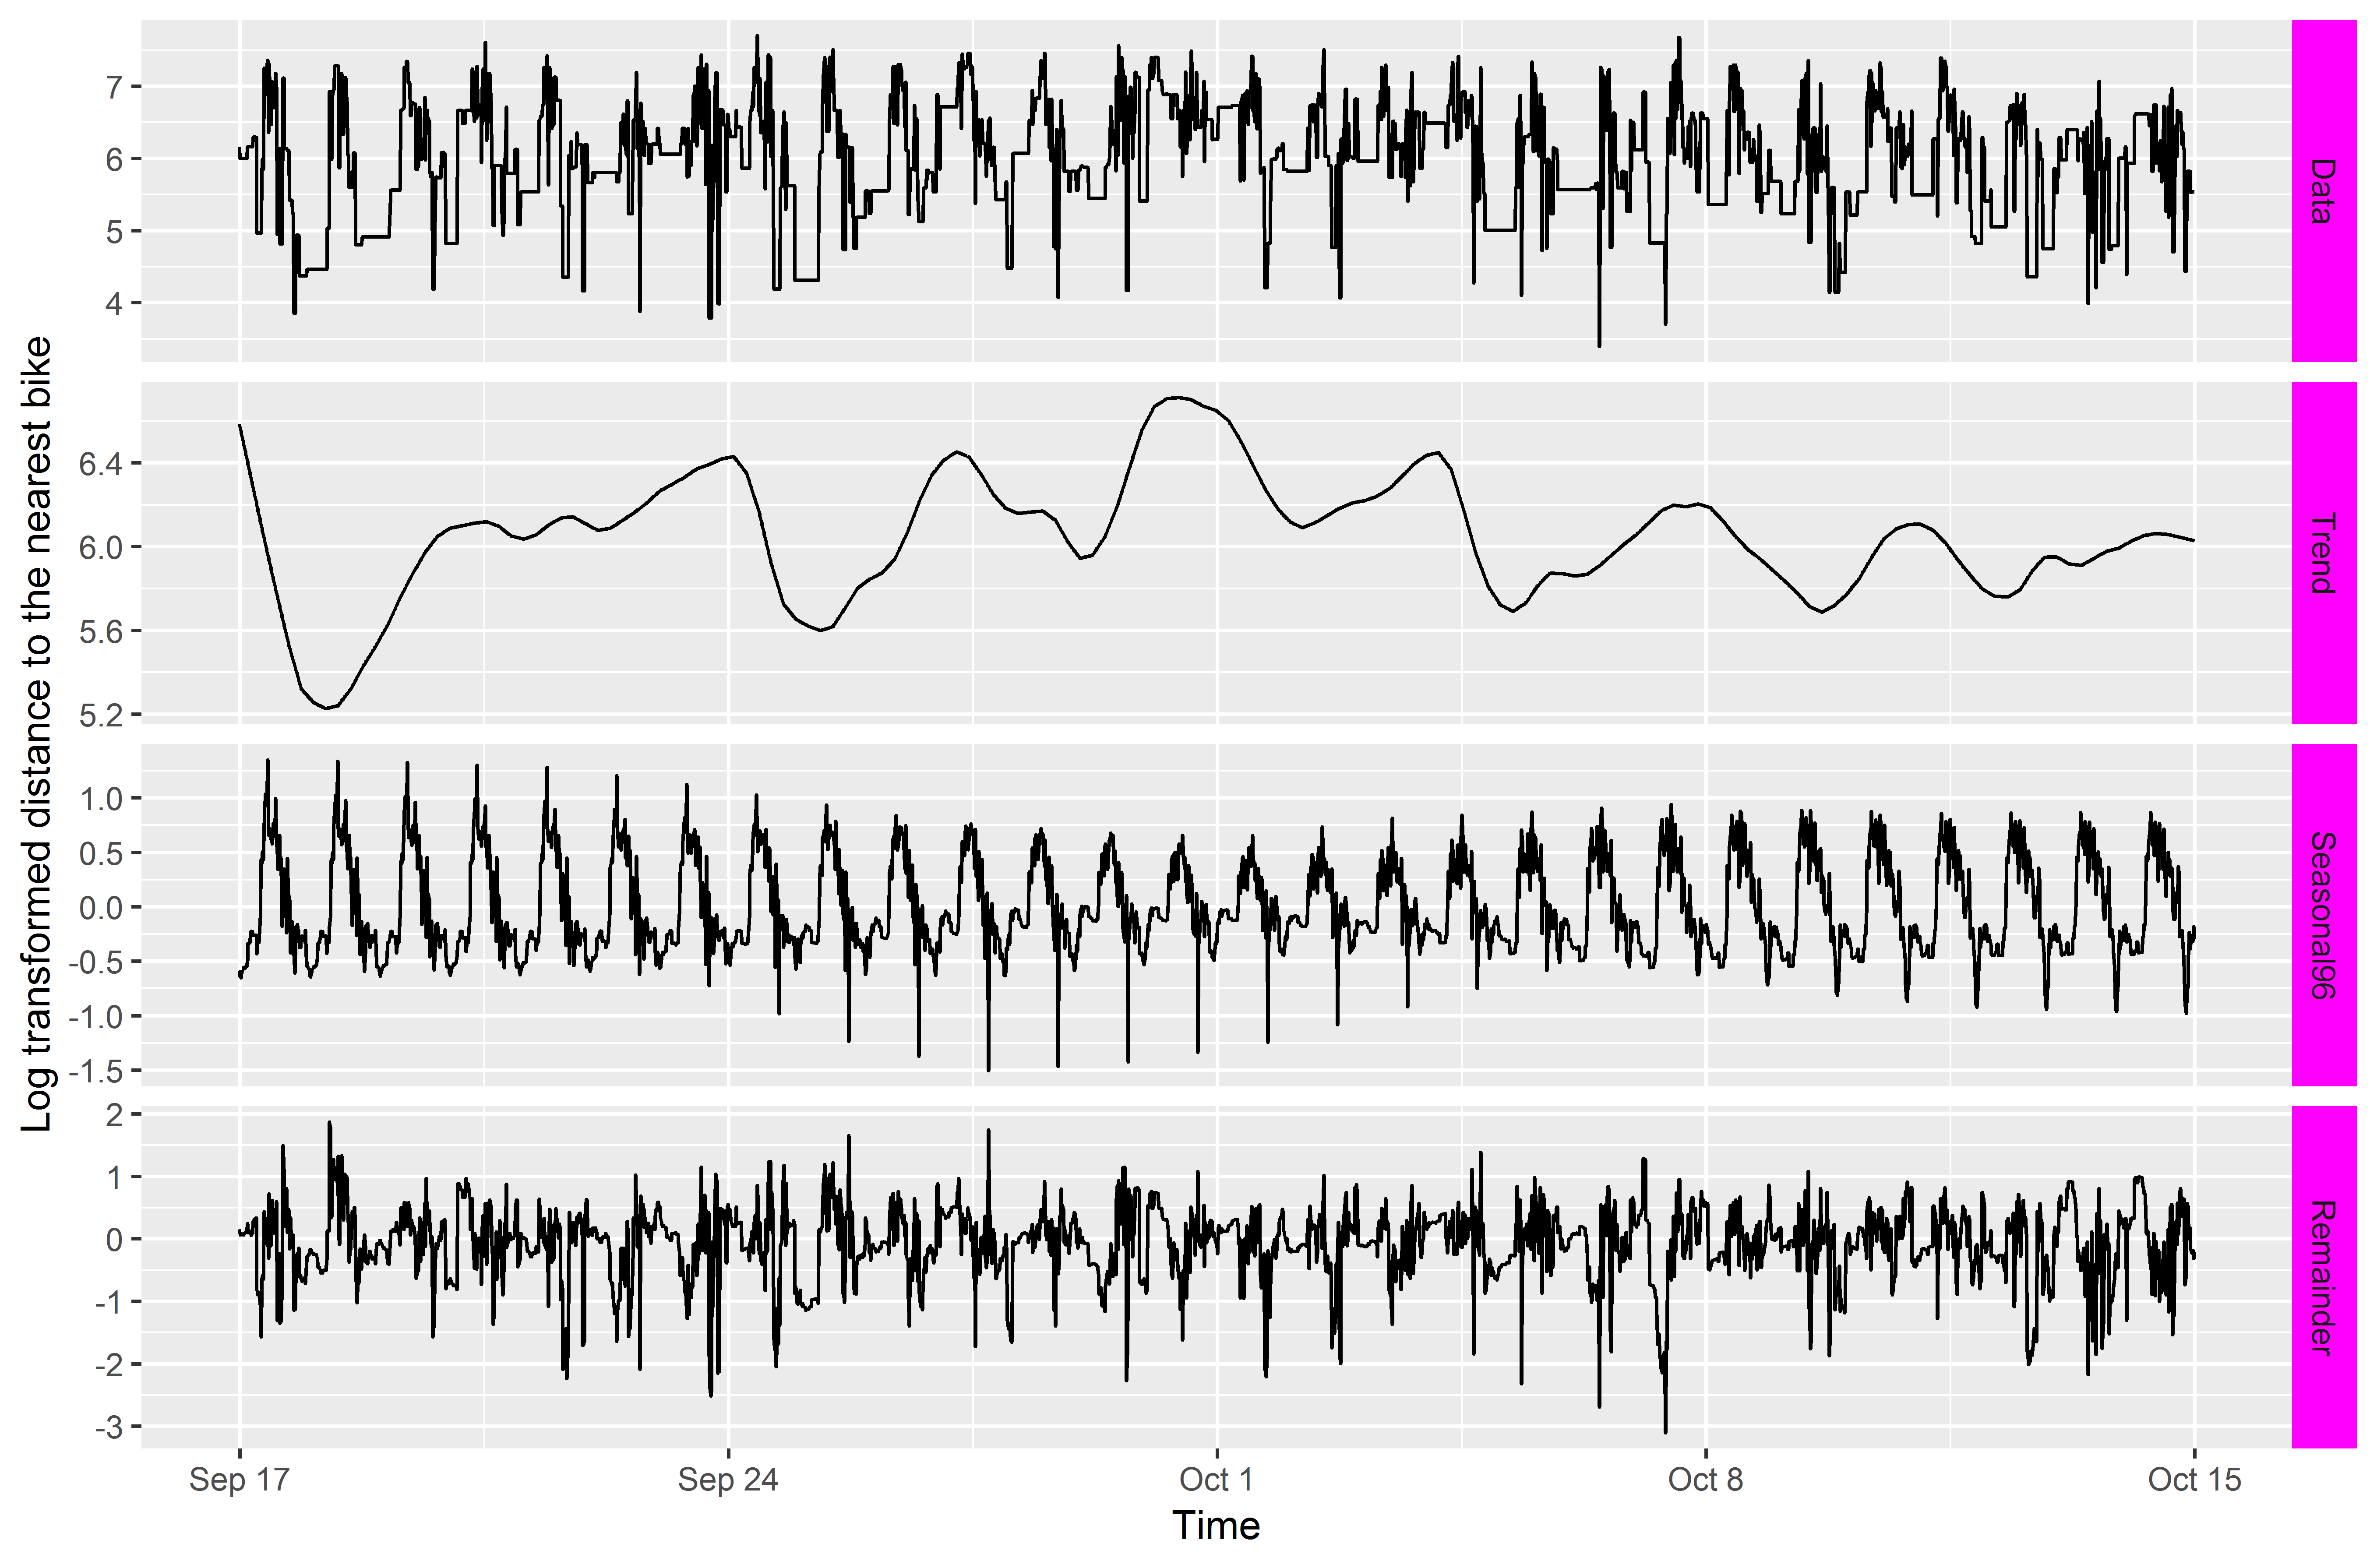
\includegraphics[width=\textwidth]{Figures/stlplot_model3}

\textbf{Model}
\begin{verbatim}
Series: x 
ARIMA(1,1,1) 

Coefficients:
         ar1      ma1
      0.6263  -0.9128
s.e.  0.0394   0.0257

sigma^2 estimated as 0.1714:  log likelihood=-1442.62
AIC=2891.25   AICc=2891.26   BIC=2908.94
\end{verbatim}
\newpage

\section{Presidio model point}\label{presidio-model-point}

\textbf{Decomposition plot}

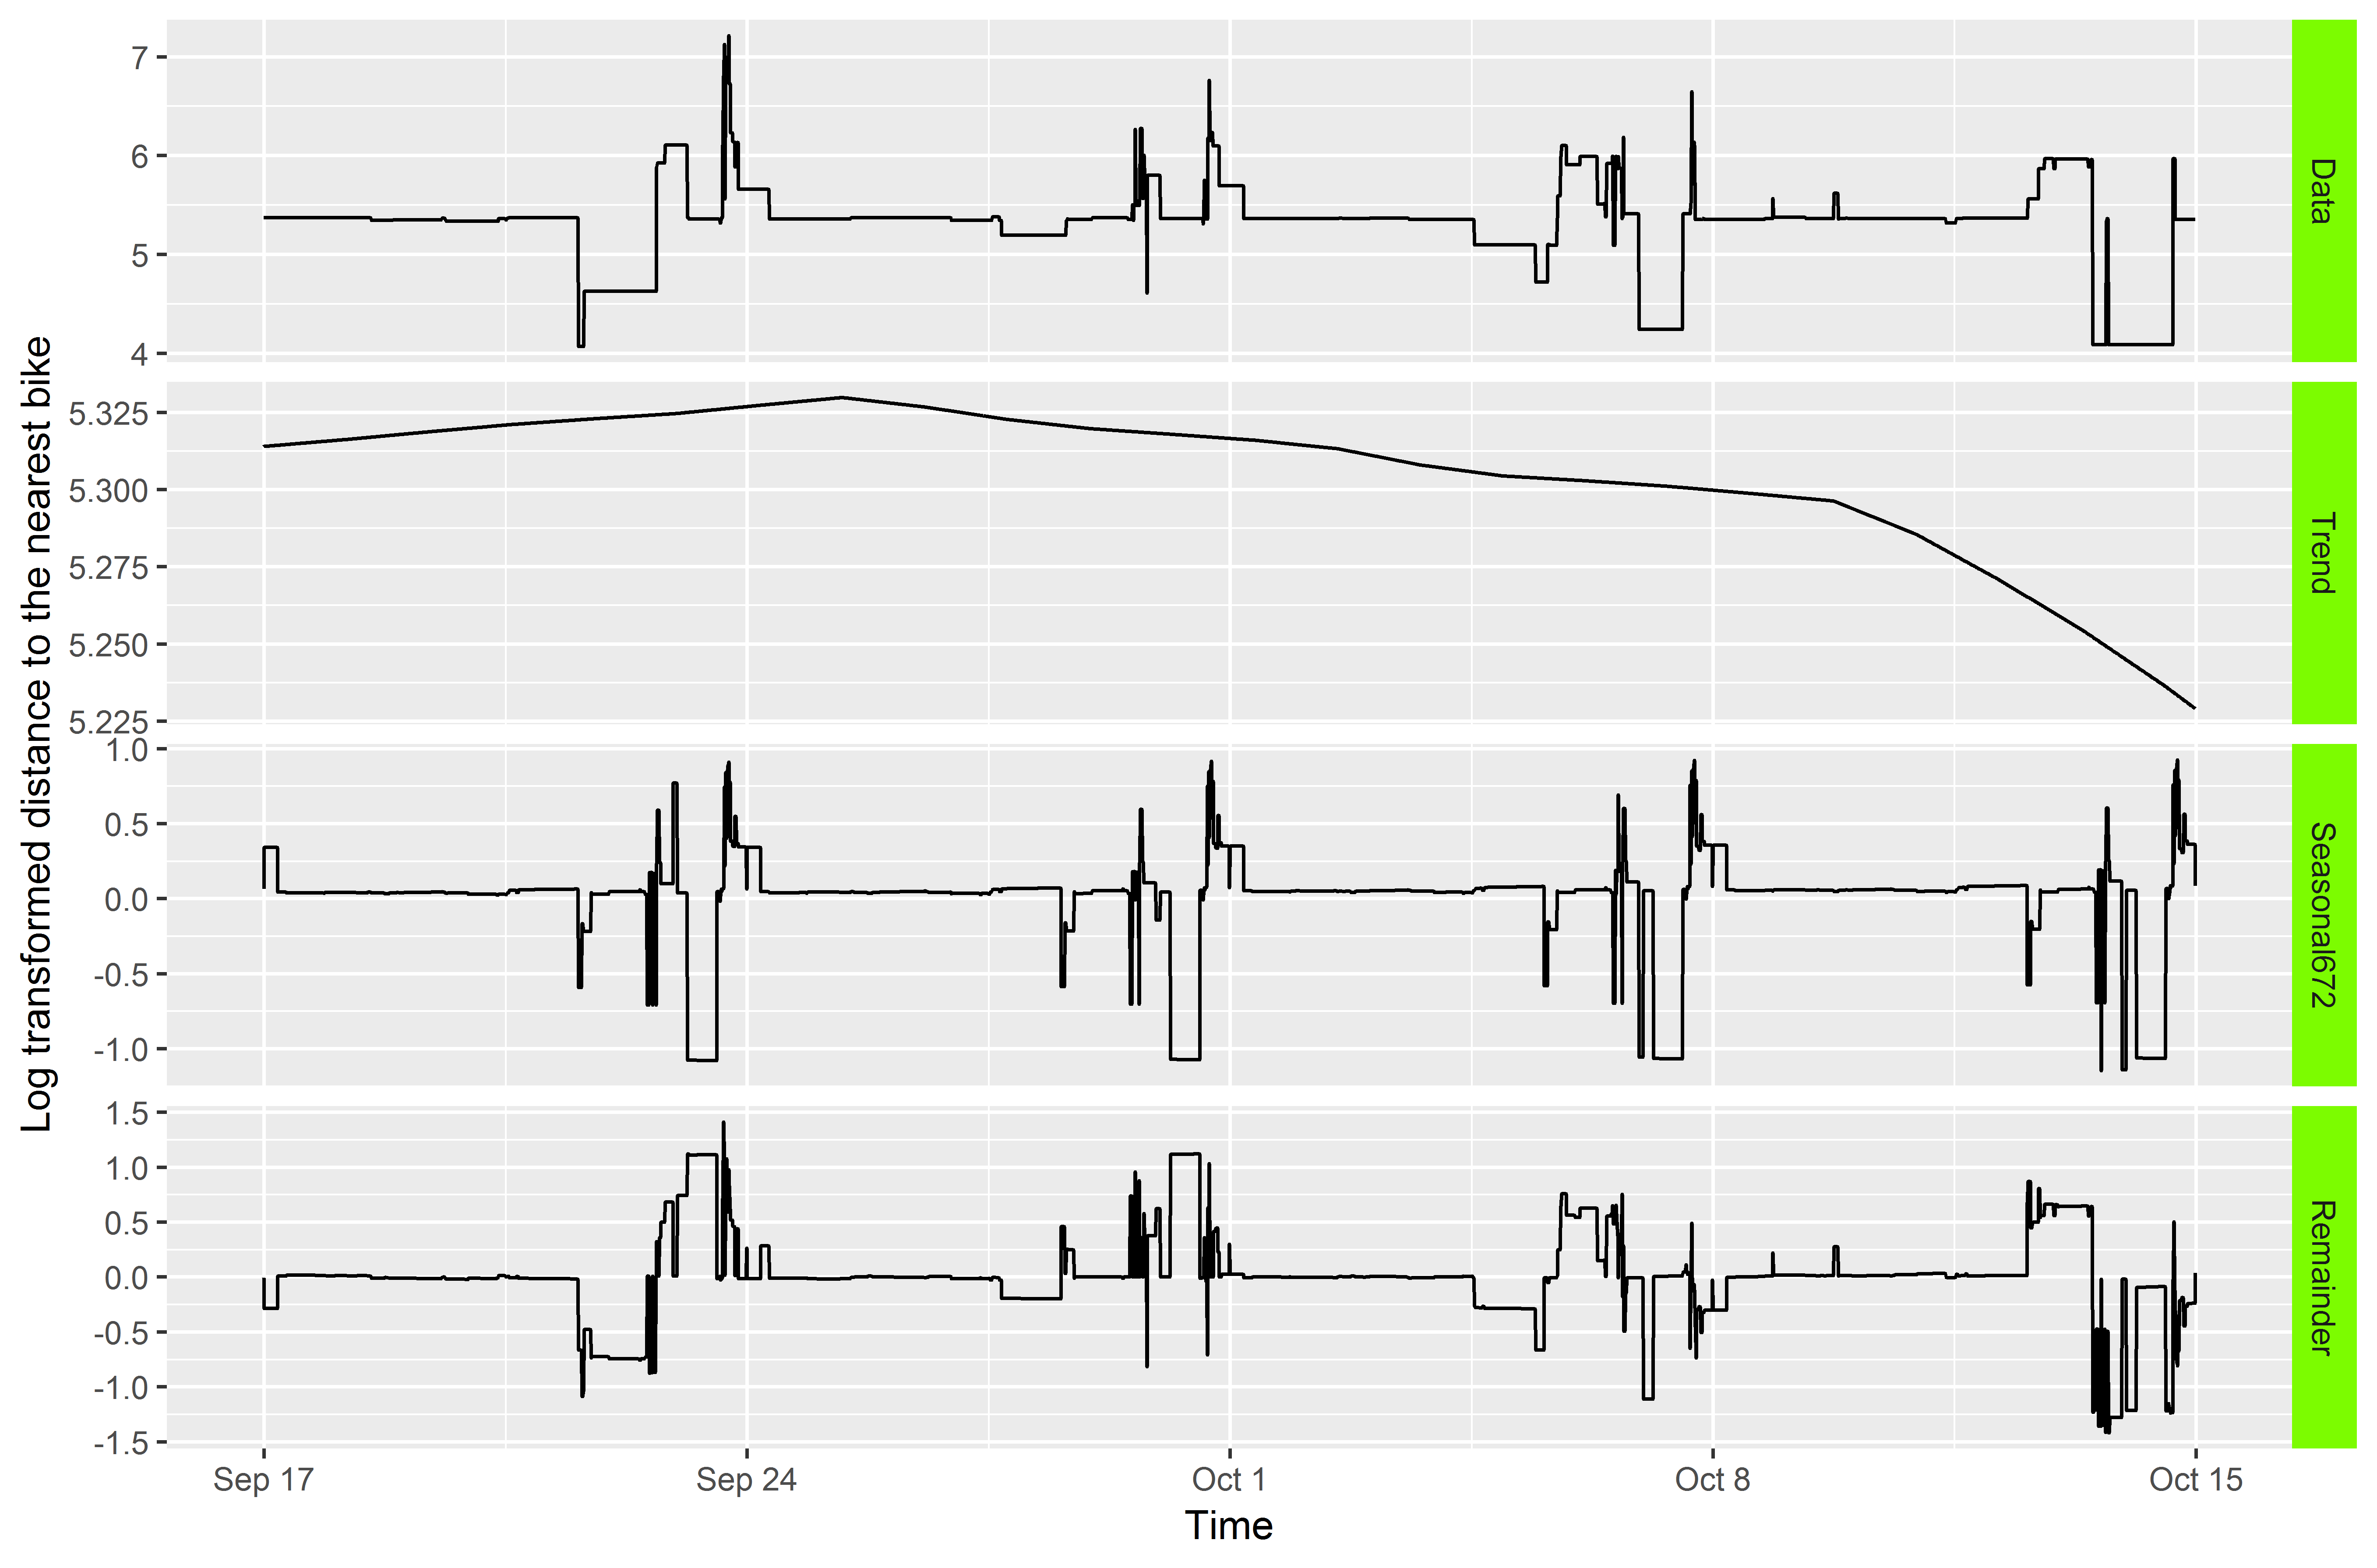
\includegraphics[width=\textwidth]{Figures/stlplot_model4}

\textbf{Model}
\begin{verbatim}
Series: x 
ARIMA(1,1,4) 

Coefficients:
          ar1     ma1      ma2      ma3      ma4
      -0.6904  0.4389  -0.2201  -0.1439  -0.1430
s.e.   0.0781  0.0790   0.0275   0.0232   0.0192

sigma^2 estimated as 0.02021:  log likelihood=1431.7
AIC=-2851.41   AICc=-2851.37   BIC=-2816.03
\end{verbatim}
\backmatter

\chapter*{References}\label{references}
\addcontentsline{toc}{chapter}{References}

\markboth{References}{References}

\noindent

\setlength{\parindent}{-0.20in} \setlength{\leftskip}{0.20in}
\setlength{\parskip}{8pt}

\hypertarget{refs}{}
\hypertarget{ref-anselin2010}{}
Anselin, L. (2010). Thirty years of spatial econometrics. \emph{Papers
in Regional Science}, \emph{89}(1), 3--25.
\url{http://doi.org/10.1111/j.1435-5957.2010.00279.x}

\hypertarget{ref-bbc}{}
Belton, P. (2018, May). How cheap dockless hire bikes are flooding the
world. Retrieved from \url{https://www.bbc.com/news/business-44066083}

\hypertarget{ref-borgnat2011}{}
Borgnat, P., Robardet, C., Rouquier, J.-B., Abry, P., Flandrin, P., \&
Fleury, E. (2011). Shared Bicycles in a City: A Signal Processing and
Data Analysis Perspective. \emph{Advances in Complex Systems},
\emph{14}. \url{http://doi.org/10.1142/S0219525911002950}

\hypertarget{ref-box1970}{}
Box, G. E. P., \& Jenkins, G. M. (1970). \emph{Time Series Analysis:
Forecasting and Control}. Book, Holden-Day San Francisco.

\hypertarget{ref-clValid}{}
Brock, G., Pihur, V., Datta, S., \& Datta, S. (2008). clValid: An R
Package for Cluster Validation. \emph{Journal of Statistical Software},
\emph{25}(4), 1--22. Retrieved from
\url{http://www.jstatsoft.org/v25/i04/}

\hypertarget{ref-brockwell2002}{}
Brockwell, P. J., \& Davis, R. A. (2002). \emph{An Introduction to Time
Series and Forecasting} (Vol. 39).
\url{http://doi.org/10.1007/978-1-4757-2526-1}

\hypertarget{ref-caggiani2017}{}
Caggiani, L., Ottomanelli, M., Camporeale, R., \& Binetti, M. (2017).
Spatio-temporal clustering and forecasting method for free-floating bike
sharing systems. In \emph{Advances in intelligent systems and computing}
(Vol. 539, pp. 244--254). Springer Verlag. Retrieved from
\href{http://dx.doi.org/10.1007/978-3-319-48944-5\%7B/_\%7D23}{http://dx.doi.org/10.1007/978-3-319-48944-5\{\textbackslash{}\_\}23}

\hypertarget{ref-campbell2016}{}
Campbell, A. A., Cherry, C. R., Ryerson, M. S., \& Yang, X. (2016).
Factors influencing the choice of shared bicycles and shared electric
bikes in Beijing. \emph{Transportation Research Part C: Emerging
Technologies}, \emph{67}, 399--414.
\url{http://doi.org/https://doi.org/10.1016/j.trc.2016.03.004}

\hypertarget{ref-carto}{}
CARTO. (2018). Attribution: Powered by CARTO. Retrieved from
\url{https://carto.com/attribution/}

\hypertarget{ref-cassisi2012}{}
Cassisi, C., Montalto, P., Aliotta, M., Cannata, A., \& Pulvirenti, A.
(2012). Similarity Measures and Dimensionality Reduction Techniques for
Time Series Data Mining. In. \url{http://doi.org/10.5772/49941}

\hypertarget{ref-chai2014}{}
Chai, T., \& Draxler, R. R. (2014). Root mean square error (RMSE) or
mean absolute error (MAE)? Arguments against avoiding RMSE in the
literature. \emph{Geoscientific Model Development}, \emph{7}(3),
1247--1250. \url{http://doi.org/10.5194/gmd-7-1247-2014}

\hypertarget{ref-clustgeo}{}
Chavent, M., Kuentz-Simonet, V., Labenne, A., \& Saracco, J. (2018).
ClustGeo: an R package for hierarchical clustering with spatial
constraints. \emph{Computational Statistics}, \emph{33}(4), 1799--1822.
\url{http://doi.org/10.1007/s00180-018-0791-1}

\hypertarget{ref-cleveland1990}{}
Cleveland, R. B., Cleveland, W. S., McRae, J. E., \& Terpenning, I.
(1990). STL: A Seasonal-Trend Decomposition Procedure Based On Loess.
\emph{Journal of Official Statistics}, \emph{6}(1), 3--73.

\hypertarget{ref-cleveland1988}{}
Cleveland, W. S., \& Devlin, S. J. (1988). Locally Weighted Regression:
An Approach to Regression Analysis by Local Fitting. \emph{Journal of
the American Statistical Association}, \emph{83}(403), 596--610.
\url{http://doi.org/10.1080/01621459.1988.10478639}

\hypertarget{ref-guardian2}{}
Collinson, P. (2018, March). Bike wars: Chinese bike-share giants wheel
out UK expansion plans. Retrieved from
\url{https://www.theguardian.com/uk-news/2018/mar/12/bike-wars-chinese-bike-share-giants-wheel-out-expansion-plans-in-uk}

\hypertarget{ref-RPostgreSQL}{}
Conway, J., Eddelbuettel, D., Nishiyama, T., Prayaga, S. K., \& Tiffin,
N. (2017). \emph{RPostgreSQL: R Interface to the 'PostgreSQL' Database
System}. Retrieved from
\url{https://cran.r-project.org/package=RPostgreSQL}

\hypertarget{ref-corcoran2014}{}
Corcoran, J., Li, T., Rohde, D., Charles-Edwards, E., \& Mateo-Babiano,
D. (2014). Spatio-temporal patterns of a Public Bicycle Sharing Program:
the effect of weather and calendar events. \emph{Journal of Transport
Geography}, \emph{41}, 292--305.
\url{http://doi.org/https://doi.org/10.1016/j.jtrangeo.2014.09.003}

\hypertarget{ref-dambolena2009}{}
Dambolena, I. G., Eriksen, S. E., \& Kopcso, D. P. (2009). Logarithmic
Transformations in Regression: Do You Transform Back Correctly?
\emph{PRIMUS}, \emph{19}(3), 280--295.
\url{http://doi.org/10.1080/10511970802234976}

\hypertarget{ref-itf2018}{}
Deighton-Smith, R. (2018). \emph{The Economics of Regulating
Ride-Hailing and Dockless Bike Share}. International Transport Forum.
Retrieved from
\url{https://www.itf-oecd.org/economics-regulating-ride-hailing-and-dockless-bike-share}

\hypertarget{ref-demaio2009}{}
DeMaio, P. (2009). Bike-sharing: History, Impacts, Models of Provision,
and Future. \emph{Journal of Public Transportation}, \emph{12}(4).
\url{http://doi.org/10.5038/2375-0901.12.4.3}

\hypertarget{ref-dias2015}{}
Dias, G. M., Bellalta, B., \& Oechsner, S. (2015). Predicting occupancy
trends in Barcelona's bicycle service stations using open data. In
\emph{2015 sai intelligent systems conference (intellisys)} (pp.
439--445). \url{http://doi.org/10.1109/IntelliSys.2015.7361177}

\hypertarget{ref-dunn1974}{}
Dunn, J. C. (1974). Well-Separated Clusters and Optimal Fuzzy
Partitions. \emph{Journal of Cybernetics}, \emph{4}(1), 95--104.
\url{http://doi.org/10.1080/01969727408546059}

\hypertarget{ref-rosm}{}
Dunnington, D. (2017). \emph{rosm: Plot Raster Map Tiles from Open
Street Map and Other Sources}. Retrieved from
\url{https://cran.r-project.org/package=rosm}

\hypertarget{ref-ggspatial}{}
Dunnington, D. (2018). \emph{ggspatial: Spatial Data Framework for
ggplot2}. Retrieved from
\url{https://cran.r-project.org/package=ggspatial}

\hypertarget{ref-tz}{}
Eggert, P., \& Olson, A. D. (2018). Sources for Time Zone and Daylight
Saving Time Data. Retrieved from
\url{https://data.iana.org/time-zones/tz-link.html}

\hypertarget{ref-ermagun2018}{}
Ermagun, A., \& Levinson, D. (2018). Spatiotemporal traffic forecasting:
review and proposed directions. \emph{Transport Reviews}, \emph{38}(6),
786--814. \url{http://doi.org/10.1080/01441647.2018.1442887}

\hypertarget{ref-faghih2014}{}
Faghih-Imani, A., Eluru, N., El-Geneidy, A. M., Rabbat, M., \& Haq, U.
(2014). How land-use and urban form impact bicycle flows: evidence from
the bicycle-sharing system (BIXI) in Montreal. \emph{Journal of
Transport Geography}, \emph{41}, 306--314.
\url{http://doi.org/https://doi.org/10.1016/j.jtrangeo.2014.01.013}

\hypertarget{ref-fishman2016}{}
Fishman, E. (2016). Cycling as transport. \emph{Transport Reviews},
\emph{36}(1), 1--8. \url{http://doi.org/10.1080/01441647.2015.1114271}

\hypertarget{ref-fishman2014}{}
Fishman, E., Washington, S., Haworth, N., \& Mazzei, A. (2014). Barriers
to bikesharing: an analysis from Melbourne and Brisbane. \emph{Journal
of Transport Geography}, \emph{41}, 325--337.
\url{http://doi.org/https://doi.org/10.1016/j.jtrangeo.2014.08.005}

\hypertarget{ref-foley2018}{}
Foley, N. (2018, December). Getting more people on JUMP bikes with our
new design. Retrieved from \url{https://www.uber.com/newsroom/newbike/}

\hypertarget{ref-formentin2015}{}
Formentin, S., Bianchessi, A. G., \& Savaresi, S. M. (2015). On the
prediction of future vehicle locations in free-floating car sharing
systems. In \emph{2015 ieee intelligent vehicles symposium (iv)} (pp.
1006--1011). \url{http://doi.org/10.1109/IVS.2015.7225816}

\hypertarget{ref-froehlich2009}{}
Froehlich, J., Neumann, J., \& Oliver, N. (2009). Sensing and predicting
the pulse of the city through shared bicycling. \emph{IJCAI
International Joint Conference on Artificial Intelligence}, (3),
1420--1426. \url{http://doi.org/10.1.1.150.4370}

\hypertarget{ref-gan2007}{}
Gan, G., Ma, C., \& Wu, J. (2007). \emph{Data Clustering: Theory,
Algorithms, and Applications}. Society for Industrial; Applied
Mathematics.

\hypertarget{ref-giot2014}{}
Giot, R., \& Cherrier, R. (2014). Predicting bikeshare system usage up
to one day ahead. In \emph{2014 ieee symposium on computational
intelligence in vehicles and transportation systems (civts)} (pp.
22--29). \url{http://doi.org/10.1109/CIVTS.2014.7009473}

\hypertarget{ref-goerg2013}{}
Goerg, G. M. (2013). Forecastable Component Analysis. \emph{Proceedings
of the 30th International Conference on Machine Learning, ICML 2013},
64--72. Retrieved from \url{arxiv:1205.4591}

\hypertarget{ref-goodman2014}{}
Goodman, A., Green, J., \& Woodcock, J. (2014). The role of bicycle
sharing systems in normalising the image of cycling: An observational
study of London cyclists. \emph{Journal of Transport \& Health},
\emph{1}(1), 5--8.
\url{http://doi.org/https://doi.org/10.1016/j.jth.2013.07.001}

\hypertarget{ref-lubridate}{}
Grolemund, G., \& Wickham, H. (2011). Dates and Times Made Easy with
lubridate. \emph{Journal of Statistical Software}, \emph{40}(3), 1--25.
Retrieved from \url{http://www.jstatsoft.org/v40/i03/}

\hypertarget{ref-harris2018}{}
Harris, D. (2018, June). The Complete San Francisco Bikeshare Review
Guide. Retrieved from
\url{https://biketoeverything.com/2018/06/12/complete-san-francisco-bikeshare-review/}

\hypertarget{ref-hickman2014}{}
Hickman, R., \& Banister, D. (2014). \emph{Transport, Climate Change and
the City}. Taylor \& Francis.

\hypertarget{ref-huang2000}{}
Huang, J., \& Pawitan, Y. (2000). Quasi-Likelihood Estimation of
Non-Invertible Moving Average Processes. \emph{Scandinavian Journal of
Statistics}, \emph{27}(4), 689--702. Retrieved from
\url{http://www.jstor.org/stable/4616635}

\hypertarget{ref-hyndmanblog}{}
Hyndman, R. J. (2010). Forecasting with long seasonal periods. Retrieved
from \url{https://robjhyndman.com/hyndsight/longseasonality/}

\hypertarget{ref-hyndman2018fpp}{}
Hyndman, R. J., \& Athanasopoulos, G. (2018). \emph{Forecasting:
principles and practice}. OTexts. Retrieved from
\url{https://otexts.org/fpp2/}

\hypertarget{ref-forecast}{}
Hyndman, R. J., \& Khandakar, Y. (2008). Automatic time series
forecasting: the forecast package for R. \emph{Journal of Statistical
Software}, \emph{26}(3), 1--22. Retrieved from
\url{http://www.jstatsoft.org/article/view/v027i03}

\hypertarget{ref-tsfeatures}{}
Hyndman, R. J., Kang, Y., Talagala, T., Wang, E., \& Yang, Y. (2019).
\emph{tsfeatures: Time Series Feature Extraction}. Retrieved from
\url{https://pkg.robjhyndman.com/tsfeatures/}

\hypertarget{ref-tsibblestats}{}
Hyndman, R. J., O'Hara-Wild, M., \& Wang, E. (2018). \emph{tsibblestats:
Analysis of tidy time series}. Retrieved from
\url{https://github.com/tidyverts/tsibblestats}

\hypertarget{ref-iliffe2008}{}
Iliffe, J., \& Lott, R. (2008). \emph{Datums and Map Projections: For
Remote Sensing, GIS and Surveying}. Whittles Pub.

\hypertarget{ref-sfmta2018one}{}
Jose, B. (2018a, January). SFMTA Creates Pilot to Study Electric,
Stationless Bike Sharing. Retrieved from
\url{https://www.sfmta.com/blog/sfmta-creates-pilot-study-electric-stationless-bike-sharing}

\hypertarget{ref-sfmta2018two}{}
Jose, B. (2018b, September). San Francisco's Stationless Bikeshare Pilot
Reaches Mid-Point Milestone. Retrieved from
\url{https://www.sfmta.com/blog/san-franciscos-stationless-bikeshare-pilot-reaches-mid-point-milestone}

\hypertarget{ref-kaggle}{}
Kaggle. (2014). Bike Sharing Demand: Forecast use of a city bikeshare
system. Retrieved from
\url{https://www.kaggle.com/c/bike-sharing-demand}

\hypertarget{ref-kaltenbrunner2010}{}
Kaltenbrunner, A., Meza, R., Grivolla, J., Codina, J., \& Banchs, R.
(2010). Urban cycles and mobility patterns: Exploring and predicting
trends in a bicycle-based public transport system. \emph{Pervasive and
Mobile Computing}, \emph{6}(4), 455--466.
\url{http://doi.org/10.1016/j.pmcj.2010.07.002}

\hypertarget{ref-kamarianakis2005}{}
Kamarianakis, Y., \& Prastacos, P. (2005). Spatial time-series modeling:
A review of the proposed methodologies. In \emph{Proceedings 2005 - the
8th agile international conference on geographic information science,
agile 2005}.

\hypertarget{ref-keogh2005}{}
Keogh, E., \& Lin, J. (2005). Clustering of time-series subsequences is
meaningless: Implications for previous and future research.
\emph{Knowledge and Information Systems}, \emph{8}, 154--177.
\url{http://doi.org/10.1007/s10115-004-0172-7}

\hypertarget{ref-uber2018}{}
Khosrowshahi, D. (2018, April). Welcome, JUMP! Retrieved from
\url{https://www.uber.com/newsroom/welcomejump/}

\hypertarget{ref-kwiat1992}{}
Kwiatkowski, D., Phillips, P. C. B., Schmidt, P., \& Shin, Y. (1992).
Testing the null hypothesis of stationarity against the alternative of a
unit root: How sure are we that economic time series have a unit root?
\emph{Journal of Econometrics}, \emph{54}(1), 159--178.
\url{http://doi.org/https://doi.org/10.1016/0304-4076(92)90104-Y}

\hypertarget{ref-nytimes}{}
Larmer, B. (2017, November). China's Revealing Spin on the `Sharing
Economy'. Retrieved from
\url{https://www.nytimes.com/2017/11/20/magazine/chinas-revealing-spin-on-the-sharing-economy.html}

\hypertarget{ref-lehr1998}{}
Lehr, M. E., \& Lii, K.-S. (1998). Maximum Likelihood Estimates of
Non-Gaussian ARMA Models. \emph{1998 Symposium on Nonlinear Time Series
Models}. Retrieved from
\href{https://eml.berkeley.edu/symposia/nsf98/lii\%7B/_\%7Dlehr.pdf}{https://eml.berkeley.edu/symposia/nsf98/lii\{\textbackslash{}\_\}lehr.pdf}

\hypertarget{ref-li1988}{}
Li, W. K., \& McLeod, A. I. (1988). ARMA modelling with non-gaussian
innovations. \emph{Journal of Time Series Analysis}, \emph{9}(2),
155--168. \url{http://doi.org/10.1111/j.1467-9892.1988.tb00461.x}

\hypertarget{ref-li2015}{}
Li, Y., Zheng, Y., Zhang, H., \& Chen, L. (2015). Traffic prediction in
a bike-sharing system. In \emph{23rd sigspatial international
conference} (pp. 1--10). \url{http://doi.org/10.1145/2820783.2820837}

\hypertarget{ref-lin2018}{}
Lin, L., He, Z., \& Peeta, S. (2018). Predicting station-level hourly
demand in a large-scale bike-sharing network: A graph convolutional
neural network approach. \emph{Transportation Research Part C: Emerging
Technologies}, \emph{97}, 258--276.
\url{http://doi.org/https://doi.org/10.1016/j.trc.2018.10.011}

\hypertarget{ref-lozano2018}{}
Lozano, Á., Paz, J. F. D., Villarrubia, G., De La Iglesia, D. H., \&
Bajo, J. (2018). Multi-Agent System for Demand Prediction and Trip
Visualization in Bike Sharing Systems. \emph{Applied Sciences},
\emph{8}(1), 67. \url{http://doi.org/10.3390/app8010067}

\hypertarget{ref-mccullough1994}{}
McCullough, B. D. (1994). Bootstrapping forecast intervals: An
application to AR(p) models. \emph{Journal of Forecasting},
\emph{13}(1), 51--66. \url{http://doi.org/10.1002/for.3980130107}

\hypertarget{ref-mckenzie2018}{}
Mckenzie, G. (2018). Docked vs. Dockless Bike-sharing : Contrasting
Spatiotemporal Patterns. In \emph{10th international conference on
geographic information science (giscience 2018)} (pp. 46:1-----46:7).
\url{http://doi.org/10.4230/LIPIcs.GISCIENCE.2018.46}

\hypertarget{ref-muller2015}{}
Müller, J., \& Bogenberger, K. (2015). Time Series Analysis of Booking
Data of a Free-Floating Carsharing System in Berlin.
\emph{Transportation Research Procedia}, \emph{10}, 345--354.
\url{http://doi.org/https://doi.org/10.1016/j.trpro.2015.09.084}

\hypertarget{ref-tibble}{}
Müller, K., \& Wickham, H. (2019). \emph{tibble: Simple Data Frames}.
Retrieved from \url{https://cran.r-project.org/package=tibble}

\hypertarget{ref-nacto2018}{}
NACTO. (2018). \emph{Bike Share in the U.S.: 2017}. National Association
of City Transportation Officials. Retrieved from
\url{https://nacto.org/wp-content/uploads/2018/05/NACTO-Bike-Share-2017.pdf}

\hypertarget{ref-nau2018}{}
Nau, R. (2018). Stationarity and differencing of time series data.
Retrieved from
\href{https://people.duke.edu/\%7B~\%7Drnau/411diff.htm}{https://people.duke.edu/\{\textasciitilde{}\}rnau/411diff.htm}

\hypertarget{ref-fasster}{}
O'Hara-Wild, M. (2018). \emph{fasster: Fast Additive Switching of
Seasonality, Trend and Exogenous Regressors}. Retrieved from
\url{https://github.com/mitchelloharawild/fasster}

\hypertarget{ref-pal2018}{}
Pal, A., Zhang, Y., \& Kwon, C. (2018). \emph{Analysis of Free-floating
Bike Sharing and Insights on System Operations}. Civil; Environmental
Engineering University of South Florida. Retrieved from
\url{https://hdl.handle.net/1813/56569}

\hypertarget{ref-sf}{}
Pebesma, E. (2018). Simple Features for R: Standardized Support for
Spatial Vector Data. \emph{The R Journal}. Retrieved from
\url{https://journal.r-project.org/archive/2018/RJ-2018-009/index.html}

\hypertarget{ref-postgres}{}
PostgreSQL. (2014). PostgreSQL: The world's most advanced open source
database. Retrieved from \url{http://www.postgresql.org/}

\hypertarget{ref-proj}{}
PROJ-contributors. (2018). \emph{PROJ coordinate transformation software
library}. Open Source Geospatial Foundation. Retrieved from
\url{https://proj4.org/}

\hypertarget{ref-pucher2017}{}
Pucher, J., \& Buehler, R. (2017). Cycling towards a more sustainable
transport future. \emph{Transport Reviews}, \emph{37}(6), 689--694.
\url{http://doi.org/10.1080/01441647.2017.1340234}

\hypertarget{ref-rlanguage}{}
R Core Team. (2013). \emph{R: A Language and Environment for Statistical
Computing}. Vienna, Austria: R Foundation for Statistical Computing.
Retrieved from \url{http://www.r-project.org/}

\hypertarget{ref-rixley2013}{}
Rixey, A. R. (2013). Station-Level Forecasting of Bikesharing Ridership.
\emph{Transportation Research Record: Journal of the Transportation
Research Board}, \emph{2387}, 46--55.
\url{http://doi.org/10.3141/2387-06}

\hypertarget{ref-ruffieux2017}{}
Ruffieux, S., Spycher, N., Mugellini, E., \& Khaled, O. A. (2017).
Real-time usage forecasting for bike-sharing systems: A study on random
forest and convolutional neural network applicability. In \emph{2017
intelligent systems conference (intellisys)} (pp. 622--631).
\url{http://doi.org/10.1109/IntelliSys.2017.8324359}

\hypertarget{ref-jump2019}{}
Rzepecki, R. (2019, February). Celebrating One Year in San Francisco.
Retrieved from
\url{https://medium.com/@jumpbikes/celebrating-one-year-in-san-francisco-28469d5dccaa}

\hypertarget{ref-sfindicator}{}
San Francisco Department of Public Health. (2014). The San Francisco
Indicator Project. Retrieved from
\url{https://www.sfindicatorproject.org/}

\hypertarget{ref-schmidt2018}{}
Schmidt, C. (2018). Active Travel for All? The Surge in Public
Bike-Sharing Programs. \emph{Environmental Health Perspectives},
\emph{126}, 82001. \url{http://doi.org/10.1289/EHP3754}

\hypertarget{ref-sfmta2018three}{}
SFMTA Board of Directors. (2018). \emph{Stationless Bikeshare Pilot
Midpoint Evaluation}. San Francisco Municipal Transportation Agency.
Retrieved from
\url{https://techcrunch.com/2018/10/01/ubers-jump-bike-fleet-may-soon-double-in-size-in-sf/}

\hypertarget{ref-shaheen2010}{}
Shaheen, S., Guzman, S., \& Zhang, H. (2010). Bikesharing in Europe, the
Americas, and Asia: Past, Present, and Future. \emph{Transportation
Research Record Journal of the Transportation Research Board},
\emph{2143}(1316350). \url{http://doi.org/10.3141/2143-20}

\hypertarget{ref-shen2018}{}
Shen, Y., Zhang, X., \& Zhao, J. (2018). Understanding the usage of
dockless bike sharing in Singapore. \emph{International Journal of
Sustainable Transportation}, \emph{12}(9), 686--700.
\url{http://doi.org/10.1080/15568318.2018.1429696}

\hypertarget{ref-shumway2011}{}
Shumway, R. H., \& Stoffer, D. S. (2011). \emph{Time Series Analysis and
Its Applications With R Examples} (Vol. 9).
\url{http://doi.org/10.1007/978-1-4419-7865-3}

\hypertarget{ref-singhvi2015}{}
Singhvi, D., Singhvi, S., Frazier, P. I., Henderson, S. G., O'Mahony,
E., Shmoys, D. B., \& Woodard, D. B. (2015). Predicting Bike Usage for
New York City's Bike Sharing System. In \emph{AAAI workshop:
Computational sustainability}.

\hypertarget{ref-sun2018}{}
Sun, Y. (2018). Sharing and Riding: How the Dockless Bike Sharing Scheme
in China Shapes the City. \emph{Urban Science}, \emph{2}(3).
\url{http://doi.org/10.3390/urbansci2030068}

\hypertarget{ref-talagala2018}{}
Talagala, T. S., Hyndman, R. J., \& Athanasopoulos, G. (2018).
\emph{Meta-learning how to forecast time series}. Monash University
Department of Econometrics; Business Statistics. Retrieved from
\url{http://business.monash.edu/econometrics-and-businessstatistics/research/publications}

\hypertarget{ref-un2018}{}
United Nations. (2018). World Urbanization Prospects 2018. Retrieved
from \url{https://population.un.org/wup/}

\hypertarget{ref-dockless}{}
Van der Meer, L. (2019). \emph{dockless: Spatio-Temporal Forecasts for
Bike Availability in Dockless Bike Sharing Systems}. Retrieved from
\url{https://github.com/luukvdmeer/dockless}

\hypertarget{ref-guardian1}{}
Van Mead, N. (2017, March). Uber for bikes: how 'dockless' cycles
flooded China -- and are heading overseas. Retrieved from
\url{https://www.theguardian.com/cities/2017/mar/22/bike-wars-dockless-china-millions-bicycles-hangzhou}

\hypertarget{ref-wang2018}{}
Wang, B., \& Kim, I. (2018). Short-term prediction for bike-sharing
service using machine learning. \emph{Transportation Research Procedia},
\emph{34}, 171--178.
\url{http://doi.org/https://doi.org/10.1016/j.trpro.2018.11.029}

\hypertarget{ref-tsibble}{}
Wang, E., Cook, D., \& Hyndman, R. J. (2018). \emph{tsibble: Tidy
Temporal Data Frames and Tools}. Retrieved from
\url{https://pkg.earo.me/tsibble}

\hypertarget{ref-wang2006}{}
Wang, X. C., Smith, K. A., \& Hyndman, R. J. (2006).
Characteristic-based clustering for time series data. \emph{Data Mining
and Knowledge Discovery}, \emph{13}(3), 335--364.
\url{http://doi.org/10.1007/s10618-005-0039-x}

\hypertarget{ref-ward1963}{}
Ward Jr., J. H. (1963). Hierarchical Grouping to Optimize an Objective
Function. \emph{Journal of the American Statistical Association},
\emph{58}(301), 236--244.
\url{http://doi.org/10.1080/01621459.1963.10500845}

\hypertarget{ref-ggplot}{}
Wickham, H. (2016). \emph{ggplot2: Elegant Graphics for Data Analysis}.
Springer-Verlag New York. Retrieved from \url{http://ggplot2.org}

\hypertarget{ref-tidyr}{}
Wickham, H., \& Henry, L. (2018). \emph{tidyr: Easily Tidy Data with
'spread()' and 'gather()' Functions}. Retrieved from
\url{https://cran.r-project.org/package=tidyr}

\hypertarget{ref-dplyr}{}
Wickham, H., François, R., Henry, L., \& Müller, K. (2019). \emph{dplyr:
A Grammar of Data Manipulation}. Retrieved from
\url{https://cran.r-project.org/package=dplyr}

\hypertarget{ref-won2012}{}
Won Yoon, J., Pinelli, F., \& Calabrese, F. (2012). Cityride: A
Predictive Bike Sharing Journey Advisor. In \emph{IEEE 13th
international conference on mobile data management} (pp. 306--311).
\url{http://doi.org/10.1109/MDM.2012.16}

\hypertarget{ref-woodward2017}{}
Woodward, W. A., Gray, H. L., \& Elliott, A. C. (2017). \emph{Applied
Time Series Analysis with R}. CRC Press.

\hypertarget{ref-ggsci}{}
Xiao, N. (2018). \emph{ggsci: Scientific Journal and Sci-Fi Themed Color
Palettes for 'ggplot2'}. Retrieved from
\url{https://cran.r-project.org/package=ggsci}

\hypertarget{ref-yang2018}{}
Yang, X.-H., Cheng, Z., Chen, G., Wang, L., Ruan, Z.-Y., \& Zheng, Y.-J.
(2018). The impact of a public bicycle-sharing system on urban public
transport networks. \emph{Transportation Research Part A: Policy and
Practice}, \emph{107}, 246--256.
\url{http://doi.org/https://doi.org/10.1016/j.tra.2017.10.017}

\hypertarget{ref-yang2016}{}
Yang, Z., Hu, J., Shu, Y., Cheng, P., Chen, J., \& Moscibroda, T.
(2016). Mobility Modeling and Prediction in Bike-Sharing Systems.
\emph{Proceedings of the 14th Annual International Conference on Mobile
Systems, Applications, and Services - MobiSys '16}, 165--178.
\url{http://doi.org/10.1145/2906388.2906408}

\hypertarget{ref-yi2018}{}
Yi, A., Li, Z., Gan, M., Zhang, Y., Yu, D., Chen, W., \& Ju, Y. (2018).
A deep learning approach on short-term spatiotemporal distribution
forecasting of dockless bike-sharing system. \emph{Neural Computing and
Applications}, 1--13. \url{http://doi.org/10.1007/s00521-018-3470-9}


% Index?

\end{document}
